\documentclass{report}
\usepackage{amsthm,amsmath,amssymb,braket,multirow,caption,relsize,tocbibind,color,appendix}
% \usepackage[draft]{graphicx}
\usepackage{graphicx}
\usepackage[hidelinks]{hyperref}
\usepackage[margin=0.8in,top=0.3in,bottom=1.4in]{geometry}
\usepackage[utf8]{inputenc}
\usepackage[T1]{fontenc}
\renewcommand{\arraystretch}{2}
\setlength\delimitershortfall{-2pt}
\setcounter{tocdepth}{1}
\pagestyle{headings}
\setlength{\headheight}{52pt}
\numberwithin{equation}{section}
\allowdisplaybreaks
\bibliographystyle{ieeetr}

\title{\bf Auxiliary Model Approach to Strongly-Correlated Systems}
\author{\Large Abhirup Mukherjee, Siddhartha Lal}
\date{\Large \today}

\begin{document}
\maketitle
\tableofcontents
\newpage
\chapter{Introduction}

\section{Philosophy of the auxiliary model method}
The method is closely tied to the auxiliary system approach described in \cite{martin_2016}. We can view the full Hamiltonian as a sum of two component Hamiltonians \(H_1, H_2\) connected via the interaction term \(H_{12}\).
\begin{equation}\begin{aligned}
	H = \begin{pmatrix} H_1 && H_{12} \\ H_{12}^* && H_2 \end{pmatrix} = H_1 \ket{1}\bra{1} + H_2\ket{2}\bra{2} + H_{12}\ket{1}\bra{2} + H_{12}^*\ket{2}\bra{1}
\end{aligned}\end{equation}
where \(\ket{1}(\ket{2})\) actually represents a sum over all basis kets of subsystem 1(subsystem 2). As an example, we can split the the Hubbard model Hamiltonian between a particular site \(i = p\) and the rest of the lattice as follows:
\begin{equation}\begin{aligned}
	H_\text{hubb} &= \overbrace{U^H\hat n_{p \uparrow} \hat n_{p \downarrow} - \mu^H \sum_\sigma \hat n_{p \sigma}}^{H_1} \\
		      &+ \underbrace{U^H\sum_{i \neq p}\hat n_{i \uparrow} \hat n_{p \downarrow} - \mu^H \sum_{i \neq p, \sigma} \hat n_{i \sigma} -t^H\sum_{\sigma,\left<i,j \right>\atop{i \neq p \neq j}}\left(c^\dagger_{i\sigma} c_{j\sigma} + \text{h.c.}\right)}_{H_2}\\
		      & -\underbrace{t^H\sum_{\sigma,\atop{i \in \text{N.N. of }p}}\left(c^\dagger_{i\sigma} c_{p\sigma} + \text{h.c.}\right)}_{H_{12} + H_{12}^*}\\
\end{aligned}\end{equation}
The Greens function of the full Hamiltonian can also be split in a similar fashion:
\begin{equation}\begin{aligned}
	G(\omega) = \begin{pmatrix} G_1 && G_{12} \\ G_{12}^* && G_2 \end{pmatrix} 
\end{aligned}\end{equation}
The subsystem 1 is usually taken to be the "smaller system", and consequently, subsystem 2 represents the "bath".
The smaller system is typically chosen such that its eigenstates are known exactly.
Progress is then made by choosing a simpler version of the bath \(H_2\) and a simpler form also for its coupling \(H_{12}\) with the smaller system.
This combination of the smaller system and the simpler bath is then called the \textit{auxiliary system}.
A typical auxiliary system for the Hubbard model would be the SIAM, where the impurity represents an arbitrary site \(p\) of the lattice, the bath represents the rest of the lattice sites and the hybridisation term between the impurity and the bath represents the coupling term \(H_{12}\).
Such a construction is shown in fig.~\ref{cluster-bath}.
\begin{figure}[htpb!]
	\centering
	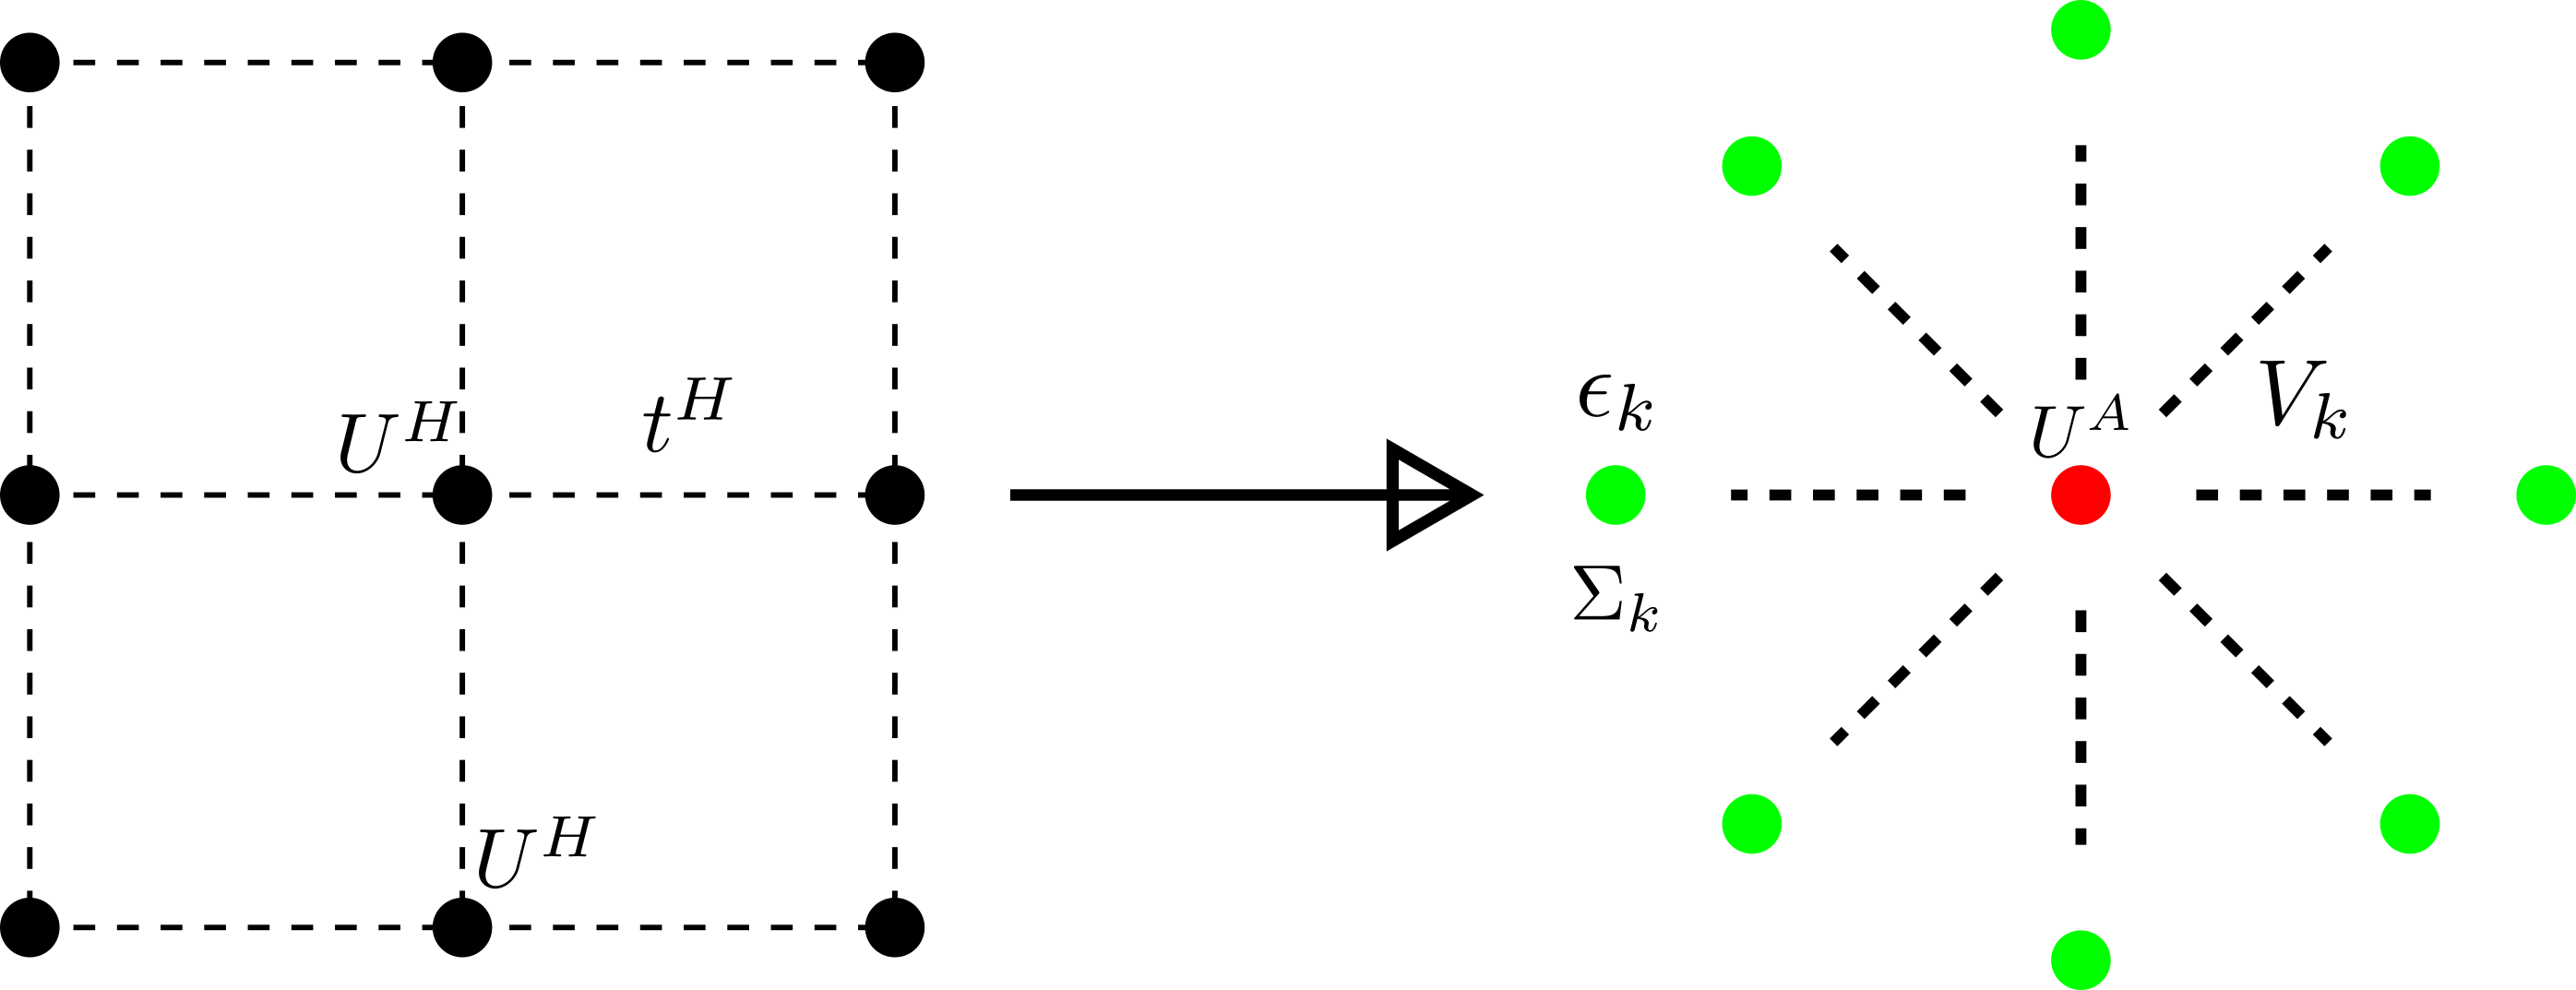
\includegraphics[width=0.8\textwidth]{../figures/cluster-bath.png}
	\caption{\textit{Left}: Full Hubbard model lattice with onsite repulsion $U^H$ on all sites and hopping between nearest neighbour sites with strength $t^H$. \textit{Right}: Extraction of the auxiliary (cluster+bath) system from the full lattice. The central site on left becomes the impurity site (red) on the right (with an onsite repulsion $\epsilon_d$), while the rest of the $N-1$ sites on the left form a conduction bath (green circles) (with dispersion $\epsilon_k$ and correlation modelled by the self-energy $\Sigma_k(\omega)$) that hybridizes with the impurity through the coupling $V$.}
	\label{cluster-bath}
\end{figure}
\textit{It should be noted that any reasonable choice of the cluster and bath would break the translational symmetry of the full model. To allow computing quantities, one would need to make the bath (which is a much larger system) simpler than the cluster (which is a single site). This distinction breaks the translational symmetry of the Hubbard model. For eg., if one chooses eq.~\ref{clus_bath_siam} as the auxiliary system, then the fact that the impurity has an onsite correlation while the bath only has a global capacitative cost $(\sim U_b N^2)$ means we have broken the symmetry between the cluster and the bath.}

The algorithm of DMFT then involves starting with some local self-energy of the bath, \(\Sigma(\omega)\), and using an impurity solver to calculate the impurity Greens function in the presence of this self-energy. This impurity Greens function is then used to calculate the impurity self-energy \(\Sigma_d(\omega)\), and the self-energy of the bath is then set equal to this impurity self-energy: \(\Sigma(\omega) = \Sigma_d(\omega)\), because we expect, on grounds of the lattice symmetry, that the impurity is the same as any other site in the bath. This is said to be the self-consistency step, because the bath self-energy is completely determined only at the end. With this updated bath self-energy, one then repeats the entire process until there is no further change in the bath self-energy at the self-consistency step.

 The present method intends to calculate the quantities in a different fashion. We first obtain an auxiliary model ($H_{Cl}$) by choosing a cluster of correlated sites that are hybridised with a bath through one-particle and two-particle exchange terms. The bath may additionally have local correlations. Then, we carry out a URG analysis of this auxiliary model to obtain a stable fixed point effective Hamiltonian:  $H^{*}_{CL} = \left[\mathcal{U}_{CL} H_{CL} \mathcal{U}_{CL}^\dagger \right]$.
% We start with a SIAM (with a correlated bath having a non-trivial self-energy), and solve it using the unitary renormalisation group approach to get to a fixed-point Hamiltonian. The fixed point Hamiltonian will in general involve the impurity site (with renormalised parameters $\epsilon_d^*, U^*$) interacting with a smaller number of momentum states.
% At this point, we will assume that we have a Hubbard model in mind that has motivated a correlated SIAM as the auxiliary system, and we have performed renormalisation group analysis on this auxiliary system to get down to an effective Hamiltonian. We will also assume that the parameters of the auxiliary system have been chosen such that in the effective Hamiltonian, the impurity and zero mode have the same onsite repulsion: $U^A = U^A_z$ (this is required for translational invariance).
% \\\\
% To obtain a comparatively simple but physically well-motivated auxiliary model, we identify $\sum_k c_k = \sqrt N c_0$; \(c_0\) is the operator for the zeroth site (the site nearest to the impurity). We will call the set of all \(N-2\) sites apart from the impurity and this zeroth site as the "effective bath". The fixed point Hamiltonian can be separated into these parts: an isolated impurity part, an isolated zeroth site part, an isolated effective bath part, hopping between impurity and the zeroth site and hopping between the zeroth site and the effective bath. \textit{As a simplification, we will ignore the correlation term \((U)\) on the effective bath}. In preparation of a symmetrization procedure, we will relabel the impurity site as 0, and the zeroth site as 1. With all these steps, the Hamiltonian takes the form:
% \begin{equation}\begin{aligned}
% 	\underbrace{U^A\tau_{0 \uparrow}\tau_{0 \downarrow} + U^A\tau_{1 \uparrow}\tau_{1 \downarrow}}_\text{imp. \& zero-mode isolated} - \underbrace{t^A\sum_{\sigma}\left(c^\dagger_{0\sigma}c_{1\sigma} + \text{h.c.}\right)}_\text{0-1 coupling} - \underbrace{t^A\sum_{j \in \atop{\text{NN of 1}}}\left(c^\dagger_{1\sigma}c_{j\sigma} + \text{h.c.}\right)}_\text{1 \& eff. bath coupling} - \underbrace{t^A \sum_{\left<ij \right>}^{\text{eff.} \atop{\text{bath}}}\left(c^\dagger_{i\sigma}c_{j\sigma} + \text{h.c.}\right)}_\text{eff. bath isolated}
% \end{aligned}\end{equation}
 \begin{figure}[htpb]
 	\centering
 	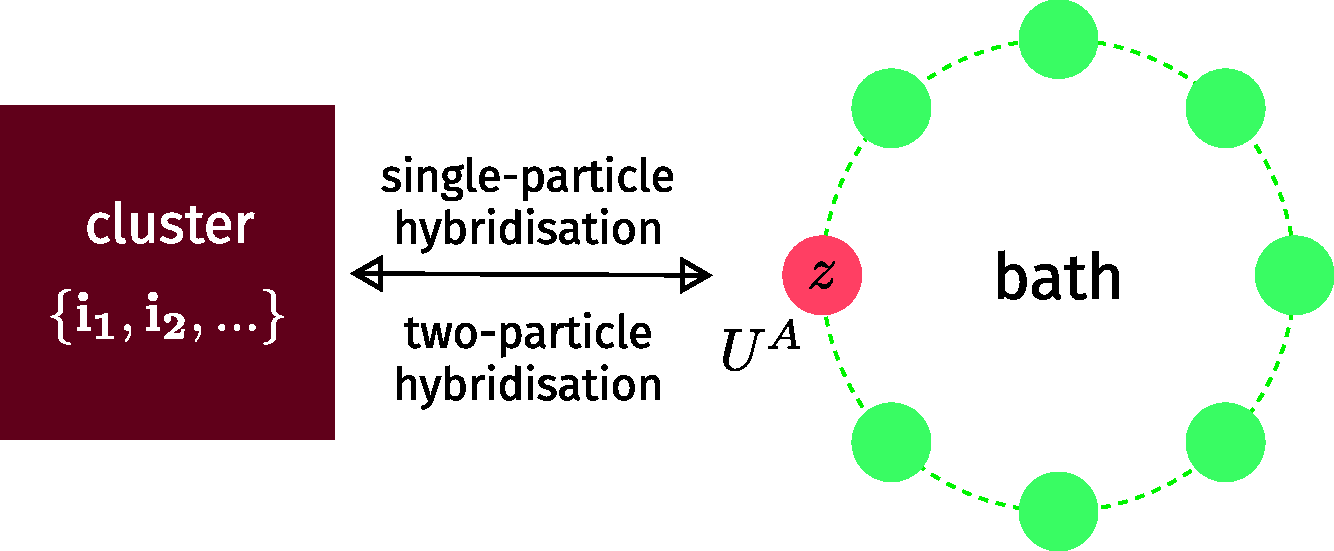
\includegraphics[width=0.6\textwidth]{../figures/gen_siam.pdf}
 	\caption{Cluster+bath construction of auxiliary model. It consists of a cluster (red square) hybridising with a bath (ring) by hopping into and out of the zeroth site (pink). The other sites (green) form the rest of the bath. Just the cluster and the zeroth site have onsite correlations.}
 \end{figure}
% This Hamiltonian is depicted in fig.~\ref{and_mol}. Such a Hamiltonian is, however, explicitly asymmetric between the sites 0 and 1 (the effective bath couples only to 1). To rectify that, we will symmetrize the coupling between the effective bath and the sites 0 and 1, by exchanging the sites 0 and 1. The resultant Hamiltonian is
% \begin{equation}\begin{aligned}
% 	\underbrace{U^A\tau_{0 \uparrow}\tau_{0 \downarrow} + U^A\tau_{1 \uparrow}\tau_{1 \downarrow} - t^A\sum_{\sigma}\left(c^\dagger_{0\sigma}c_{1\sigma} + \text{h.c.}\right)}_\text{2-site Hubbard model} +\underbrace{- t^A\sum_{j \in \atop{\text{NN of 1}}}\left(c^\dagger_{1\sigma}c_{j\sigma} + \text{h.c.}\right)- t^A\sum_{j \in \atop{\text{NN of 0}}}\left(c^\dagger_{0\sigma}c_{j\sigma} + \text{h.c.}\right)}_\text{dimer \& eff. bath coupling} \\
% 	- \underbrace{t^A \sum_{\left<ij \right>}^{\text{eff.} \atop{\text{bath}}}\left(c^\dagger_{i\sigma}c_{j\sigma} + \text{h.c.}\right)}_\text{eff. bath isolated}
% \end{aligned}\end{equation}
% % The motivation for extracting the zero mode is that it leads to a very simple effective Hamiltonian (the asymmetric Anderson molecule) without losing much of the low energy physics.
% To further simplify this Hamiltonian, \textit{we will combine the nearest neighbour sites of \(1\) and \(0\) into a single site}.
% \begin{equation}\begin{aligned}
% 	c_z \equiv \left(\sum_{j \in \atop{\text{NN of 1}}} + \sum_{j \in \atop{\text{NN of 0}}}\right)c_{j}
% \end{aligned}\end{equation}
% This single site will act as the zeroth site of the effective bath, and it means that both sites of the Hubbard dimer hybridizes with the effective through just a single site. With this assumption, the Hamiltonian for "a Hubbard dimer hopping into an effective bath" takes the simple form
% \begin{equation}\begin{aligned}
% 	\label{dimer_p_bat}
% 	\tilde H^D = H^D(0,1) - t^D \sum_{\sigma}\left(c^\dagger_{0\sigma}c_{z\sigma} + c^\dagger_{1\sigma}c_{z\sigma} + \text{h.c.}\right) + \sum_{\vec k}^\text{eff. bath}\epsilon_{\vec k}\hat n_{\vec k}
% \end{aligned}\end{equation}
% \(H^D(0,1)\) is the Hubbard dimer Hamiltonian (shown in fig.~\ref{hubb-dim}):
% \begin{equation}\begin{aligned}
% 	\label{dimer_ham}
% 	H^D(0,1) \equiv -t^D\sum_\sigma\left( c^\dagger_{0\sigma}c_{1\sigma} + \text{h.c.} \right) + U^D\left( \tau_{0 \uparrow}\tau_{0 \downarrow} + \tau_{1 \uparrow}\tau_{1 \downarrow}\right)
% \end{aligned}\end{equation}
% \begin{figure}[htpb!]
% 	\centering
% 	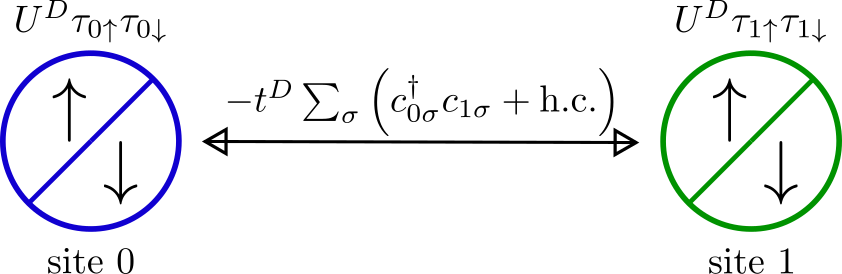
\includegraphics[width=0.4\textwidth]{../figures/hubb_dim.png}
% 	\caption{Hubbard dimer schematic version. It again consists of two sites, like the Anderson molecule, but now both sites have onsite repulsion, and their is again inter-site hopping.}
% 	\label{hubb-dim}
% \end{figure}
% This entire procedure is depicted in fig.~\ref{dimer-bath}.
% \begin{figure}[htpb]
% 	\centering
% 	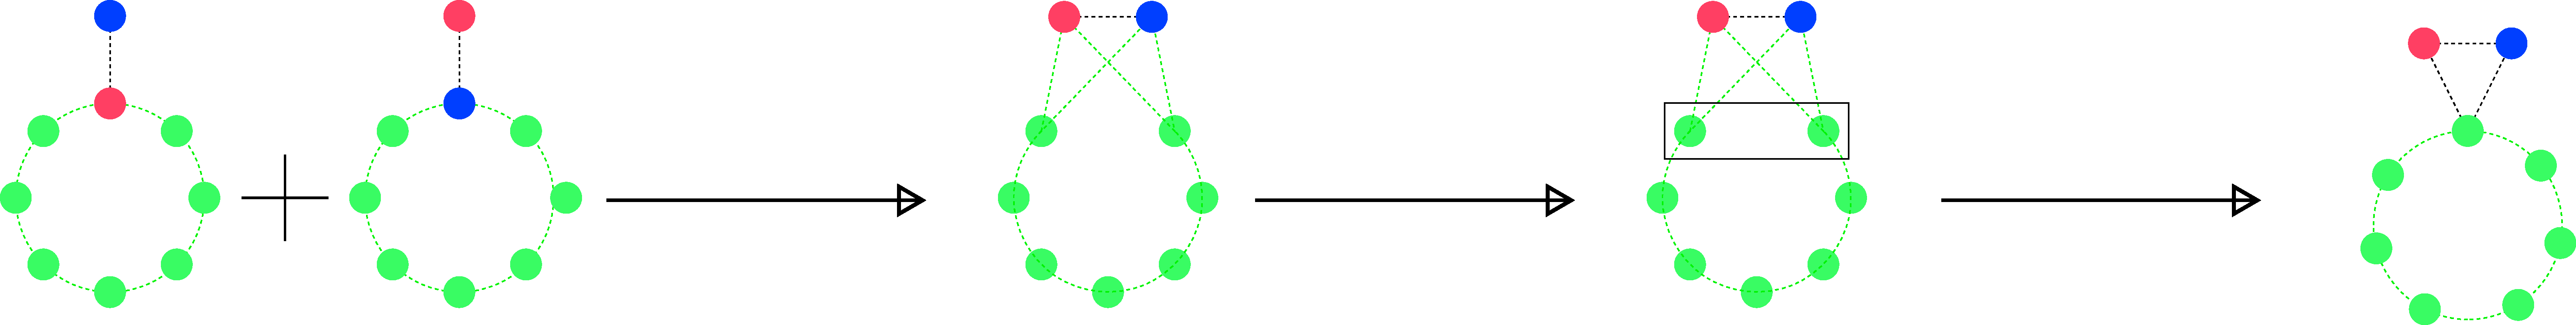
\includegraphics[width=\textwidth]{../figures/dimer_bath.pdf}
% 	\caption{The process of symmetrizing the Rg fixed point Hamiltonian and then creating a dimer+bath Hamiltonian. We first add the asymmetric Hamiltonians to get a symmetrized Hamiltonian. In the symmetrized Hamiltonian, the dimer has \(w\) entry points into the bath, \(w\) being the coordination number of the lattice. We then merge these \(w\) lattice sites (enclosed in the black box) into a single lattice site.}
% 	\label{dimer-bath} 
% \end{figure}
% We  can thus obtain a family of Hamiltonians \(\tilde H^D(i,j)\) obtained by setting \(0\) and \(1\) by setting the two sites of the dimer to any nearest-neighbour \(i,j\) on the lattice and the effective bath to the rest \(N-2\) sites of the lattice. 
The next step in the programme is to tile the real-space lattice with this cluster+bath Hamiltonian \(\tilde H\) to restore translational invariance (shown in a later section), and obtain a new bulk Hamiltonian for correlated electrons, $\tilde H = T\left[ \tilde H^{*}_{CL} \right] T^{-1}$, where $T$ denotes the operator that performs the set of iterative real-space translations, and enables the cluster-bath (auxiliary model) Hamiltonian to span the target real-space lattice. Given a general auxiliary model Hamiltonian \(H_\text{CL}^*\), the result of tiling can be written very generally as
 \begin{equation}\begin{aligned}
	 \tilde H = \sum_{\left\{i_1,i_2,...\right\}} H^*_\text{CL}\left(\left\{i_1,i_2,...\right\}\right)
 \end{aligned}\end{equation}
where \(\left\{i_1,i_2,...\right\}\) represents the indices for the members of the cluster. To reiterate, what that means is that we have placed the cluster+bath system at all lattice point sets \(\left\{i_1,i_2,...\right\}\) to reconstruct a new model of correlated electsons. If we assume that the tiling mostly rectifies the explicit symmetry-breaking made while choosing the auxiliary system as well as dropping the correlation on the bath sites, we can write
 \begin{equation}\begin{aligned}
 	\label{app2}
 	\tilde H = \mathcal{U} H_{CL} \mathcal{U}^{-1} = T\left[\mathcal{U}_{CL} H_{CL} \mathcal{U}_{CL}^\dagger \right]T^{-1}~,
 \end{aligned}\end{equation}
 where $\mathcal{U} = T \mathcal{U}_{CL}$ is some transformation that is either a unitary, or, at the very least, a similarity transformation that maps from the original auxiliary model Hamiltonian to the reconstructed bulk Hamiltonian. The answer to how closely $\tilde H$ approximates a target model of correlated electrons lies in (i) the choice of the cluster-bath construction of the auxiliary model, and (ii) the accuracy of the URG procedure on the auxiliary model. 
 %The existence of $U$ is contingent on how good the approximations are.\\\\
% We mention the two approximations made along the entire journey from the original Hubbard model to the reconstructed one here.
% \begin{itemize}
% 	\item We have replaced the full Hubbard model by an auxiliary system described by the SIAM Hamiltonian in eq.~\ref{clus_bath_siam}. The accuracy of this assumption is determined by the choice of the SIAM parameters, particular the self-energy and repulsion of the bath. As discussed before, the very choice of th cluster and bath spoil the translational invariance of the parent model.
% 	\item We then perform a unitary RG on $H^A$. This leads to a fixed-point Hamiltonian $\mathcal{U}_A H^A \mathcal{U}_A^\dagger$. At this point, we go from the fixed point Hamiltonian to the dimer+bath Hamiltonian in eq.~\ref{dimer_p_bat}. If we represent this transformation from the fixed point Hamiltonian to the Hamiltonian in eq.~\ref{dimer_p_bat} by an operator \(Z\), we can write $H^D = Z\left[\mathcal{U}_A H^A \mathcal{U}_A^\dagger \right] Z^{-1}$. This constitutes the second approximation we make.
% \end{itemize}


\section{What is the minimal impurity model for a Mott MIT?}
A correlated single impurity site connected with a non-interacting bath with a uniform density of states leads to a well-defined Kondo resonance at low temperatures, as seen in the impurity spectral function. Increasing the impurity correlation \(U\) only serves to reduce the width of the central peak at the cost of the appearance of side bands at energy scales of the order of \(U\), but the resonance never dies. The situation is however different if the impurity is embedded in a correlated conduction bath with a non-trivial density of states. For the case of a conduction band with the DOS shown in the right of the figure below, the impurity hybridises into a reduced bandwidth because of the correlation on the lattice. This difference is what leads to a metal-insulator transition of a bulk Hubbard model under dynamical mean-field theory (DMFT). Under self-consistency, the non-interacting bath gets modified into one with a highly-correlated self-energy. At low \(U\), the impurity spectral function remains gapless, but at sufficiently large \(U\), the bath is able to kill the Kondo resonance and lead to an insulating state. \textit{This leaves open the following question: What is the minimal correlation one can insert into the non-interacting bath (of a single-impurity Anderson model) that can capture both the metallic and insulating phases of the bulk model?}
\cite{held_2013}

\begin{figure}[htpb]
\centering
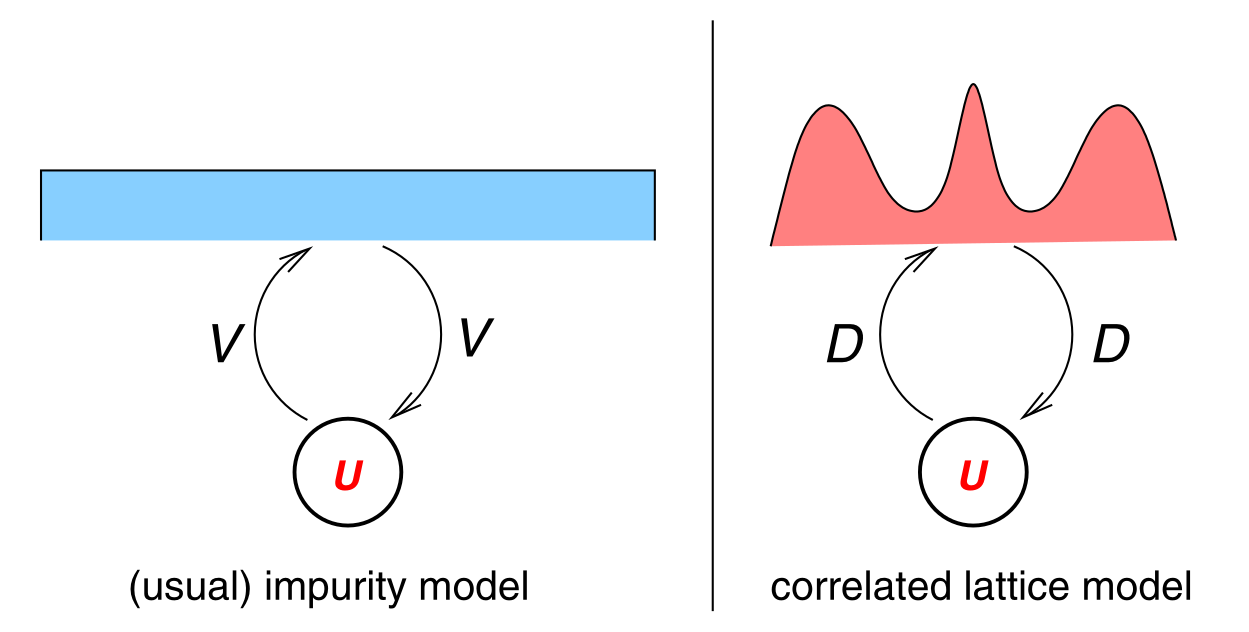
\includegraphics[width=0.5\textwidth]{../figures/correlated_bath.png}
\caption{"Comparison of the usual Anderson
impurity model of a strongly interacting site coupled via $V$ to
an uncorrelated featureless and wide conduction-electron band
(left-hand side) and the Hubbard model situation (right-hand
side). In the latter case, an electron leaving a correlated site
moves within the strongly correlated and narrow band of the
central peak. In this situation there is a kink at the effective
Kondo energy scale which is smaller than the width of the
narrow band." Image and caption source in footnote.}
\end{figure}

This is an attempt to obtain various quantities like Greens functions, self-energies, spectral functions and (if possible) energies and wavefunctions of the Hubbard model, using a cluster-bath approach. The cluster-bath system is taken to be a single-impurity Anderson model with a correlated bath. The correlation will be brought about in two ways: a self-energy $\Sigma(k,\omega)$ of the bath, and a double occupancy repulsion cost $U_b$. The Hubbard and the correlated single-impurity Anderson models are defined using the Hamiltonians
\begin{align}
H_\text{hubb} &= -t^H\sum_{\sigma,\left<i,j \right>}\left(c^\dagger_{i\sigma} c_{j\sigma} + \text{h.c.}\right) + U^H\sum_i \hat n_{i \uparrow} \hat n_{i \downarrow} - \mu^H \sum_{i\sigma}\hat n_{i\sigma}\\
H_\text{siam} &= \sum_{k\sigma}\left[\epsilon_k + \Sigma(k,\omega)\right]\hat n_{k\sigma} + \epsilon_d^A \sum_\sigma\hat n_{d\sigma} + U^A \hat n_{d \uparrow} \hat n_{d \downarrow} + U_b \sum_{kk^\prime}\hat n_k \hat n_{k^\prime} -t^A\sum_{k\sigma}\left(c^\dagger_{d\sigma}c_{k\sigma} + \text{h.c.}\right) \label{clus_bath_siam}
\end{align}
Broadly speaking, the method involves first solving the SIAM using a unitary renormalisation group approach, to get the low energy effective theory, and then combining the low energy Hamiltonians in a symmetrized fashion to get the Hamiltonian for the Hubbard model lattice. It is reminescent of dynamical mean-field theory (DMFT) - both involve an impurity-solver that solves an auxiliary system. The difference, however, lies in the following points:
\begin{itemize}
	\item While DMFT primarily works with Greens functions and self-energies, this method involves Hamiltonians. The impurity-solver in DMFT provides an impurity Greens function (which is then equated with the local Greens function of the bath), while the impurity-solver in this method actually provides a low energy Hamiltonian.
	\item The final step of DMFT is the self-consistency equation, where the impurity and bath-local quantities are set equal. This ensures all sites, along with the impurity site, have the same self-energy, something which is required on grounds of  translational invariance. The present method, however, brings about the translational invariance in a different way. It symmetrizes the Hamiltonians itself, such that all quantites then derived from the Hamiltonian are then guaranteed to have the symmetry.
\end{itemize}
The meaning of each of these statements will become clearer when we describe the method in more detail.


\chapter{Physics of the generalised single-impurity Anderson model}
\section{Introduction of spin-exchange and charge isospin-exchange interactions into the SIAM: the generalised SIAM}
We will now study the generalised SIAM obtained by introducing spin-exchange and charge isospin-exchange interactions between the impurity and the conduction bath. Such terms are generated when one does a Schrieffer-Wolff transformation on the SIAM, but we will find it prudent to keep these terms in the bare model itself.

The spin-exchange interaction has the form
\begin{equation}\begin{aligned}
	J \vec{S_d}\cdot\vec{s} = J \left[S_d^z s^z + \frac{1}{2}\left( S_d^+ s^- + S_d^- s^+ \right) \right] ~,
\end{aligned}\end{equation}
where \(\vec S_d = \left(S_d^x, S_d^y, S_d^z\right) = \sum_{\alpha\beta}\vec \sigma_{\alpha\beta}c^\dagger_{d\alpha}c_{d\beta}\) is the impurity spin operator, \(\vec s = \sum_{kk^\prime\alpha\beta}\vec \sigma_{\alpha\beta}c^\dagger_{k\alpha}c_{k^\prime\beta}\) is the spin operator for the conduction bath and \(J\) is the spin-exchange coupling. The bath spin operator actually acts locally, as can be seen by Fourier transforming to real space (using the definition \(f(k) = \frac{1}{\sqrt N}\sum_r g(r)\exp(ikr)\)):
\begin{equation}\begin{aligned}
	\vec s = \sum_{k k^\prime r r^\prime} \frac{1}{N} e^{ikr - ik^\prime r^\prime} \vec \sigma_{\alpha\beta} c^\dagger_{r\alpha} c_{r^\prime\beta} = \sum_{rr^\prime}\frac{1}{N}\vec \sigma_{\alpha\beta} c^\dagger_{r\alpha} c_{r^\prime\beta} N \delta(r)\delta(r^\prime) = \vec \sigma_{\alpha\beta} c^\dagger_{0\alpha} c_{0\beta}
\end{aligned}\end{equation}

In order to introduce the charge isospin coupling, we define the Nambu spinor \cite{anderson1958random,nambu_1960} \(\psi^k = \left( c_{k\uparrow} \quad c^\dagger_{k\downarrow} \right)\), and the charge isospin \cite{zitko_2006} for the mobile conduction electrons
\begin{equation}\begin{aligned}
\vec C = \sum_{kk^\prime} {\psi^k}^\dagger \vec S \psi^{k^\prime} = \frac{1}{2}\sum_{kk^\prime\alpha\beta} {\psi^k_\alpha}^\dagger \vec \sigma_{\alpha\beta} \psi^{k^\prime}_\beta
\end{aligned}\end{equation}
The various components of the isospin are
\begin{equation}\begin{aligned}
	C^z &= \sum_{kk^\prime\sigma}\frac{1}{2} {\psi^k_\sigma}^\dagger \sigma^z_{\sigma\sigma} \psi^{k^\prime}_\sigma = \frac{1}{2}\sum_{kk^\prime\sigma}\left(c^\dagger_{k\sigma}c_{k^\prime \sigma} - \frac{1}{2}\delta_{kk^\prime}\right)\label{diagonalCz}\\
	C^x &= \sum_{kk^\prime\sigma}\frac{1}{2} {\psi^k_\sigma}^\dagger \sigma^x_{\sigma\overline\sigma} \psi^{k^\prime}_{\overline\sigma} = \sum_{kk^\prime\sigma} \frac{\sigma}{4}\left( c^\dagger_{k\sigma}c^\dagger_{k^\prime\overline\sigma} + \text{h.c.} \right) \\
	C^y &= \sum_{kk^\prime\sigma}\frac{1}{2} {\psi^k_\sigma}^\dagger \sigma^y_{\sigma\overline\sigma} \psi^{k^\prime}_{\overline\sigma} = \sum_{kk^\prime\sigma} - \frac{i\sigma}{4}\left( c^\dagger_{k\sigma}c^\dagger_{k^\prime\overline\sigma} - \text{h.c.} \right)\\
\end{aligned}\end{equation}
It is easy to verify that these operators satisfy the SU(2) commutation algebra. For example, if we write \(C^x = A + A^\dagger\) and \(C^y = B + B^\dagger\), then \(\left[ C^x, C^y \right] = \left[ A, B^\dagger \right] - \text{h.c.}\), where
\begin{equation}\begin{aligned}
	\left[ A, B^\dagger \right] = \frac{1}{4}\sum_{kk^\prime,qq^\prime}\left[ c^\dagger_{k\uparrow}c^\dagger_{k^\prime \downarrow}, i c_{q^\prime \downarrow}c_{q \uparrow} \right] = \frac{i}{4}\sum_{kq}\left(c^\dagger_{k\uparrow}c_{q \uparrow} - c_{k \downarrow}c^\dagger_{q \downarrow}\right)
\end{aligned}\end{equation}
and therefore
\begin{equation}\begin{aligned}
	\implies \left[ C^x, C^y \right] = \frac{i}{2}\sum_{kq}\left(c^\dagger_{k\uparrow}c_{q \uparrow} - c_{k \downarrow}c^\dagger_{q \downarrow}\right) = i C^z
\end{aligned}\end{equation}
There are similar operators for the impurity electron:
\begin{equation}\begin{aligned}
	\psi_d = \left( c_{d\uparrow} \quad c^\dagger_{d\downarrow}\right), &&\vec C_d = \frac{1}{2}\sum_{\beta} {\psi_{d,\alpha}}^\dagger \vec \sigma_{\alpha\beta} \psi_{d,\beta}
\end{aligned}\end{equation}
The full charge-Kondo interaction can now be written down in terms of these isospins:
\begin{equation}\begin{aligned}
	K \vec{C_d}\cdot\vec{C} = K \left[C_d^z C^z + \frac{1}{2}\left(C_d^+ C^-+ C_d^- C^+\right)\right]
\end{aligned}\end{equation}
where \(C^\pm \equiv C^x \pm iC^y\).
\begin{equation}\begin{aligned}
	C^+ = \sum_{kk^\prime} c^\dagger_{k\uparrow}c^\dagger_{k^\prime\downarrow}, && C^- = \sum_{kk^\prime}c_{k^\prime\downarrow}c_{k\uparrow}
\end{aligned}\end{equation}
The full generalised Anderson model Hamiltonian, at particle-hole symmetry, is
\begin{equation}\begin{aligned}
	\mathcal{H} = \sum_{k\sigma}\epsilon_k \tau_{k\sigma} + \epsilon_d \left( \hat n_{d \uparrow} - \hat n_{d \downarrow} \right) ^2 + \sum_{k\sigma} \left(V_{k} c^\dagger_{k\sigma} c_{d\sigma} + h.c.\right) +J \vec{S_d}\cdot\vec{s} + K \vec{C_d}\cdot\vec{C}
\end{aligned}\end{equation}

For the URG analysis, at each RG step, we decouple the electronic states \(q\beta\) on the \(k-\)space shell of radius\(\Lambda_j\). For simplicity, we will only consider those diagonal terms in the denominator that either have both \(q\beta\) and \(q\overline\beta\) or  both \(q\beta\) and \(d\) or both \(q\overline\beta\) and \(d\). Terms that have purely \(q\overline\beta\) will not be considered. Also, the scattering between just \(d\) and \(q\overline\beta\) can be ignored since it is diagonal in \(q\beta\). 
The diagonal (number-preserving) part is
\begin{equation}\begin{aligned}
	H_D = \sum_\beta\epsilon_q\tau_{q\beta} + \epsilon_d \left( \hat n_{d \uparrow} - \hat n_{d \downarrow} \right) ^2 + J S^z_ds^z_{q} + K C^z_d C^z_q\\
\end{aligned}\end{equation}
where \(s_q^z = \frac{1}{2}\left(\hat n_{q\uparrow} - \hat n_{q\downarrow}\right)\) and \(C_q^z = \frac{1}{2}\left(\hat n_{q \uparrow} + \hat n_{q \downarrow} - 1\right)\). The off-diagonal part is:
\begin{equation}\begin{aligned}
	H_X = \sum_{\beta=\uparrow,\downarrow}\left[V c^\dagger_{d\beta}c_{q\beta} + \frac{1}{2}J \sum_{k<\Lambda_N}\left\{\left(\hat n_{d \beta} - \hat n_{d \overline\beta}\right) \frac{1}{2} c^\dagger_{k\beta}c_{q\beta} + c^\dagger_{d\beta}c_{d\overline\beta}c^\dagger_{k\overline\beta}c_{q \beta}\right\} + \frac{1}{2}K \sum_{k<\Lambda_N}\left\{\left(\hat n_d -1\right)\frac{1}{2}c^\dagger_{k\beta}c_{q\beta} + \right.\right.\\
\left.\left.c^\dagger_{d\beta}c^\dagger_{d\overline\beta}c_{k\overline\beta}c_{q\beta}\right\}\right] + \text{h.c.}~.
\end{aligned}\end{equation}

\begin{figure}[htpb]
	\centering
	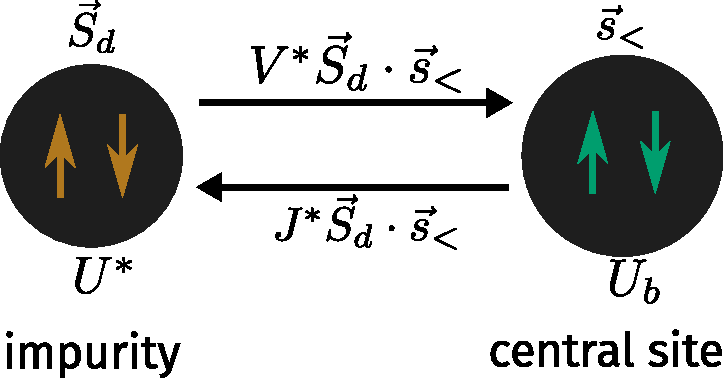
\includegraphics[width=0.5\textwidth]{../figures/zeromode.pdf}
	\caption{While we have studied the full model under renormalisation group, often we will turn to a simplified zero-bandwidth version of the model that is obtained by ignoring the kinetic energy part of the Hamiltonian. This zero-bandwidth model is effectively a two site model.}
\end{figure}

\section{RG equations for generalised SIAM}
\begin{equation}\begin{aligned}
	\Delta \epsilon_d &= 2V^2 n_j\left(\frac{1}{\omega - \frac{D}{2} + \epsilon_d + \frac{K}{4}} - \frac{1}{\omega - \frac{D}{2} - \epsilon_d + \frac{J}{4}}\right) + \frac{n_j}{2}\left(\frac{J^2}{\omega - \frac{D}{2} + \frac{J}{4}} - \frac{K^2}{\omega - \frac{D}{2} + \frac{K}{4}}\right),\\
	\Delta V &= -\frac{3n_j V}{8}\left[J\left(\frac{1}{\omega - \frac{D}{2} + \frac{J}{4}} + \frac{1}{\omega - \frac{D}{2} - \epsilon_d + \frac{J}{4}}\right) + K \left(\frac{1}{\omega - \frac{D}{2} + \frac{K}{4}} + \frac{1}{\omega - \frac{D}{2} + \epsilon_d + \frac{K}{4}}\right)\right],\\
	\Delta J &= -\frac{n_j J^2}{\omega - \frac{D}{2} + \frac{J}{4}},\\ 
	\Delta K &= -\frac{n_j K^2}{\omega - \frac{D}{2} + \frac{K}{4}}
\end{aligned}\end{equation}
In terms of \(U = -2\epsilon_d\), the equations become
\begin{gather}
	\Delta U = 4V^2 n_j\left(\frac{1}{d_1} - \frac{1}{d_0}\right) - n_j\left(\frac{J^2}{d_2} - \frac{K^2}{d_3}\right),\\
	\Delta V = -\frac{3n_j V}{8}\left[J\left(\frac{1}{d_2} + \frac{1}{d_1}\right) + K \left(\frac{1}{d_3} + \frac{1}{d_0}\right)\right],\\
	\Delta J = -\frac{n_j J^2}{d_2}, \quad\quad\Delta K = -\frac{n_j K^2}{d_3}
\end{gather}
\(d_i\) are the denominators:
\begin{equation}\begin{aligned}
	\label{denominators}
	d_0 = \omega - \frac{D}{2} - \frac{U}{2} + \frac{K}{4}, \quad d_1 = \omega - \frac{D}{2} + \frac{U}{2} + \frac{J}{4}, \quad d_2 = \omega - \frac{D}{2} + \frac{J}{4}, \quad d_3 = \omega - \frac{D}{2} + \frac{K}{4}
\end{aligned}\end{equation}

\section{Nature of coupling RG flows}
\subsection{Repulsive interaction on impurity: \(U>0\)}
For the Hamiltonians with positive on-site correlation, we will assume that the spin-exchange coupling is positive and charge isospin-exchange coupling is negative: \(J>0, K<0\). This choice is motivated by the signs of the corresponding terms when they are generated via a Schrieffer-Wolff transformation~\cite{schrieffer1966}. The impurity-bath hybridisation \(V\) is always positive. The sign of the couplings lead to inequalities among the denominators which we will utilise at various points. First of all, since \(U>0\), we have \(d_1 - d_2 = \frac{U}{2} > 0\). Secondly, since \(K<0\), we have \(d_2 - d_3 = \frac{J-K}{4} > 0\). And finally, we have \(d_3 - d_0 = \frac{U}{2} > 0\). Combining these, we can write
\begin{equation}\begin{aligned}
	\label{ineq_den}
	d_1 > d_2 > d_3 > d_0
\end{aligned}\end{equation}

The strong-coupling regime is defined as the range of values of \(\omega\) where the hybridisation is relevant. This is ensured by the assumption \(d_1<0\). From eq.~\ref{ineq_den}, we can then conclude that all denominators are negative: \(d_i = - |d_i|\). The simplest consequence of this is the RG flow of \(K\):
\begin{equation}\begin{aligned}
	\Delta K= -\frac{n_j K^2}{d_3} = \frac{n_j K^2}{|d_3|} > 0 \implies K_{j+1} > K_j \implies K_0 = -|K_0|, K^* \to 0
\end{aligned}\end{equation}
\(K_j\) is the value of \(K\) after the \(j^\text{th}\) RG step, \(K_0\) representing the bare value.
In other words, since \(d_3 < 0\), the RG equation for \(K\) provides an algebraic increment, and the negative \(K\) increases and flows towards zero. The \(*\) indicates a fixed point value. The isospin coupling is irrelevant in this regime, and we will ignore it.

The coupling \(J\), on the other hand, is relevant and flows from a small positive value towards a large value at strong-coupling.
\begin{equation}\begin{aligned}
	\Delta J= -\frac{n_j J^2}{d_2} = \frac{n_j J^2}{|d_2|} > 0 \implies J_{j+1} > J_j \implies J_0 \to \text{ large } J^* ~(\text{strong-coupling})
\end{aligned}\end{equation}
The value of \(J^*\) is obtained when the denominator \(d_2\) vanishes.

Because of the RG irrelevance of \(K\), we can simplify the RG equation for \(V\):
\begin{equation}\begin{aligned}
	\Delta V = -\frac{3n_j VJ}{8}\left(\frac{1}{d_2} + \frac{1}{d_1}\right) = \frac{3n_j VJ}{8}\left(\frac{1}{|d_2|} + \frac{1}{|d_1|}\right) > 0
\end{aligned}\end{equation}
Since both the denominators are positive, \(V\) is relevant. The fixed point value \(V^*\) is attained when the denominator \(d_1\) vanishes (\(d_1\) will vanish earlier than \(d_2\)).

We can compare the rate of flows of \(V\) and \(J\):
\begin{equation}\begin{aligned}
	\frac{\Delta V}{\Delta J} = \frac{3V}{8J}\left(1 + \frac{|d_2|}{|d_1|}\right) > \frac{3V}{4J}
\end{aligned}\end{equation}
There we used the fact that \(|d_2| > |d_1|\).
We finally come to the RG equation for \(U\):
\begin{equation}\begin{aligned}
	\Delta U = 4V^2 n_j\left(\frac{1}{d_1} - \frac{1}{d_0}\right) - n_j\frac{J^2}{d_2} = -4V^2\left(U + \frac{J}{4}\right)\frac{n_j}{d_0 d_1} - \frac{n_j J^2}{d_2}
\end{aligned}\end{equation}
For \(V>J\), we can expect \(U\) to be irrelevant. On the other hand, \(V<J\) makes \(U\) relevant.

In short, the \(U>0\) regime is characterised by an irrelevant isospin-exchange coupling \(K\) and a relevant spin-exchange coupling \(J\), and the following set of RG equations for the remaining couplings \(U\) and \(V\):
\begin{equation}\begin{aligned}
	\Delta U = 4V^2 n_j\left(\frac{1}{d_1} - \frac{1}{d_0}\right) - n_j\frac{J^2}{d_2}, \quad \Delta V = -\frac{3n_j VJ}{8}\left(\frac{1}{d_2} + \frac{1}{d_1}\right)
\end{aligned}\end{equation}

%\begin{figure}[htpb]
%	\centering
%	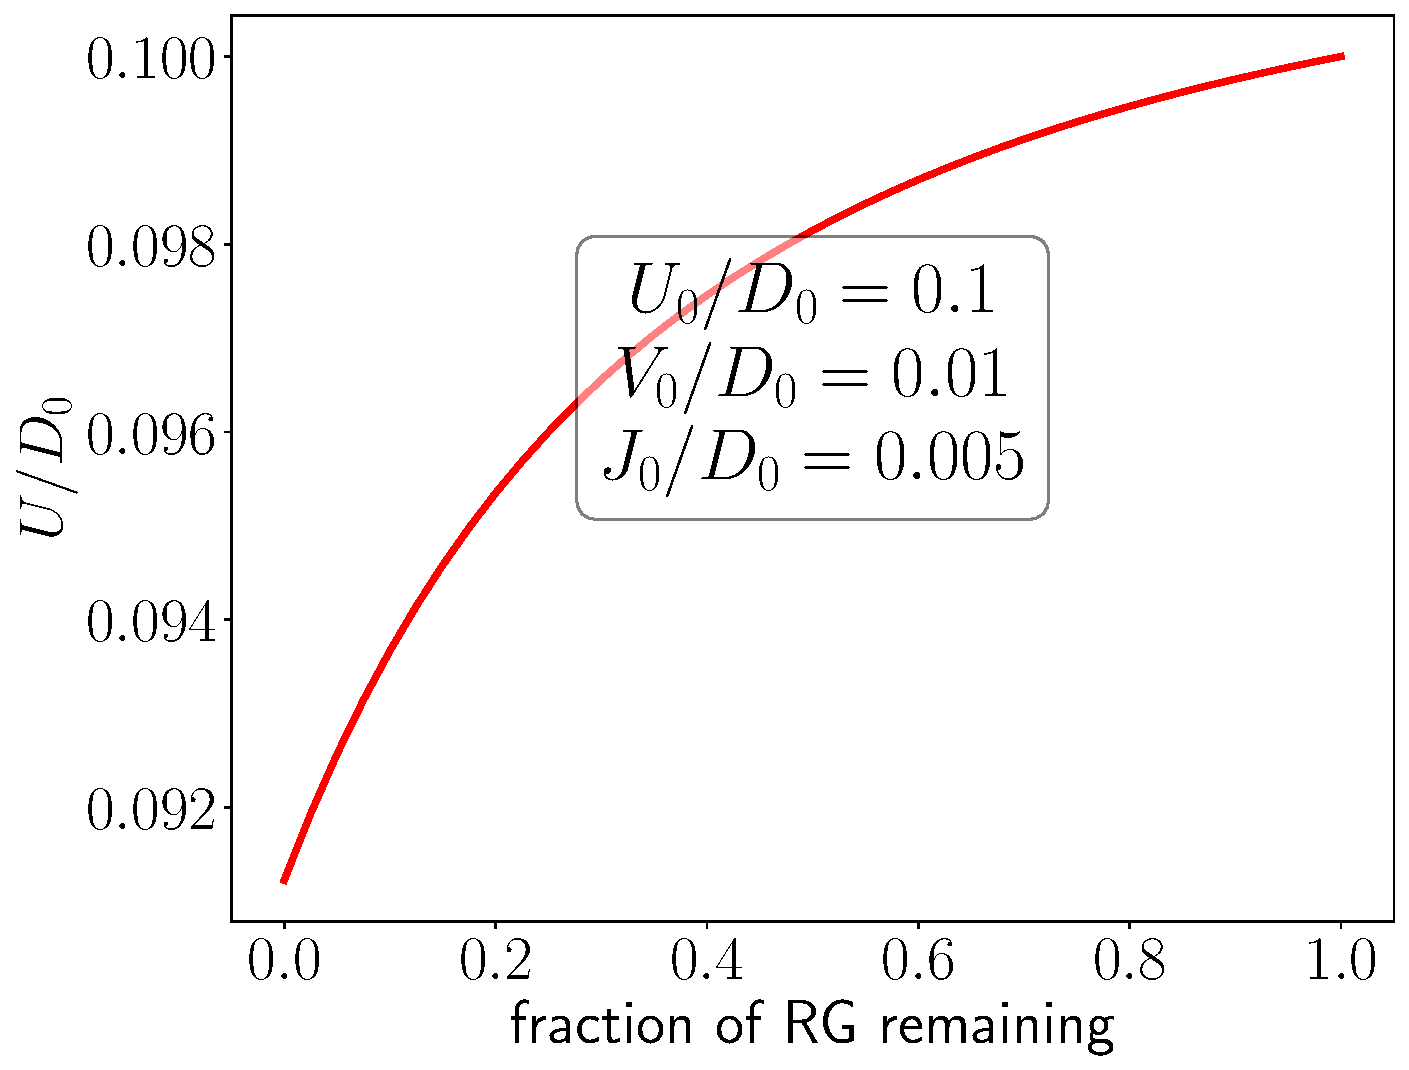
\includegraphics[width=0.32\textwidth]{../figures/U_irr,U>0,U.pdf}
%	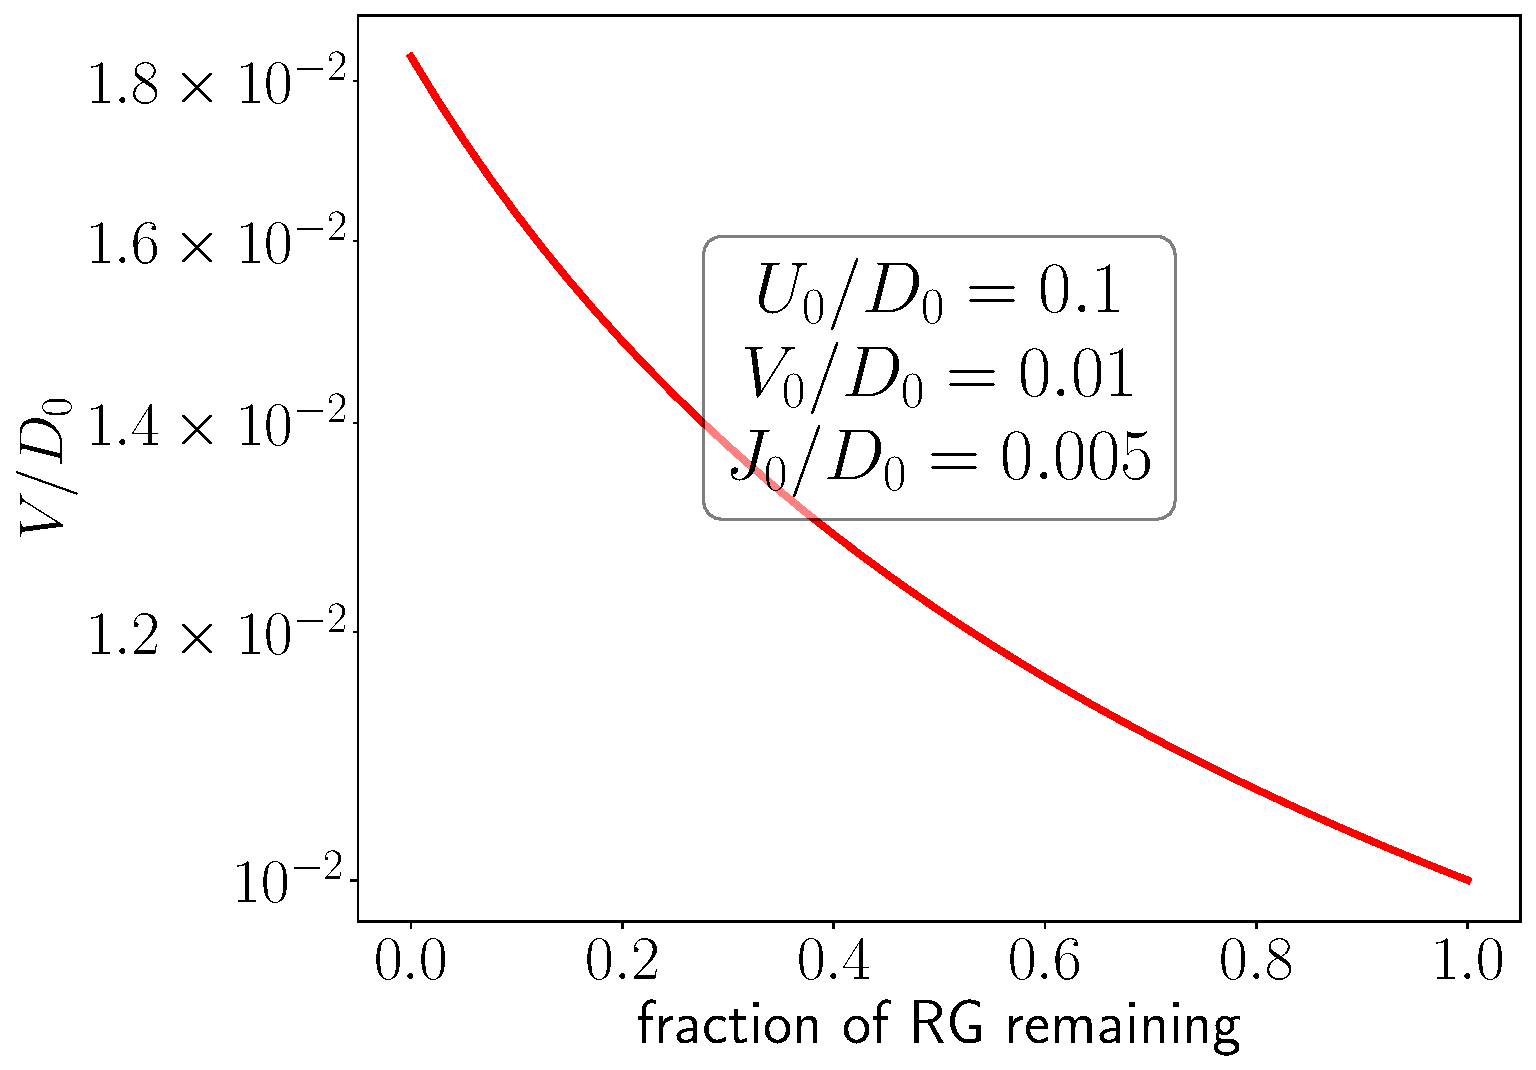
\includegraphics[width=0.32\textwidth]{../figures/U_irr,U>0,V.pdf}
%	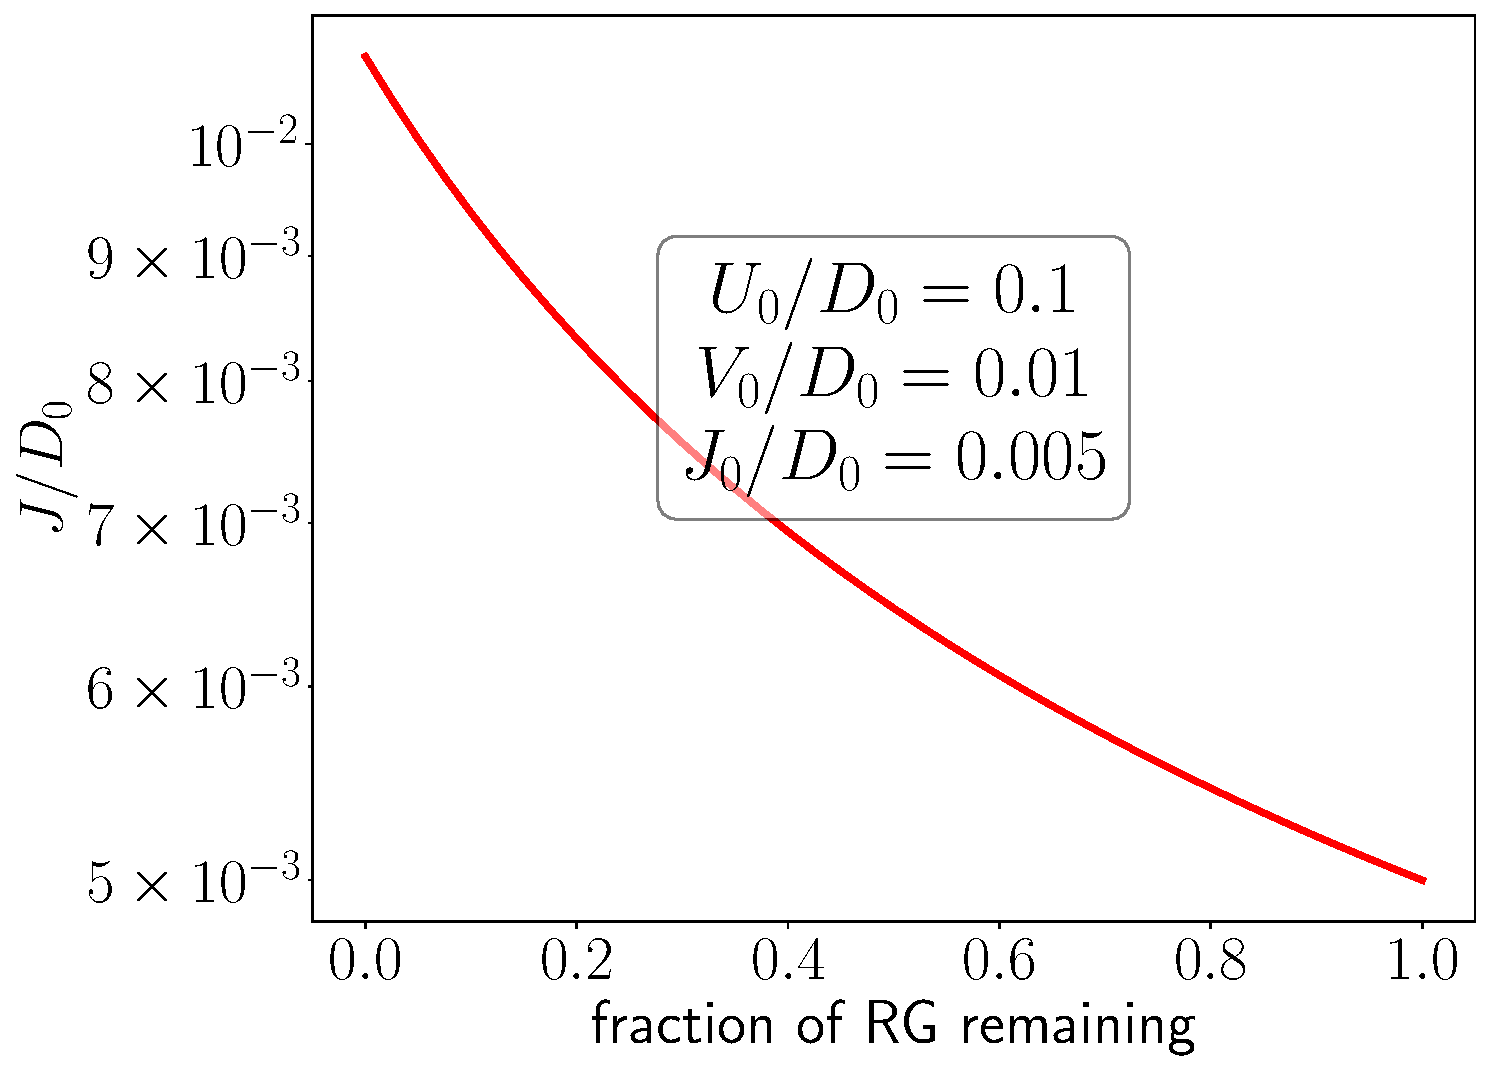
\includegraphics[width=0.32\textwidth]{../figures/U_irr,U>0,J.pdf}
%
%	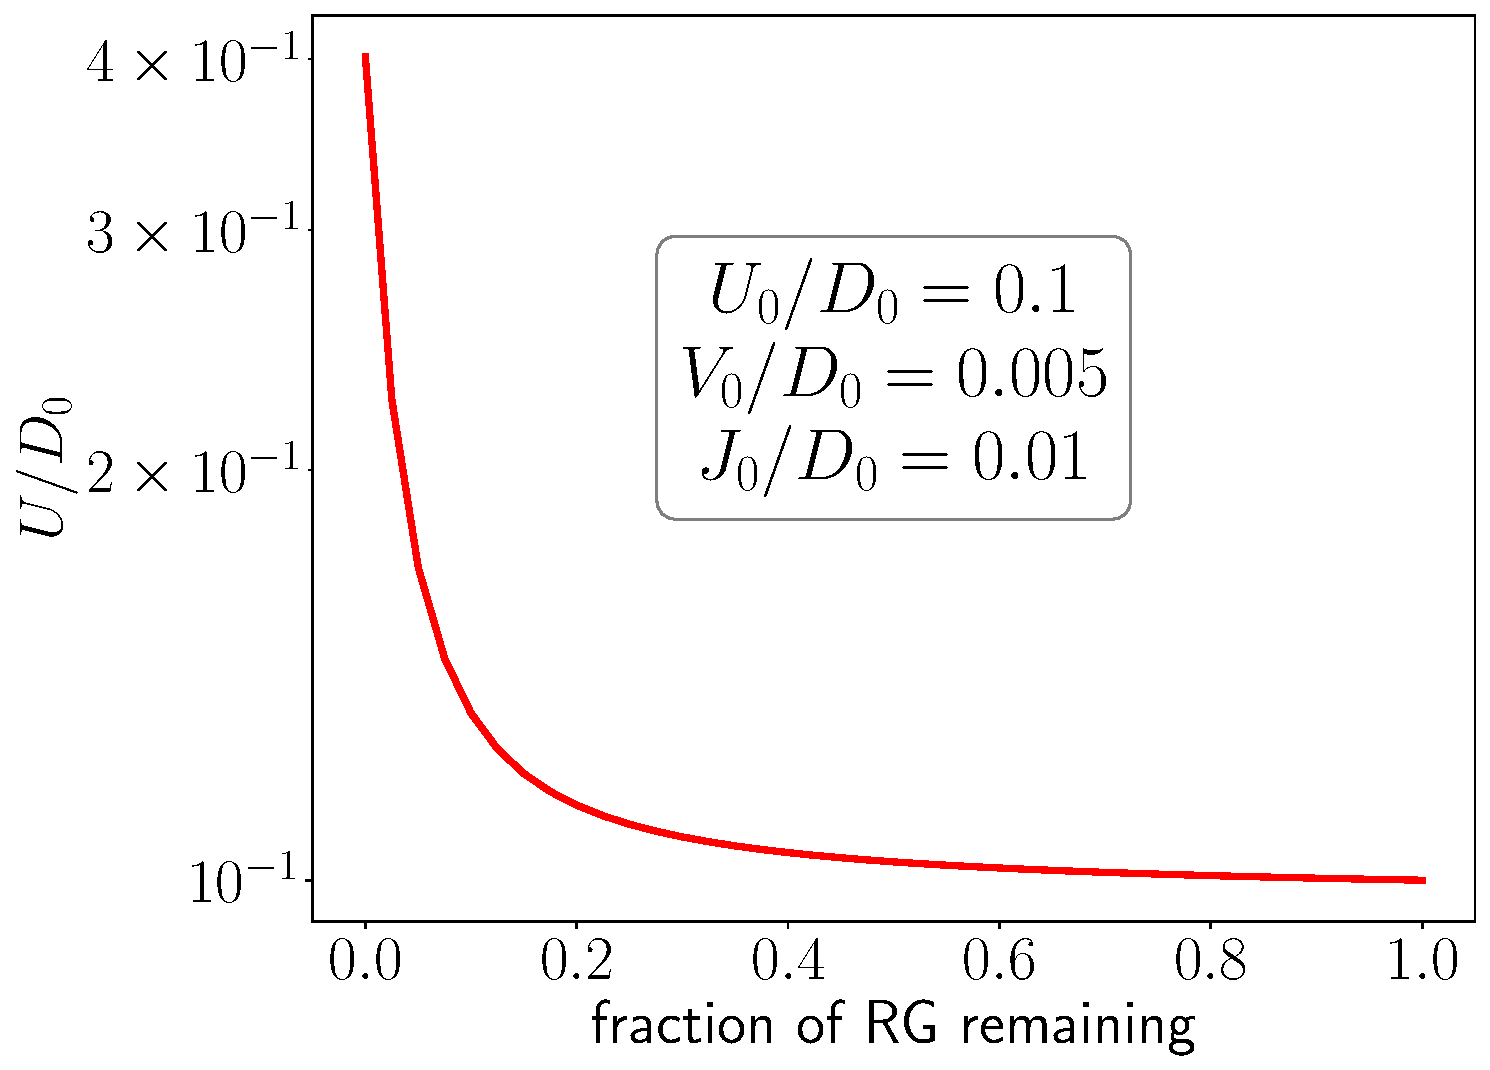
\includegraphics[width=0.32\textwidth]{../figures/U_rel,U>0,U.pdf}
%	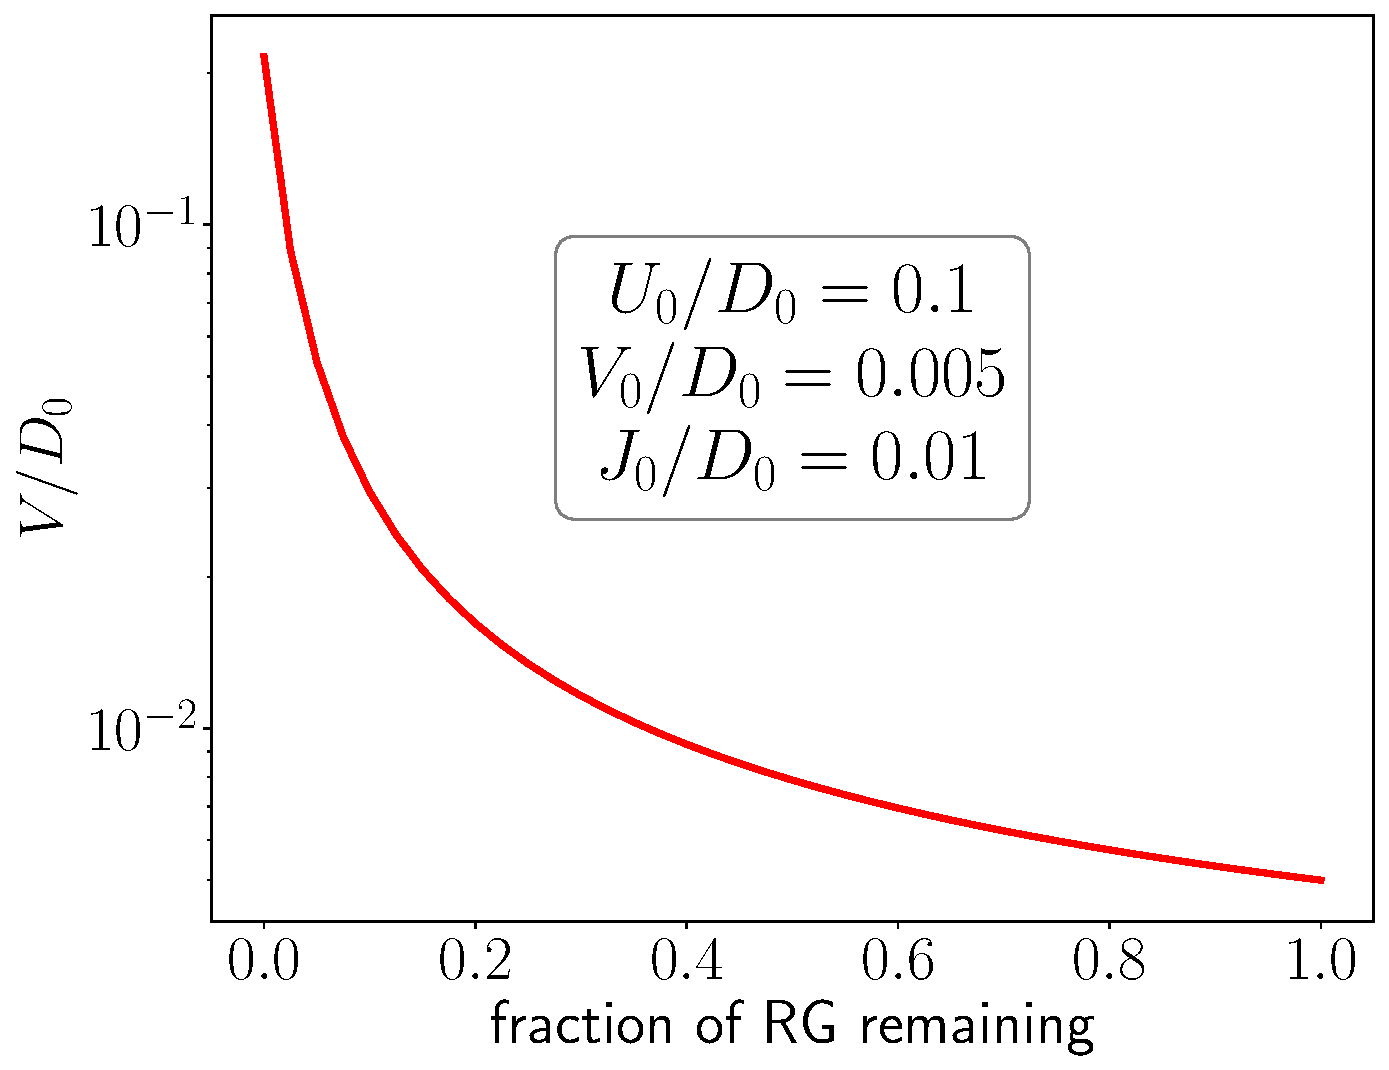
\includegraphics[width=0.32\textwidth]{../figures/U_rel,U>0,V.pdf}
%	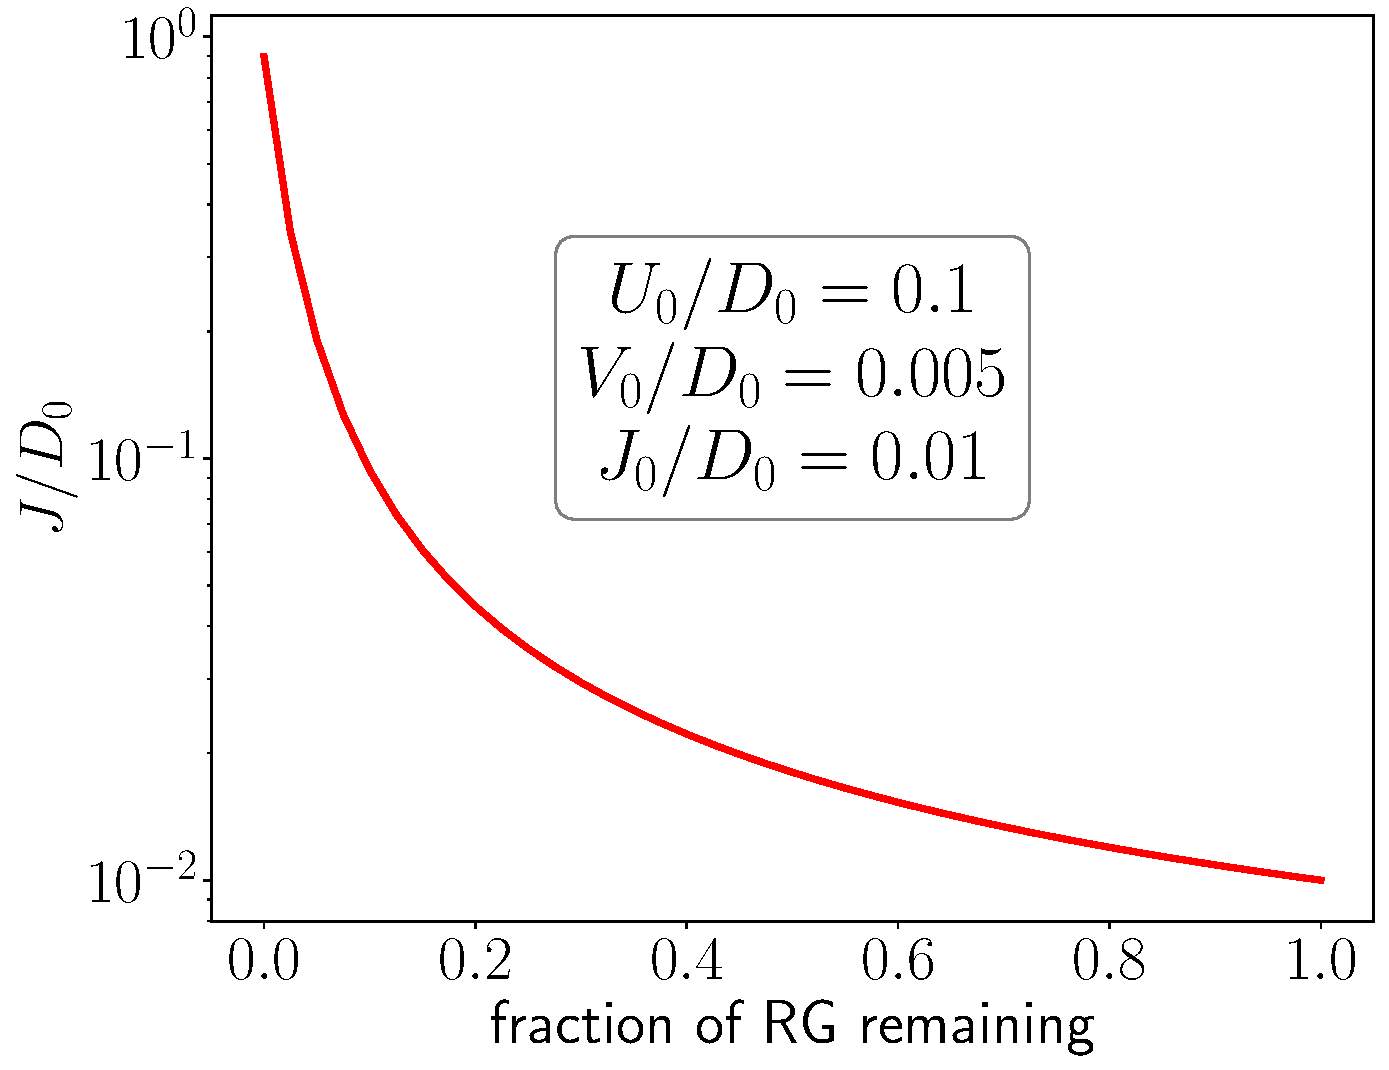
\includegraphics[width=0.32\textwidth]{../figures/U_rel,U>0,J.pdf}
%\end{figure}

\begin{figure}[htpb]
	\centering
	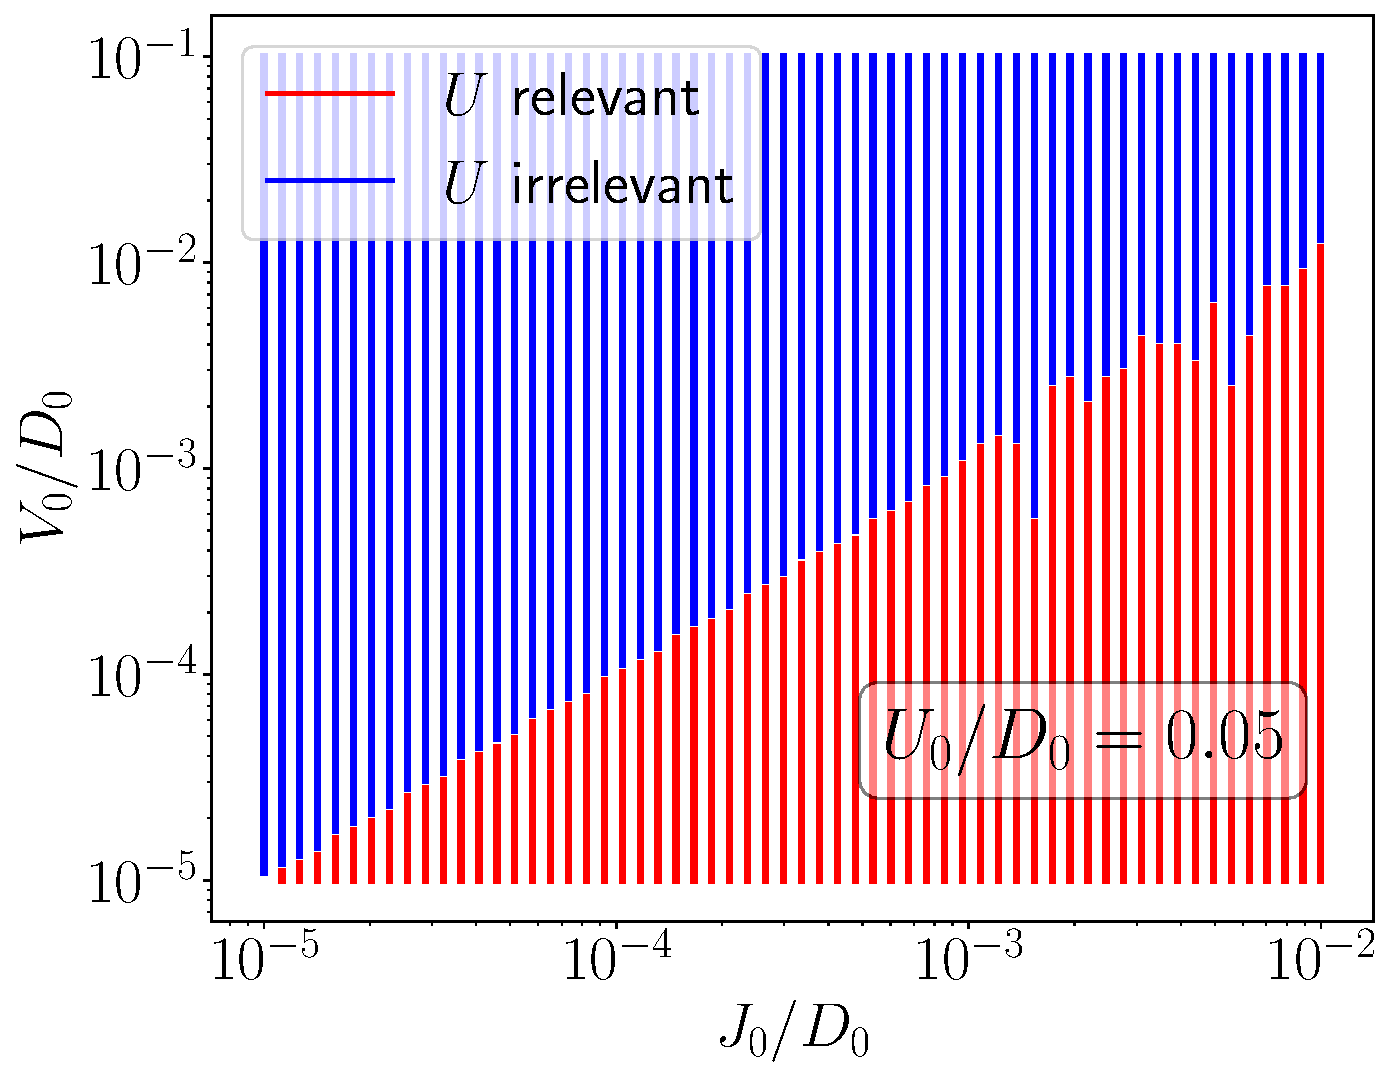
\includegraphics[width=0.48\textwidth]{../figures/VvsJ_relvsirr.pdf}
	\hspace*{\fill}
	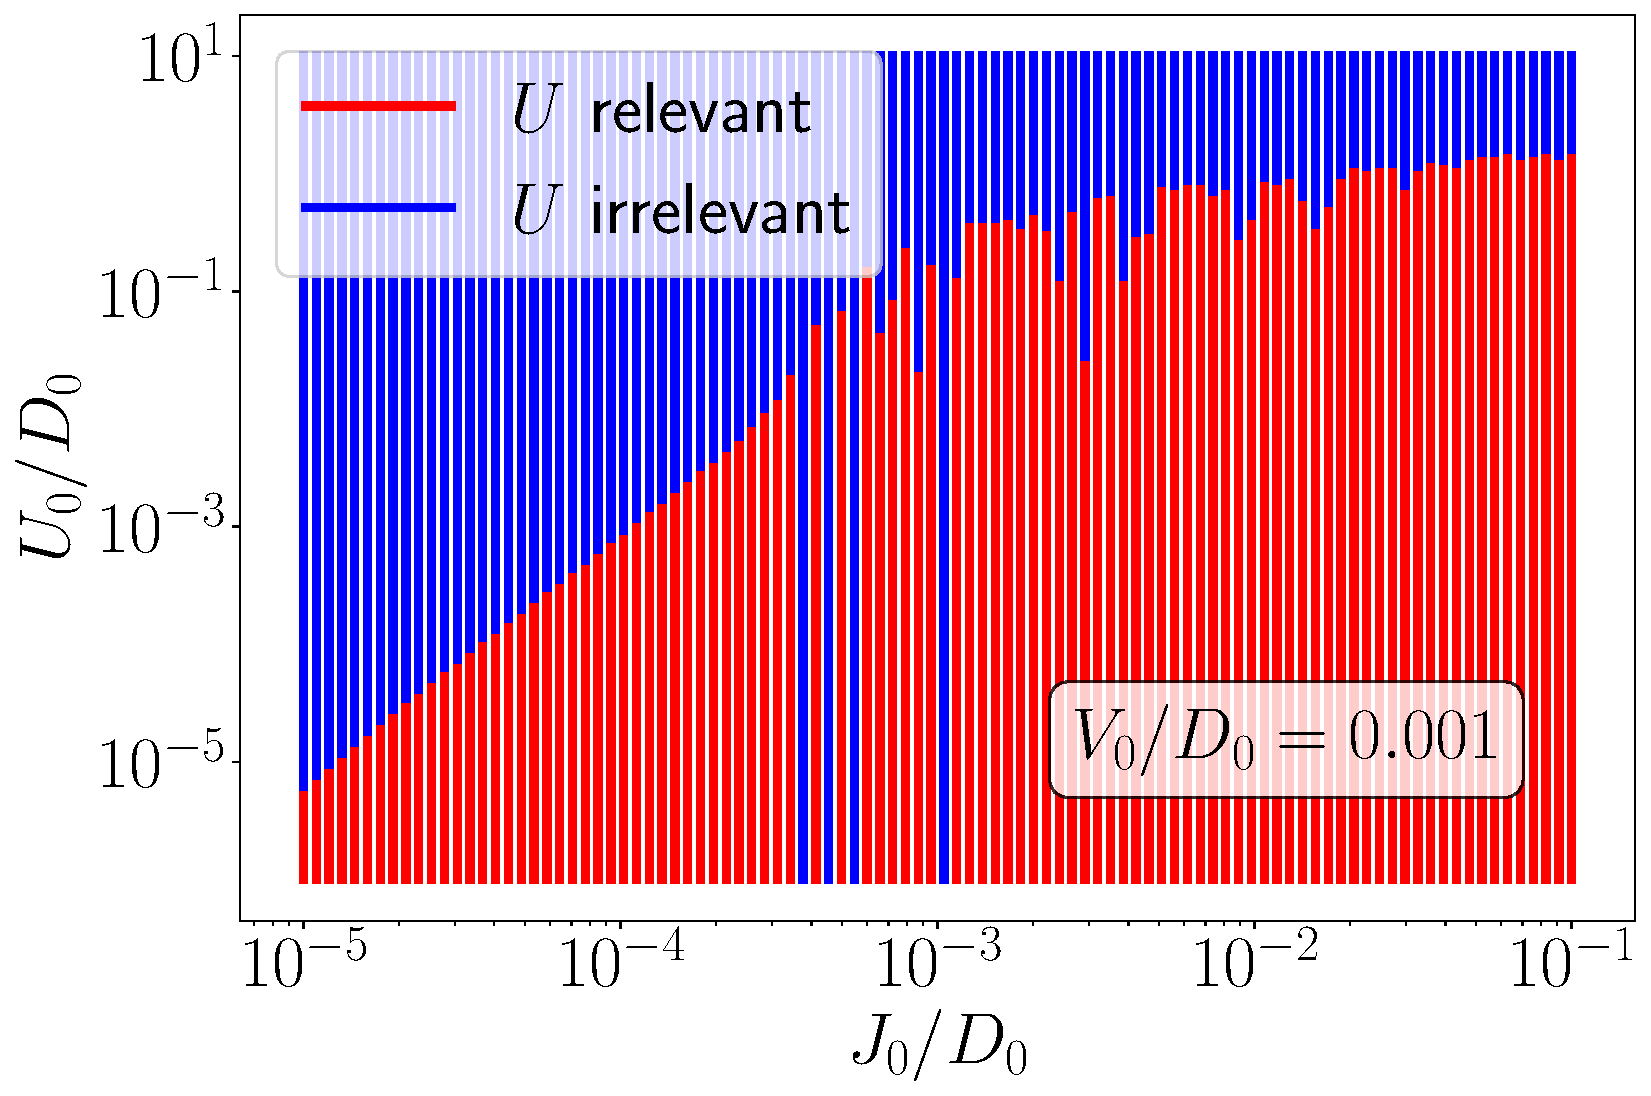
\includegraphics[width=0.48\textwidth]{../figures/UvsJ_relvsirr.pdf}
\end{figure}

\begin{figure}[htpb]
	\centering
	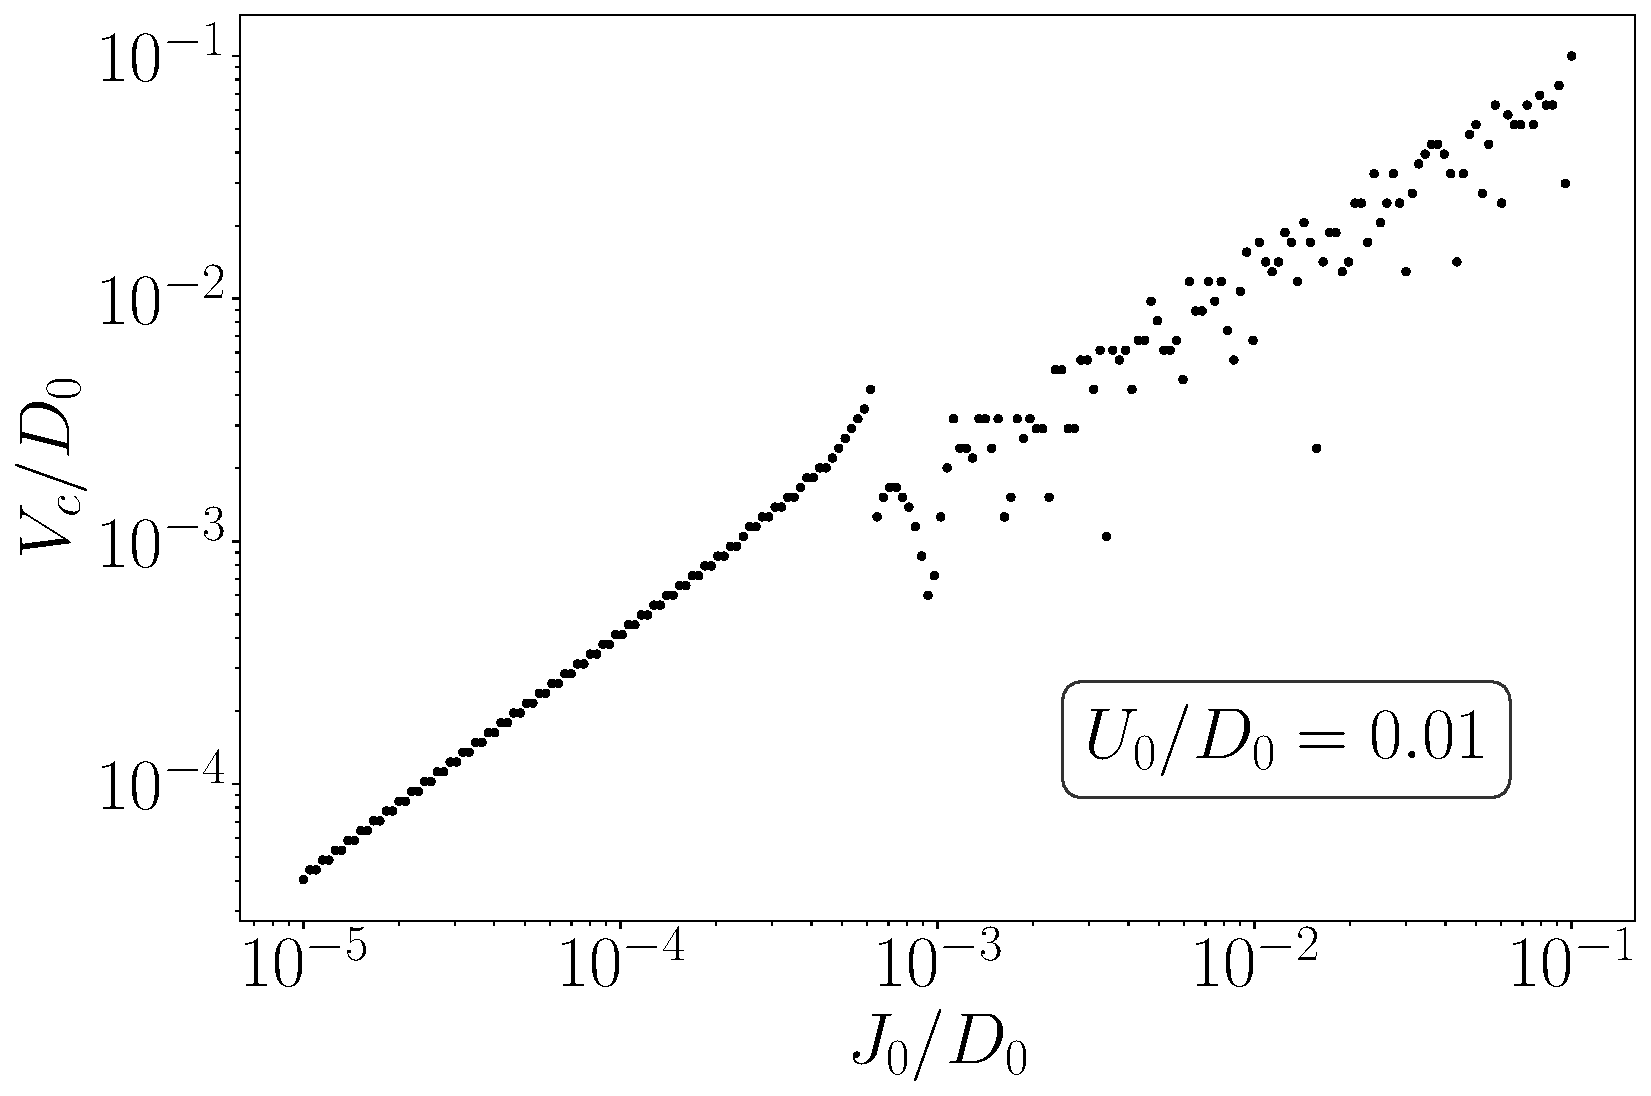
\includegraphics[width=0.48\textwidth]{../figures/VcvsJ.pdf}
	\hspace*{\fill}
	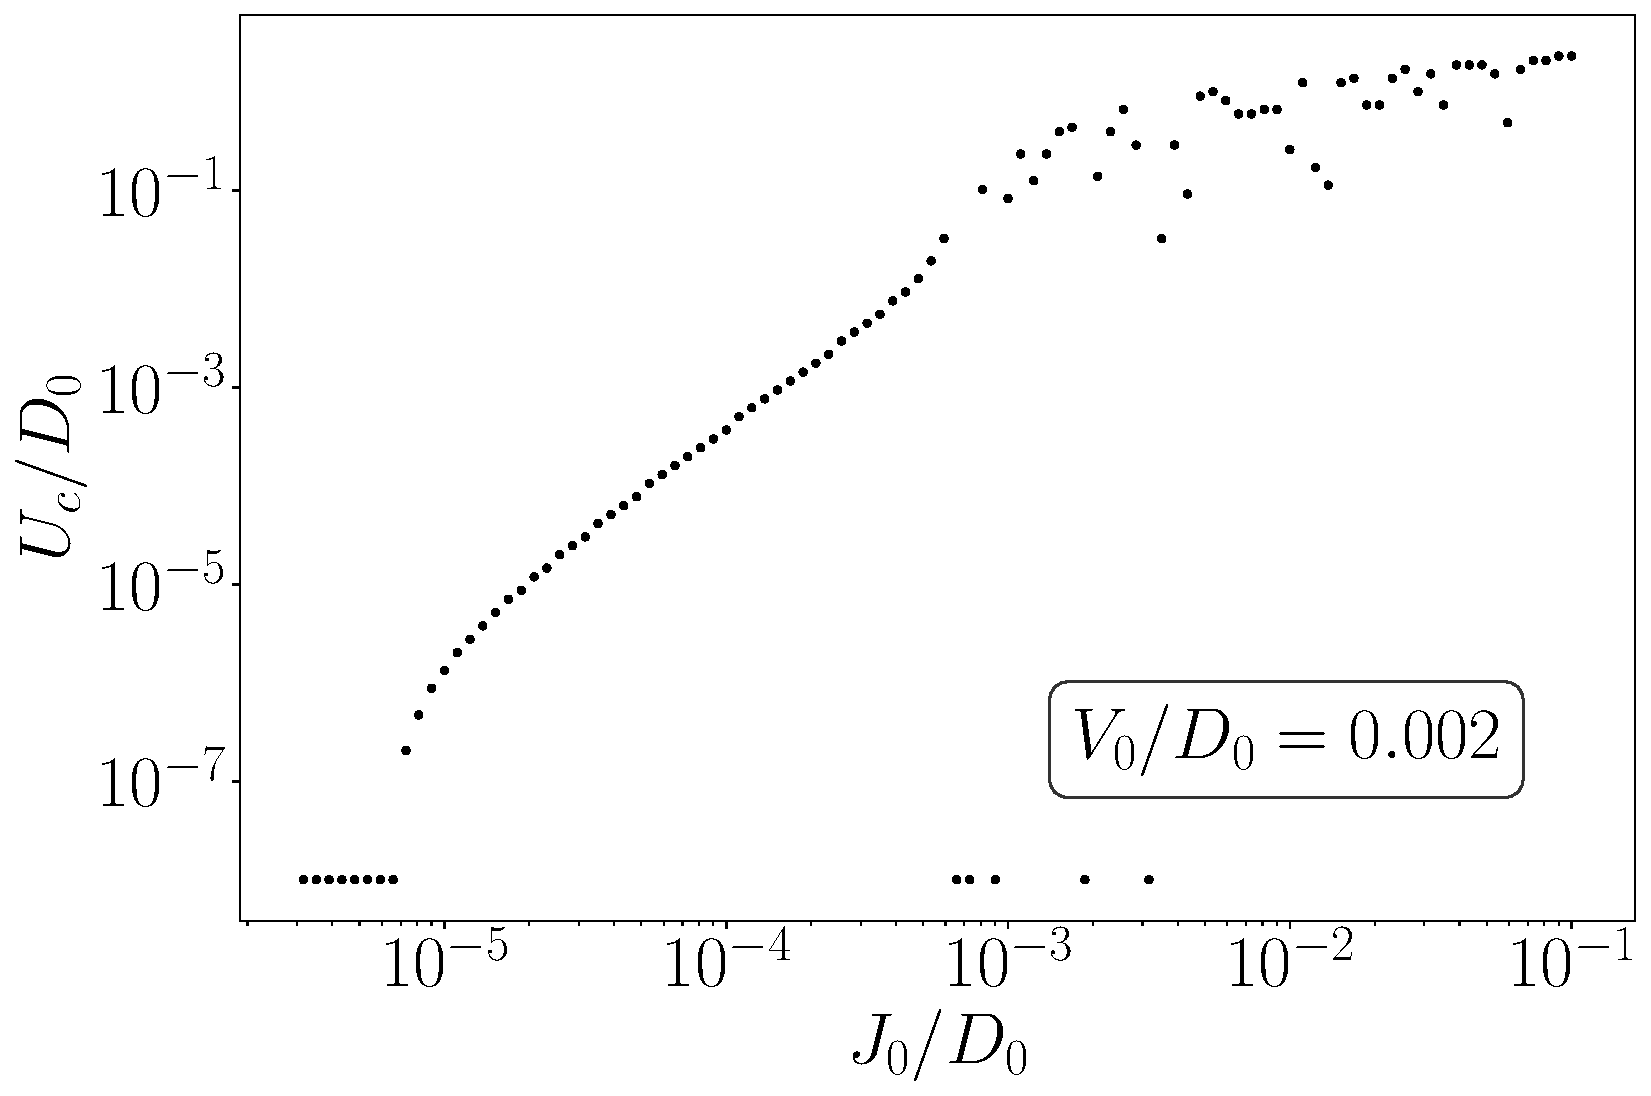
\includegraphics[width=0.48\textwidth]{../figures/UcvsJ.pdf}
\end{figure}

\subsection{Attractive interaction on impurity: \(U<0\)}
Here, we have \(J<0\) and \(K>0\). The denominators satisfy the following inequality in this regime:
\begin{equation}\begin{aligned}
	d_0 > d_3 > d_2 > d_1
\end{aligned}\end{equation}

The strong-coupling regime here corresponds to \(d_0 < 0\). This again means that all the denominators are negative. The spin-exchange coupling \(J\) is now irrelevant, because its bare value is negative while its RG equation is positive: \(\Delta J>0\). Moreover, the isospin coupling \(K\) is now positive and so is its RG equation: \(\Delta K>0\), which means it flows to strong-coupling. \(V\) also flows to strong-coupling. The RG equation for \(U\) can be written as
\begin{equation}\begin{aligned}
	\Delta U = 4V^2\left(\frac{K}{4} - U\right)\frac{n_j}{d_0 d_1} + \frac{n_j K^2}{d_3}
\end{aligned}\end{equation}
The first term is necessarily positive, while the second term is negative. This means that for roughly \(V_0 > J_0\), we  will have \(\Delta U > 0\), and since \(U_0 < 0\), this amounts to an irrelevant flow of \(U\) towards zero. On the other hand, for \(J_0 > V_0\), we will have \(\Delta U < 0\), and this corresponds to a relevant flow of \(U\) towards large negative value.

In other words, the RG flows in this regime can be exactly mapped to those in the positive \(U\) regime. The general statement is: in the strong-coupling regime of positive(negative) \(U\), \(V\) is always relevant, \(J\)(\(K\)) is relevant, \(K\)(\(J\)) is irrelevant, and \(U\) is relevant when \(J(K) > V\), otherwise \(U\) is irrelevant.


\section{Effective Hamiltonian and ground state}
The fixed point Hamiltonian can, in general, be written as
\begin{equation}\begin{aligned}
	\mathcal{H}^* = \sum_{\sigma, k}\epsilon_k \tau_{k\sigma} - \frac{U^*}{2}\left(\hat n_{d \uparrow} - \hat n_{d \downarrow}\right)^2  + \sum_{\sigma, k < \Lambda^*}\left( V^* c^\dagger_{k\sigma}c_{d\sigma} + \text{h.c.} \right) + J^* \vec{S_d}\cdot\vec{s} + K^* \vec{C_d}\cdot\vec{C}
\end{aligned}\end{equation}
The first term is the kinetic energy of all the electrons. The next two terms are the impurity-diagonal pieces, featuring the renormalised interaction \(U^*\). The next three terms are the residual interactions between the impurity and the metal, with the renormalised couplings \(V^*, J^*\) and \(K^*\). The summations in these terms extend from the fixed point momentum cutoff \(\Lambda^*\) to 0. This is the region of momentum space  which the URG was unable to decouple. The operators \(\vec s\) and \(\vec C\) represent the macroscopic magnetic and charge spins formed by the remaining electrons that are lying inside the window \(\left[ 0, \Lambda^* \right] \):
\begin{equation}\begin{aligned}
	\vec s = \sum_{kk^\prime<\Lambda^*\atop{\alpha\beta}} c^\dagger_{k\alpha}\vec \sigma_{\alpha\beta}c_{k^\prime\beta}
\end{aligned}\end{equation}
Our goal here is to write down the ground state wavefunction for this low-energy Hamiltonian.

To make progress, we will simplify the effective Hamiltonian by taking the zero bandwidth limit. This reduces it to a two-site problem. One site is of course the impurity site, and this site will be labeled as site 1. The other site will be formed by the center of mass degree of freedom of the conduction electrons, and will be labeled as site 2. The Hamiltonian for this two-site problem is
\begin{equation}\begin{aligned}
	\mathcal{H}_{IR} = - \frac{U^*}{2}\left(\hat n_{1 \uparrow} - \hat n_{1 \downarrow}\right)^2 + V^*\sum_{\sigma}\left(c^\dagger_{1\sigma}c_{2\sigma} + \text{h.c.} \right) + J^*\vec{S_1}\cdot\vec{S_2} + K^* \vec{C_1}\cdot\vec{C_2}
\end{aligned}\end{equation}
\begin{figure}[!htb]
	\centering
	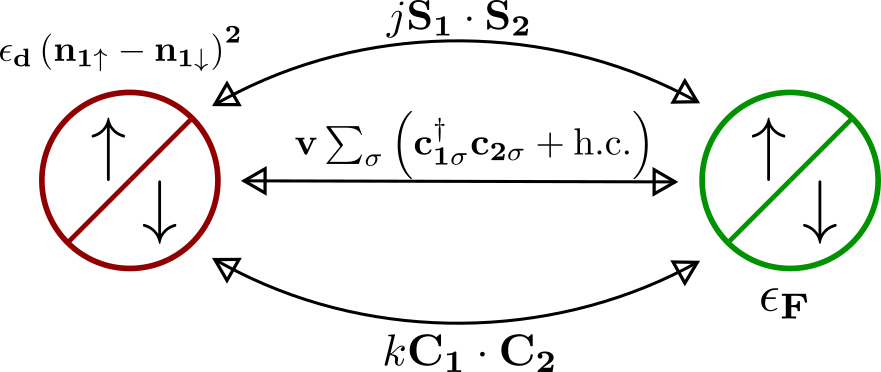
\includegraphics[width=0.4\textwidth]{../figures/two_site_problem.png}
	\caption{Two-site effective problem of fixed point Hamiltonian}
	\label{twosite}

\end{figure}
The subscripts on the operators designate the site on which they act; \(\hat n_1\) is the number operator for the first site.

We will adopt the following notation to represent the states in this Hilbert space. A general state will be represented in the Fock space basis as \(\ket{n_{1 \uparrow}n_{1 \downarrow}n_{2 \uparrow}n_{2 \downarrow}}\). For example,
\begin{equation}\begin{aligned}
	\ket{1101} = c^\dagger_{1 \uparrow}c^\dagger_{1 \downarrow}c^\dagger_{2 \downarrow}\ket{-}
\end{aligned}\end{equation}
\(\ket{-}\) is the vacuum state.

For \(U>0\), the ground state is given by
\begin{gather}
	\label{gstate}
	\ket{\Psi}_\text{1} = c_s \frac{1}{\sqrt 2}\left(\ket{\uparrow, \downarrow} - \ket{\downarrow, \uparrow}\right) + c_c \frac{1}{\sqrt 2}\left(\ket{\uparrow\downarrow, 0} + \ket{0, \uparrow\downarrow}\right), \quad E_1 =  -V^*\sqrt{\gamma^2 + 4} -\frac{1}{4}U^* - \frac{3}{8}{J^*}
\end{gather}
where $\gamma = \frac{1}{2{V^*}}\left[ \frac{1}{4}\left( 3J^* + K^* \right) + \frac{1}{2}U^* \right]$. The probabilities for the spin and charge sectors for the ground state are
\begin{equation}\begin{aligned}
	\label{coeff_def}
	\left(c_s\right)^2 = \frac{1}{2\sqrt{\gamma^2 + 4}}\left(\sqrt{\gamma^2 + 4} + \gamma\right), \quad \left(c_c \right)^2 = \frac{1}{2\sqrt{\gamma^2 + 4}}\left(\sqrt{\gamma^2 + 4} - \gamma\right)~.
\end{aligned}\end{equation}
For (roughly) \(J_0 > V_0\), we get \(J^* \gg V^*\) and \(U^* \gg U_0\) so that \(\gamma \gg 1\). This gives \(\left( c_s \right) ^2 \sim 1\) and \(\left( c_c \right) ^2 \sim 0\). The entire contribution to the ground state then comes from the spin sectors of the two sites. This is calculated numerically in fig.~\ref{cs_cc}.
\begin{figure}[htpb]
	\centering
	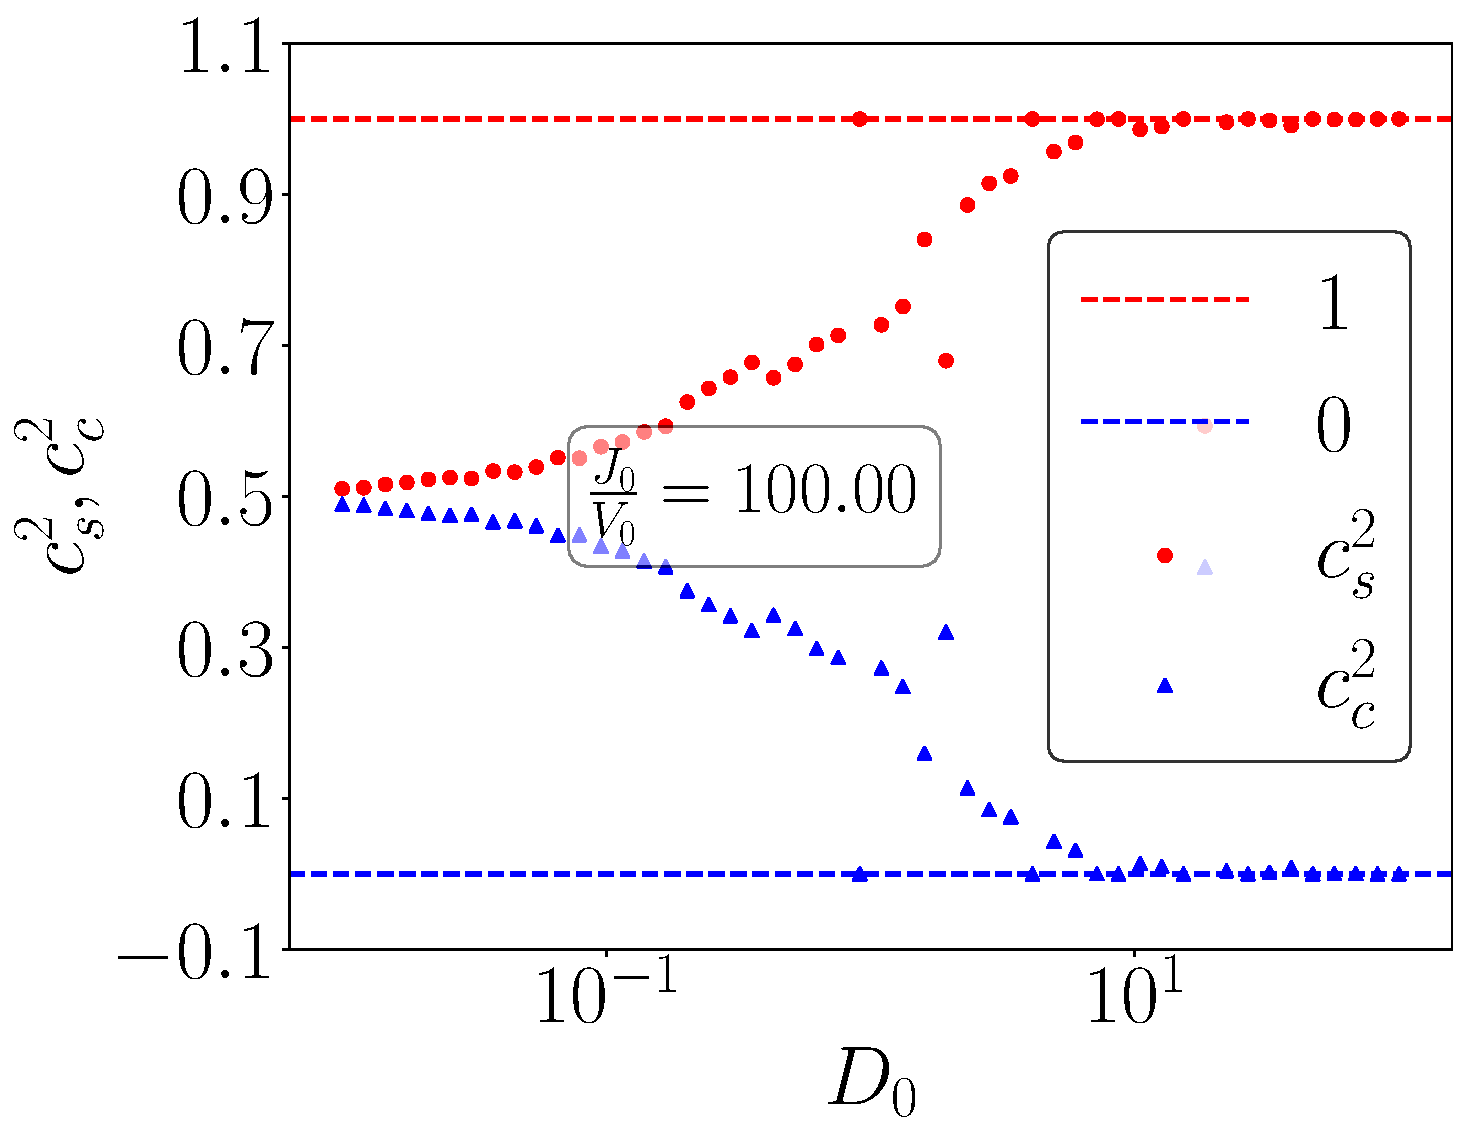
\includegraphics[width=0.8\textwidth]{../figures/coeffs_vs_J.pdf}
	\caption{Variation of relative weights \(c_s\) and \(c_c\) with \(J_0\)}
	\label{cs_cc}
\end{figure}

In the other regime of \(U<0\), the two competing states are \(\ket{\Psi}_1\) defined above (with energy \(E_1\)), and \(\ket{\Psi_2}\), the charge singlet: \(\ket{\Psi}_2 = \frac{1}{\sqrt 2}\left( \ket{2,0} - \ket{0,2} \right)\) having energy \(E_2\).
\begin{equation}\begin{aligned}
	E_2 = -\frac{3}{4}K^*, \quad E_1 - E_2 = -\frac{1}{4}\sqrt{\left( \frac{1}{2}K^* + U^* \right)^2 + (4V^*)^2} - \frac{1}{4}U^* + \frac{3}{4}K^*
\end{aligned}\end{equation}
For \(V_0 \gg K_0\), the largest energy scale will be \(V^*\), and we can then approximate this difference as
\begin{equation}\begin{aligned}
	E_1 - E_2 \simeq -V^* < 0
\end{aligned}\end{equation}
In such a case, \(\ket{\Psi}_1\) will therefore be the ground state. In the other regime \(V_0 \ll K_0\), the largest energy scale will be \(K^*\), and we can then write
\begin{equation}\begin{aligned}
	E_1 - E_2 \simeq - \frac{1}{8}K^* + \frac{3}{4}K^* > 0
\end{aligned}\end{equation}
In this case, the ground state will be \(\ket{\Psi}_2\). There exists, therefore, a phase transition at a critical plane \((U_c, K_c, V_c)\), where the ground state changes between the charge singlet \(\ket{\Psi}_2\) and the spin singlet + charge triplet \(\ket{\Psi}_1\).

\section{Approach towards the thermodynamic limit}
The URG method works strictly on finite systems and leads to finite values of fixed point couplings. The behaviour of the Hamiltonian in the thermodynamic limit can then be determined using finite-size scaling where we increase the bandwidth and decrease the width of each RG step. When applied to the fixed point value of the impurity-bath hybridisation parameter \(V\) (fig.~\ref{V_vs_D}), it can be seen that the fixed point value increases as the system size is increased, implying that the continuum limit of \(V^*\) is \(\infty\). This holds for both \(V_0 > J_0\) and \(V_0 < J_0\), as shown in the two panels of fig.~\ref{V_vs_D}.
\begin{figure}[htpb]
	\centering
	\hspace*{\fill}
	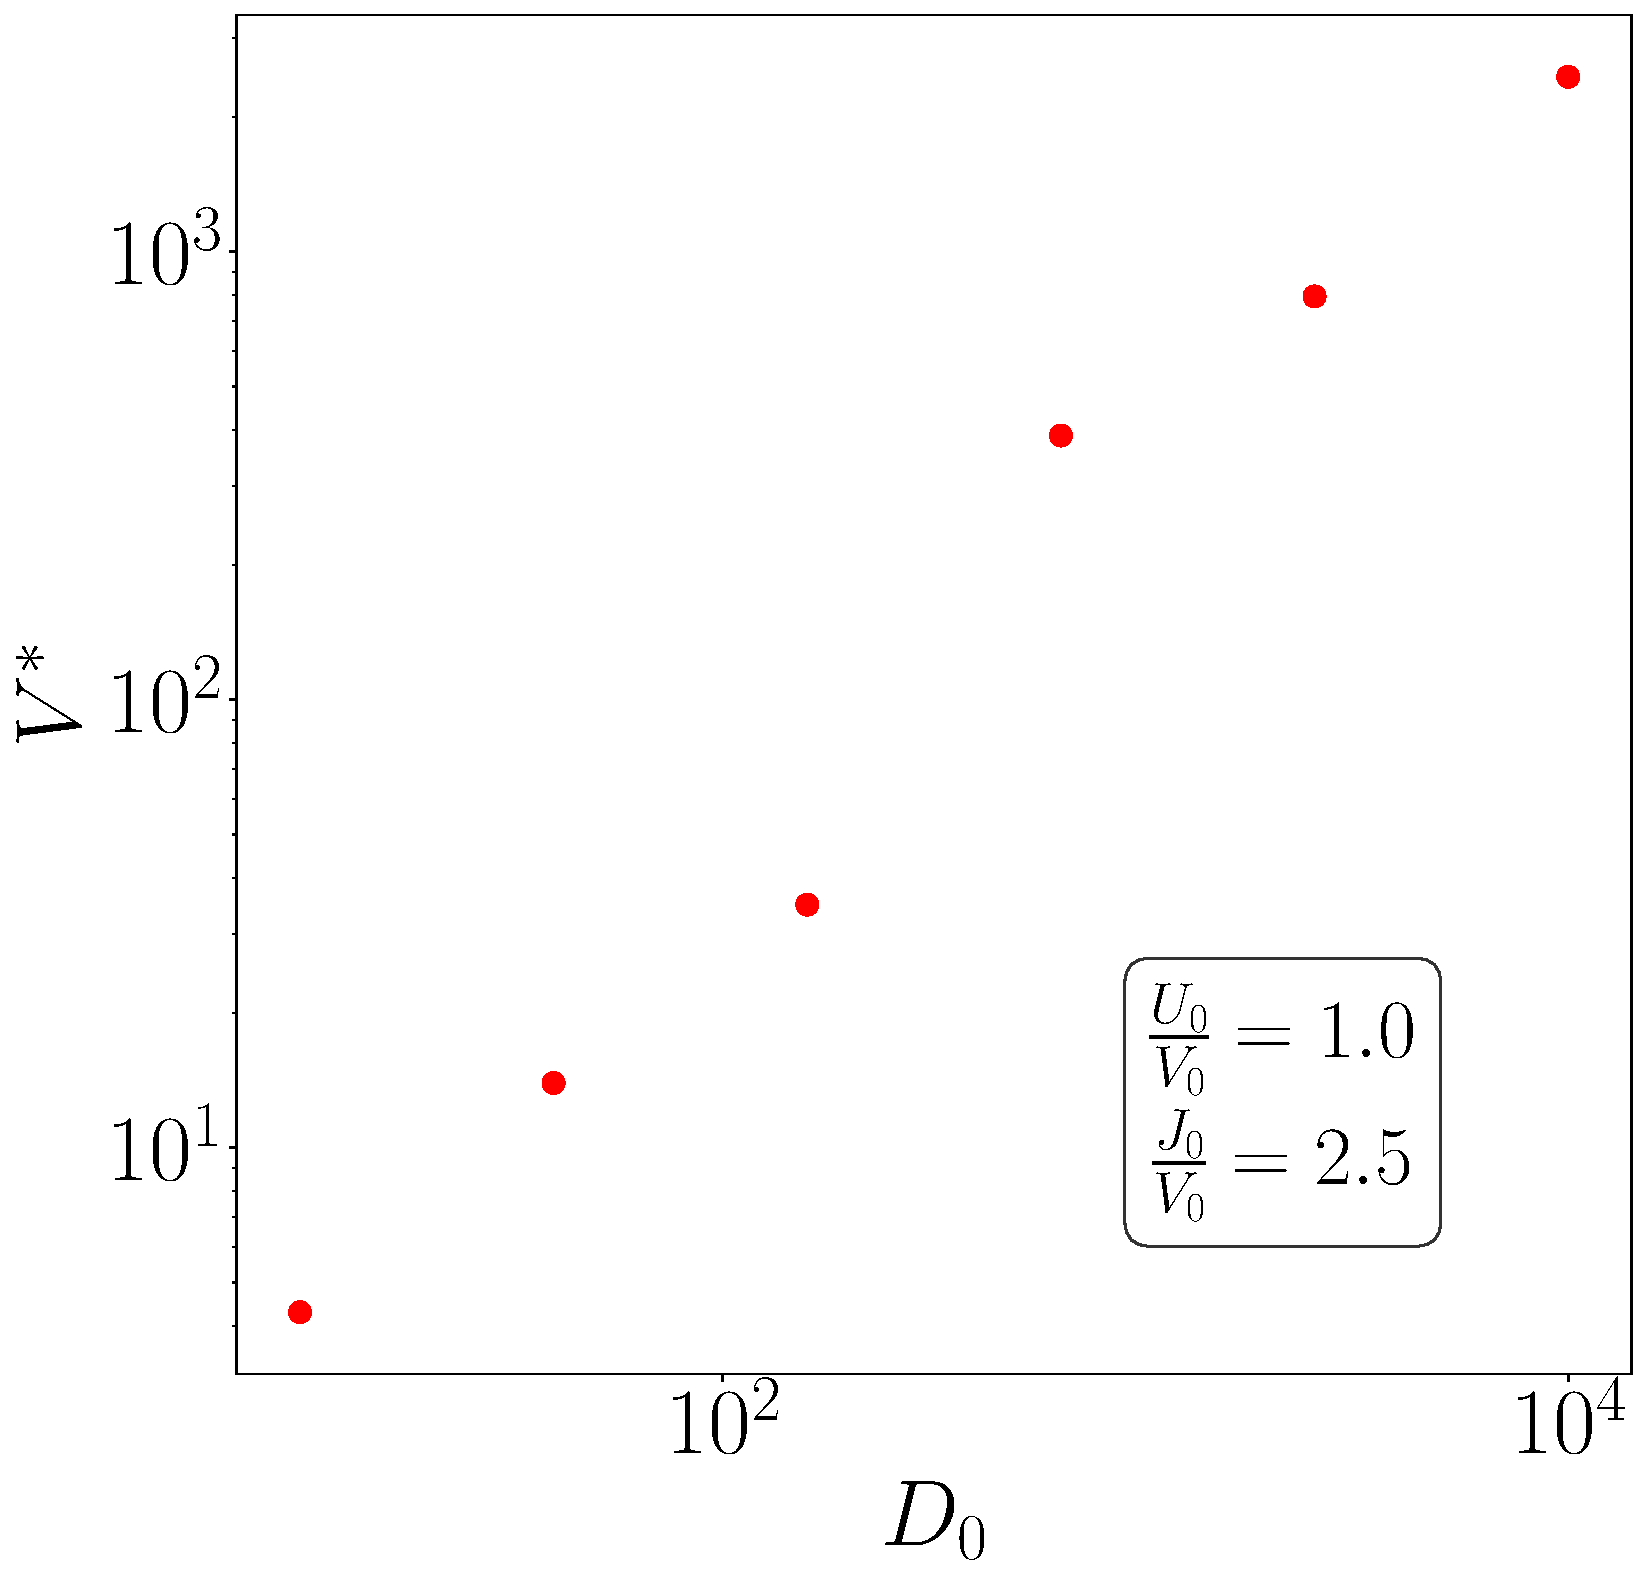
\includegraphics[width=0.4\textwidth]{../figures/Vstar_vs_D_smallV.pdf}
	\hspace*{\fill}
	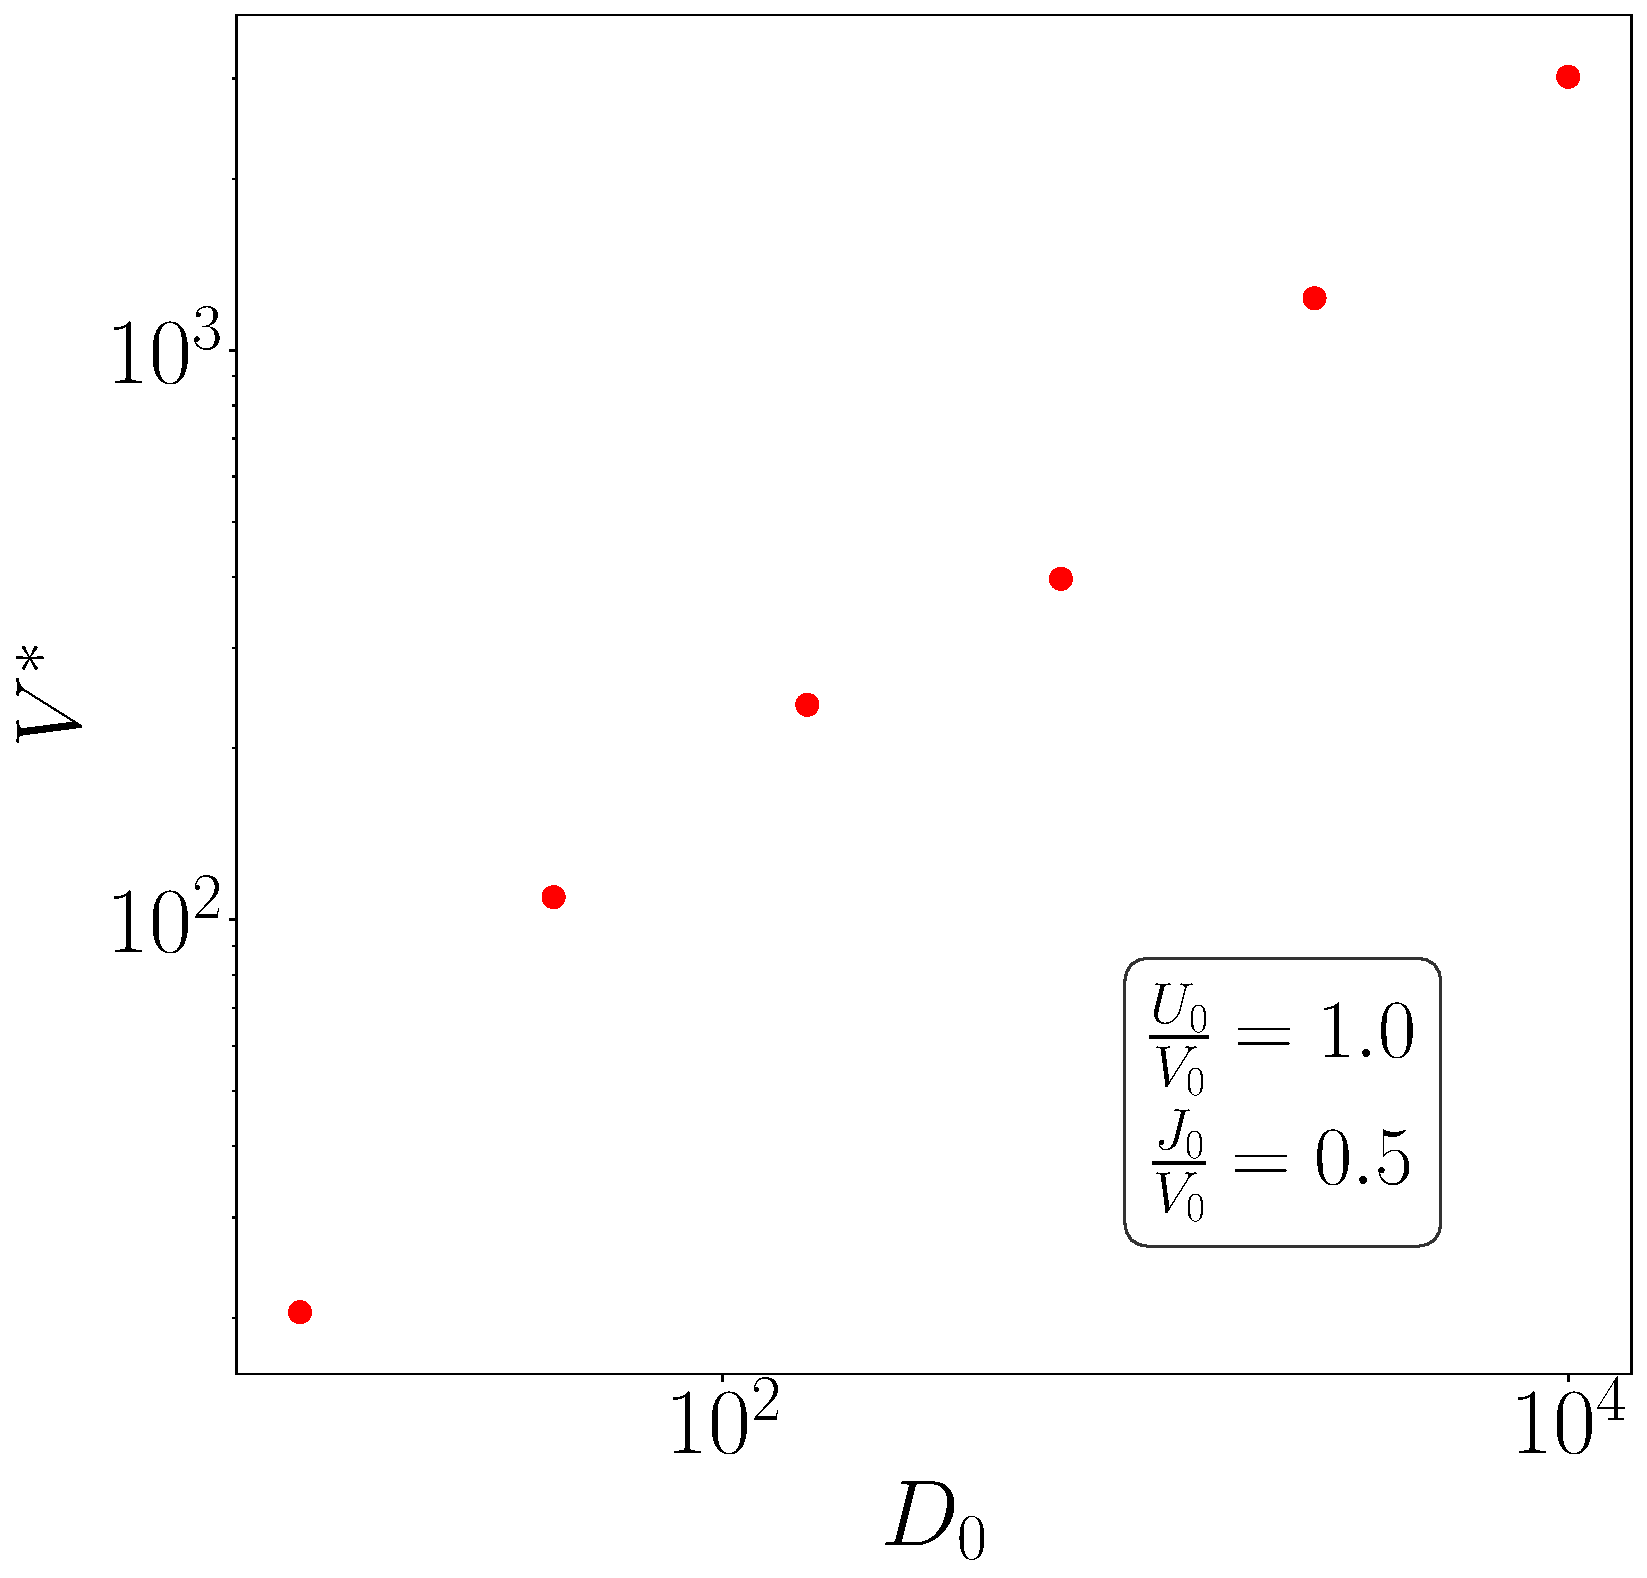
\includegraphics[width=0.4\textwidth]{../figures/Vstar_vs_D_largeV.pdf}
	\hspace*{\fill}
	\caption{Variation of fixed point value \(V^*\) with increasing bandwith \(D_0\), for both \(V_0 > J_0\) and \(V_0 < J_0\).}
	\label{V_vs_D}
\end{figure}

In a similar manner, we checked the variation of the spin and charge probabilities, \(c_s\) and \(c_c\), in the ground state, with increasing bandwith. The result is shown in fig.~\ref{c_vs_D}.
\begin{figure}[htpb]
	\centering
	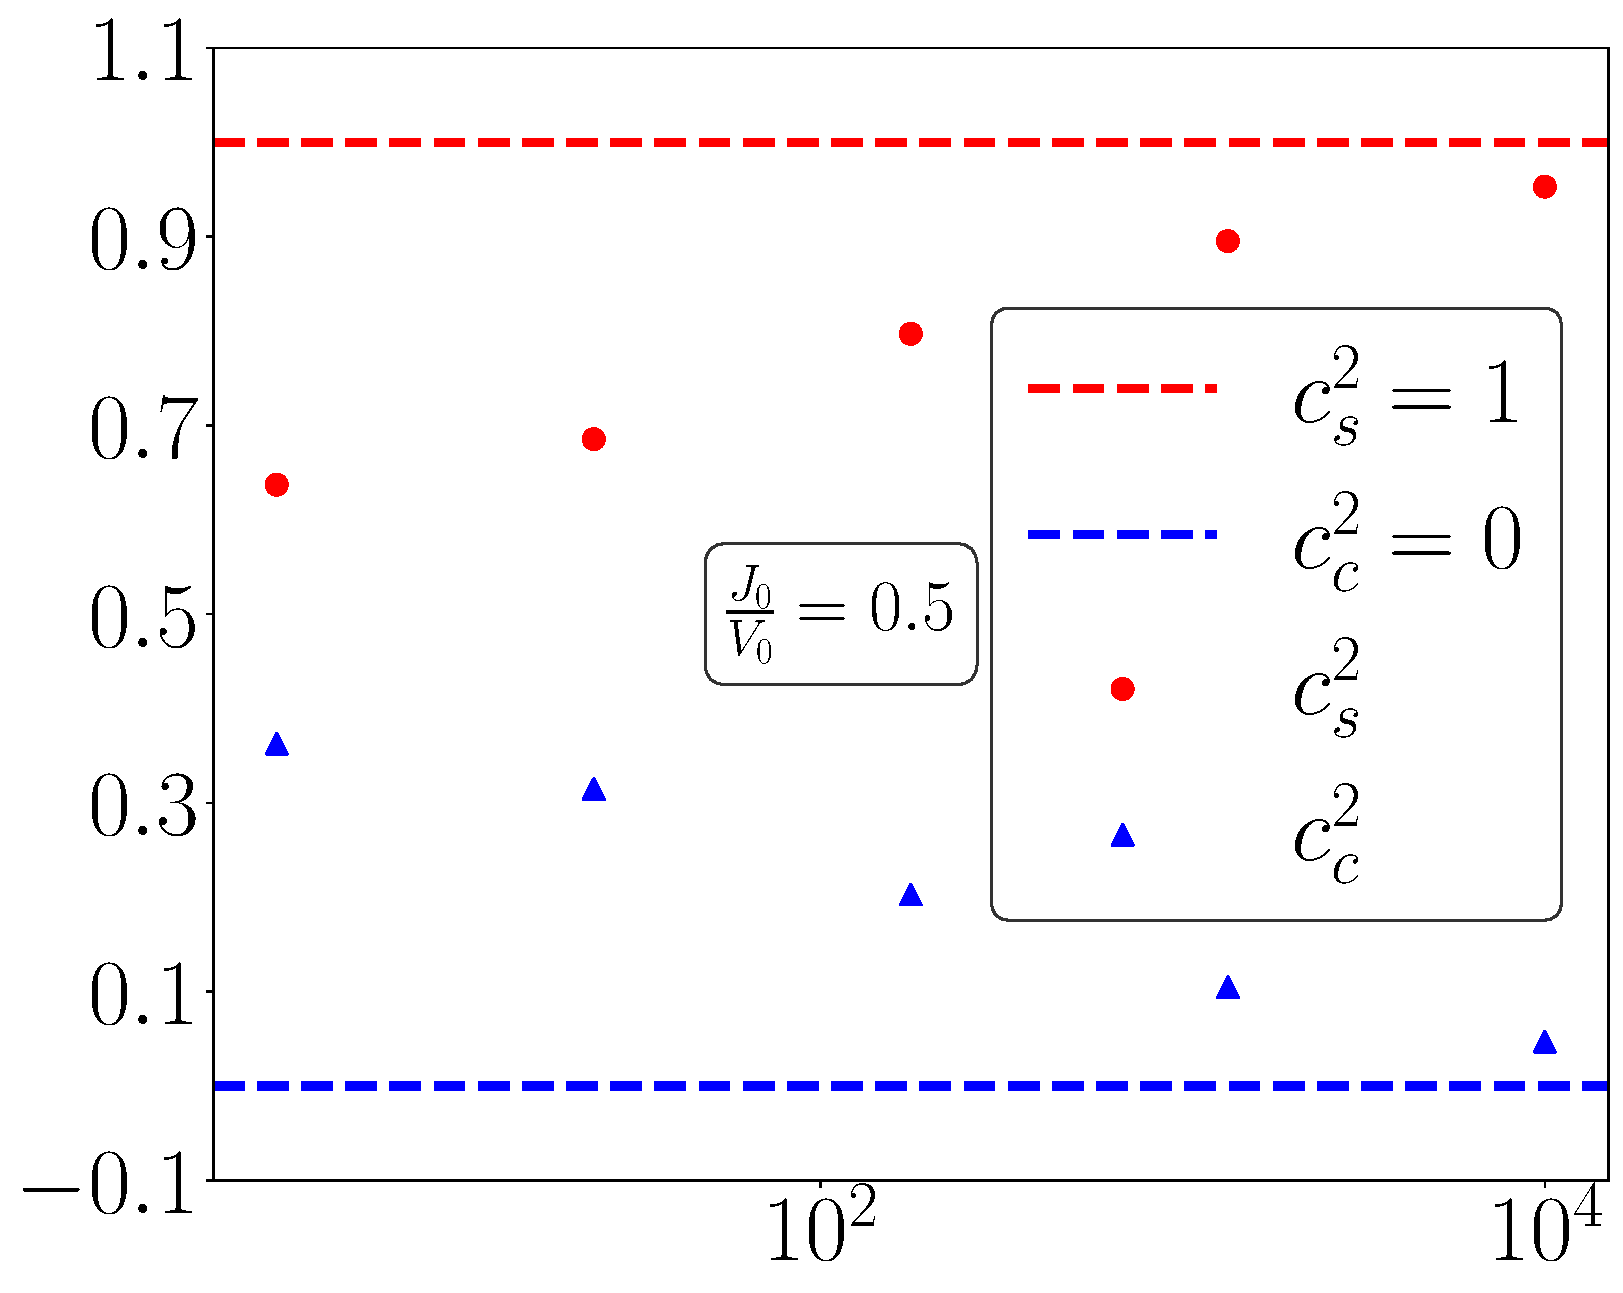
\includegraphics[width=0.45\textwidth]{../figures/coeffs_vs_D_largeV.pdf}
	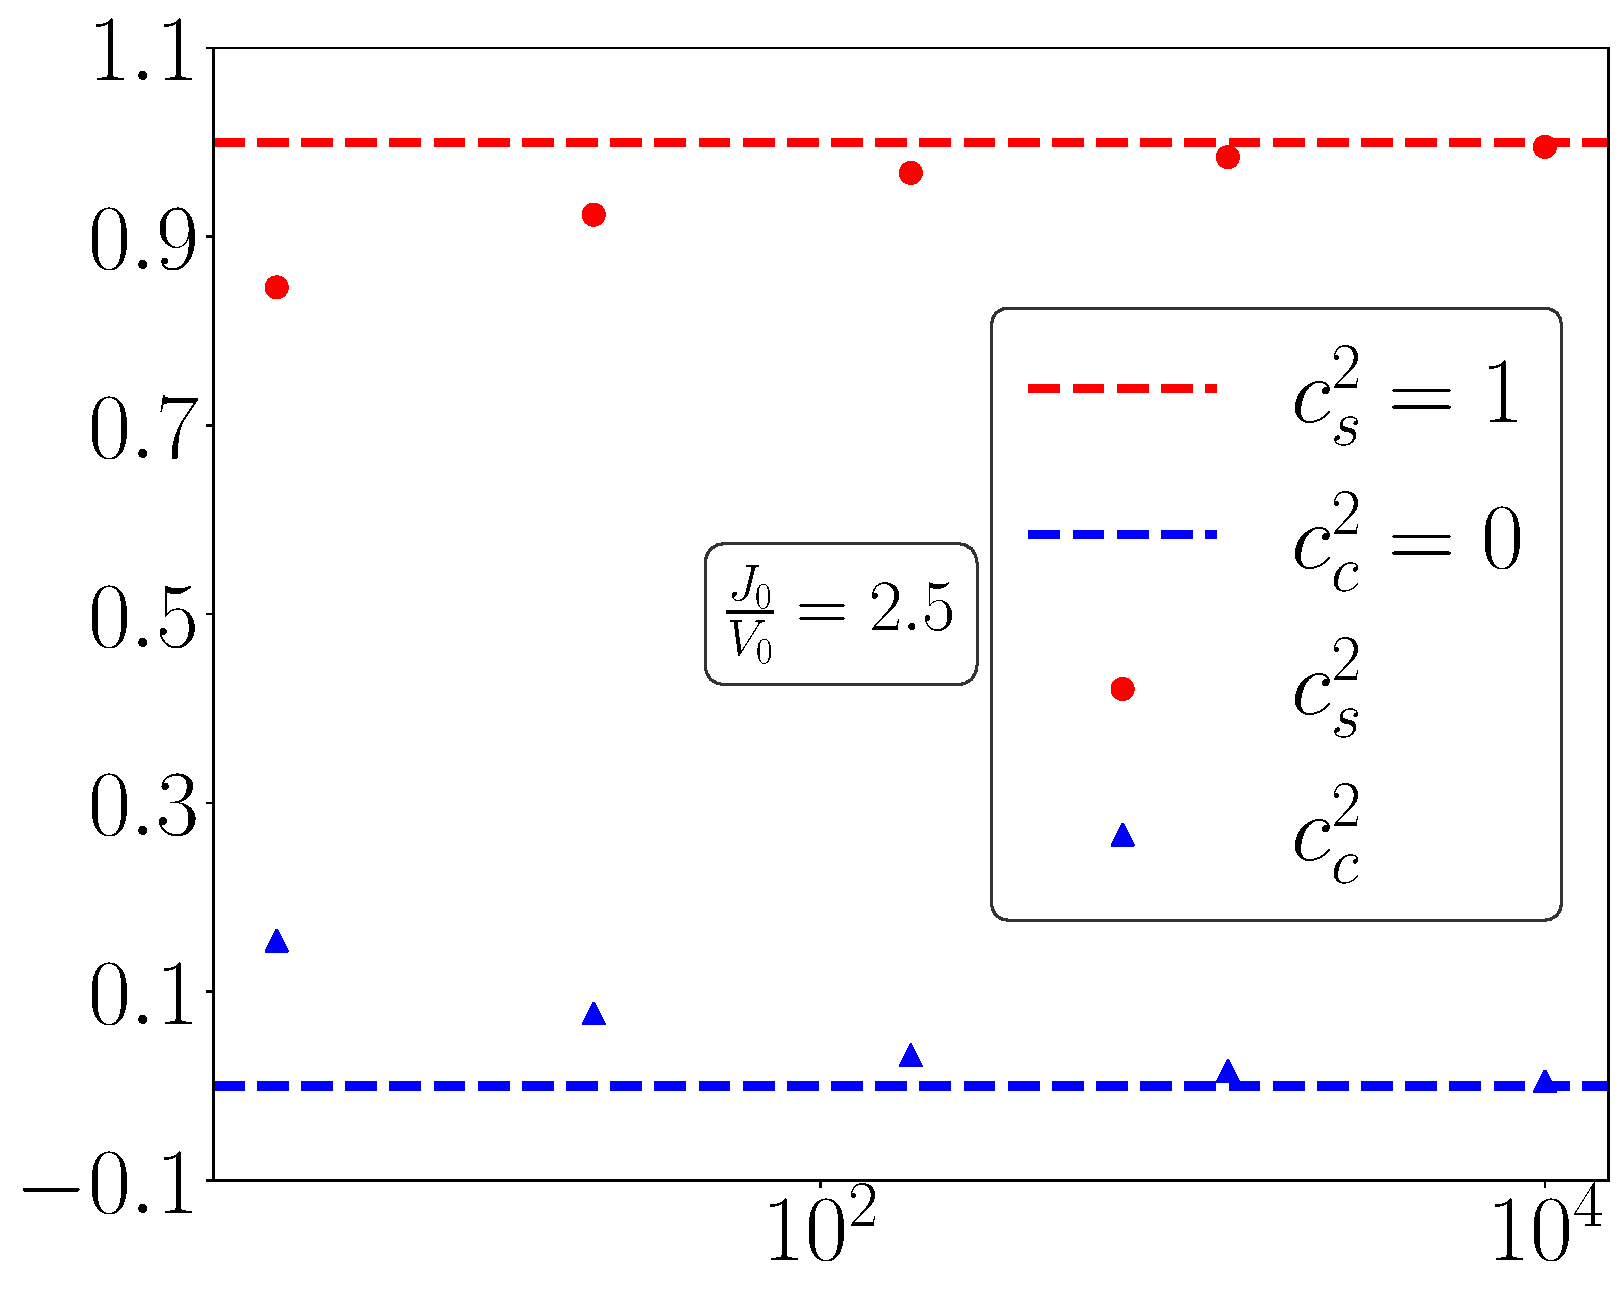
\includegraphics[width=0.45\textwidth]{../figures/coeffs_vs_D_smallV.pdf}
	\caption{Variation of spin and charge fractions, \(c_s\) and \(c_c\), of the ground state, as a function of bare bandwidth \(D_0\). Left and right panels show the cases of \(J_0 < V_0\) and \(J_0 > V_0\) respectively.}
	\label{c_vs_D}
\end{figure}
For both \(V_0 < J_0\) and \(V_0 > J_0\), we see that the spin contribution increases towards unity while the charge contribution vanishes. This indicates that at large bandwidth, the ground state becomes purely a spin singlet, formed purely by singly-occupied impurity states.
\begin{equation}\begin{aligned}
	\label{gstate_kondo}
	\lim_{D_0 \to \infty} \ket{\Psi}_1 = \frac{1}{\sqrt 2}\left(\ket{\uparrow, \downarrow} - \ket{\downarrow, \uparrow}\right) 
\end{aligned}\end{equation}

\section{Effective temperature scale at the fixed point}
We will first change the discrete RG equation to a continuum equation by interpreting \(\Delta J\) as \(\frac{\Delta J}{\Delta \ln D}\), where the denominator is unity: \(\Delta \ln D = 1\). Now, since the bandwidth is decreasing under the RG, we can write \(\Delta \ln D = -d \ln D\). The continuum equation (for \(K=0\)) becomes
\begin{equation}\begin{aligned}
	\frac{\:\mathrm{d}J}{\:\mathrm{d}\ln D} = n(0)J^2 \frac{1}{\omega - \frac{D}{2} + \frac{J}{4}}
\end{aligned}\end{equation}
where we have replaced by the number of states at each shell with that at the Fermi surface (uniform DOS). We can define a dimensionless quantity \(g \equiv \frac{J}{\frac{D}{2}} - \omega\). In terms of \(g\), the continuum RG equation becomes
\begin{equation}\begin{aligned}
	-\frac{\:\mathrm{d}g}{\:\mathrm{d}\ln D} + \frac{D g}{2\omega - D} = \frac{n(0) g^2}{1 - \frac{g}{4}}
\end{aligned}\end{equation}
Now, for the specific case where \(D\) is small (\(D \to 0\)), we can simplify and integrate this equation:
\begin{equation}\begin{aligned}
	\frac{\:\mathrm{d}g}{\:\mathrm{d}\ln D} &= \frac{n(0) g^2}{\frac{g}{4} - 1}\\
	\implies \left[\frac{1}{g} + \frac{1}{4}\ln g\right]_{g_0}^{g^*} &= n(0)\ln D\big\vert_{D_0}^{D^*}
\end{aligned}\end{equation}
\(g^*(_0), D^*(_0)\) are the fixed point (bare) values of \(g, D\). From the denominator structure, the fixed-point value is \(g^* =  4\). This gives an estimate of the bandwidth of the emergent window:
\begin{equation}\begin{aligned}
	D^* = D_0 \left( \frac{4}{g_0} \right)^\frac{1}{4n(0)}\exp\left\{-\frac{1}{n(0)}\left(\frac{1}{g_0} - \frac{1}{4}\right)\right\}
\end{aligned}\end{equation}
We can now define a temperature scale for the fixed-point theory:
\begin{equation}\begin{aligned}
	T_K \equiv \frac{2N^*}{\pi}D^* = \frac{2N^*}{\pi}D_0 \left( \frac{4}{g_0} \right)^\frac{1}{4n(0)}\exp\left\{-\frac{1}{n(0)}\left(\frac{1}{g_0} - \frac{1}{4}\right)\right\}
\end{aligned}\end{equation}
The factor of \(2N^*\) is inserted to make the Kondo temperature intensive (we will see below that the \(N^*\) allows it to  be written in terms of parameters of the two-site Hamiltonian) - \(2N^*\) is the total number of momentum states in the fixed point theory. The factor of \(\frac{1}{\pi}\) is for aesthetic reasons. Since we have and will primarily work with \(\omega=0\), the fixed point condition can be used to write \(D^* = \frac{J^* + K^*}{2}\).
\begin{equation}\begin{aligned}
	T_K = \frac{2N^*}{\pi}\frac{1}{2}\left(J^* + K^*\right) = \frac{1}{\pi}\left(j + k\right)
\end{aligned}\end{equation}
\section{Impurity susceptibilities}
\subsection{Spin susceptibility}
The spin susceptibility is defined as
\begin{equation}\begin{aligned}
	\label{chi_def}
	\chi(\beta) = \beta \left(\left<\left(S_d^z\right)^2\right> - \left<S_d^z\right>^2\right)
\end{aligned}\end{equation}
There is an alternate way of calculating this. We insert a fictitious magnetic field that couples only to the impurity site. The Hamiltonian in the presence of this field is
\begin{equation}\begin{aligned}
	\label{field_ham}
	\mathcal{H}^\prime(B) = \mathcal{H} + B S_d^z
\end{aligned}\end{equation}
The susceptibility is then given by
\begin{equation}\begin{aligned}
	\label{chi_exp}
	\chi(\beta) &= \lim_{B \to 0}\frac{1}{\beta}\left[\frac{1}{Z(B)} \frac{\partial^2{Z(B)}}{\partial{B^2}}-\frac{1}{Z(B)^2} \left(\frac{\partial{Z(B)}}{\partial{B}}\right)^2\right]
\end{aligned}\end{equation}
where \(Z(B)\) is the partition function of the Hamiltonian \(\mathcal{H}^\prime(B)\). The following is to prove that the RHS of eqs.~\ref{chi_def} and \ref{chi_exp} are the same. We start with \ref{chi_exp}. The first derivative can be written as
\begin{equation}\begin{aligned}
	\frac{\partial{Z(B)}}{\partial{B}} = \text{Trace}\left[\frac{\partial{}}{\partial{B}} \exp\left\{-\beta\left( \mathcal{H} + BS_d^z \right) \right\}\right] = \text{Trace}\left[-\beta S_d^z \exp\left\{-\beta\left( \mathcal{H} + BS_d^z \right) \right\}\right]
\end{aligned}\end{equation}
which means the first term becomes
\begin{equation}\begin{aligned}
	\lim_{B \to 0}-\frac{1}{Z(B)^2} \left(\frac{\partial{Z(B)}}{\partial{B}}\right)^2 = -\left(\beta \frac{1}{\text{Trace}\left[\exp\left\{-\beta\mathcal{H}\right\}\right]} \text{Trace}\left[S_d^z \exp\left\{-\beta\mathcal{H}\right\}\right]\right)^2 = -\beta^2 \left<S_d^z\right>^2
\end{aligned}\end{equation}
The second derivative is
\begin{equation}\begin{aligned}
	\frac{\partial^2{Z(B)}}{\partial{B^2}} = \text{Trace}\left[-\beta S_d^z  \frac{\partial{}}{\partial{B}}\exp\left\{-\beta \left( \mathcal{H} + BS_d^z \right) \right\}\right] = \text{Trace}\left[\beta^2 \left(S_d^z\right)^2 \exp\left\{-\beta \left( \mathcal{H} + BS_d^z \right) \right\}\right]
\end{aligned}\end{equation}
so the second term becomes
\begin{equation}\begin{aligned}
	\lim_{B \to 0}\frac{1}{Z(B)} \frac{\partial^2{Z(B)}}{\partial{B^2}} = \beta^2 \frac{1}{\text{Trace}\left[\exp\left\{-\beta \mathcal{H}\right\}\right]}\text{Trace}\left[\left(S_d^z\right)^2 \exp\left\{-\beta \mathcal{H}\right\}\right] = \beta^2 \left<\left(S_d^z\right)^2 \right>
\end{aligned}\end{equation}
The full thing becomes
\begin{equation}\begin{aligned}
	\lim_{B \to 0}\frac{1}{\beta}\left[\frac{1}{Z(B)} \frac{\partial^2{Z(B)}}{\partial{B^2}}-\frac{1}{Z(B)^2} \left(\frac{\partial{Z(B)}}{\partial{B}}\right)^2\right] = \frac{1}{\beta}\left(-\beta^2 \left<S_d^z\right>^2 + \beta^2 \left<\left(S_d^z\right)^2 \right>\right) \\
	= \beta \left(\left<\left(S_d^z\right)^2\right> - \left<S_d^z\right>^2\right) 
\end{aligned}\end{equation}
This completes the proof. 

To calculate the impurity susceptibility, we take the zero bandwidth Hamiltonian \(\mathcal{H}_{IR}\) and insert a magnetic field to obtain the Hamiltonian in eq.~\eqref{field_ham}. For a particular regime of \(U\), only one of \(J\) or \(K\) will be non-zero. We then numerically diagonalise this Hamiltonian to obtain the partition function \(Z(B)\) and its derivatives. The spin susceptibility can then be calculated using eq.~\eqref{chi_exp}. The results for \(U>0\) are shown in fig.~\ref{chi}.
\begin{figure}[htpb]
	\centering
	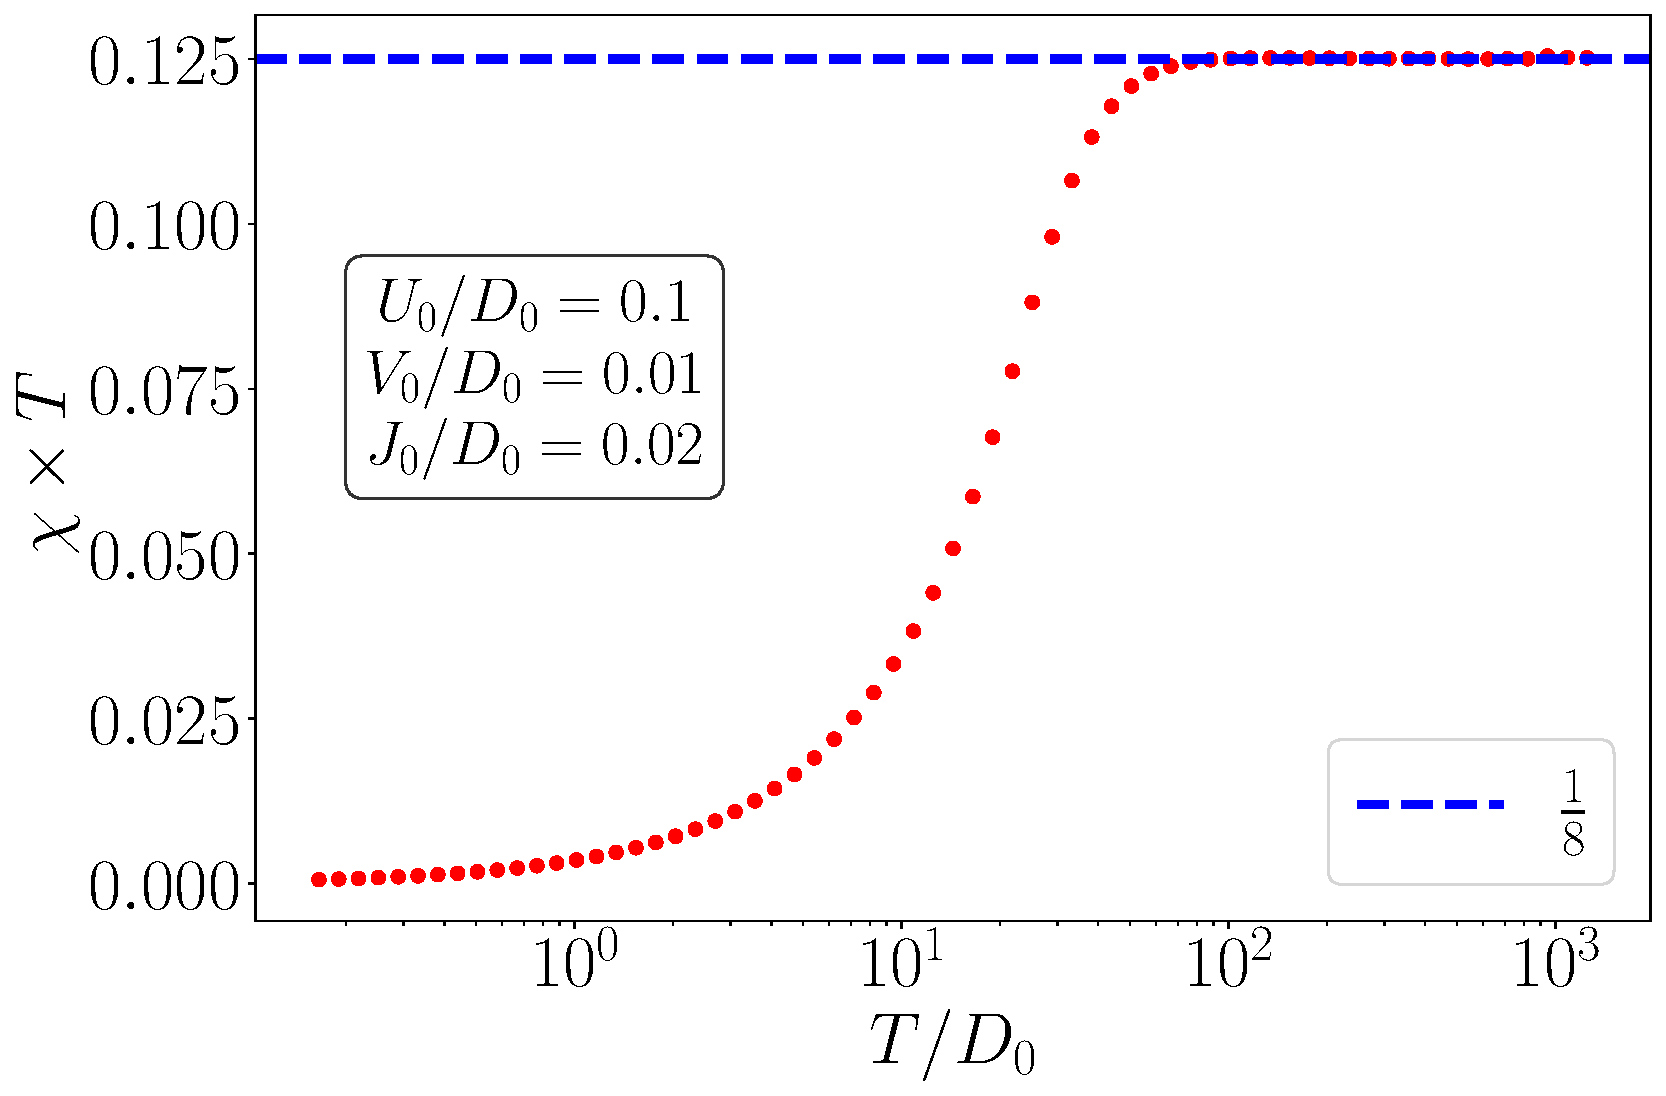
\includegraphics[width=0.49\textwidth]{../figures/chiT_J=0.020.pdf}
	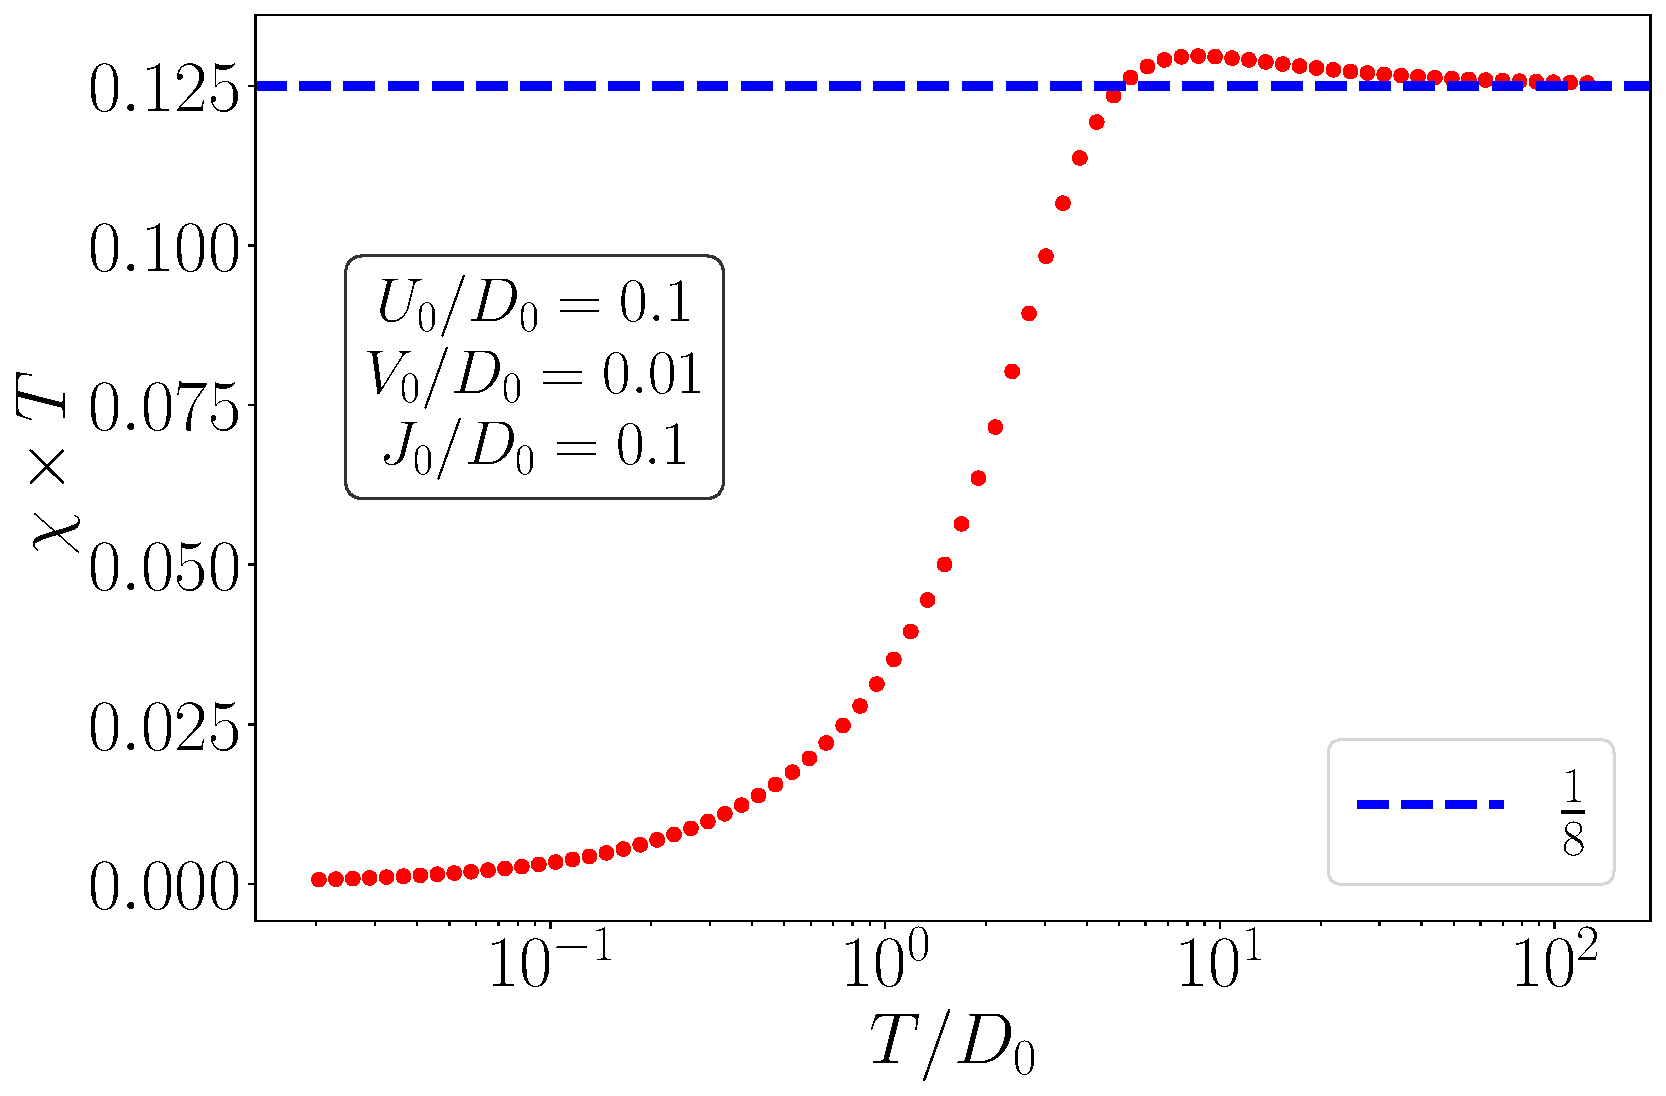
\includegraphics[width=0.49\textwidth]{../figures/chiT_J=0.100.pdf}
	\caption{Spin susceptibility of the impurity times temperature, for two sets of bare parameters, in \(U>0\). At low temperatures, it becomes linear because \(\chi\) itself becomes constant (screening), while at high temperatures, \(\chi\times T\) becomes constant because of the paramagnetic \(\sim 1/T\) form of \(\chi\). For the right panel with a larger value of the spin-exchange coupling, the \(\chi\) tries to go towards the local moment value of \(1/4\) but eventually drops back to the free orbital value of \(1/8\).}
	\label{chi}
\end{figure}

\subsection{Charge susceptibility}
We can similarly define the charge susceptibility as
\begin{equation}\begin{aligned}
	\label{zero_chi_charge}
	\chi(\beta) = \beta \left(\left<\left(C_d^z\right)^2\right> - \left<C_d^z\right>^2\right) = \lim_{B_c \to 0}\frac{1}{\beta}\left[\frac{1}{Z(B_c)} \frac{\partial^2{Z(B_c)}}{\partial{B_c^2}}-\frac{1}{Z(B_c)^2} \left(\frac{\partial{Z(B_c)}}{\partial{B_c}}\right)^2\right]
\end{aligned}\end{equation}
where \(B_c\) is now a field that couples to the impurity charge-isospin:
\begin{equation}\begin{aligned}
	\label{charge_field}
	\mathcal{H}^\prime(B_c) = \mathcal{H} + B_c C_d^z
\end{aligned}\end{equation}
The charge susceptibility for \(U<0\) is shown in fig.~\ref{chi_charge}.
\begin{figure}[htpb]
	\centering
	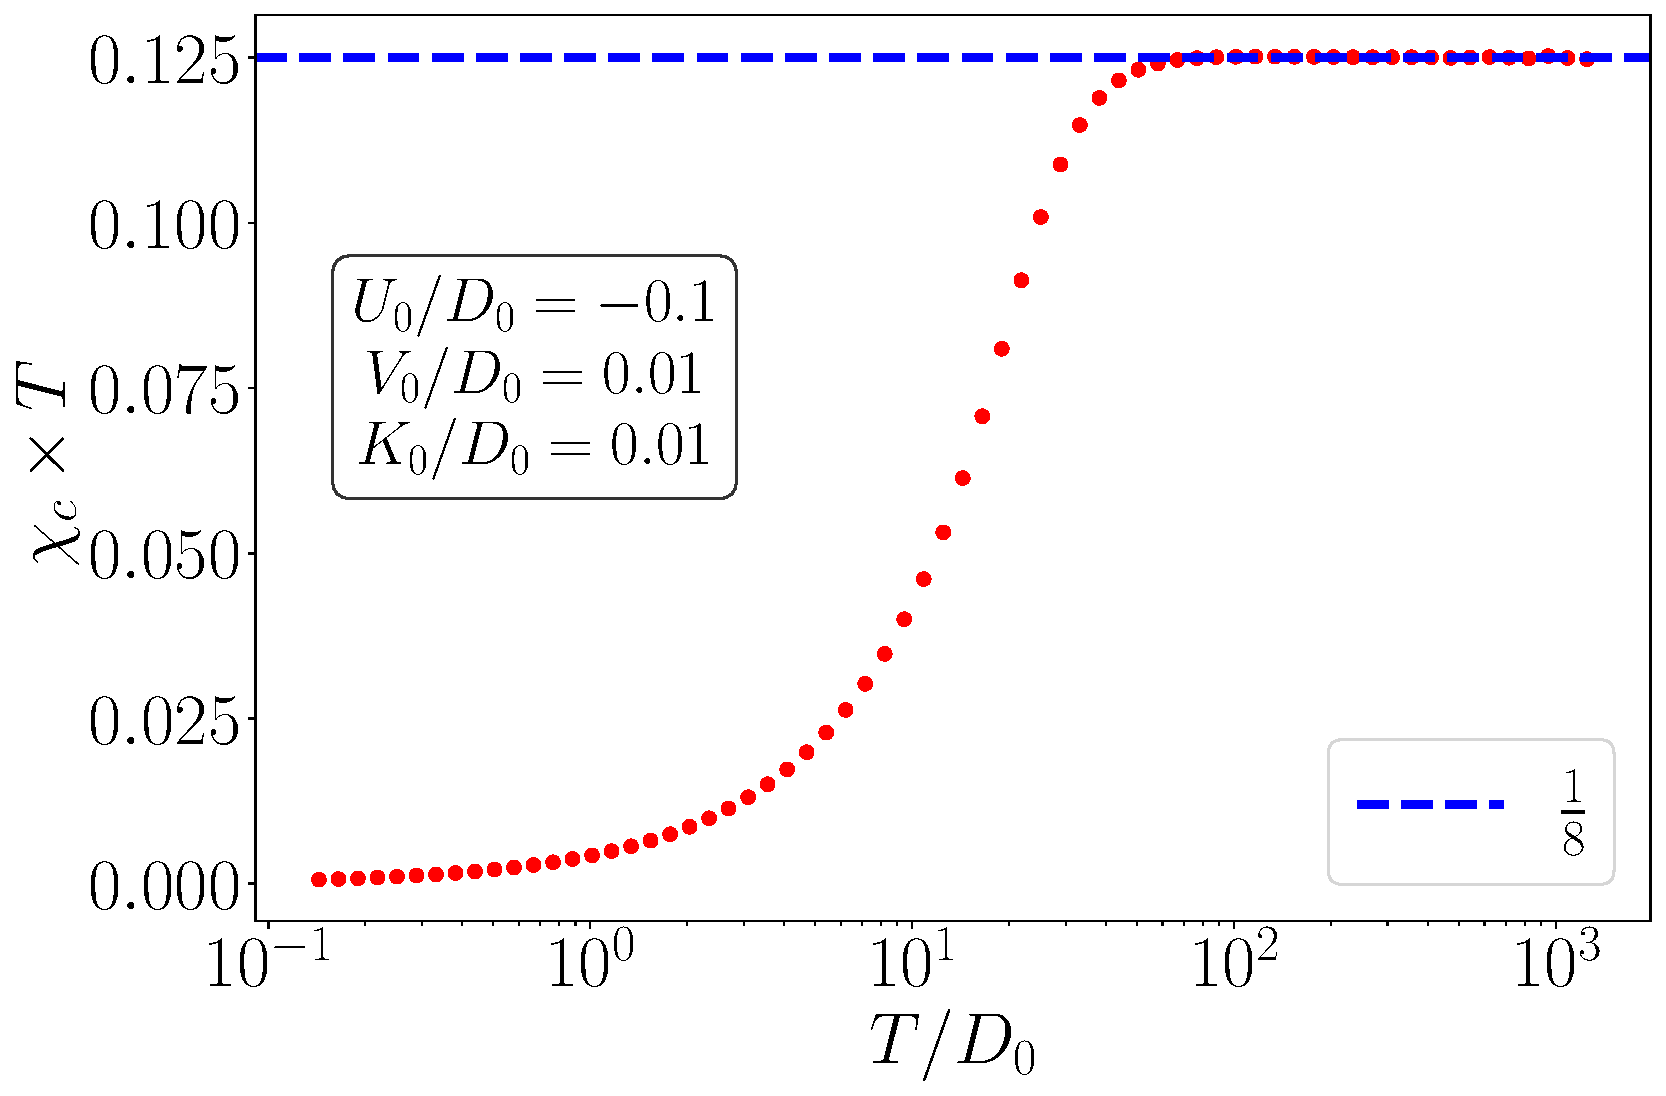
\includegraphics[width=0.49\textwidth]{../figures/chi_chargeT_K=0.010.pdf}
	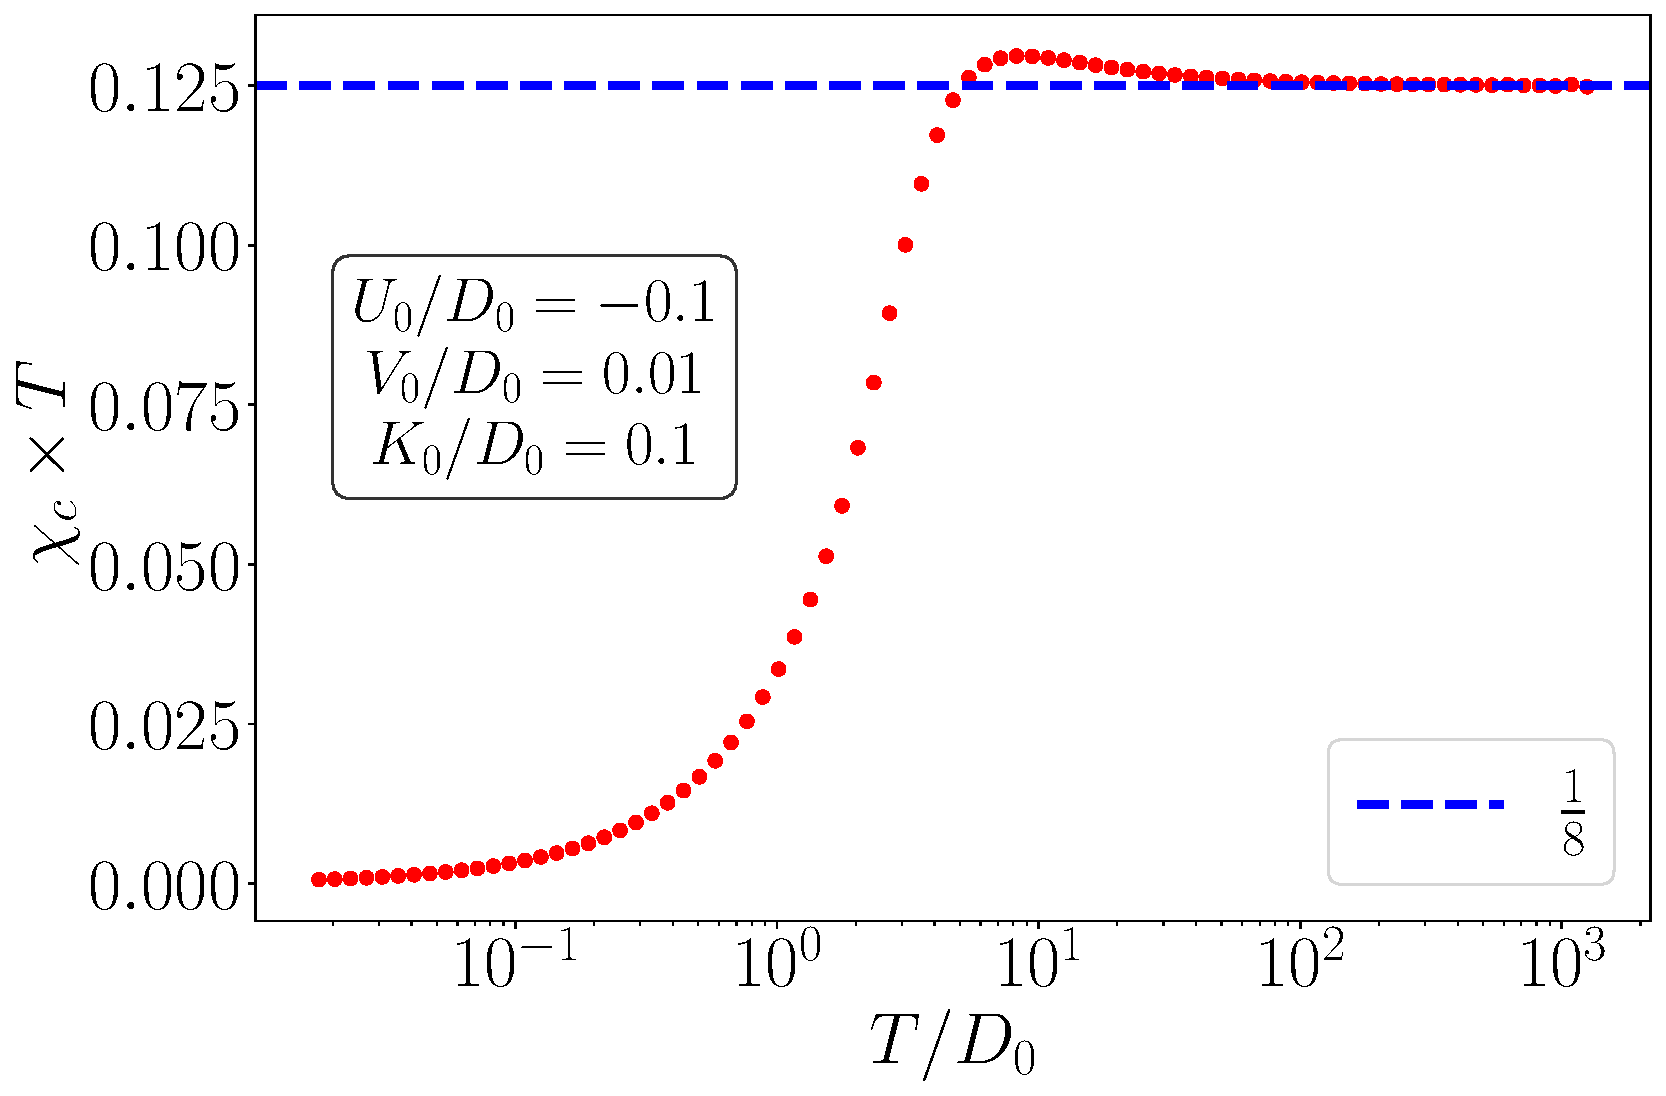
\includegraphics[width=0.49\textwidth]{../figures/chi_chargeT_K=0.100.pdf}
	\caption{Charge susceptibility for the impurity at \(U<0\), for two sets of bare parameters. The physics is very similar to that of the spin susceptibility in \(U>0\).}
	\label{chi_charge}
\end{figure}

It is interesting to look at the behaviour of the charge susceptibility in the positive \(U\) regime, fig.~\ref{chi_charge_posU}. It  is seen that for \(J_0<V_0\), the charge susceptibility is very similar to the spin susceptibility, with a reduced saturation value. This is because, for that range of bare values, the ground state consists of a comparable mixture of the spin and charge states (see fig.~\ref{cs_cc}). This means that the magnetic field term in eq.~\eqref{charge_field} can couple to the charge component of the ground state, and give a non-zero charge susceptibility at zero temperature. On the other hand, for \(J_0 > V_0\), we see that \(\chi_c\) vanishes at low temperatures. This can again be understood from the ground state. For that range of bare values, the ground state can be approximated by purely the singlet, because the charge fraction \(c_-^c\) becomes very small. This means that the field \(B_c \) has nothing to couple with. Alternatively, it can be said that since the ground state has only terms with \(\hat n_d=1\), no number fluctuation is possible, and the impurity isospin is not susceptible at all to charge polarisation.
\begin{figure}[htpb]
	\centering
	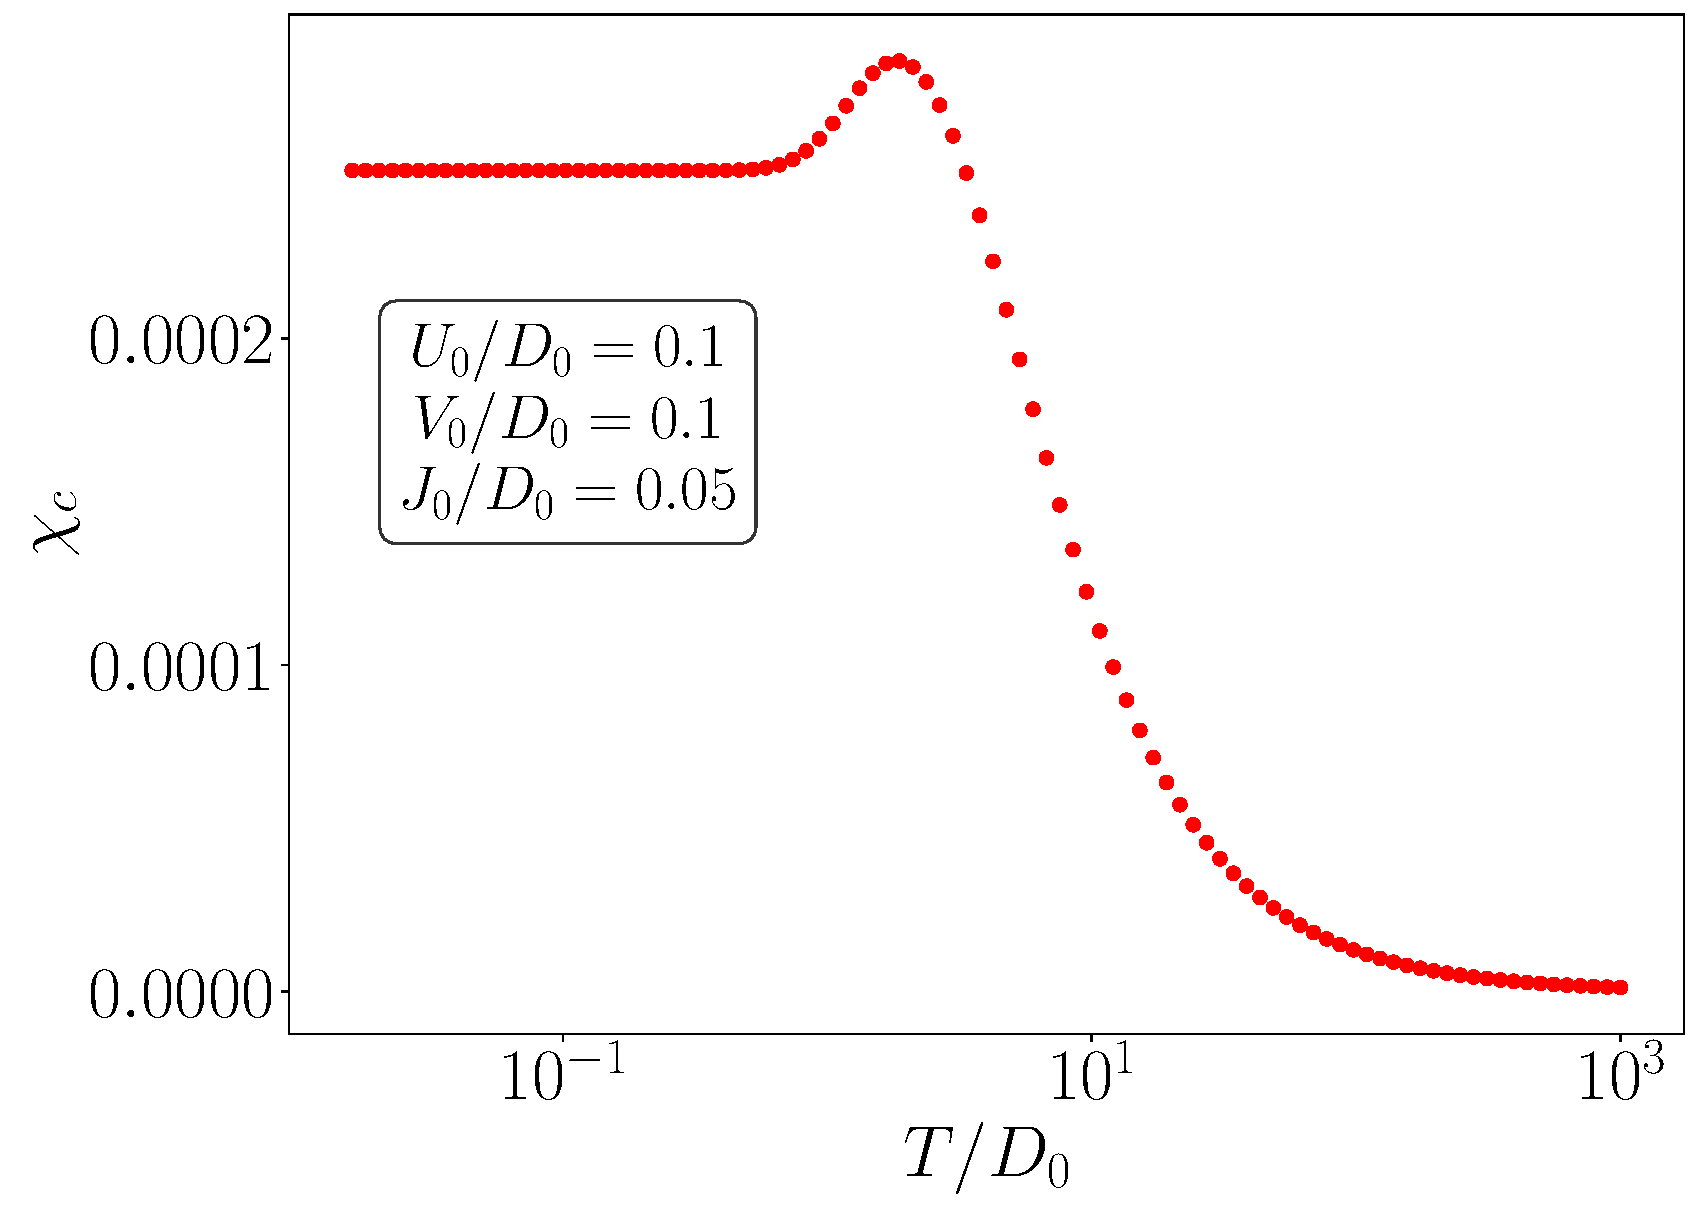
\includegraphics[width=0.48\textwidth]{../figures/chiC_posU_J=small.pdf}
	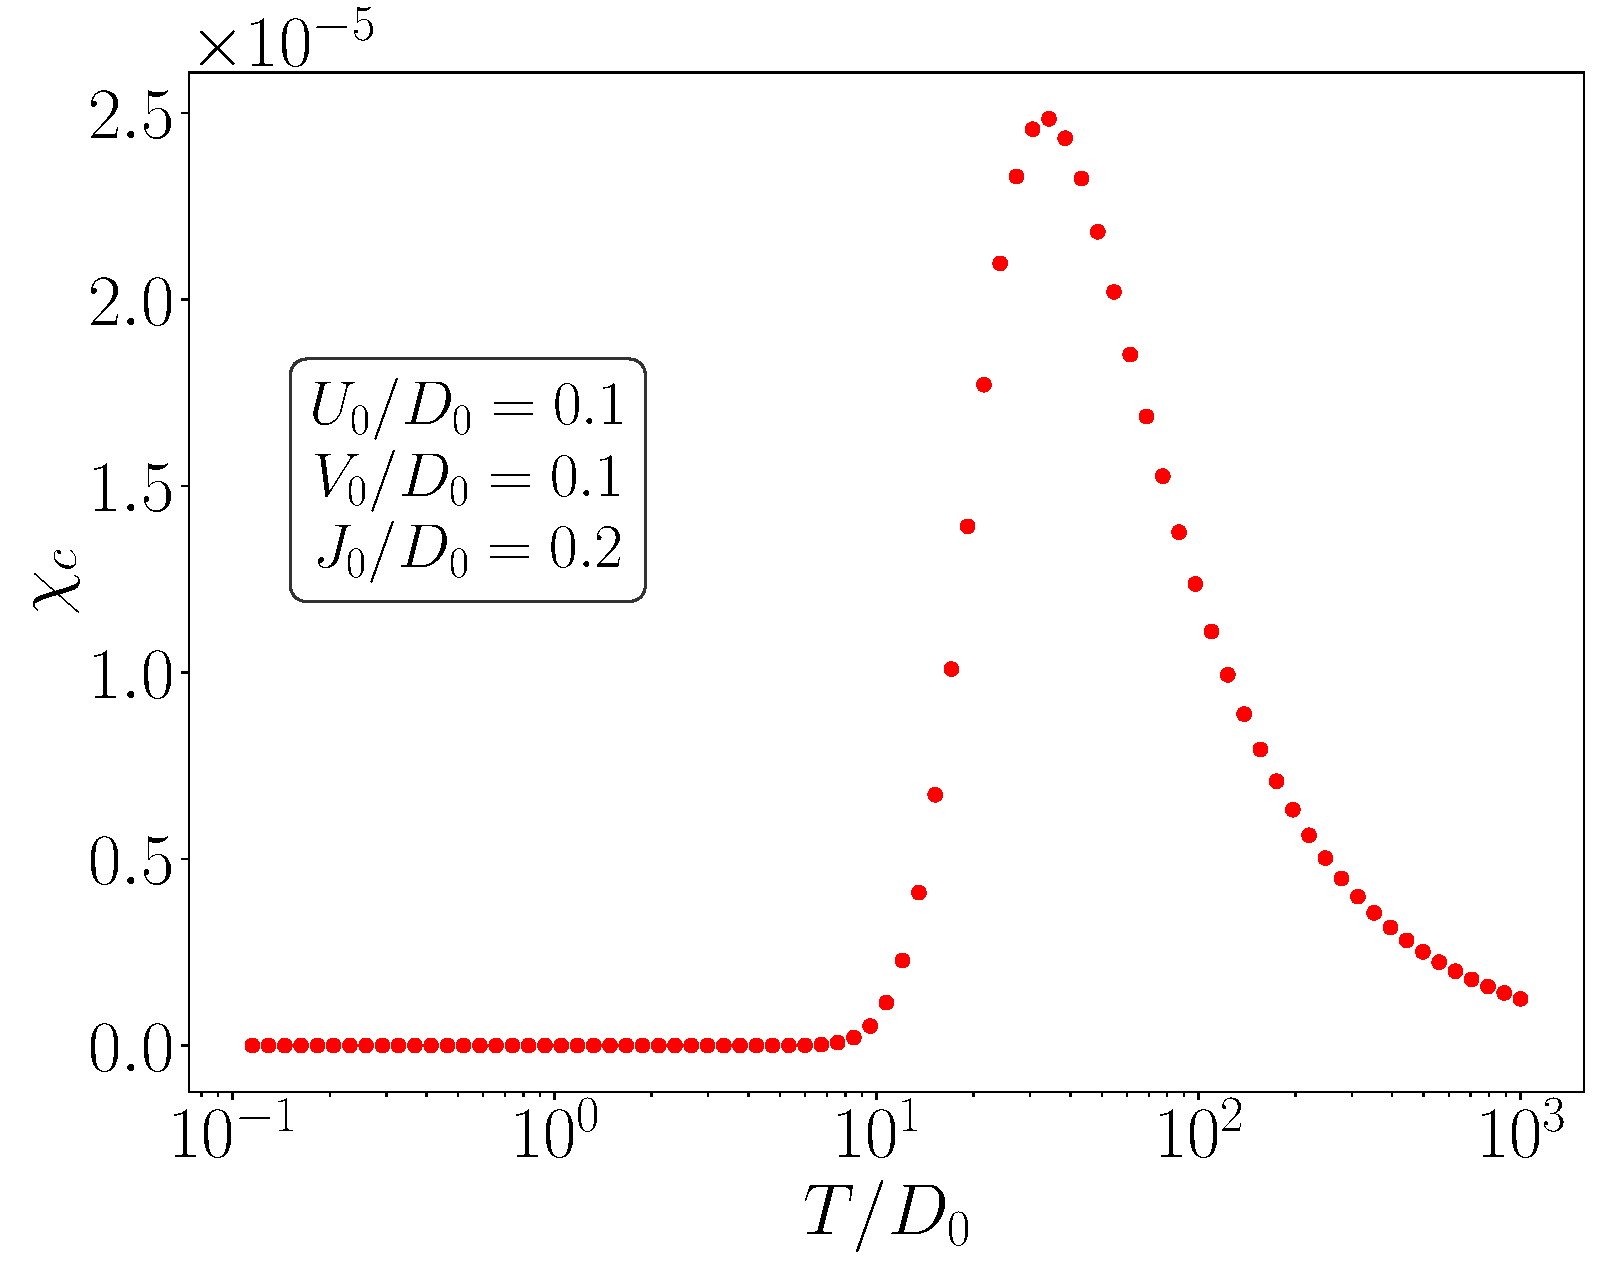
\includegraphics[width=0.48\textwidth]{../figures/chiC_posU_J=large.pdf}
	\caption{Charge susceptibility of the impurity in the positive \(U\) regime, for two values of \(J_0\). The smaller bare value leads to a spin+charge mixed ground state, and hence a non-zero \(\chi_c\) at zero temperature. The larger \(J_0\), however, leads to a purely spin ground state without any number fluctuation, and this gives vanishing \(\chi_c\) at zero temperature.}
	\label{chi_charge_posU}
\end{figure}

From eq.~\eqref{gstate_kondo}, we know that in the thermodynamic limit, the ground state of \(U>0\) regime reduces to a screened local moment. That then implies that the charge susceptibility vanishes at low temperatures, owing to lack of any charge content in the ground state in the large bandwidth limit.
\begin{equation}\begin{aligned}
	\lim_{D_0 \to \infty}\chi_c(U>0, T \to 0) = 0
\end{aligned}\end{equation}

\section{Specific heat}
The specific heat is calculated by diagonalizing the fixed point Hamiltonian, numerically. The obtained spectrum is denoted by \(\left\{ \mathcal{E}_i \right\} \). The total average energy of the impurity+cloud at temperature \(T\) is then
\begin{equation}\begin{aligned}
	\left<\mathcal{E} \right> = \frac{1}{Z}\sum_{i} \mathcal{E}_i e^{-\beta \mathcal{E}_i}
\end{aligned}\end{equation}
where \(Z = \sum_{i} e^{-\beta E_i}\) is the partition function. The specific heat of this system is thus
\begin{equation}\begin{aligned}
	C_V &= \frac{\partial{\left<\mathcal{E} \right>}}{\partial{T}} \\
	    &= -\frac{1}{k_B T^2} \frac{\partial{\left<\mathcal{E} \right>}}{\partial{\beta}} \\
	    &= \frac{1}{k_B T^2}\left[\frac{1}{Z}\sum_i \mathcal{E}_i^2 e^{-\beta \mathcal{E}_i} - \left(\frac{1}{Z}\sum_i \mathcal{E}_i e^{-\beta \mathcal{E}_i}\right)^2 \right] 
\end{aligned}\end{equation}
In the absence of impurity, the eigenvalues of the Hamiltonian are \(\left\{\mathcal{E}_i^0\right\}\) with a partition function \(Z^0 = \sum_{i} e^{-\beta E_i^0}\), so the bath specific heat is
\begin{equation}\begin{aligned}
	C_V^0 &= \frac{1}{k_B T^2}\left[\frac{1}{Z_0}\sum_i \mathcal{E}_i^2 e^{-\beta \mathcal{E}_i^0} - \left(\frac{1}{Z_0}\sum_i \mathcal{E}_i^0 e^{-\beta \mathcal{E}_i^0}\right)^2 \right] 
\end{aligned}\end{equation}
The impurity specific heat is the difference.
\begin{equation}\begin{aligned}
	C_V^\text{imp} = C_V - C_V^0
\end{aligned}\end{equation}
These values were calculated numerically and plotted against temperature in fig.~\ref{cv}.
\begin{figure}[htpb]
	\centering
	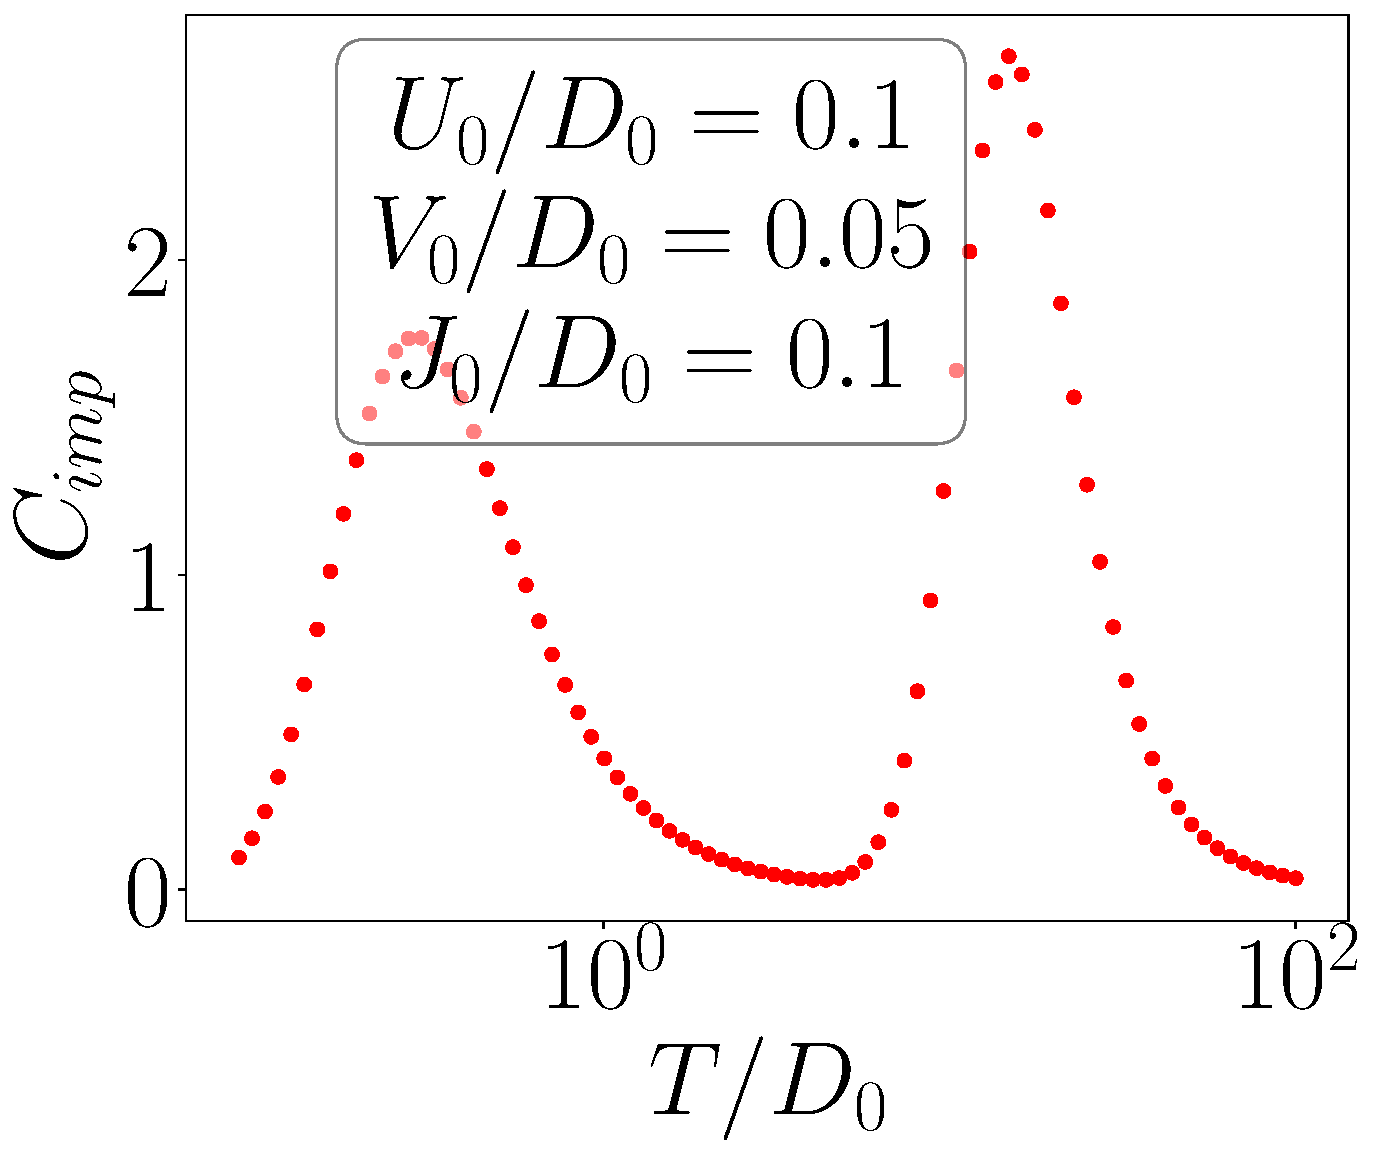
\includegraphics[width=0.6\textwidth]{../figures/Cv.pdf}
	\caption{Impurity specific heat}
	\label{cv}
\end{figure}

\section{Renormalization of impurity spectral function}
In this section we will obtain the impurity spectral function, which is defined in terms of the impurity Green's function as
\begin{equation}\begin{aligned}
	\mathcal{A(\omega)} = -\frac{1}{\pi}\text{ Im }\left[G_{dd}^\sigma\left( \omega \right) \right] 
\end{aligned}\end{equation}
The zero temperature retarded Green's function for the impurity, in the frequency domain, can be written as (see Appendix.~\ref{appx-spectral-func})
\begin{equation}\begin{aligned}
	\mathcal{A(\omega)} = \frac{1}{d_0}\sum_{n,0}\left[||\bra{0}\mathcal{O}_{\sigma}\ket{n}||^2\delta\left(\omega + E_0 - E_n\right) + ||\bra{n}\mathcal{O}_{\sigma}\ket{0}||^2\delta\left(\omega - E_0 + E_n\right)\right]
\end{aligned}\end{equation}
where \(\mathcal{O}_\sigma = c_{d\sigma} + S_d^- c_{0\overline\sigma} + S_d^z c_{0\sigma}\) is the excitation whose spectral function we are interested in. The excitations defined in \(\mathcal{O}\) incorporates both single-particle excitations brought about by the hybridisation as well as two-particle spin excitations brought about by the spin-exchange term
Since this is in terms of the exact eigenstates, it is a discrete sum of delta-functions. In practice, we get a continuous distribution. To compare with experiment, we need to convert the discrete sum into a continuous function. Following \cite{bullaNRGreview}, we replace the delta-functions at \(\pm x_n \equiv \pm(E_n - E_0)\) by normalized Gaussian functions
\begin{equation}\begin{aligned}
	\delta(\omega \pm x_n) \to \frac{1}{\eta_n\sqrt \pi}e^{-\left(\frac{\omega \pm x_n}{\eta_n}\right)^2}
\end{aligned}\end{equation}
The parameter \(\eta_n\) determines the height and width of the Gaussian, and is chosen such that the higher energy poles are broader than the lower energy ones:
\begin{equation}\begin{aligned}
	\eta_n = 4\Delta + \frac{1}{2}|x_n| 
\end{aligned}\end{equation}
\(\Delta = \pi \rho(0)V^2\) is the relevant energy scale for the non-interacting \((U=0)\) problem, \(\rho(0)\) being the density of states of the conduction bath at the Fermi energy. As a result, the function that we will numerically compute and plot is
\begin{equation}\begin{aligned}
	\mathcal{A(\omega)} &= \sum_{n,0}\frac{1}{d_0 \sqrt \pi \eta_n}\left[||\bra{0}c_{d\sigma}\ket{n}||^2e^{-\left(\frac{\omega - x_n}{\eta_n}\right)^2} + ||\bra{n}c_{d\sigma}\ket{0}||^2e^{-\left(\frac{\omega + x_n}{\eta_n}\right)^2}\right]
\end{aligned}\end{equation}
From the results of Langreth \cite{langreth1966}, we know that the spectral function at zero frequency is fixed by the occupancy of the impurity. Since we are in the particle-hole symmetric regime, this occupancy is fixed at 1, and hence so is the spectral function height at \(\omega = 0\). This result has been used to fix the spectral function height at the center during the computations. The fixed-point Hamiltonian \(H^*\) is diagonalized numerically to obtain \(\left\{E_n, \ket{n}\right\}\), for various values of the couplings. The intention here is to get an idea of how the spectral function morphs under the RG. Doing an actual reverse RG (described in \ref{rev_rg}) would require us to diagonalize a huge Hamiltonian. We take the simpler route of tuning the \(U\) from zero to soem large value. This should mimic the journey from the IR theory \((U=0)\) to the UV theory \((U \gg 0)\).

The spectral function is plotted for three sets of values in fig.~\ref{spec_func}. For low values of \(U\), the profile is that of a single peak at zero frequency. This is expected because at the low energy effective theory, the high energy Hubbard side bands have been integrated out. As \(U\) increases, shoulder-like structures appear on either side of the peak, which finally, at larger \(U\), develop into two side-peaks. This is the microscopic theory, where high energy features are also relevant.
\begin{center}
	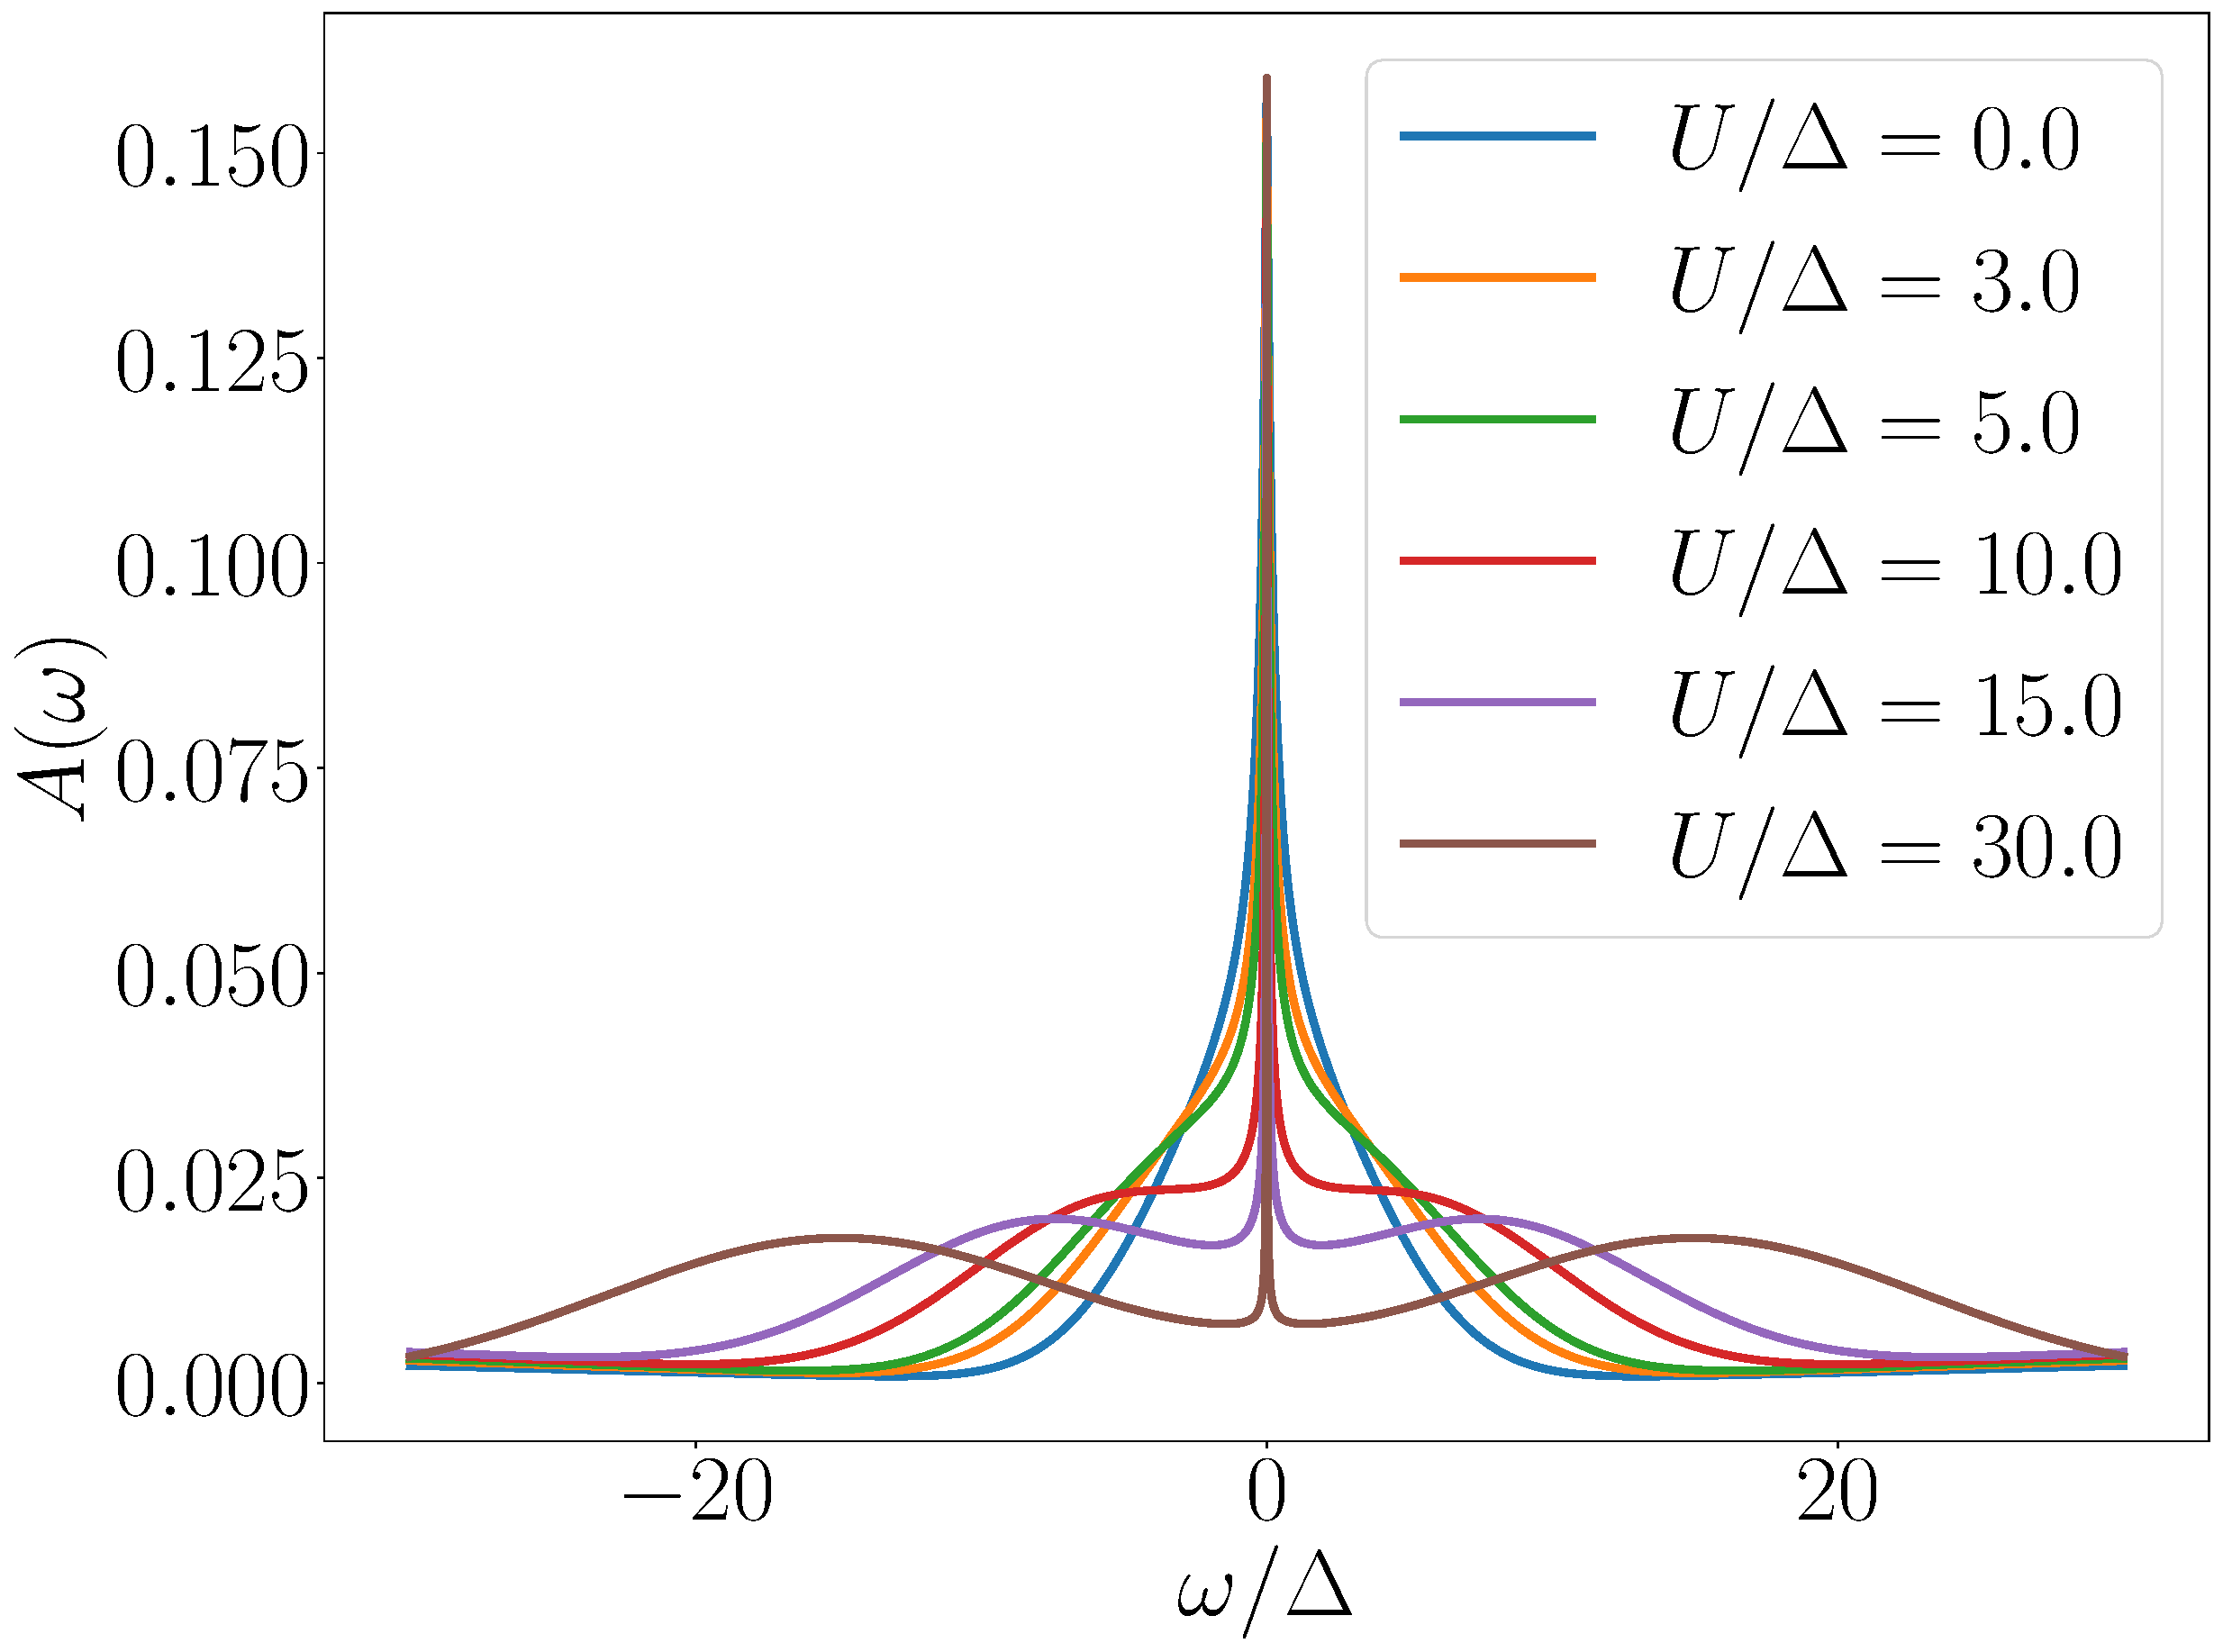
\includegraphics[width=0.8\textwidth]{../figures/gen_siam_spec_func.pdf}
	\captionof{figure}{Impurity spectral function for multiple values of \(U\). The increase in value of \(U\) is accompanied by the appearance of the side-peaks.}
	\label{spec_func}
\end{center}
The physics of the three peaks can now be looked into. Since the central peak is at zero energy, it has to do with excitations that do not cost any energy. There are two such excitations: excitations within the spin sector and within the charge sector.
\begin{equation}\begin{aligned}
	\ket{\uparrow} \mathrel{\mathlarger{\mathlarger{\mathop{\rightleftarrows}}^{J S_d^-}_{JS_d^+}}}\ket{\downarrow}, &&&&\ket{\Uparrow} \mathrel{\mathlarger{\mathlarger{\mathop{\rightleftarrows}}^{K C_d^-}_{K C_d^+}}}\ket{\Downarrow}\\
\end{aligned}\end{equation}
The thick arrow \(\Uparrow\) represents the charge isospin. At particle-hole symmetry, both the spin configurations has energy of \(\epsilon_d\), while the charge configurations have energy of \(2\epsilon_d + U=0\) and 0. Hence, no energy is required for these excitations, which is why see a macroscopic number of cloud electrons resonating with the impurity at the Fermi surface. Also note that if \(\hat S_i\) and \(\hat C_j\) are two operators of the spin and charge sector (\(i,j \in \left\{ x,y,z \right\} \)), then
\begin{equation}\begin{aligned}
	\hat S_i \hat C_j = \hat C_j \hat S_i = 0
\end{aligned}\end{equation}
We can see this by applying that operator on a basis state. Since the set of four states 
\begin{equation}\begin{aligned}
	\ket{\hat S_i = \pm \frac{1}{2}, \hat C_j = 0}, \ket{\hat S_i = 0, \hat C_j = \pm\frac{1}{2}}
\end{aligned}\end{equation}
are all independent, they form a basis. If we apply the operator on these states:
\begin{equation}\begin{aligned}
	\hat S_i \hat C_j \ket{\hat S_i} &= 0, &&&&\hat C_j \hat S_i \ket{S_i} = S_i \hat C_j \ket{S_i} = 0\\
	\hat C_j \hat S_i \ket{C_j} &= 0, &&&&\hat S_i \hat C_j \ket{\hat C_j} = C_j \hat S_i \ket{\hat C_j} = 0 \\
\end{aligned}\end{equation}
This shows that each operator acts only on its own subspace. \(S_i\) does not act on the charge sector, and vice-versa. There is no single-particle excitation here.

The physics of the side-peaks is that of single number fluctuations on the impurity. These are brought about by the term \(Vc^\dagger_{0\sigma}c_{d\sigma} + \text{h.c.}\).
\begin{equation}\begin{aligned}
	\left( \epsilon_d  \right) \ket{\sigma} & \mathrel{\mathlarger{\mathlarger{\mathop{\rightleftarrows}}^{V c^\dagger_{d\overline\sigma}/V c_{d\sigma}}_{V c_{d\overline\sigma}/V c^\dagger_{d\sigma}}}} &\ket{n_d=2,0} \left( 0 \right) \\
\end{aligned}\end{equation}
These transitions involve energy transfer of the order of \(\epsilon_d\). This is why, at very small \(U\), they remain absorbed inside the central peak. These transitions do not involve any spin or charge-flip, rather they take the impurity between the spin and charge sectors.

\section{Effective Hamiltonian for excitations of the Kondo cloud}
To find an effective Hamiltonian for the excitations of the Kondo cloud, we will integrate out the impurity part of the wavefunction. The Schrodinger equation for the \(J > K\) ground state is
\begin{equation}\begin{aligned}
	E_g &\left[c_-^s \left(\ket{\uparrow, \downarrow} - \ket{\downarrow, \uparrow}\right) + c^c_- \left(\ket{\uparrow\downarrow, 0} + \ket{0, \uparrow\downarrow}\right)\right] \\
	    &= \mathcal{H} \left[c_-^s \left(\ket{\uparrow, \downarrow} - \ket{\downarrow, \uparrow}\right) + c^c_- \left(\ket{\uparrow\downarrow, 0} + \ket{0, \uparrow\downarrow}\right)\right]\\
	    &= \mathcal{H}_0^* \left[c_-^s \left(\ket{\uparrow, \downarrow} - \ket{\downarrow, \uparrow}\right) + c^c_- \left(\ket{\uparrow\downarrow, 0} + \ket{0, \uparrow\downarrow}\right)\right]\\
	    &+V\sum_{\beta}\left[c^\dagger_{2\beta}c_{1\beta} - c_{2\beta}c^\dagger_{1\beta}\right]\left[c_-^s \left(\ket{\uparrow, \downarrow} - \ket{\downarrow, \uparrow}\right) + c^c_- \left(\ket{\uparrow\downarrow, 0} + \ket{0, \uparrow\downarrow}\right)\right]\\
	    &+ J \vec{S_d}\cdot\vec{s}\left[c_-^s \left(\ket{\uparrow, \downarrow} - \ket{\downarrow, \uparrow}\right) + c^c_- \left(\ket{\uparrow\downarrow, 0} + \ket{0, \uparrow\downarrow}\right)\right]\\
	    &+ K \vec{C_d}\cdot\vec{c}\left[c_-^s \left(\ket{\uparrow, \downarrow} - \ket{\downarrow, \uparrow}\right) + c^c_- \left(\ket{\uparrow\downarrow, 0} + \ket{0, \uparrow\downarrow}\right)\right]
\end{aligned}\end{equation}
The last two lines gives
\begin{equation}\begin{aligned}
\frac{1}{2}Jc_-^s \left[s^z \left(\ket{\uparrow, \downarrow} + \ket{\downarrow, \uparrow}\right) +  s^+ \ket{\downarrow, \downarrow} - s^-\ket{\uparrow, \uparrow}\right] + \frac{1}{2}Kc^c_- \left[c^z\left(\ket{\uparrow\downarrow, 0} - \ket{0, \uparrow\downarrow}\right) + c^+\ket{0, 0} \right.\\
+ \left.c^-\ket{2, 2}\right]
\end{aligned}\end{equation}
The second line gives
\begin{equation}\begin{aligned}
	V c^\dagger_{2\uparrow}\left[c_-^s \left(\ket{0, \downarrow}\right) + c^c_- \left(\ket{\downarrow, 0}\right)\right] + V c^\dagger_{2 \downarrow}\left[c_-^s \left(- \ket{0, \uparrow}\right) + c^c_- \left(\ket{\uparrow, 0}\right)\right] \\
	- Vc_{2 \uparrow}\left[c_-^s \left(- \ket{ \uparrow\downarrow, \uparrow}\right) + c^c_- \left(\ket{\uparrow, \uparrow\downarrow}\right)\right] - V c_{2 \downarrow}\left[c_-^s \left(-\ket{ \uparrow\downarrow, \downarrow}\right) + c^c_- \left(\ket{ \downarrow, \uparrow\downarrow}\right)\right]
\end{aligned}\end{equation}
We will now write down four equations by comparing the coefficients of \(\ket{ \uparrow}, \ket{ \downarrow}, \ket{0}\) and \(\ket{2}\) of the impurity sector:
\begin{equation}\begin{aligned}
	\left( E_g - H_0^* \right) c_-^s \ket{\downarrow} &= V c^c_- \left( c^\dagger_{2 \downarrow}\ket{0} - c_{2 \uparrow}\ket{2} \right) + \frac{1}{2}J c^s_-\left( s^z\ket{ \downarrow} - s^-\ket{\uparrow} \right) && \left[\text{eq. from }\ket{\uparrow}\right] \\
	\left( -E_g + H_0^* \right) c_-^s \ket{\uparrow} &= V c^c_- \left( c^\dagger_{2 \uparrow}\ket{0} - c^\dagger_{2 \downarrow}\ket{2} \right) + \frac{1}{2}J c^s_-\left( s^z\ket{\uparrow} + s^+\ket{ \downarrow} \right)&& \left[\text{eq. from }\ket{\downarrow}\right] \\
	\left( E_g - H_0^* \right) c_-^c \ket{2} &= V c^s_- \left( c^\dagger_{2 \uparrow}\ket{ \downarrow} - c^\dagger_{2 \downarrow}\ket{ \uparrow} \right) + \frac{1}{2}K c^c_-\left( -c^z\ket{2} + c^+\ket{0} \right) && \left[\text{eq. from }\ket{0}\right] \\
	\left( E_g - H_0^* \right) c_-^c \ket{0} &= V c^s_- \left( c_{2 \uparrow}\ket{ \uparrow} + c_{2 \downarrow}\ket{ \downarrow} \right) + \frac{1}{2}K c^c_-\left( c^z\ket{0} + c^-\ket{2} \right) && \left[\text{eq. from }\ket{2}\right]
\end{aligned}\end{equation}
These can be rearranged into
\begin{equation}\begin{aligned}
	\left( E_g - H_0^* - \frac{1}{2}J s^z\right) \ket{\downarrow} &= V \lambda^{-1} \left( c^\dagger_{2 \downarrow}\ket{0} - c_{2 \uparrow}\ket{2} \right) - \frac{1}{2}J s^-\ket{\uparrow} \\
	\left( E_g - H_0^*  + \frac{1}{2}J s^z\right) \ket{\uparrow} &= V \lambda^{-1} \left( c_{2 \downarrow}\ket{2} - c^\dagger_{2 \uparrow}\ket{0}\right) - \frac{1}{2}J s^+\ket{ \downarrow} \\
	\left( E_g - H_0^*  + \frac{1}{2}K c^z\right)  \ket{2} &= V \lambda \left( c^\dagger_{2 \uparrow}\ket{ \downarrow} - c^\dagger_{2 \downarrow}\ket{ \uparrow} \right) + \frac{1}{2}K c^+\ket{0}  \\
	\left( E_g - H_0^* - \frac{1}{2}K c^z\right)  \ket{0} &= V \lambda \left( c_{2 \uparrow}\ket{ \uparrow} + c_{2 \downarrow}\ket{ \downarrow} \right) + \frac{1}{2}K c^-\ket{2} 
\end{aligned}\end{equation}
where \(\lambda = \frac{c^s_-}{c^c_-}\). We want to find the effective Hamiltonian in the subspace of \(\ket{\downarrow}\). We first eliminate the charge sector from these equations:
\begin{equation}\begin{aligned}
	\ket{0} =& V\lambda\left[\frac{1}{A^K_-}c_{2 \uparrow} + \frac{K}{2}\frac{1}{A^K_-}c^- \frac{1}{A^K_+ - \left( \frac{K}{2} \right) ^2 c^+ \frac{1}{A^K_-}c^-}\left(\frac{K}{2}c^+ \frac{1}{A^K_-}c_{2 \uparrow}- c^\dagger_{2 \downarrow}\right)\right]\ket{ \uparrow} \\
		 &+V\lambda\left[\frac{1}{A^K_-}c_{2 \downarrow} + \frac{K}{2}\frac{1}{A^K_-}c^- \frac{1}{A^K_+ - \left( \frac{K}{2} \right) ^2 c^+ \frac{1}{A^K_-}c^-}\left(c^\dagger_{2 \uparrow} + \frac{K}{2}c^+ \frac{1}{A^K_-}c_{2 \downarrow}\right)\right]\ket{ \downarrow}\\
	\ket{2} &= \frac{V\lambda}{A^K_+ - \left( \frac{K}{2} \right) ^2 c^+ \frac{1}{A^K_-}c^-}\left[\left(c^\dagger_{2 \uparrow} + \frac{K}{2}c^+ \frac{1}{A^K_-}c_{2 \downarrow}\right)\ket{ \downarrow} + \left(\frac{K}{2}c^+ \frac{1}{A^K_-}c_{2 \uparrow}- c^\dagger_{2 \downarrow}\right)\ket{ \uparrow}\right] 
\end{aligned}\end{equation}
where
\begin{equation}\begin{aligned}
	A^K_\pm = E_g - H_0^* \pm \frac{1}{2}Kc^z
\end{aligned}\end{equation}
For ease of labeling, we will think of these equations as
\begin{equation}\begin{aligned}
	\ket{0} = a_0^\uparrow \ket{ \uparrow} + a_0^\downarrow\ket{ \downarrow}, \ket{2} = a_2^\uparrow \ket{ \uparrow} + a_2^\downarrow\ket{ \downarrow}
\end{aligned}\end{equation}
The remaining two equations can then be written as
\begin{equation}\begin{aligned}
	A^J_-\ket{ \downarrow} &= \frac{V}{\lambda}\left[ c^\dagger_{2 \downarrow}\left(a_0^\uparrow \ket{ \uparrow} + a_0^\downarrow\ket{ \downarrow}\right) - c_{2 \uparrow}\left(a_2^\uparrow \ket{ \uparrow} + a_2^\downarrow\ket{ \downarrow}\right) \right] - \frac{J}{2}s^- \ket{ \uparrow}\\
	A^J_+\ket{\uparrow} &= \frac{V}{\lambda}\left[ c_{2 \downarrow}\left(a_2^\uparrow \ket{ \uparrow} + a_2^\downarrow\ket{ \downarrow}\right) - c^\dagger_{2 \uparrow}\left(a_0^\uparrow \ket{ \uparrow} + a_0^\downarrow\ket{ \downarrow}\right) \right]  - \frac{J}{2}s^+ \ket{ \downarrow}\\
\end{aligned}\end{equation}
where 
\begin{equation}\begin{aligned}
	A^J_\pm = E_g - H_0^* \pm \frac{1}{2}Js^z
\end{aligned}\end{equation}
Eliminating \(\ket{\downarrow}\) and solving for \(\ket{\uparrow}\) gives
\begin{equation}\begin{aligned}
	A^J_+ \ket{\uparrow} =&  \frac{V}{\lambda}\left( c_{2 \downarrow}a_2^\uparrow - c^\dagger_{2 \uparrow}a_0^\uparrow \right) \ket{\uparrow} + \left( \frac{V}{\lambda}c_{2 \downarrow}a_2^\downarrow - \frac{V}{\lambda}c^\dagger_{2 \uparrow}a_0^\downarrow - \frac{J}{2}s^+ \right) \ket{\downarrow}\\
			     =& \frac{V}{\lambda}\left( c_{2 \downarrow}a_2^\uparrow - c^\dagger_{2 \uparrow}a_0^\uparrow \right) \ket{\uparrow} \\
			     +& \left[ \frac{V}{\lambda}\left(c_{2 \downarrow}a_2^\downarrow - c^\dagger_{2 \uparrow}a_0^\downarrow\right) - \frac{J}{2}s^+ \right] \frac{1}{A^J_- - \frac{V}{\lambda}\left( c^\dagger_{2 \downarrow}a_0^\downarrow - c_{2 \uparrow}a_2^\downarrow \right) }\left[\frac{V}{\lambda}\left( c^\dagger_{2 \downarrow}a_0^\uparrow - c_{2 \uparrow}a_2^\uparrow\right) - \frac{J}{2}s^-\right] \ket{\uparrow}
\end{aligned}\end{equation}
The effective Hamiltonian for the \(\ket{\uparrow}\) state is
\begin{equation}\begin{aligned}
	\label{full_ham}
	H_0^* - \frac{J}{2}s^z + \frac{V}{\lambda}\left(c_{2 \downarrow}a_2^\uparrow - c^\dagger_{2 \uparrow}a_0^\uparrow \right) + \left[ \frac{V}{\lambda}\left(c_{2 \downarrow}a_2^\downarrow - c^\dagger_{2 \uparrow}a_0^\downarrow\right) - \frac{J}{2}s^+ \right] \frac{1}{A^J_- - \frac{V}{\lambda}\left( c^\dagger_{2 \downarrow}a_0^\downarrow - c_{2 \uparrow}a_2^\downarrow \right) }\\
	\times\left[\frac{V}{\lambda}\left( c^\dagger_{2 \downarrow}a_0^\uparrow - c_{2 \uparrow}a_2^\uparrow\right) - \frac{J}{2}s^-\right]
\end{aligned}\end{equation}
To get a clearer picture of this effective Hamiltonian, we will keep up to two-particle interactions. We first write down the full forms of \(a_{0,2}^\sigma\):
\begin{equation}\begin{aligned}
	a_0^\sigma &= V\lambda\left[\frac{1}{A^K_-}c_{2 \sigma} + \frac{K}{2}\frac{1}{A^K_-}c^- \frac{1}{A^K_+ - \left( \frac{K}{2} \right) ^2 c^+ \frac{1}{A^K_-}c^-}\left(\frac{K}{2}c^+ \frac{1}{A^K_-}c_{2 \sigma}- \sigma c^\dagger_{2 \sigma}\right)\right]\\
	a_2^\sigma &= \frac{V\lambda}{A^K_+ - \left( \frac{K}{2} \right) ^2 c^+ \frac{1}{A^K_-}c^-}\left(-\sigma c^\dagger_{2 -\sigma} + \frac{K}{2}c^+ \frac{1}{A^K_-}c_{2 \sigma}\right)
\end{aligned}\end{equation}
We will first look at the special case of \(K = 0\). There, the above expressions simplify to
\begin{equation}\begin{aligned}
	a_0^\sigma &= V\lambda\frac{1}{A^K_-}c_{2 \sigma} = \frac{V \lambda}{E_g}\left[ 1 + \frac{1}{E_g}\left(H_0^* \right) + \frac{1}{E_g^2}\left(H_0^* \right)^2\right] c_{2\sigma} + \mathcal{O}({H_0^*}^3)\\
	a_2^\sigma &= -\sigma V\lambda\frac{1}{A^K_+}c^\dagger_{2 -\sigma} = -\sigma\frac{V \lambda}{E_g}\left[ 1 + \frac{1}{E_g}\left(H_0^* \right) + \frac{1}{E_g^2}\left(H_0^* \right)^2\right] c^\dagger_{2 -\sigma} + \mathcal{O}({H_0^*}^3)\\
\end{aligned}\end{equation}
We will make use of the following commutators:
\begin{equation}\begin{aligned}
	&\left[\left(H_0^*\right)^m, c_{2\sigma}\right] = - \sum_k \frac{\epsilon^m_k}{\sqrt{N^*}}c_{k\sigma}, && \left[\left(H_0^*\right)^m, c^\dagger_{2\sigma}\right] = \sum_k \frac{\epsilon_k^m}{\sqrt{N^*}}c^\dagger_{k\sigma}, && m = 1, 2\\
	&\left[\left(H_0^*\right)^m, s^+\right] = \sum_{kk^\prime}\left(\epsilon_k^m - \epsilon_{k^\prime}^m\right)c^\dagger_{k\beta}c_{k^\prime \overline \beta} , &&&& m = 1, 2\\
	&\left[\left(s^z\right)^m, c_{2\sigma}\right] = - \left(\frac{\sigma}{2}\right)^mc_{2\sigma}, && \left[\left(s^z\right)^m, c^\dagger_{2\sigma}\right] = \left(\frac{\sigma}{2}\right)^mc^\dagger_{2\sigma}, && m = 1, 2\\
	&\left[\left(c^z\right)^m, c_{2\sigma}\right] = - \left(\frac{1}{2}\right)^mc_{2\sigma}, && \left[\left(c^z\right)^m, c^\dagger_{2\sigma}\right] = \left(\frac{1}{2}\right)^mc^\dagger_{2\sigma}, && m = 1, 2\\
\end{aligned}\end{equation}
Now we evaluate the various terms in the effective Hamiltonian.
\begin{flalign*}
	{{c_{2 \downarrow}a_2^\uparrow}} &= -\frac{V \lambda}{E_g}c_{2 \downarrow}\left[ 1 + \frac{1}{E_g}\left(H_0^* \right) + \frac{1}{E_g^2}\left(H_0^* \right)^2\right] c^\dagger_{2\downarrow}\\
				     &= -\frac{V \lambda}{E_g}\left[c_{2 \downarrow} + \frac{1}{E_g}\left(H_0^* \right)c_{2 \downarrow} + \sum_k \frac{\epsilon_k}{E_g\sqrt{N^*}}c_{k\downarrow} + \frac{1}{E_g^2}\left(H_0^* \right)^2c_{2 \downarrow} + \sum_k \frac{\epsilon^2_k}{E_g^2\sqrt{N^*}}c_{k\downarrow}\right]c^\dagger_{2\downarrow}\\
				     &= -\frac{V \lambda}{E_g}\left[1 + \frac{H_0^*}{E_g} + \left(\frac{H_0^*}{E_g}\right)^2\right]c_{2 \downarrow}c^\dagger_{2\downarrow} - \frac{V \lambda}{E_g N^*}\sum_{kk^\prime} \left(\frac{\epsilon_k }{E_g}+ \frac{\epsilon_k^2}{E_g^2}\right)c_{k\downarrow}c^\dagger_{k^\prime\downarrow}\\
{{c_{2 \uparrow}a_2^\downarrow }}&= -\frac{V \lambda}{E_g}\left[1 + \frac{H_0^*}{E_g} + \left(\frac{H_0^*}{E_g}\right)^2\right]c_{2 \uparrow}c^\dagger_{2\uparrow} - \frac{V \lambda}{E_g N^*}\sum_{kk^\prime} \left(\frac{\epsilon_k }{E_g}+ \frac{\epsilon_k^2}{E_g^2}\right) c_{k\uparrow}c^\dagger_{k^\prime\uparrow}\\
{{c^\dagger_{2 \uparrow}a_0^\uparrow}} &= c^\dagger_{2 \uparrow} \frac{V \lambda}{E_g}\left[ 1 + \frac{1}{E_g}\left(H_0^* \right) + \frac{1}{E_g^2}\left(H_0^* \right)^2\right] c_{2 \uparrow}\\
					   &= \frac{V \lambda}{E_g}\left[1 + \frac{H_0^*}{E_g} + \left(\frac{H_0^*}{E_g}\right)^2\right]c^\dagger_{2 \uparrow}c_{2\uparrow} - \frac{V \lambda}{E_g N^*}\sum_{kk^\prime} \left(\frac{\epsilon_k }{E_g}+ \frac{\epsilon_k^2}{E_g^2}\right)c^\dagger_{k\uparrow}c_{k^\prime\uparrow}\\
{{c^\dagger_{2 \downarrow}a_0^\downarrow}} &= \frac{V \lambda}{E_g}\left[1 + \frac{H_0^*}{E_g} + \left(\frac{H_0^*}{E_g}\right)^2\right]c^\dagger_{2 \downarrow}c_{2\downarrow} - \frac{V \lambda}{E_g N^*}\sum_{kk^\prime} \left(\frac{\epsilon_k }{E_g}+ \frac{\epsilon_k^2}{E_g^2}\right)c^\dagger_{k\downarrow}c_{k^\prime\downarrow}\\
{{c_{2 \downarrow}a_2^\downarrow }}&= \frac{V \lambda}{E_g}c_{2 \downarrow}\left[ 1 + \frac{1}{E_g}\left(H_0^* \right) + \frac{1}{E_g^2}\left(H_0^* \right)^2\right] c^\dagger_{2\uparrow}\\
				       &=\frac{V \lambda}{E_g}\left[1 + \frac{1}{E_g}\left(H_0^* \right)\right]c_{2 \downarrow}c^\dagger_{2\uparrow} + \frac{V \lambda}{E_g N^*}\sum_{kk^\prime} \left(\frac{\epsilon_k }{E_g}+ \frac{\epsilon_k^2}{E_g^2}\right)c_{k\downarrow}c^\dagger_{k^\prime\uparrow}\\
{{c_{2 \uparrow}a_2^\uparrow}} &=-\frac{V \lambda}{E_g}\left[1 + \frac{1}{E_g}\left(H_0^* \right)\right]c_{2 \uparrow}c^\dagger_{2\downarrow} - \frac{V \lambda}{E_g N^*}\sum_{kk^\prime} \left(\frac{\epsilon_k }{E_g}+ \frac{\epsilon_k^2}{E_g^2}\right)c_{k\uparrow}c^\dagger_{k^\prime\downarrow}\\
{{c^\dagger_{2 \uparrow}a_0^\downarrow }}&= \frac{V \lambda}{E_g}\left[1 + \frac{H_0^*}{E_g}\right]c^\dagger_{2 \uparrow}c_{2\downarrow} - \frac{V \lambda}{E_g N^*}\sum_{kk^\prime} \left(\frac{\epsilon_k }{E_g}+ \frac{\epsilon_k^2}{E_g^2}\right)c^\dagger_{k\uparrow}c_{k^\prime\downarrow}\\
{{c^\dagger_{2 \downarrow}a_0^\uparrow}} &= \frac{V \lambda}{E_g}\left[1 + \frac{H_0^*}{E_g}\right]c^\dagger_{2 \downarrow}c_{2\uparrow} - \frac{V \lambda}{E_g N^*}\sum_{kk^\prime} \left(\frac{\epsilon_k }{E_g}+ \frac{\epsilon_k^2}{E_g^2}\right)c^\dagger_{k\downarrow}c_{k^\prime\uparrow}\\
{{c_{2 \downarrow}a_2^\uparrow - c^\dagger_{2 \uparrow}a_0^\uparrow}} &= -\frac{V \lambda}{E_g}\left[1 + \frac{H_0^*}{E_g} + \left(\frac{H_0^*}{E_g}\right)^2\right]\times 2 + \frac{V \lambda}{E_g N^*}\sum_{kk^\prime} \left(\frac{\epsilon_k }{E_g}+ \frac{\epsilon_k^2}{E_g^2}\right)\left(c^\dagger_{k\uparrow}c_{k^\prime\uparrow} - c_{k\downarrow}c^\dagger_{k^\prime\downarrow}\right)\\
{{c_{2 \downarrow}a_2^\downarrow - c^\dagger_{2 \uparrow}a_0^\downarrow }}&= \frac{V \lambda}{E_g}\left[1 + \frac{1}{E_g}\left(H_0^* \right)\right]c_{2 \downarrow}c^\dagger_{2\uparrow} \times 2 + \frac{V \lambda}{E_g N^*}\sum_{kk^\prime} \left(\frac{\epsilon_k }{E_g}+ \frac{\epsilon_k^2}{E_g^2}\right)\left(c_{k\downarrow}c^\dagger_{k^\prime\uparrow} + c^\dagger_{k\uparrow}c_{k^\prime\downarrow}\right)\\
{{c^\dagger_{2 \downarrow}a_0^\downarrow - c_{2 \uparrow}a_2^\downarrow}} &= \frac{V \lambda}{E_g N^*}\sum_{kk^\prime} \left(\frac{\epsilon_k }{E_g}+ \frac{\epsilon_k^2}{E_g^2}\right)\left(c_{k\uparrow}c^\dagger_{k^\prime\uparrow} - c^\dagger_{k\downarrow}c_{k^\prime\downarrow}\right)\\
	{{c^\dagger_{2 \downarrow}a_0^\uparrow - c_{2 \uparrow}a_2^\uparrow}} &= \frac{V \lambda}{E_g N^*}\sum_{kk^\prime} \left(\frac{\epsilon_k }{E_g}+ \frac{\epsilon_k^2}{E_g^2}\right)\left(c_{k\uparrow}c^\dagger_{k^\prime\downarrow} - c^\dagger_{k\downarrow}c_{k^\prime\uparrow}\right)
\end{flalign*}
In all the expressions, we have dropped terms that have more than 4 operators in product. Also, in the last four equations, we have substituted \(\hat n_{2 \uparrow} - \hat n_{2 \downarrow} = 1\), because this is the effective Hamiltonian for the state with \(s^z = \frac{1}{2}\). We now substitute these expressions into the effective Hamiltonian:
\begin{equation}\begin{aligned}
	&H_0^* - \frac{J}{2}s^z -\frac{2V^2}{E_g}\left[1 + \frac{H_0^*}{E_g} + \left(\frac{H_0^*}{E_g}\right)^2\right] + \frac{V^2 }{E_g N^*}\sum_{kk^\prime} \xi_k \left(c^\dagger_{k\uparrow}c_{k^\prime\uparrow} - c_{k\downarrow}c^\dagger_{k^\prime\downarrow}\right) \\
	&+ \left[ \frac{V}{\lambda}\left(c_{2 \downarrow}a_2^\downarrow - c^\dagger_{2 \uparrow}a_0^\downarrow\right)\right] \frac{1}{A^J_- - \frac{V^2}{E_g N^*}\sum_{kk^\prime} \xi_k \left(c_{k\uparrow}c^\dagger_{k^\prime\uparrow} - c^\dagger_{k\downarrow}c_{k^\prime\downarrow}\right) }\left[\frac{V}{\lambda}\left( c^\dagger_{2 \downarrow}a_0^\uparrow - c_{2 \uparrow}a_2^\uparrow\right)\right]\\
	&+ \left[ \frac{V}{\lambda}\left(c_{2 \downarrow}a_2^\downarrow - c^\dagger_{2 \uparrow}a_0^\downarrow\right) \right] \frac{1}{A^J_- - \frac{V^2}{E_g N^*}\sum_{kk^\prime} \xi_k \left(c_{k\uparrow}c^\dagger_{k^\prime\uparrow} - c^\dagger_{k\downarrow}c_{k^\prime\downarrow}\right) }\left[ - \frac{J}{2}s^-\right]\\
	&+ \left[- \frac{J}{2}s^+ \right] \frac{1}{A^J_- - \frac{V^2}{E_g N^*}\sum_{kk^\prime} \xi_k \left(c_{k\uparrow}c^\dagger_{k^\prime\uparrow} - c^\dagger_{k\downarrow}c_{k^\prime\downarrow}\right) }\left[\frac{V}{\lambda}\left( c^\dagger_{2 \downarrow}a_0^\uparrow - c_{2 \uparrow}a_2^\uparrow\right)\right]\\
	&+ \frac{J^2}{4}\left[s^+ \right] \frac{1}{A^J_- - \frac{V^2}{E_g N^*}\sum_{kk^\prime} \xi_k \left(c_{k\uparrow}c^\dagger_{k^\prime\uparrow} - c^\dagger_{k\downarrow}c_{k^\prime\downarrow}\right) }\left[s^-\right]\\
\end{aligned}\end{equation}
where \(\xi_k = \frac{\epsilon_k }{E_g}+ \frac{\epsilon_k^2}{E_g^2}\). We first consider only zeroth order terms of the central propagator.
\begin{equation}\begin{aligned}
	&H_0^* - \frac{J}{2}\underbrace{s^z}_{\frac{1}{2}} -\frac{2V^2}{E_g}\left[1 + \frac{H_0^*}{E_g} + \left(\frac{H_0^*}{E_g}\right)^2\right] + \frac{V^2 }{E_g N^*}\sum_{kk^\prime} \left(\xi_k \right)\left(c^\dagger_{k\uparrow}c_{k^\prime\uparrow} - c_{k\downarrow}c^\dagger_{k^\prime\downarrow}\right) \\
	&+ \frac{V^4}{E^2_g {N^*}^2 \left( E_g + \frac{J}{4} \right) }\sum_{kk^\prime}\left(\xi_{k^\prime} + 2 - \xi_k \right)c^\dagger_{k\uparrow}c_{k^\prime\downarrow}\sum_{kk^\prime} \left(\xi_k + \xi_{k^\prime}\right)c^\dagger_{k\downarrow}c_{k^\prime\uparrow}\\
	&+ \frac{V^2 J}{2E_g \left( E_g + \frac{J}{4} \right){N^*}}\sum_{kk^\prime}\left(\xi_{k^\prime} + 2 - \xi_k \right)c^\dagger_{k\uparrow}c_{k^\prime\downarrow}\sum_{kk^\prime}c^\dagger_{k \downarrow}c_{k^\prime \uparrow}\\
	&+ \frac{JV^2}{2E_g \left( E_g + \frac{J}{4} \right)N^*} \sum_{kk^\prime}c^\dagger_{k \uparrow}c_{k^\prime \downarrow}\sum_{kk^\prime} \left(\xi_k + \xi_{k^\prime}\right)c^\dagger_{k\downarrow}c_{k^\prime\uparrow}\\
	&+ \frac{J^2}{4\left( E_g + \frac{J}{4} \right)}\underbrace{s^+ s^-}_{s^z + \frac{1}{2}= 1}
\end{aligned}\end{equation}
We have set \(s^z = -\frac{1}{2}\) in the denominator, hence the \(E_g = \frac{J}{4}\). If we also consider the first and second order terms from the central propagator, note that they will produce terms of more than quartic interactions in the first three terms. For the last term, we get
\begin{equation}\begin{aligned}
	\frac{J^2}{4\left( E_g + \frac{J}{4} \right)}s^+\left[\frac{H_0^*}{E_g + \frac{J}{4}} + \left(\frac{H_0^*}{E_g + \frac{J}{4}}\right)^2\right]s^-
\end{aligned}\end{equation}
Using the commutator of \(H_0^*\) with \(s^+\) to bring \(H_0^*\) to the left, and using \(s^+ s^- = s^z + \frac{1}{2} = 1\), we get
\begin{equation}\begin{aligned}
	\frac{J^2}{4\left( E_g + \frac{J}{4} \right)}\left[\frac{H_0^*}{E_g + \frac{J}{4}} + \left(\frac{H_0^*}{E_g + \frac{J}{4}}\right)^2 - \sum_{kk^\prime qq^\prime} \left( \xi_k^J - \xi_{k^\prime}^J \right)  c^\dagger_{k \uparrow}c_{k^\prime \downarrow}c^\dagger_{q \downarrow}c_{q^\prime \uparrow}\right] 
\end{aligned}\end{equation}
where \(\xi_k^J = \frac{\epsilon_k }{E_g + \frac{J}{4}}+ \frac{\epsilon_k^2}{\left(E_g + \frac{J}{4}\right)^2}\). The full effective Hamiltonian, for \(K=0\), up to quartic interactions, is
\begin{equation}\begin{aligned}
	H_0^* + \frac{J}{4}\left(\frac{J}{E_g + \frac{J}{4}} - 1\right) - \frac{2V^2}{E_g} + \frac{V^2 }{E_g N^*}\sum_{kk^\prime} \left(\xi_k \right)\left(c^\dagger_{k\uparrow}c_{k^\prime\uparrow} - c_{k\downarrow}c^\dagger_{k^\prime\downarrow}\right) - \frac{2V^2}{E_g}\left[\frac{H_0^*}{E_g} + \left(\frac{H_0^*}{E_g}\right)^2\right] \\
	+ \frac{J^2}{4\left( E_g + \frac{J}{4} \right) }\left[\frac{H_0^*}{E_g + \frac{J}{4}} + \left(  \frac{H_0^*}{E_g + \frac{J}{4}}\right)^2 \right] + \sum_{kk^\prime q q^\prime} F_{kk^\prime qq^\prime}c^\dagger_{k \uparrow}c_{k^\prime \downarrow}c^\dagger_{q \downarrow}c_{q^\prime \uparrow}
\end{aligned}\end{equation}
The coefficient \(F_{kk^\prime qq^\prime}\) is
\begin{equation}\begin{aligned}
	\label{off_diag_coeff}
	F_{kk^\prime qq^\prime} = \frac{V^2}{E_g N^* (E_g + \frac{J}{4})}\left[\frac{V^2}{E_g N^*}\left( \xi_{k^\prime} + 2 - \xi_k \right)\left( \xi_q + \xi_{q^\prime} \right) + \frac{J}{2}\left( \xi_{k^\prime} + 2 - \xi_k + \xi_q + \xi_{q^\prime} \right)  \right] \\
+ \frac{J^2}{4\left( E_g + \frac{J}{4} \right)} \left(\xi_{k^\prime}^J - \xi_{k}^J\right)
\end{aligned}\end{equation}
There are two main types of interactions that gets generated upon integrating out the impurity. One is the Fermi liquid type interactions arising from the \({H_0^*}^2\) terms. The Fermi liquid part of the Hamiltonian is
\begin{equation}\begin{aligned}
	\left[\frac{J^2}{4\left( E_g + \frac{J}{4} \right)^2} - \frac{2V^2}{E_g^2}\right] H_0^* + \left[\frac{J^2}{4\left( E_g + \frac{J}{4} \right)^2} - \frac{2V^2}{E_g^3}\right] {H_0^*}^2 \\
	= \left[\frac{J^2}{4\left( E_g + \frac{J}{4} \right)^2} - \frac{2V^2}{E_g^2}\right] \left[ H_0^* + \sum_{kk^\prime \sigma \sigma^\prime} f_{kk^\prime} \hat n_{k\sigma} \hat n_{k^\prime \sigma^\prime}\right]
\end{aligned}\end{equation}
where the Landau parameter is given by
\begin{equation}\begin{aligned}
	\label{fermiliq}
	f_{kk^\prime} = \left[\frac{J^2}{4\left( E_g + \frac{J}{4} \right)^2} - \frac{2V^2}{E_g^2}\right]^{-1}\left[\frac{J^2}{4\left( E_g + \frac{J}{4} \right) ^3} - \frac{2V^2}{E_g^3}\right]\epsilon_k \epsilon_{k^\prime}
\end{aligned}\end{equation}
The more interesting interaction is the off-diagonal term
\begin{equation}\begin{aligned}
	 \sum_{kk^\prime q q^\prime} F_{kk^\prime qq^\prime}c^\dagger_{k \uparrow}c_{k^\prime \downarrow}c^\dagger_{q \downarrow}c_{q^\prime \uparrow}
\end{aligned}\end{equation}
This interaction arises from the enhanced entanglement between the impurity and the conduction electrons; removing the impurity from the singlet and the triplet generates these off-diagonal scatterings. As such, this is an indicator of the macroscopic entanglement of the singlet formed at the IR fixed point, and plotted in fig.~\ref{mutI}. 

We also wish to point out that this scattering is a signature of the change in Luttinger's count in going from the free orbital or local moment fixed point to the strong-coupling fixed point, as shown in eq.~\eqref{luttinger_change}. Both this off-diagonal scattering as well as the change in Luttinger's count are a direct consequence of the non-number conserving term \(V c^\dagger_{k} c_d\) in the full Hamiltonian. The topological change of Luttinger's count is concomitant with the presence of the off-diagonal scattering term in the effective Hamiltonian. \textit{Just the Fermi liquid piece in eq.~\eqref{fermiliq} will give neither the enhanced mutual information nor the change in Luttinger's count}.

\section{Obtaining the real space low energy Hamiltonian: the local Fermi liquid}
The next step is to obtain the lowest excitations of the fixed point Hamiltonian, in real space. We will work in the \(U>0\) regime. For \(V,J \gg 1\), the impurity couples very strongly with the zeroth site, and at zeroth order, it suffices to say that the zeroth site decouples from the rest of the lattice. This zeroth Hamiltonian then consists of two sites interacting with each other through \(V\) and \(J\) (the two site problem analysed before).
\begin{gather}
	H^*_0 = \sum_{\sigma}\left( V^* c^\dagger_{0\sigma}c_{d\sigma} + \text{h.c.} \right) + J^* \vec{S_d}\cdot\vec{s} - \frac{1}{2}U^*\left( \hat n_{d \uparrow} - \hat n_{d \downarrow}\right)^2 \\
	\ket{\Psi}_1 = {c_s} \frac{1}{\sqrt 2}\left(\ket{\uparrow, \downarrow} - \ket{\downarrow, \uparrow}\right) + {c_c} \frac{1}{\sqrt 2}\left(\ket{\uparrow\downarrow, 0} + \ket{0, \uparrow\downarrow}\right), \quad E_1 =  -V^*\sqrt{\gamma^2 + 4} -\frac{1}{4}U^* - \frac{3}{8}{J^*}
\end{gather}
These were obtained in eq.~\eqref{gstate}. The quantities \(\gamma\) and \(c_{s,c}\) were defined in and around eq.~\eqref{coeff_def}.

We start with the ground state \(\ket{\Psi}_1\) and the star graph as the zeroth level ground state and Hamiltonian, and then add a nearest-neighbour hopping term as a perturbation of the zeroth Hamiltonian. We know that the ground state for the interacting part is predominantly the spin-singlet (it was shown while calculating the ground states of the effective zero-mode Hamiltonian that the ground state is a mixture of singlet and triplet, and the triplet part dies out at large system sizes, see eq.~\eqref{gstate_kondo}), so we will take that as our reference state and treat the hopping part that connects the origin to the first site,
\begin{equation}\begin{aligned}
	H_X = t\sum_{\vec r_1,\sigma} c^\dagger_{0\sigma}c_{\vec r_1,\sigma} +\text{h.c.} \equiv v^\dagger + v
\end{aligned}\end{equation}
as a weak perturbation. \(\vec r_1\) here sums over the sites that are nearest to the origin. Once this perturbation is taken care of up to a certain order, we will have a decoupled singlet formed by the impurity and the zeroth site, and the rest of the lattice formed by \(N-1\) sites along with the interaction induced by the perturbation. To be precise, the goal is to integrate out the perturbation and generate an effective Hamiltonian in the subspace of the minimal energy states of the two site Hamiltonian, and this effective Hamiltonian will therefore describe the lowest excitations on top of the ground state \(\ket{\Psi}_1\). The minimal energy subspace is given by the states:
\begin{equation}\begin{aligned}
	\ket{\Phi}_{i} = \ket{\Psi}_1 \otimes \ket{\hat n_{1 \uparrow}, \hat n_{1 \downarrow}}, ~\text{ where }i \in \begin{cases}
		0: & \hat n_{1 \uparrow} = \hat n_{1 \downarrow} = 0\\
		1: & 1 - \hat n_{1 \uparrow} =  \hat n_{1 \downarrow} = 0\\
		2: & \hat n_{1 \uparrow} = 1 - \hat n_{1 \downarrow} = 0\\
		3: & 1 - \hat n_{1 \uparrow} =  1 - \hat n_{1 \downarrow} = 0
	\end{cases} 
\end{aligned}\end{equation}

The effective Hamiltonian will be calculated using perturbation theory in \(\frac{H_X^{n}}{{H_0^*}^{n-1}}\). Since an odd number of scattering processes cannot bring the initial state back to itself, such orders will be absent from the effective Hamiltonian. 

 \subsection{Second order effective Hamiltonian}
 We first consider the case of \(n=2\). The renormalisation of the effective Hamiltonian in the ground state subspace, at this order, is given by
\begin{equation}\begin{aligned}
	\Delta H = \sum_{ij,n}\ket{\Phi}_i \bra{\Phi_i}H_X \ket{\Psi}_n \frac{1}{E_\text{gs} - E_n} \bra{\Psi}_n H_X \ket{\Phi}_j \bra{\Phi_j} = \sum_{ij}\ket{\Phi}_i \bra{\Phi_j} \bra{\Phi_i}v + v^\dagger \ket{\Psi}_n \frac{1}{E_\text{gs} - E_n} \bra{\Psi}_n v + v^\dagger \ket{\Phi}_j~.
\end{aligned}\end{equation}
Here, \(\ket{\Psi}_n\) are the eigenstates of the two site problem, with eigenvalue \(E_n\). The total scattering process can be described as \(H_X\) acting on \(\ket{\Phi}_j\) to excite to \(\ket{\Psi}_n\), and then a subsequent \(H_X\) acting on \(\ket{\Psi}_n\) to decay back to \(\ket{\Phi}_j\) and into the ground state manifold. Since \(\ket{\Phi}_{i,j}\) are eigenstates of the two site Hamiltonian, they are all eigenstates of the total number operator \(\hat n_{d0} = \sum_\sigma \left(\hat n_{d\sigma} + \hat n_{0\sigma}\right) \) for the two site model, with eigenvalue \(2\). Since we are to finally return to the ground state manifold, only those processes in \(H_X^2\) are allowed that conserve \(\hat n_{d0}\). These processes are \(v, v^\dagger\) and \(v^\dagger,v\). This also means that the total number of particles on site 1 will remain constant in the process, and we wil have \(\ket{\Phi}_i = \ket{\Phi}_j\).
\begin{equation}\begin{aligned}
	\Delta H = \sum_{i}\ket{\Phi}_i \bra{\Phi_i} \frac{1}{E_\text{gs} - E_n} \left(\bra{\Phi_i}v^\dagger \ket{\Psi}_n \bra{\Psi}_n v \ket{\Phi}_i + \bra{\Phi_i} v \ket{\Psi}_n \bra{\Psi}_n v^\dagger \ket{\Phi}_i\right) ~.
\end{aligned}\end{equation}
If we define the matrix element \(v_{ni} \equiv \bra{\Psi}_n v \ket{\Phi}_i\) of \(v\) and the excitation energy \(\delta E_{n} = E_n - E_\text{gs}\), we can write the renormalisation as
\begin{equation}\begin{aligned}
	\Delta H = \sum_{i,n}\frac{|v_{ni}|^2 + |v_{in}|^2}{-\delta E_{n}} \ket{\Phi}_i \bra{\Phi_i}~.
\end{aligned}\end{equation}

We now look at each \(\ket{\Phi_i}\) separately. For \(\ket{\Phi_i} = \ket{\Phi}_0 = \ket{\Psi}_1 \otimes \ket{0,0}\), we can write
\begin{equation}\begin{aligned}
	v^\dagger \ket{\Phi}_i = 0, ~ v \ket{\Phi}_i = \frac{t}{\sqrt 2}\sum_\sigma \overline\sigma\left({c_s^-} \ket{\sigma, 0} + {c_c^-} \ket{0, \sigma}\right) \ket{\overline\sigma}
\end{aligned}\end{equation}
The first relation gives \(v_{in} = \bra{\Phi}_i v \ket{\Psi}_n = \left(\bra{\Psi}_n v^\dagger \ket{\Phi}_i\right)^* = 0\). The set of states that give non-zero \(v^\dagger_{in}\) are specific elements of the set of eigenstates that have a total of either 1 or 3 electrons on the impurity and zeroth sites:
\begin{equation}\begin{aligned}
	\ket{\Psi}_n = \ket{\Psi}_{\pm,\sigma}^{s, p} = -\sqrt 2\left(a_{1,\pm}\ket{\sigma,p} + a_{2,\pm} \ket{p,\sigma}\right)\otimes\ket{s},~~ \sigma = \uparrow,\downarrow, ~~ E^{s,p}_{\pm, \sigma} = -\frac{U}{4} \pm \frac{1}{2}\Delta~;
\end{aligned}\end{equation}
here, \(s\) is a string from the set \(\left\{0, \uparrow, \downarrow, 2\right\} \) and represents the configuration of the first site \(\ket{s}\) in direct product with the impurity and zeroth site entangled composite state, and \(p\) is either \(2\) or 0 such that \(p+1 (= 1\text{ or }3)\) represents the total number of electrons on the impurity and zeroth sites. For \(\ket{\Phi}_0\), only \(s=\overline\sigma\) and \(p=0\) give non-zero inner product. The coefficients are defined as \(a_{1,\pm}=\frac{4V}{\sqrt 2 \mathcal{N}_\pm}, a_{2,\pm}=\frac{U \pm 2\Delta}{\sqrt 2 \mathcal{N}_\pm}\). The inner product is 
\begin{equation}\begin{aligned}
	\label{vni}
	v_{\pm\sigma,i} = \braket{\Psi_{\pm,\sigma}^{\overline\sigma,0} | v | \Phi_i} = \sigma t \left[a_{1,\pm}{c_s^-} + a_{2,\pm} {c_c^-}\right]
\end{aligned}\end{equation}
\(\mathcal{N}_\pm = \sqrt{16V^2 + \left(U \pm 2\Delta\right)^2}\) is the normalisation factor and \(\Delta = \frac{1}{2}\sqrt{U^2 + 16V^2}\). The renormalisation for this value of \(i\) then becomes
\begin{equation}\begin{aligned}
	\label{eff_ham_0}
	\left(\Delta H\right)_{i=0} = \ket{\Phi}_0 \bra{\Phi}_0 \sum_{n}\frac{|v_{ni}|^2}{-\delta E_{n}} = \ket{\Phi}_0 \bra{\Phi}_0 \sum_{\sigma,\pm}\frac{|v_{\pm\sigma,i}|^2}{-\delta E_{\pm}^\sigma} = -\ket{\Phi}_0 \bra{\Phi}_0 2t^2\sum_{\pm}\frac{\left[a_{1,\pm}{c_s^-} + a_{2,\pm} {c_c^-}\right]^2}{\delta E_{\pm}^\sigma}
\end{aligned}\end{equation}
where \(\delta E_{\pm}^\sigma = E^\sigma_{\pm} - E_\text{gs}\). 

For \(i=1\), we have \(\ket{\Phi}_1 = \ket{\Psi}_1 \otimes \ket{\uparrow}\). Carrying out a similar calculation above, we get
\begin{gather}
	v\ket{\Phi}_1 = t \frac{1}{\sqrt 2}\left({c_s^-}\ket{\uparrow, 0, 2} + {c_c^-}\ket{0, \uparrow, 2}\right), ~ ~ ~\ket{\psi}_n = \ket{\Psi}^{2,0}_{\pm,\uparrow}, ~ ~ ~ v_{ni} = -t\left({c_s^-} a_{1,\pm} + {c_c^-} a_{2,\pm}\right) \label{vvdag_i1}\\
	v^\dagger\ket{\Phi}_1 = t \frac{1}{\sqrt 2}\left({c_s^-}\ket{\uparrow, 2, 0} - {c_c^-}\ket{2, \uparrow, 0}\right), ~ ~ ~\ket{\psi}_n = \ket{\Psi}^{0,2}_{\pm,\uparrow}, ~ ~ ~ v_{in} = -t\left({c_s^-} a_{1,\pm} - {c_c^-} a_{2,\pm}\right)\label{vvdag_i1_2}\\
	\left(\Delta H\right)_{i=1} = -\ket{\Phi}_1 \bra{\Phi}_1 2t^2\sum_{\pm}\frac{a_{1,\pm}^2 {c_s^-}^2 + a_{2,\pm}^2 {c_c^-}^2}{\delta E_{\pm}^\sigma}
\end{gather}

The total Hamiltonian \(H_0^* + H_X\) is invariant under the transformations \(c^\dagger_\sigma \to c_\sigma, t \to -t\). Since the renormalisation only involves even powers of \(t\), we can conclude that the renormalisation for \(i=2\)  and \(i=3\) will be the same as that of \(i=1\) and \(i=0\) respectively. The total renormalisation at second order is
\begin{equation}\begin{aligned}
	\Delta H &= -\sum_{i=0}^3\ket{\Phi}_i \bra{\Phi}_i 2t^2\sum_{\pm}\frac{a_{1,\pm}^2 {c_s^-}^2 + a_{2,\pm}^2 {c_c^-}^2}{\delta E_{\pm}^\sigma} - \left(\ket{\Phi}_0 \bra{\Phi}_0 + \ket{\Phi}_3 \bra{\Phi}_3\right)4t^2\sum_{\pm}\frac{a_{1,\pm} a_{2,\pm} {c_s^-} {c_c^-}}{\delta E_{\pm}^\sigma}\\
		 &= -\sum_{i=0}^3\ket{\Phi}_i \bra{\Phi}_i t^2\sum_{\pm}\frac{1}{\mathcal{N}_\pm^2}\frac{\left(4V{c_s^-}\right)^2 + \left(U \pm 2\Delta\right)^2 {c_c^-}^2}{\delta E_{\pm}^\sigma} - \left(\ket{\Phi}_0 \bra{\Phi}_0 + \ket{\Phi}_3 \bra{\Phi}_3\right)\sum_{\pm}\frac{t^2}{\mathcal{N}_\pm^2}\frac{8V {c_s^-} \left(U \pm 2\Delta\right) {c_c^-}}{\delta E_{\pm}^\sigma}
\end{aligned}\end{equation}
Since the \(\ket{\hat n_{1\sigma}, \hat n_{1\overline\sigma}}\) form a complete set, we have \(\sum_{i=0}^3\ket{\Phi}_i \bra{\Phi}_i = \ket{\Psi}_1 \bra{\Psi}_1\), and the first term becomes a constant. The second term is a local Fermi liquid term on the first site:
\begin{equation}\begin{aligned}
	\Delta H &= \ket{\Psi}_1 \bra{\Psi}_1\left[\mathrm{constant} - \left\{\hat n_{1 \uparrow}\hat n_{1 \downarrow} + \left(1 - \hat n_{1 \uparrow}\right) \left(1 - \hat n_{1 \downarrow}\right)\right\}\sum_{\pm}\frac{t^2}{\mathcal{N}_\pm^2}\frac{8V {c_s^-} \left(U \pm 2\Delta\right) {c_c^-}}{\delta E_{\pm}^\sigma}\right]\\
		 &= \ket{\Psi}_1 \bra{\Psi}_1\left[\mathrm{constant} + \left(\hat n_{1 \uparrow} - \hat n_{1 \downarrow}\right)^2 \sum_{\pm}\frac{t^2}{\mathcal{N}_\pm^2}\frac{8V {c_s^-} \left(U \pm 2\Delta\right) {c_c^-}}{\delta E_{\pm}^\sigma}\right]\\
\end{aligned}\end{equation}

In the strong-coupling regime, we have \(J,V \gg U\), and we can then approximate:
\begin{equation}\begin{aligned}
	\delta E_{\pm}^\sigma \simeq \frac{3J}{8} + \sqrt{4V^2 - \left(\frac{3J}{8}\right)^2} \mp V, ~~U \pm 2\Delta \simeq \pm 4V, \text{ and }~~ \mathcal{N}_\pm^2 \simeq 32V^2
\end{aligned}\end{equation}
Substituting this gives
\begin{equation}\begin{aligned}
	\Delta H = \ket{\Psi}_1 \bra{\Psi}_1\left[\mathrm{constant} - \left(\hat n_{1 \uparrow} - \hat n_{1 \downarrow}\right)^2 \frac{2t^2V {c_s^-} {c_c^-}}{2\left(\frac{3J}{8}\right)^2 + 3V^2 + \frac{3J}{4}\sqrt{4V^2 + \left(\frac{3J}{8}\right)^2}}\right]\\
\end{aligned}\end{equation}

\subsection{Fourth order effective Hamiltonian}
Using fourth order perturbation theory, we can write the effective Hamiltonian renormalisation at that order in the form
\begin{equation}\begin{aligned}
	\label{eff_ham_4}
	\Delta H &= -\sum_{i}\ket{\Phi}_i\bra{\Phi}_i\left[\sum_{lmn}\frac{\braket{\Phi_i | H_X | \Psi_l}\braket{\Psi_l | H_X | \Psi_m}\braket{\Psi_m | H_X | \Psi_n}\braket{\Psi_n | H_X | \Phi_i}}{\delta E_l ~ \delta E_m ~ \delta E_n} + \Delta^{(2)}H \sum_{n} \frac{|\braket{\Psi_n | H_X | \Phi_i}|^2}{\left(\delta E_n\right)^2}\right]~,\\
		 &= -\sum_{i}\ket{\Phi}_i\bra{\Phi}_i\left[\sum_{m}\frac{1}{\delta E_m}\big\Vert\sum_n \frac{1}{\delta E_n}\left(H_X\right) _{mn}\left(H_X\right)_{ni}\big\Vert^2 + \Delta^{(2)}H \sum_{n} \frac{1}{\left(\delta E_n\right)^2}\big\Vert\left(H_X\right)_{ni}\big\Vert^2\right]~.
\end{aligned}\end{equation}
We can have at most two successive \(v^\dagger\) or two successive \(v\) act on a particular state. Any more would lead to \(c^\dagger_\sigma \ket{\hat n_\sigma =2} = 0\). This limits the possible scattering processes (in the first term) to the following channels:
\begin{equation}\begin{aligned}
	a.~v v^\dagger v v^\dagger,~~b.~v^\dagger v v^\dagger v,~~c.~v v v^\dagger v^\dagger,~~d.~v^\dagger v^\dagger v v~.
\end{aligned}\end{equation}

We start with \(i=0\). Out of the four channels \(a\) through \(d\), only \(b\) and \(d\) survive. For \(i=0\), we already know the relevant \(\ket{\Psi}_n\) and hence the \(\left(H_X\right)_{ni} = v_{ni}\), from eq.~\eqref{vni}. 
\begin{equation}\begin{aligned}
	v_{\pm\sigma,i} = \braket{\Psi_{\pm,\sigma}^{\overline\sigma,0} | v | \Phi_i} = \sigma t \left[a_{1,\pm}{c_s^-} + a_{2,\pm} {c_c^-}\right] = \sigma t \mathcal{S}^-_\pm
\end{aligned}\end{equation}
where we have defined the sum and difference \(\mathcal{S}^\pm_\pm = a_{1,\pm}{c_s^\pm} + a_{2,\pm} {c_c^\pm}, ~ ~ \mathcal{D}^\pm_\pm = a_{1,\pm}{c_s^\pm} - a_{2,\pm} {c_c^\pm}\).
For channel \(b\), we then proceed as follows:
\begin{gather}
	\ket{\Psi}_{\pm,\sigma}^{\overline\sigma, 0} = -\sqrt 2\left(a_{1,\pm}\ket{\sigma,0} + a_{2,\pm} \ket{0,\sigma}\right)\otimes\ket{\overline\sigma}\\
	v^\dagger\ket{\Psi}_n = v^\dagger\ket{\Psi}^{\overline\sigma,0}_{\pm,\sigma} = \sqrt 2 t \left(a_{1,\pm}\ket{\sigma,\overline\sigma} + a_{2,\pm} \ket{0,\sigma\overline\sigma}\right)\otimes\ket{0}\\
	\ket{\Psi}_m = \begin{cases}
	\frac{1}{\sqrt 2}\left(\ket{\uparrow,\downarrow} + \ket{\downarrow,\uparrow})\right)\otimes\ket{0} \\
	\frac{1}{\sqrt 2}\left(\ket{2,0} - \ket{0,2})\right)\otimes\ket{0}\\ 
	\left[ \frac{c^+_s}{\sqrt 2}\left(\ket{\uparrow, \downarrow} - \ket{\downarrow, \uparrow}\right) +  \frac{c^+_c}{\sqrt 2}\left(\ket{\uparrow\downarrow, 0} + \ket{0, \uparrow\downarrow}\right)\right] \otimes\ket{0}
	\end{cases}
	\implies \left(H_X\right)_{m,\pm\sigma} = \begin{cases}
		t a_{1\pm}\\
		\overline\sigma t a_{2\pm}\\
		\sigma t \left(a_{1\pm} {c_s^+} + a_{2\pm}{c_c^+}\right) = \sigma t \mathcal{S}^+_\pm
	\end{cases}\label{psi_m}\\
	 \frac{1}{\delta E_m}\big\Vert\sum_n \frac{1}{\delta E_n}\left(H_X\right) _{mn}\left(H_X\right)_{ni}\big\Vert^2 = \begin{cases}
	 \frac{1}{\delta E_\mathrm{ST}}\left(\sum_{\sigma,\pm}\frac{t^2}{\delta E_\pm}\sigma a_{1\pm}\mathcal{S}^-_\pm\right)^2 = 0\\
	 \frac{1}{\delta E_\mathrm{CS}}\left(\sum_{\pm,\sigma} \frac{t^2}{\delta E_\pm}a_{2\pm}\mathcal{S}^-_\pm\right)^2 =  \frac{4t^4}{\delta E_\mathrm{CS}}\left(\sum_{\pm}\frac{1}{\delta E_\pm}a_{2\pm}\mathcal{S}^-_\pm\right)^2\\
	 \frac{1}{\delta E_\mathrm{2}}\left(-\sum_{\pm,\sigma}\frac{t^2}{\delta E_\pm}\mathcal{S}^+_\pm\mathcal{S}^-_\pm\right)^2 = \frac{4t^4}{\delta E_\mathrm{2}}\left(\sum_{\pm}\frac{1}{\delta E_\pm}\mathcal{S}^+_\pm\mathcal{S}^-_\pm\right)^2
	\end{cases}
\end{gather}
\(E_\mathrm{ST}, E_\mathrm{CS}\) and \(E_2\) are the energies of the spin triplet zero, charge singlet and spin singlet+charge triplet excited states of the set \(\ket{\Psi}_m\) in eq.~\eqref{psi_m}.

We now turn to channel \(d\):
\begin{gather}
	v\ket{\Psi}_n = v\ket{\Psi}^{\overline\sigma,0}_{\pm,\sigma} = \sqrt 2 t \sigma a_{2\pm} \ket{0,0}\otimes\ket{2},~ ~ ~\ket{\Psi}_m = \ket{0,0,2}, ~ ~ ~ \left(H_X\right)_{m,\pm\sigma} = \sqrt 2 t \sigma a_{2\pm}\\
\frac{1}{\delta E_m}\big\Vert\sum_n \frac{1}{\delta E_n}\left(H_X\right) _{mn}\left(H_X\right)_{ni}\big\Vert^2 = \frac{8t^4}{\delta E_{00}} \left(\sum_\pm \frac{1}{\delta E_\pm}a_{2\pm}\mathcal{S}^-_\pm\right)^2 
\end{gather}
\(E_{00}\) is the energy of the state \(\ket{0,0,2}\).

Having accounted for both channels, we will calculate the second part of the effective Hamiltonian in eq.~\eqref{eff_ham_4}, the part involving \(\Delta^{(2)} H\). We already know, from eq.~\eqref{eff_ham_0}, that
\begin{equation}\begin{aligned}
	\Delta^{(2)} H_{i=0} = -2t^2\sum_\pm \frac{1}{\delta E_\pm}\left(\mathcal{S}^-_\pm\right)^2
\end{aligned}\end{equation}
Also, from the expression of \(v_{\pm\sigma,i}\), we get
\begin{equation}\begin{aligned}
	\sum_{n} \frac{1}{\left(\delta E_n\right)^2}\big\Vert\left(H_X\right)_{ni}\big\Vert^2 =	\sum_{\pm} \frac{2t^2}{\left(\delta E_\pm\right)^2}\left(\mathcal{S}^-_\pm\right)^2
\end{aligned}\end{equation}
Combining it all, the total renormalisation in \(i=0\) is
\begin{equation}\begin{aligned}
	- \ket{\Phi}_0 \bra{\Phi}_0 4t^4\left[ \left(\frac{1}{\delta E_\mathrm{CS}} + \frac{2}{\delta E_{00}}\right)  \left(\sum_{\pm}\frac{a_{2\pm}\mathcal{S}^-_\pm}{\delta E_\pm}\right)^2 + \frac{1}{\delta E_\mathrm{2}}\left(\sum_{\pm}\frac{\mathcal{S}^+_\pm\mathcal{S}^-_\pm}{\delta E_\pm}\right)^2 - \sum_\pm \frac{\left(\mathcal{S}^-_\pm\right)^2}{\delta E_\pm}\sum_{\pm} \left(\frac{\mathcal{S}^-_\pm}{\delta E_\pm}\right)^2\right]\\
\end{aligned}\end{equation}

We now come to \(i=1\): \(\ket{\Phi}_1 = \ket{\Psi}_1 \otimes \ket{\uparrow}\). Channels \(a\) and \(b\) are non-zero here. We start with channel \(b: v^\dagger v v^\dagger v\). We already know, from eq.~\eqref{vvdag_i1}, that
\begin{gather}
v\ket{\Phi}_1 = t \frac{1}{\sqrt 2}\left({c_s^-}\ket{\uparrow, 0, 2} + {c_c^-}\ket{0, \uparrow, 2}\right), ~ ~ ~ \ket{\psi}_n = \ket{\Psi}^{2,0}_{\pm,\uparrow} = -\sqrt 2\left(a_{1,\pm}\ket{\uparrow,0} + a_{2,\pm} \ket{0,\uparrow}\right)\otimes\ket{2}, ~ ~ ~ \left(H_X\right)_{ni} = -t \mathcal{S}^-_\pm
\end{gather}
Moving forward:
\begin{gather}
v^\dagger \ket{\Psi}_n = \sqrt 2 t \left(a_{1,\pm}\ket{\uparrow,\uparrow}\otimes\ket{\downarrow} - a_{1,\pm}\ket{\uparrow,\downarrow}\otimes\ket{\uparrow} - a_{2,\pm} \ket{0,2}\otimes\ket{\uparrow}\right)\\
	\ket{\Psi}_m = \begin{cases}
	\frac{1}{\sqrt 2}\left(\ket{\uparrow,\downarrow} + \ket{\downarrow,\uparrow})\right)\otimes\ket{\uparrow} \\
	\frac{1}{\sqrt 2}\left(\ket{2,0} - \ket{0,2})\right)\otimes\ket{\uparrow}\\ 
	\left[ \frac{c^+_s}{\sqrt 2}\left(\ket{\uparrow, \downarrow} - \ket{\downarrow, \uparrow}\right) +  \frac{c^+_c}{\sqrt 2}\left(\ket{\uparrow\downarrow, 0} + \ket{0, \uparrow\downarrow}\right)\right] \otimes\ket{\uparrow}\\
	\ket{\uparrow,\uparrow}\otimes\ket{\downarrow}
	\end{cases}
	\implies \left(H_X\right)_{m,\pm}\left(H_X\right)_{\pm,i} = \begin{cases}
		t^2 a_{1\pm} \mathcal{S}^-_\pm\\
		-t^2 a_{2\pm}\mathcal{S}^-_\pm\\
		t^2 \mathcal{S}^+_\pm\mathcal{S}^-_\pm\\
		-\sqrt 2 t^2 a_{1\pm}\mathcal{S}^-_\pm
	\end{cases}\\
	\frac{1}{\delta E_m}\big\Vert\sum_n \frac{1}{\delta E_n}\left(H_X\right) _{mn}\left(H_X\right)_{ni}\big\Vert^2 = \begin{cases}
	 \frac{t^4}{\delta E_\mathrm{ST}}\left(\sum_{\pm}\frac{1}{\delta E_\pm}a_{1\pm}\mathcal{S}^-_\pm\right)^2 \\
	 \frac{t^4}{\delta E_\mathrm{CS}}\left(\sum_{\pm}\frac{1}{\delta E_\pm}a_{2\pm}\mathcal{S}^-_\pm\right)^2\\
	 \frac{t^4}{\delta E_\mathrm{2}}\left(\sum_{\pm}\frac{1}{\delta E_\pm}\mathcal{S}^+_\pm\mathcal{S}^-_\pm\right)^2\\
	 \frac{2 t^4}{\delta E_\mathrm{\uparrow \uparrow}}\left(\sum_{\pm}\frac{1}{\delta E_\pm}a_{1\pm}\mathcal{S}^-_\pm\right)^2\\
	\end{cases}
\end{gather}
\(E_{\uparrow \uparrow}\) is the energy of the upwards polarised state \(\ket{\uparrow,\uparrow}\otimes\ket{\downarrow}\).

Next is channel \(a : v v^\dagger v v^\dagger\). Using eq.~\eqref{vvdag_i1_2} and following the same steps as above, we get:
\begin{gather}
	v^\dagger\ket{\Phi}_1 = t \frac{1}{\sqrt 2}\left({c_s^-}\ket{\uparrow, 2, 0} - {c_c^-}\ket{2, \uparrow, 0}\right), ~ ~ ~\ket{\Psi}_n = \ket{\Psi}^{0,2}_{\pm,\uparrow} = -\sqrt 2\left(a_{1,\pm}\ket{\uparrow,2} + a_{2,\pm} \ket{2,\uparrow}\right)\otimes\ket{0}, ~ ~ ~ \left(H_X\right)_{ni} = -t \mathcal{D}^-_\pm\\
	v \ket{\Psi}_n = \sqrt 2 t\left(a_{1,\pm}\ket{\uparrow,\uparrow}\otimes\ket{\downarrow} - a_{1,\pm}\ket{\uparrow,\downarrow}\otimes\ket{\uparrow} + a_{2,\pm} \ket{2,0}\otimes\ket{\uparrow}\right)\\
		\ket{\Psi}_m = \begin{cases}
		\frac{1}{\sqrt 2}\left(\ket{\uparrow,\downarrow} + \ket{\downarrow,\uparrow})\right)\otimes\ket{\uparrow} \\
		\frac{1}{\sqrt 2}\left(\ket{2,0} - \ket{0,2})\right)\otimes\ket{\uparrow}\\ 
		\left[ \frac{c^+_s}{\sqrt 2}\left(\ket{\uparrow, \downarrow} - \ket{\downarrow, \uparrow}\right) +  \frac{c^+_c}{\sqrt 2}\left(\ket{\uparrow\downarrow, 0} + \ket{0, \uparrow\downarrow}\right)\right] \otimes\ket{\uparrow}\\
		\ket{\uparrow,\uparrow}\otimes\ket{\downarrow}
		\end{cases}
		\implies \left(H_X\right)_{m,\pm}\left(H_X\right)_{\pm,i} = \begin{cases}
			t^2 a_{1\pm} \mathcal{D}^-_\pm\\
			-t^2 a_{2\pm}\mathcal{D}^-_\pm\\
			t^2 \mathcal{D}^+_\pm\mathcal{D}^-_\pm\\
			-\sqrt 2 t^2 a_{1\pm}\mathcal{D}^-_\pm
		\end{cases}\\
		\frac{1}{\delta E_m}\big\Vert\sum_n \frac{1}{\delta E_n}\left(H_X\right) _{mn}\left(H_X\right)_{ni}\big\Vert^2 = \begin{cases}
		\frac{1}{\delta E_\mathrm{ST}}\left(\sum_{\pm}\frac{t^2}{\delta E_\pm}a_{1\pm}\mathcal{D}^-_\pm\right)^2 \\
		\frac{t^4}{\delta E_\mathrm{CS}}\left(\sum_{\pm}\frac{1}{\delta E_\pm}a_{2\pm}\mathcal{D}^-_\pm\right)^2\\
		\frac{t^4}{\delta E_\mathrm{2}}\left(\sum_{\pm}\frac{1}{\delta E_\pm}\mathcal{D}^+_\pm\mathcal{D}^-_\pm\right)^2\\
		\frac{2 t^4}{\delta E_\mathrm{\uparrow \uparrow}}\left(\sum_{\pm}\frac{1}{\delta E_\pm}a_{1\pm}\mathcal{D}^-_\pm\right)^2\\
		\end{cases}
\end{gather}

For the final part, we again use \(\Delta^{(2)} H_{i=1} = -t^2\sum_\pm \frac{1}{\delta E_\pm} \left[\left(\mathcal{S}^-_\pm\right)^2 + \left(\mathcal{D}^-_\pm\right)^2\right]\). Also, since \(\left(H_X\right)_{ni} = \left(v + v^\dagger\right)_{ni}\), we have 
\begin{equation}\begin{aligned}
\sum_{n} \frac{1}{\left(\delta E_n\right)^2}\big\Vert\left(H_X\right)_{ni}\big\Vert^2 =	t^2\sum_{\pm} \left[\left(\frac{\mathcal{S}^-_\pm}{\delta E_\pm}\right)^2 + \left(\frac{\mathcal{D}^-_\pm}{\delta E_\pm}\right)^2\right]
\end{aligned}\end{equation}

Combining all the terms, we get
\begin{equation}\begin{aligned}
	- \ket{\Phi}_1 \bra{\Phi}_1 4t^4\left[\left(\frac{1}{\delta E_\mathrm{ST}} + \frac{2}{\delta E_{\uparrow \uparrow}}\right) \left\{\left(\frac{1}{2}\sum_{\pm}\frac{a_{1\pm}\mathcal{S}^-_\pm}{\delta E_\pm}\right)^2 + \left(\frac{1}{2}\sum_{\pm}\frac{a_{1\pm}\mathcal{D}^-_\pm}{\delta E_\pm}\right)^2\right\} + \frac{1}{\delta E_\mathrm{CS}} \left\{\left(\frac{1}{2}\sum_{\pm}\frac{a_{2\pm}\mathcal{S}^-_\pm}{\delta E_\pm}\right)^2  \right. \right.\\
	+ \left. \left. \left(\frac{1}{2}\sum_{\pm}\frac{a_{2\pm}\mathcal{D}^-_\pm}{\delta E_\pm}\right)^2\right\} + \frac{1}{\delta E_\mathrm{2}}\left\{\left(\frac{1}{2}\sum_{\pm}\frac{\mathcal{S}^+_\pm\mathcal{S}^-_\pm}{\delta E_\pm}\right)^2 + \left(\frac{1}{2}\sum_{\pm}\frac{\mathcal{D}^+_\pm\mathcal{D}^-_\pm}{\delta E_\pm}\right)^2\right\} \right. \\
- \left.\sum_\pm \frac{1}{\delta E_\pm} \frac{1}{2}\left\{\left(\mathcal{S}^-_\pm\right)^2 + \left(\mathcal{D}^-_\pm\right)^2\right\}\sum_\pm \frac{1}{2}\left\{\left(\frac{\mathcal{S}^-_\pm}{\delta E_\pm}\right)^2 + \left(\frac{\mathcal{D}^-_\pm}{\delta E_\pm}\right)^2\right\}\right]\\
\end{aligned}\end{equation}
If we define some quantities: \(F_{(1,2)} = \sum_{\pm}\frac{a_{(1,2)\pm}\mathcal{S}^-_\pm}{\delta E_\pm}, G_{(1,2)} = \sum_{\pm}\frac{a_{(1,2)\pm}\mathcal{D}^-_\pm}{\delta E_\pm}, P = \sum_{\pm}\frac{\mathcal{S}^+_\pm\mathcal{S}^-_\pm}{\delta E_\pm}, Q = \sum_{\pm}\frac{\mathcal{D}^+_\pm\mathcal{D}^-_\pm}{\delta E_\pm}, X_n = \sum_\pm \frac{\left(\mathcal{S}_\pm^-\right)^2}{\left(\delta E_\pm\right)^n}, Y_n = \sum_\pm \frac{\left(\mathcal{D}_\pm^-\right)^2}{\left(\delta E_\pm\right)^n}\), the total renormalisation from second and fourth order can be written as
\begin{gather}
	-\left(\ket{\Phi}_0 \bra{\Phi}_0 + \ket{\Phi}_3 \bra{\Phi}_3\right) 4t^4 \left[\frac{1}{2t^2}X_1 + \left(\frac{1}{\delta E_\mathrm{CS}} + \frac{2}{\delta E_{00}}\right) F_{2}^2 + \frac{1}{\delta E_\mathrm{2}}P^2 - X_1 X_2\right]\nonumber\\
	- \left(\ket{\Phi}_1 \bra{\Phi}_1 + \ket{\Phi}_2 \bra{\Phi}_2\right) t^4\left[\frac{1}{t^2}\left(X_1 + Y_1\right) + \left(\frac{1}{\delta E_\mathrm{ST}} + \frac{2}{\delta E_{\uparrow \uparrow}}\right) \left(F_1^2 + G_1^2\right) + \frac{1}{\delta E_\mathrm{CS}} \left(F_2^2 + G_2^2\right)\right.\nonumber\\
\left. + \frac{1}{\delta E_\mathrm{2}} \left(P^2 + Q^2\right) - \left(X_1 + Y_1\right) \left(X_2 + Y_2\right)\right]
\end{gather}
The excitation energies are given by
\begin{equation}
	\delta E_\mathrm{CS} = \delta E_{00} = \frac{3J}{8} + \frac{U}{4} + \alpha, ~ ~ \delta E_{\uparrow \uparrow} = \delta E_\mathrm{ST}  = -\frac{U}{4} + \frac{5J}{8} + \alpha, ~ ~ \delta E_2 = 2\alpha, ~ ~ \delta E_\pm = \frac{3J}{8} + \alpha \pm \frac{1}{2}\Delta, ~ ~ \alpha \equiv \sqrt{V^2 \gamma^2 + 4V^2}
\end{equation}
where \(V\gamma = \frac{3J}{8} + \frac{U}{4}\) and \(\Delta = \sqrt{\frac{U^2}{4} + 4V^2}\). The effective Hamiltonian can be expressed in the general form
\begin{equation}
	H_\text{eff} = \ket{\Psi}_1\bra{\Psi}_1\otimes \left[\text{constant} + \alpha_\text{spin} \mathcal{\hat{P}}_\text{spin} + \alpha_\text{charge} \mathcal{\hat{P}}_\text{charge}\right] 
\end{equation}
\(\mathcal{\hat  P}_\text{charge}\) and \(\mathcal{\hat P}_\text{spin}\) are projection operators for, respectively, the charge \((\hat n_1 \neq 1)\) and spin \(\left(\hat n_1=1\right) \) sectors of the first site.
Since \(\mathcal{\hat P}_\text{charge} + \mathcal{\hat P}_\text{spin} = 1\), we can eliminate one of the terms and rewrite the effective Hamiltonian in the simpler form
\begin{equation}\begin{aligned}
	H_\text{eff} = \ket{\Psi}_1\bra{\Psi}_1\otimes \left[\text{constant} + \mathcal{F} \mathcal{\hat P}_\text{charge}\right] 
\end{aligned}\end{equation}
where \(\mathcal{F} \equiv \alpha_\text{charge} - \alpha_\text{spin}\) is the net energy of the charge sector above the spin sector.

We will now look at the extreme strong-coupling regime \(J \gg V \gg U,t\). There, all the expressions simplify:
\begin{gather}
	V\gamma \simeq \frac{3J}{8},~ ~ \Delta \simeq 2V,~ ~ \alpha \simeq \frac{3J}{8}, ~ ~ c_s^+ = -c_c^- \simeq 0, ~ ~ c_s^- = c_c^+ \simeq 1, ~ ~ \mathcal{N}_\pm \simeq 4\sqrt 2 V, ~ ~ a_{1,\pm} \simeq \frac{1}{2}, ~ ~ a_{2,\pm} \simeq \pm \frac{1}{2}~,\nonumber\\
	\delta E_\pm = \delta E_\mathrm{CS} = \delta E_{00} = \delta E_2 \simeq \frac{3J}{4}, ~ ~ \delta E_\mathrm{ST} = \delta E_{\uparrow \uparrow} \simeq J, ~ ~ \mathcal{S}^-_\pm = \mathcal{D}^-_\pm \simeq \frac{1}{2}, ~ ~ \mathcal{S}^+_\pm = -\mathcal{D}^+_\pm \simeq \pm \frac{1}{2},~\nonumber\\
	F_1 = G_1 \simeq \frac{2}{3J}, ~ ~ F_2 = G_2 \simeq 0, ~ ~ P = Q \simeq 0,~ ~ X_1 = Y_1 \simeq \frac{2}{3J}, ~ ~ X_2 = Y_2 \simeq \frac{8}{9J^2}
\end{gather}
The effective Hamiltonian becomes
\begin{equation}\begin{aligned}
	&-\left(\ket{\Phi}_0 \bra{\Phi}_0 + \ket{\Phi}_3 \bra{\Phi}_3\right) \frac{4t^2}{3J}\left[1 - \frac{16 t^2}{9 J^3}\right] - \left(\ket{\Phi}_1 \bra{\Phi}_1 + \ket{\Phi}_2 \bra{\Phi}_2\right) \frac{4t^2}{3J}\left[1 + \frac{2t^2}{9 J^2} \right]\\
	=&-\frac{4t^2}{3J}\sum_i \ket{\Phi}_i \bra{\Phi}_i +  \left(\ket{\Phi}_0 \bra{\Phi}_0 + \ket{\Phi}_3 \bra{\Phi}_3\right) \frac{64 t^4}{27 J^3} - \left(\ket{\Phi}_1 \bra{\Phi}_1 + \ket{\Phi}_2 \bra{\Phi}_2\right) \frac{8t^4}{27 J^3}\\
	=& \ket{\Psi}_1 \bra{\Psi}_1 \left[\text{constant} + \frac{64 t^4}{27 J^3} \mathcal{P}_\text{charge}  - \frac{8t^4}{27 J^3}\mathcal{P}_\text{spin}\right] 
\end{aligned}\end{equation}
\(\mathcal{P}_\text{spin}\) and \(\mathcal{P}_\text{charge}\) project, respectively,  onto the spin and charge sectors of the first site. The fact that the charge sector comes with a positive factor means that the holon-doublon states are repulsive, and this renormalisation of the states generates an effective particle-hole symmetric Fermi liquid interaction on the first site - also known as the local Fermi liquid (LFL)~\cite{nozieres1974fermi}.

\section{Destruction of the Abrikosov-Suhl resonance: passage from strong-coupling to local moment}

We will now tune the parameters of the fixed point Hamiltonian and study the variation of quantities related to the effective Hamiltonian like the local FL strength \(\mathcal{F}\), the gap in the spectrum of the zeroth Hamiltonian \(H_0^*\) and the value of the small parameter \(t^2/\delta E\), as well as various measures of entanglement like entanglement entropy, mutual information and spin-spin correlations between various sets of members of the real-space impurity+lattice construction. We will trace a specific path through the space of values of fixed point couplings: we will start from the strong-coupling regime \(U \ll J,V\) and go towards the local moment regime \(U \gg J,V\). The context of this study is that the technique of dynamical mean-field theory (DMFT) obtains a metal-insulator transition in the 2D Hubbard model by studying the Anderson impurity model as the auxiliary system for the Hubbard; there, the local moment regime of the impurity corresponds to the insulator in the bulk. Our goal here is to study what precisely happens in the effective Hamiltonian in the journey from the metal to the insulator, and draw a concrete connection between this modification of the effective Hamiltonian, and the simultaneous change of the impurity spectral function in fig.~\ref{spec_func}. This is done with the knowledge that the local moment phase of the generalised SIAM is never RG-stable.

\subsection*{Perturbation theory parameters}
\begin{center}
	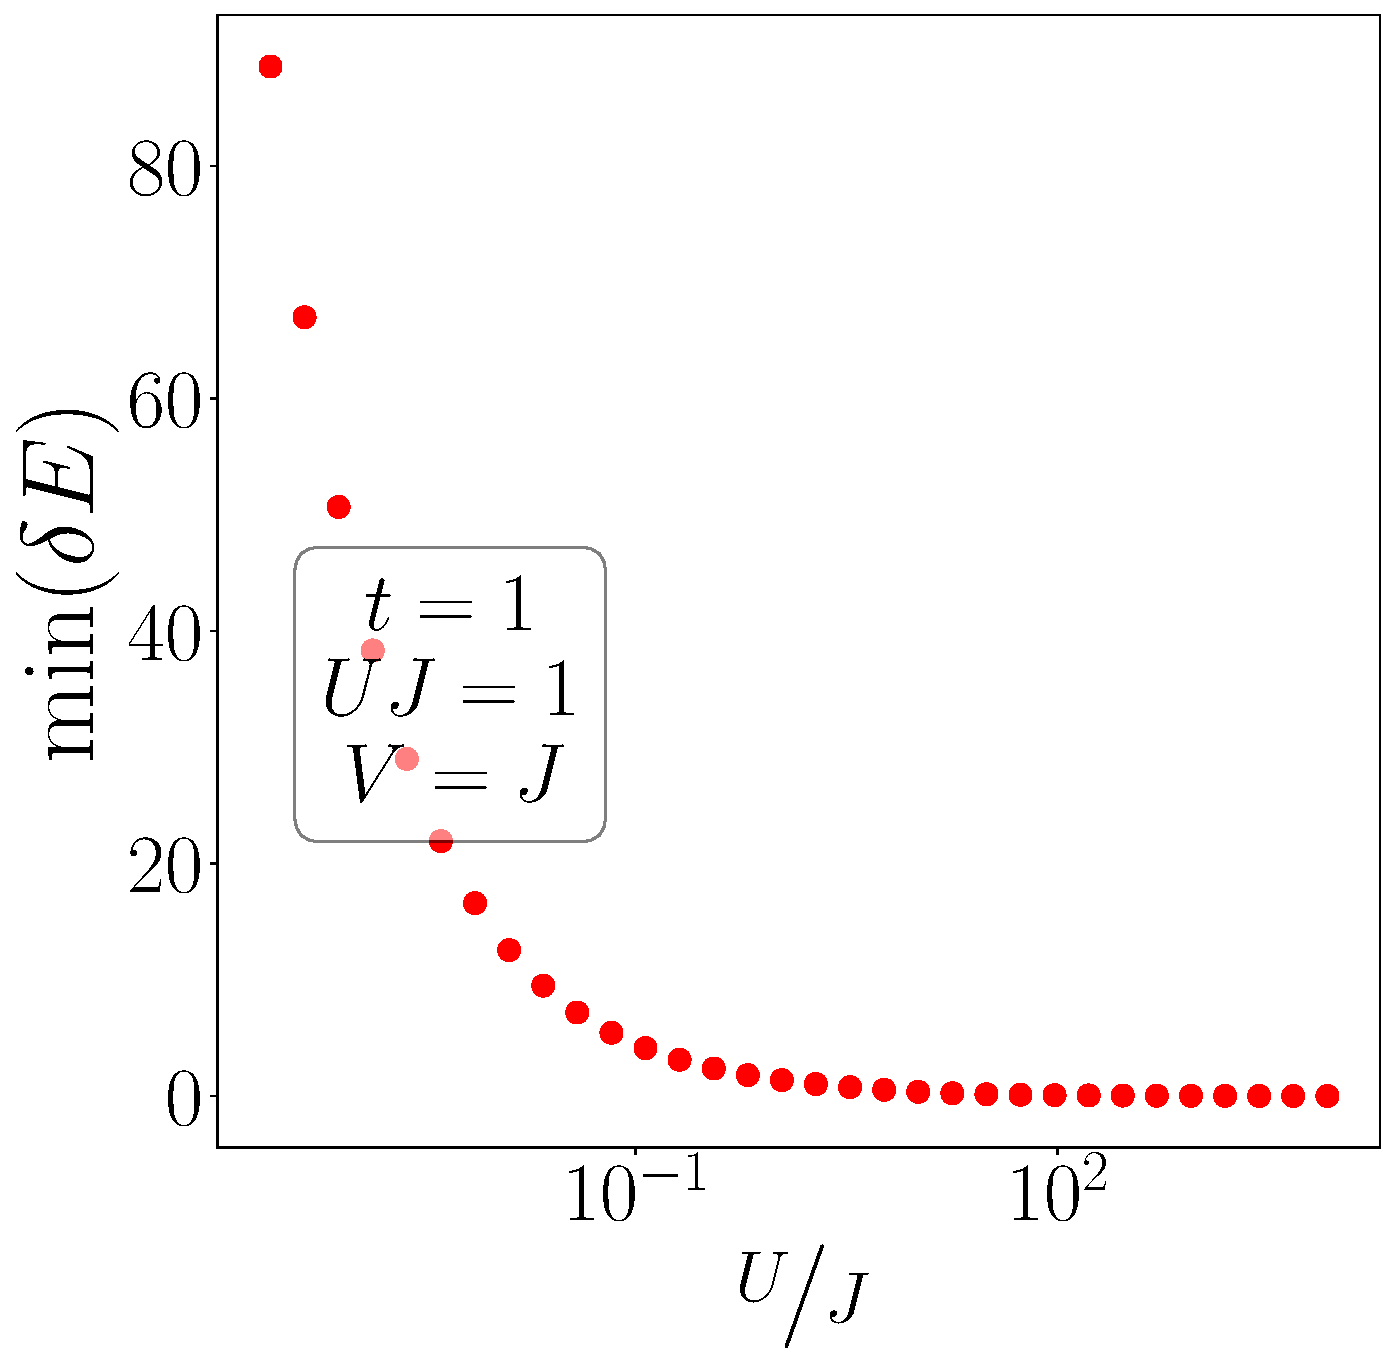
\includegraphics[width=0.32\textwidth]{../figures/gap-t=1.000,J=1_over_U,V=J,N=6,U=0.016,91.116,32.pdf}
	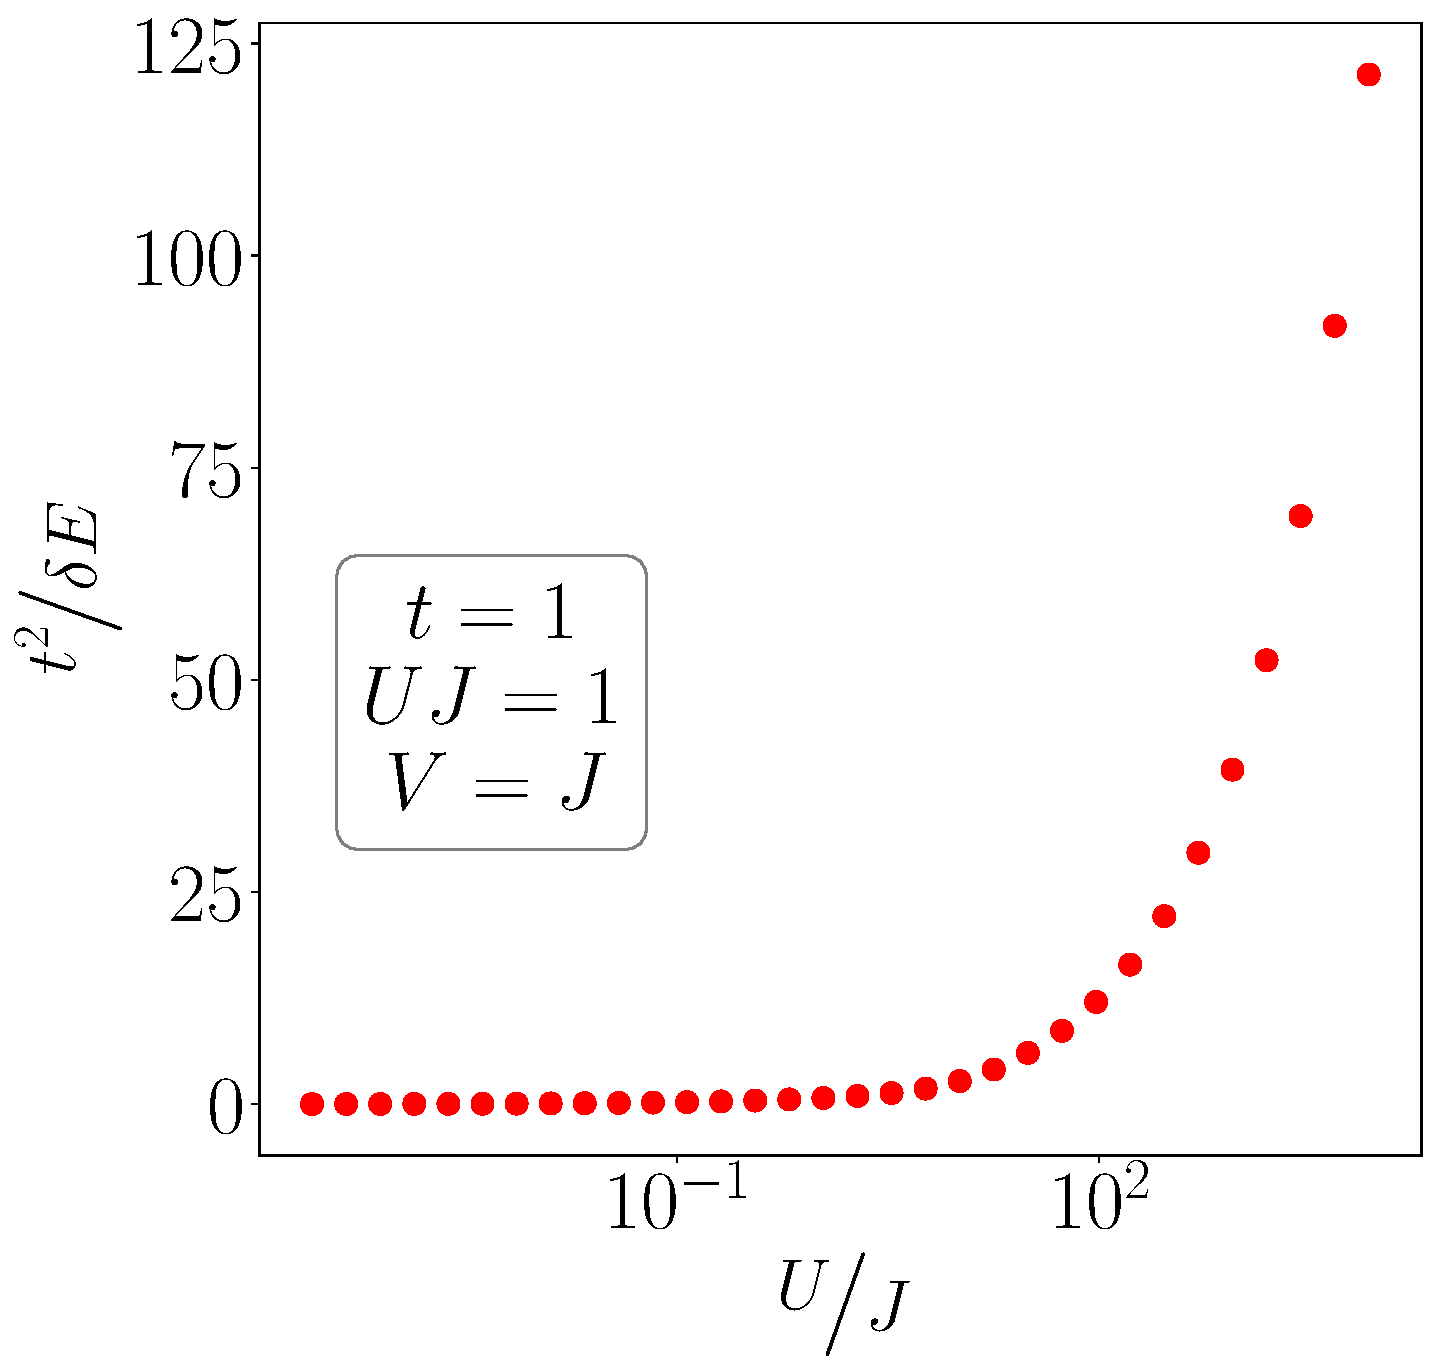
\includegraphics[width=0.32\textwidth]{../figures/par-t=1.000,J=1_over_U,V=J,N=6,U=0.016,91.116,32.pdf}
	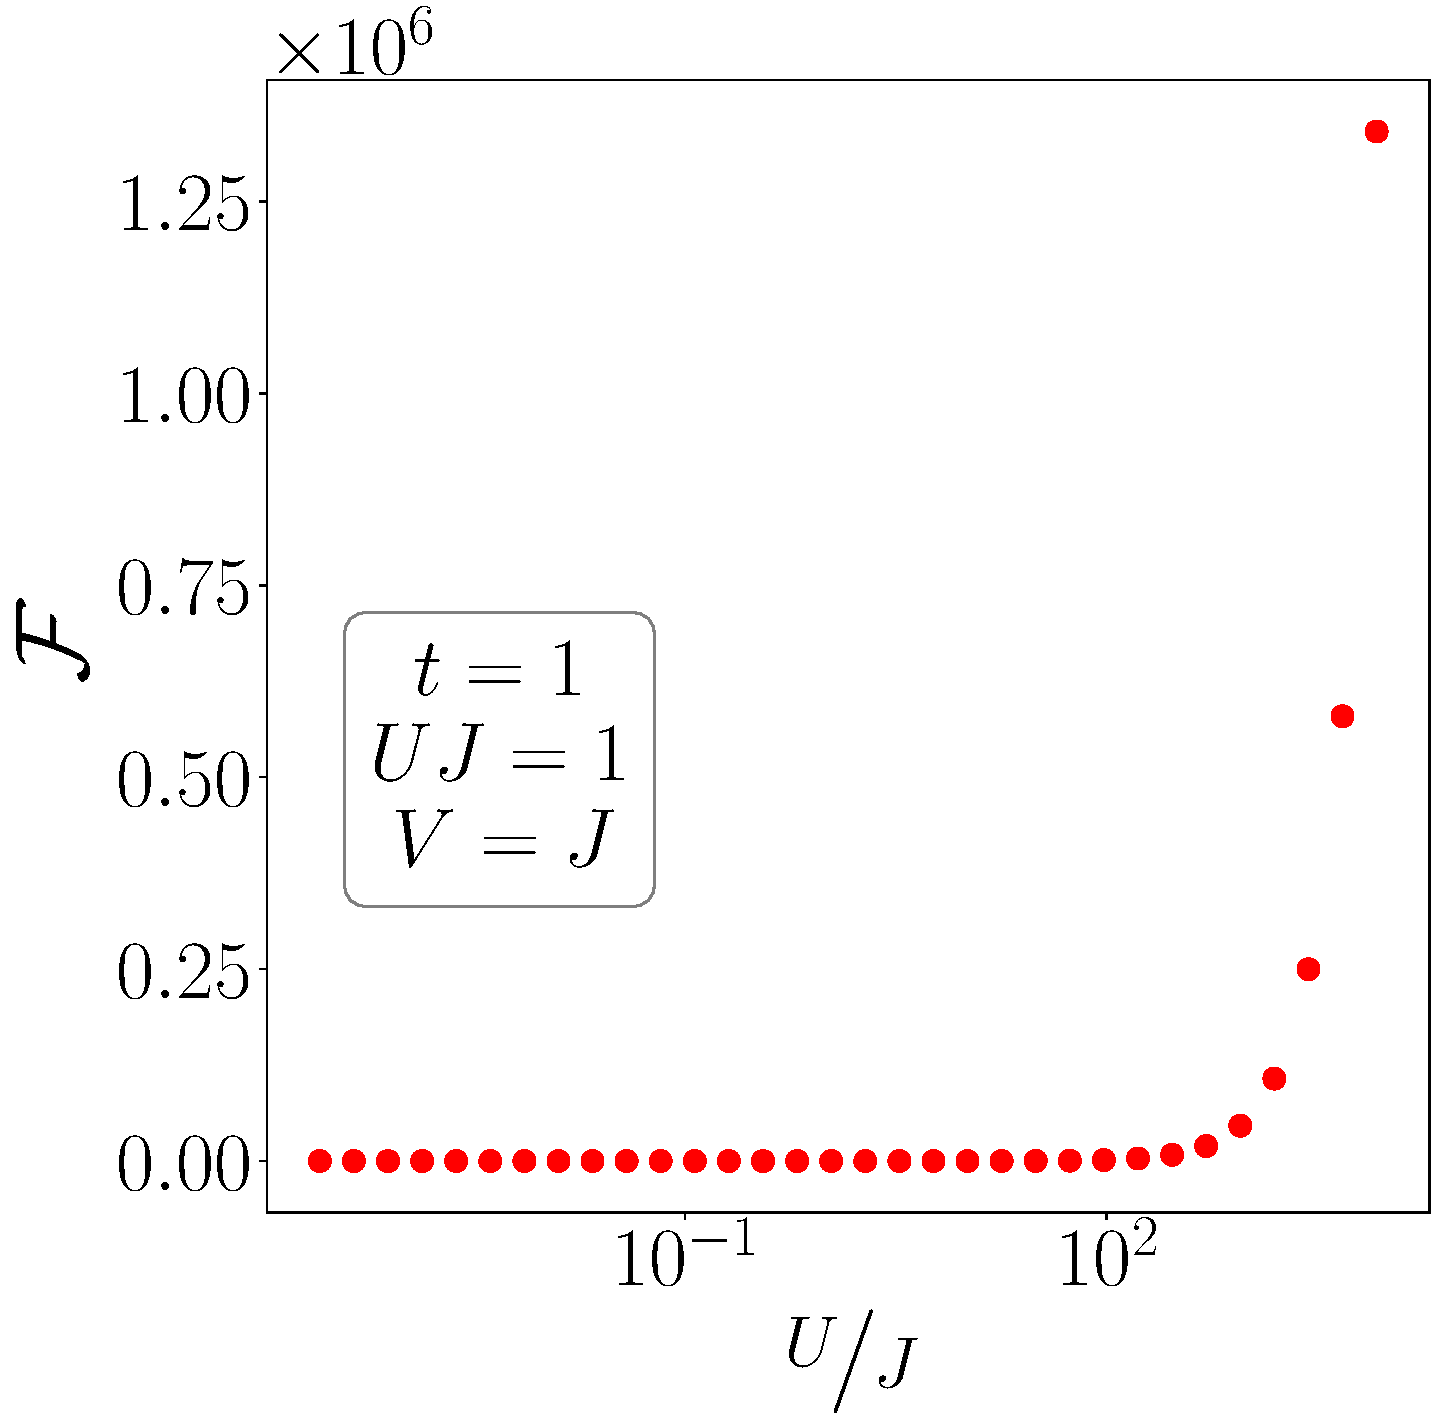
\includegraphics[width=0.32\textwidth]{../figures/lfl-t=1.000,J=1_over_U,V=J,N=6,U=0.016,91.116,32.pdf}
\end{center}
The vanishing of the gap and the growth of the small parameter indicates the breakdown of perturbation theory around the singlet; this simply shows that there is a degeneracy in the local moment regime, and the effective Hamiltonian will have to be obtained using degenerate perturbation theory. The presence of degeneracy also suggests that the effective Hamiltonian will be of the non-Fermi liquid type.

\subsection*{\(k-\)space correlations within the Kondo cloud}
\begin{center}
	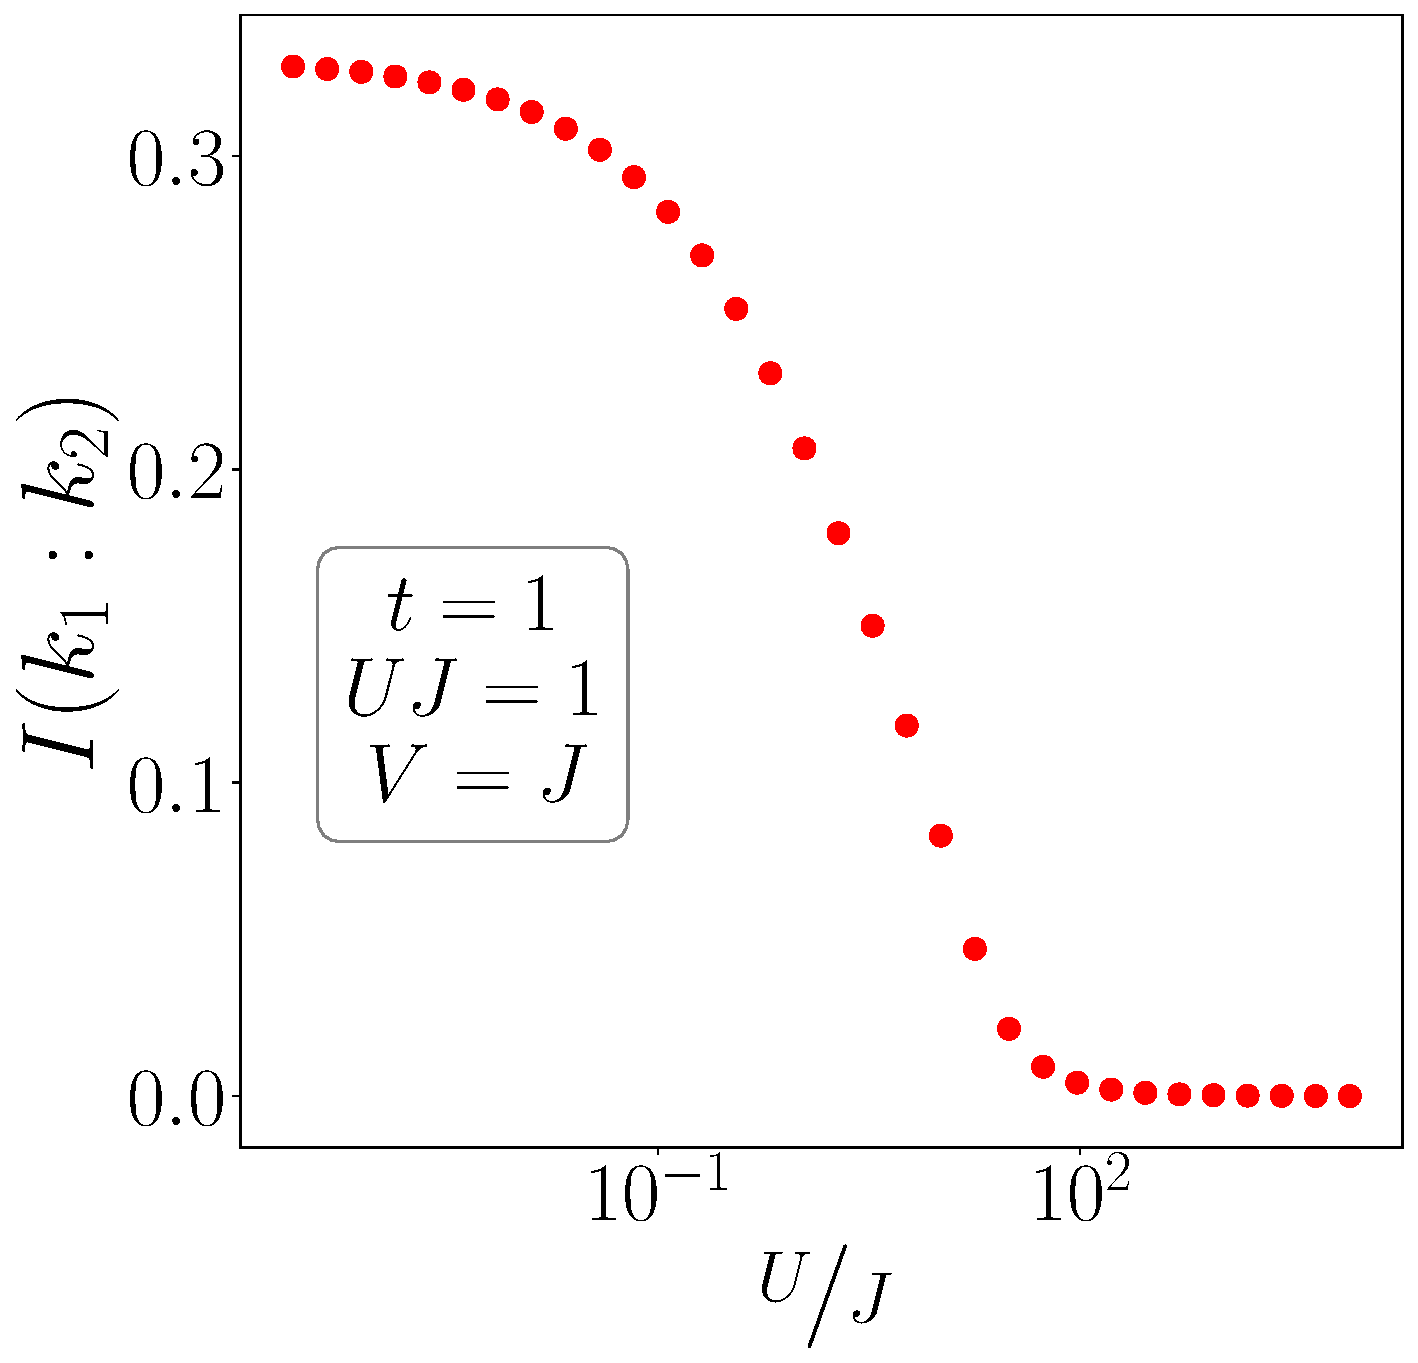
\includegraphics[width=0.32\textwidth]{../figures/corr-k-t=1.000,J=1_over_U,V=J,N=6,U=0.016,91.116,32.pdf}
	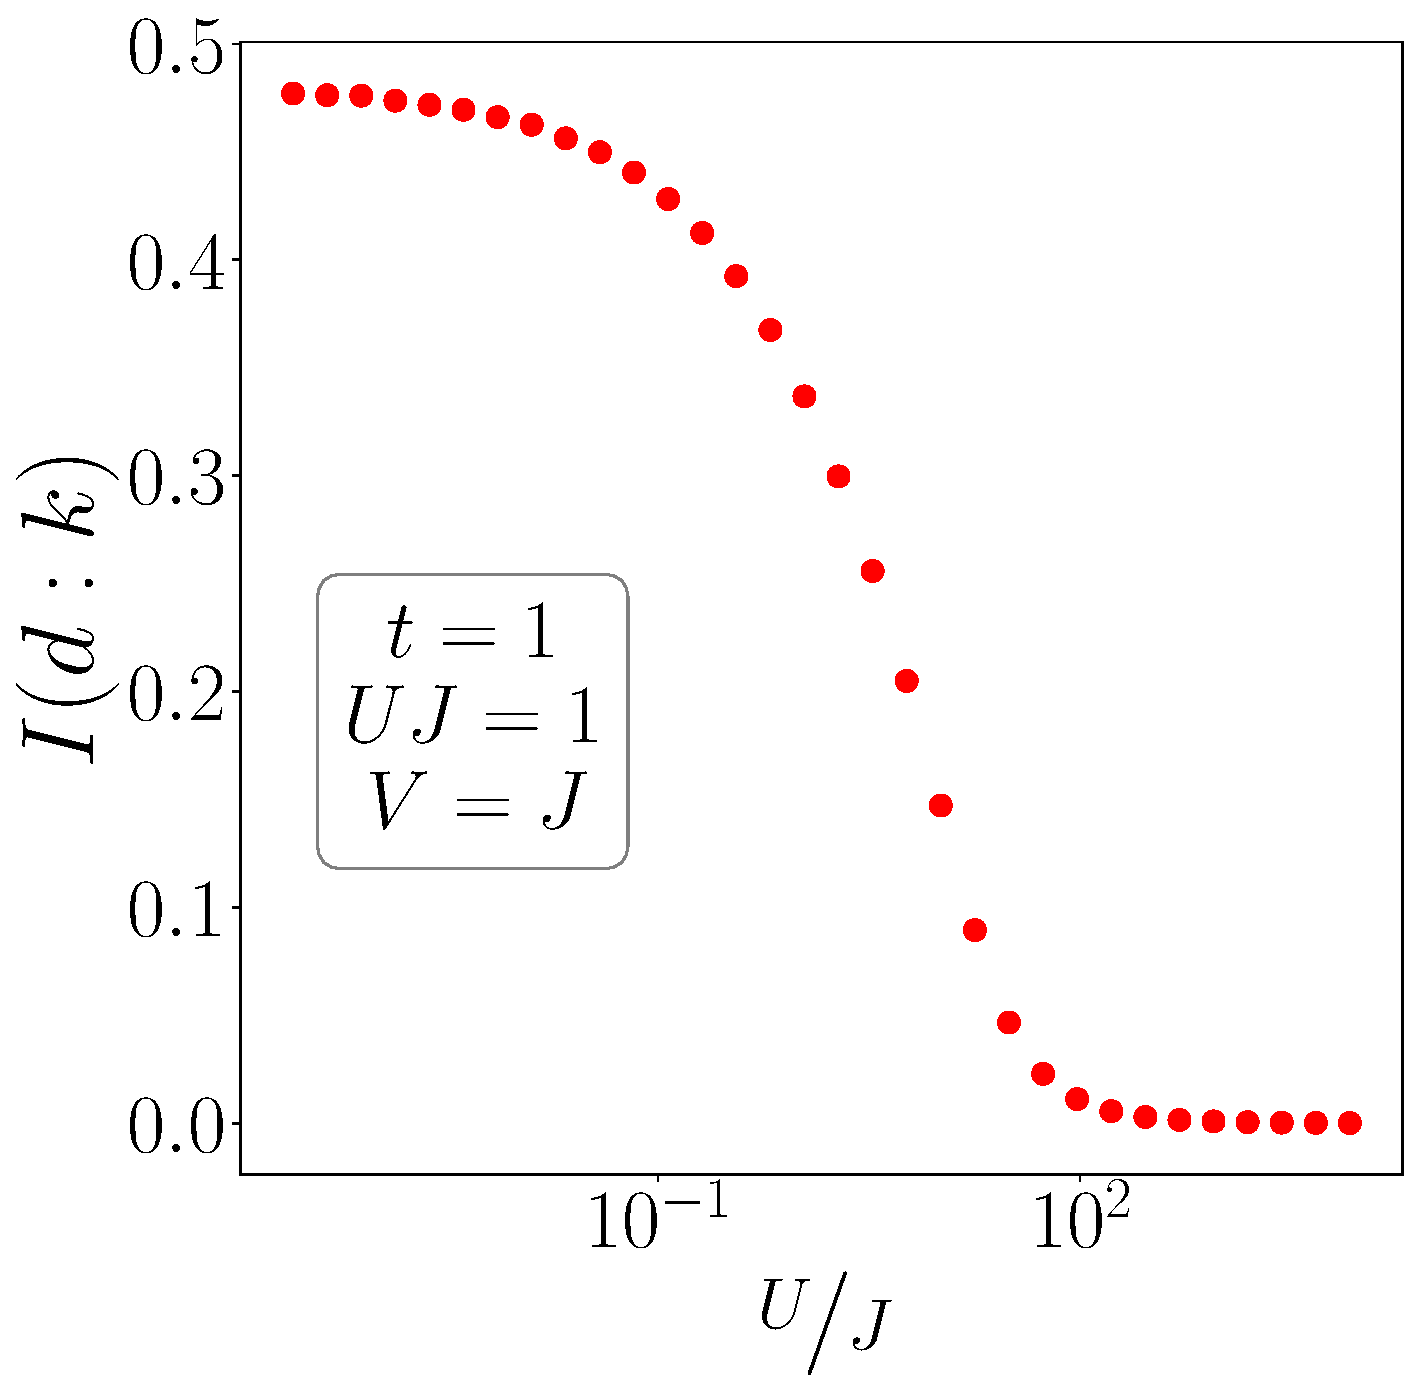
\includegraphics[width=0.32\textwidth]{../figures/mi-dk-t=1.000,J=1_over_U,V=J,N=6,U=0.016,91.116,32.pdf}
	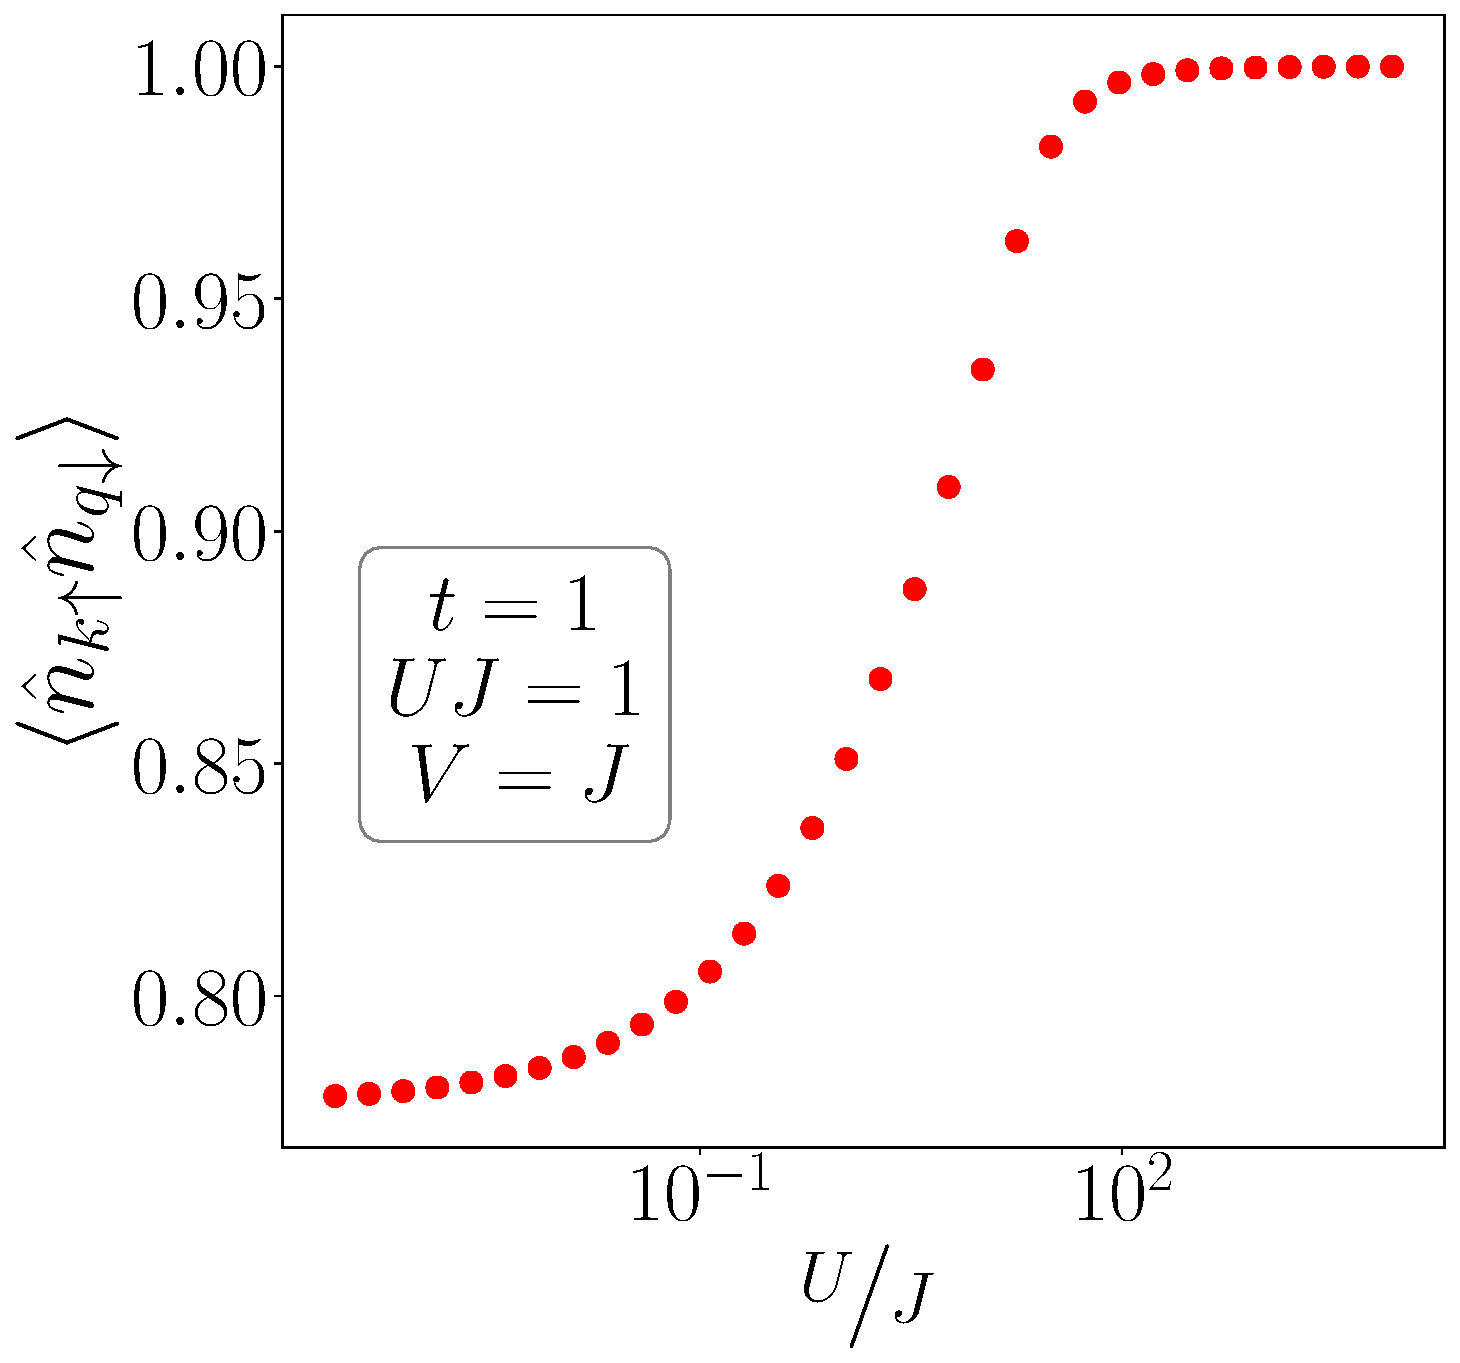
\includegraphics[width=0.32\textwidth]{../figures/corr-k-diag-t=1.000,J=1_over_U,V=J,N=6,U=0.016,91.116,32.pdf}
	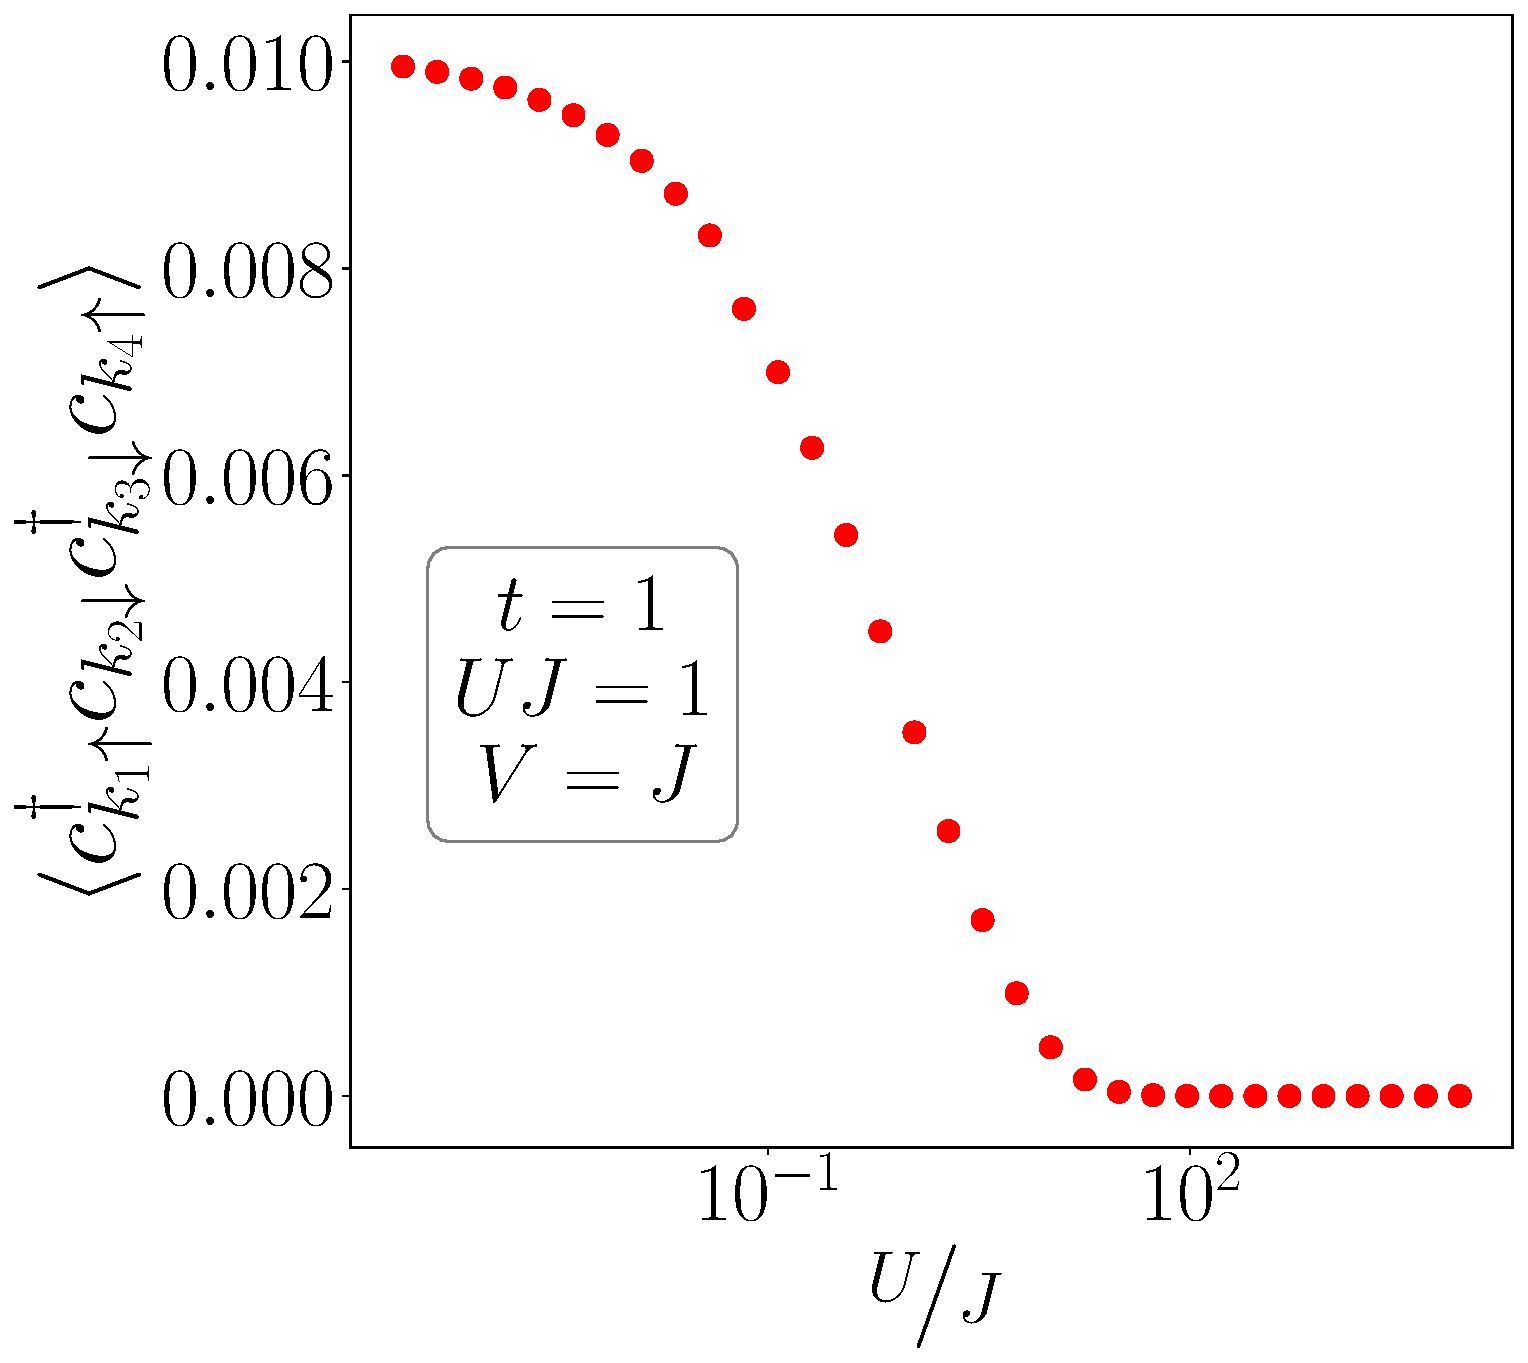
\includegraphics[width=0.32\textwidth]{../figures/corr-k-od-t=1.000,J=1_over_U,V=J,N=6,U=0.016,91.116,32.pdf}
\end{center}
The vanishing of the Kondo cloud at large \(U/J\) is clear indication of the destruction of the Kondo cloud and the breakdown of screening. Non-zero mutual information indicates an (impurity-mediated) interaction between the \(k-\)states of the conduction bath; seen differently, it is this interaction that is responsively for the screening of the impurity. The disappearance of the mutual information is indicative of the disappearance of this interaction.

\subsection*{Mutual information between various real space members}
\begin{center}
	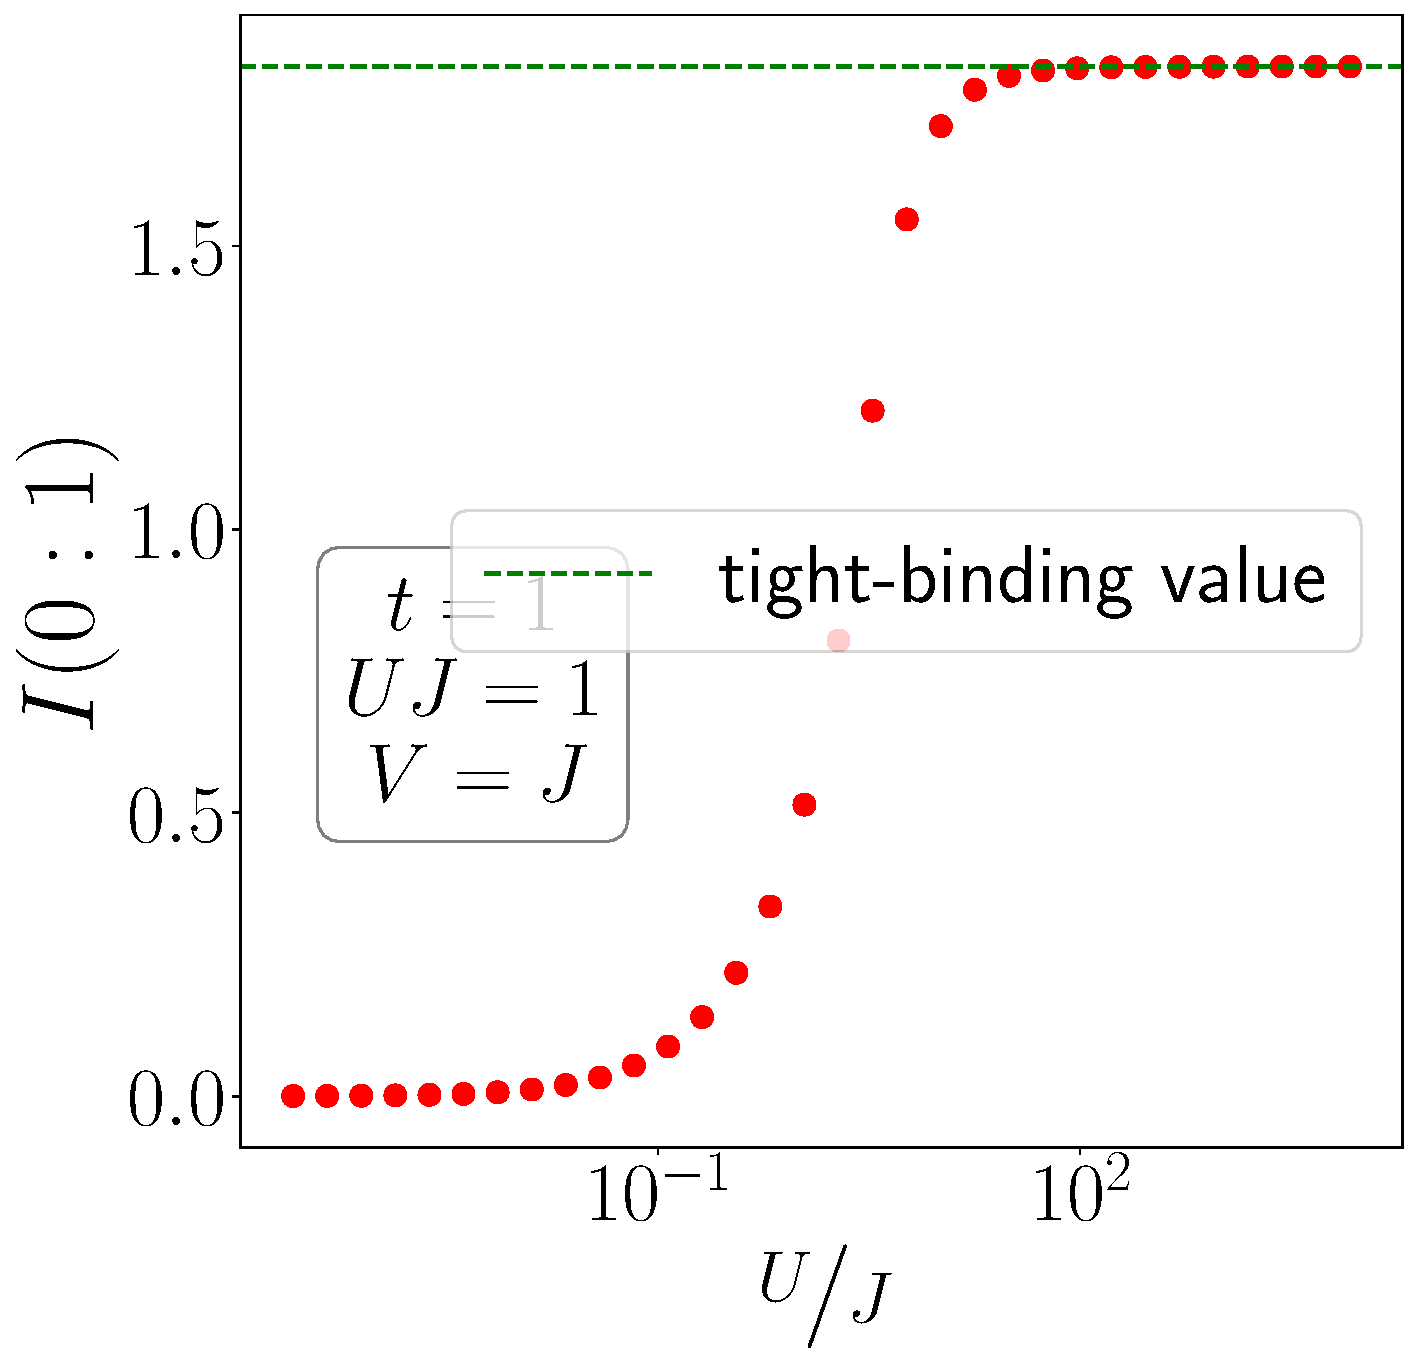
\includegraphics[width=0.32\textwidth]{../figures/mi-01-t=1.000,J=1_over_U,V=J,N=6,U=0.016,91.116,32.pdf}
	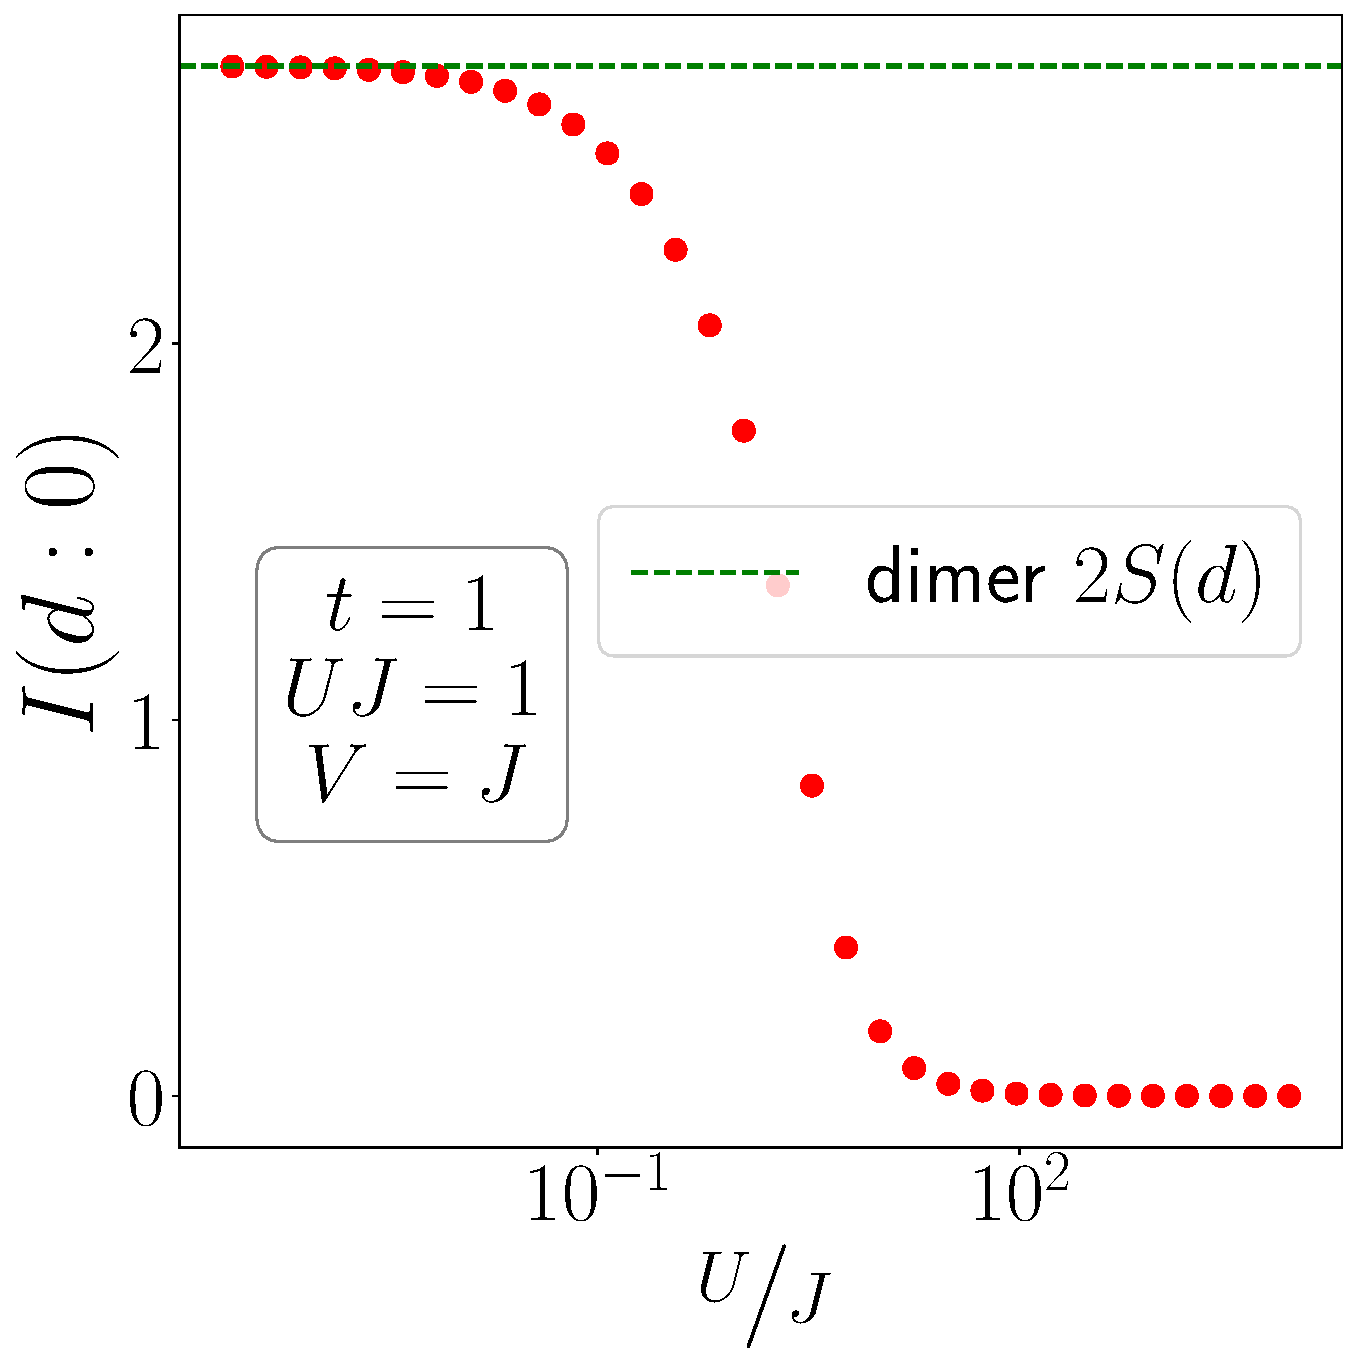
\includegraphics[width=0.32\textwidth]{../figures/mi-d0-t=1.000,J=1_over_U,V=J,N=6,U=0.016,91.116,32.pdf}
	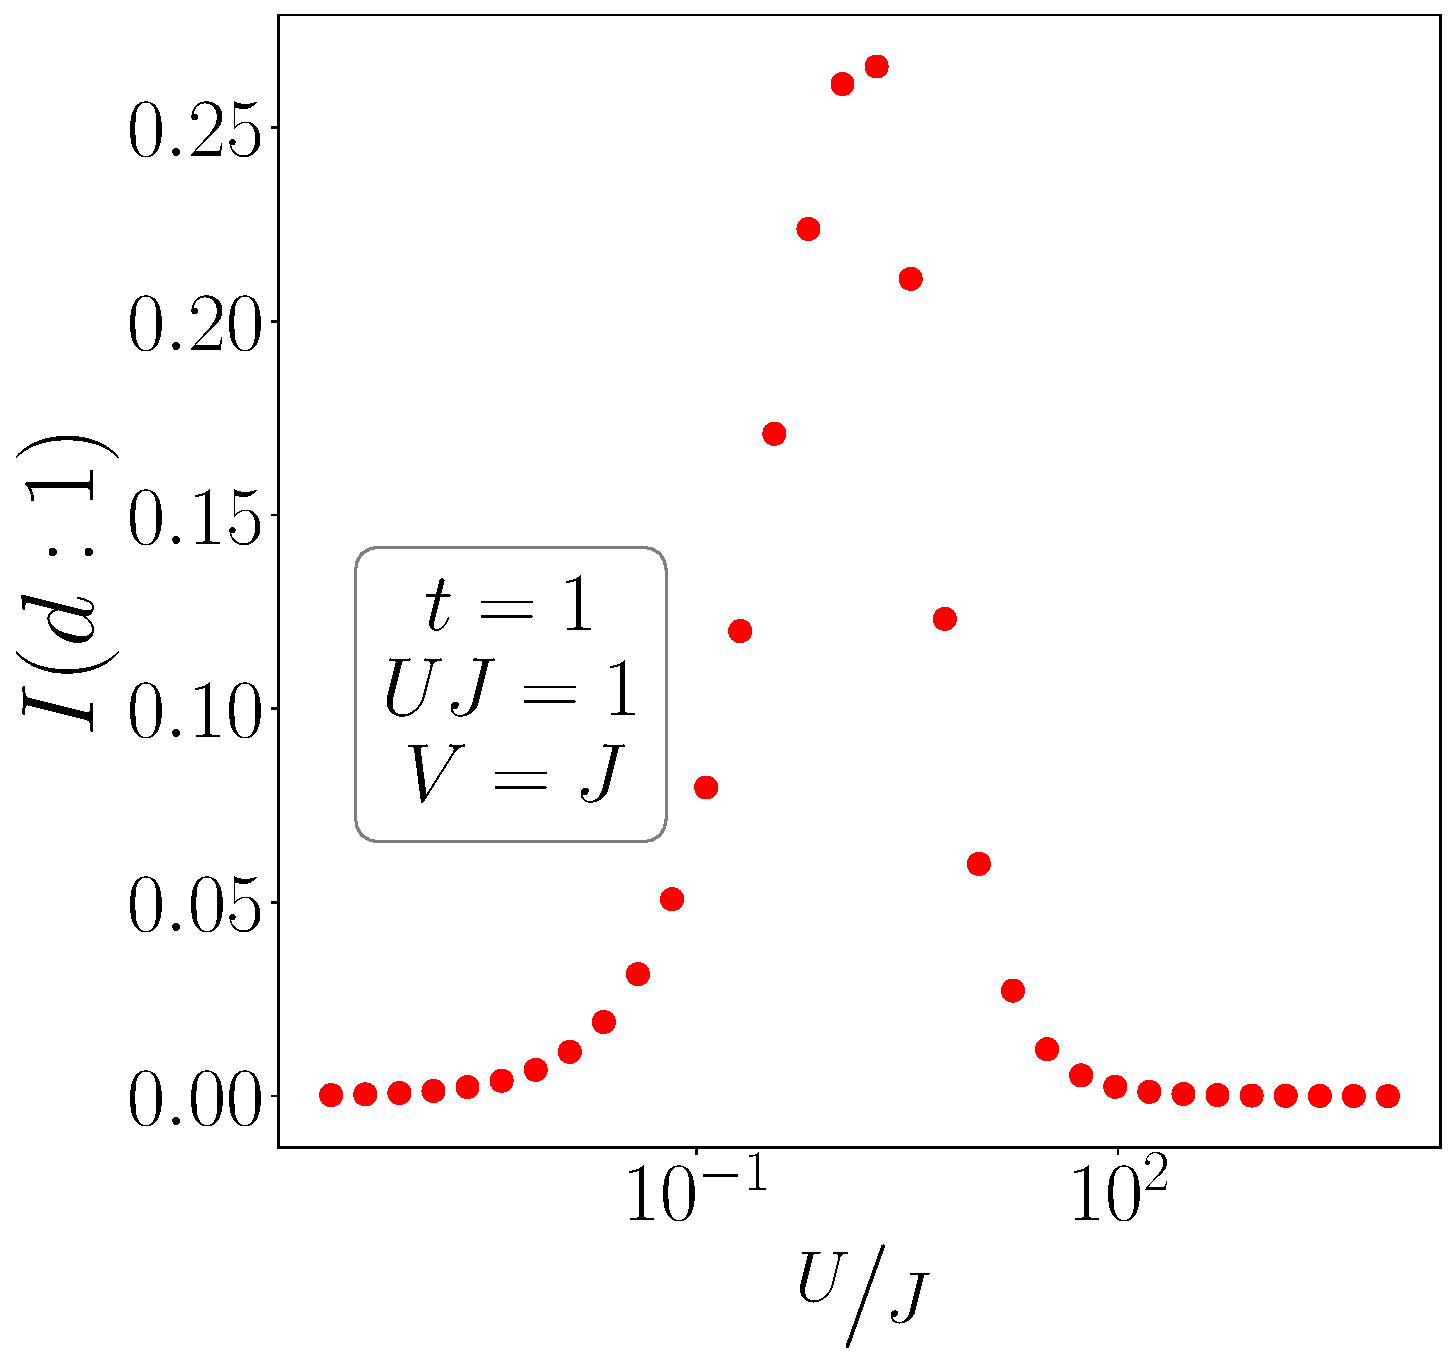
\includegraphics[width=0.32\textwidth]{../figures/mi-d1-t=1.000,J=1_over_U,V=J,N=6,U=0.016,91.116,32.pdf}
\end{center}
The impurity-zeroth site mutual information \(I(d:0)\) remains unchanged at the maximum for an appreciable range of values, and this shows the stability of the singlet. Meanwhile, the mutual information between the zeroth site and the site nearest to it (\(I(0:1)\)) grows, because when the singlet weakens, the zeroth site is able to entangle more with the other sites. It finally saturates to its maximum value, which is the value produced as result of the tight-binding hopping. The mutual information between the impurity and sites beyond the zeroth site (\(I(d:1)\)) show a non-monotonic behaviour; it first increases as the entanglement that was initially restricted to just the impurity and the zeroth sites begins "seeping" into the other sites as well. Beyond a critical value of \(U/J\), \(I(d:1)\) starts dropping, because the entanglement has now mostly shifted out of the zero mode and into the conduction bath.

\subsection*{Impurity entanglement entropy and spin-spin correlations}

\begin{center}
	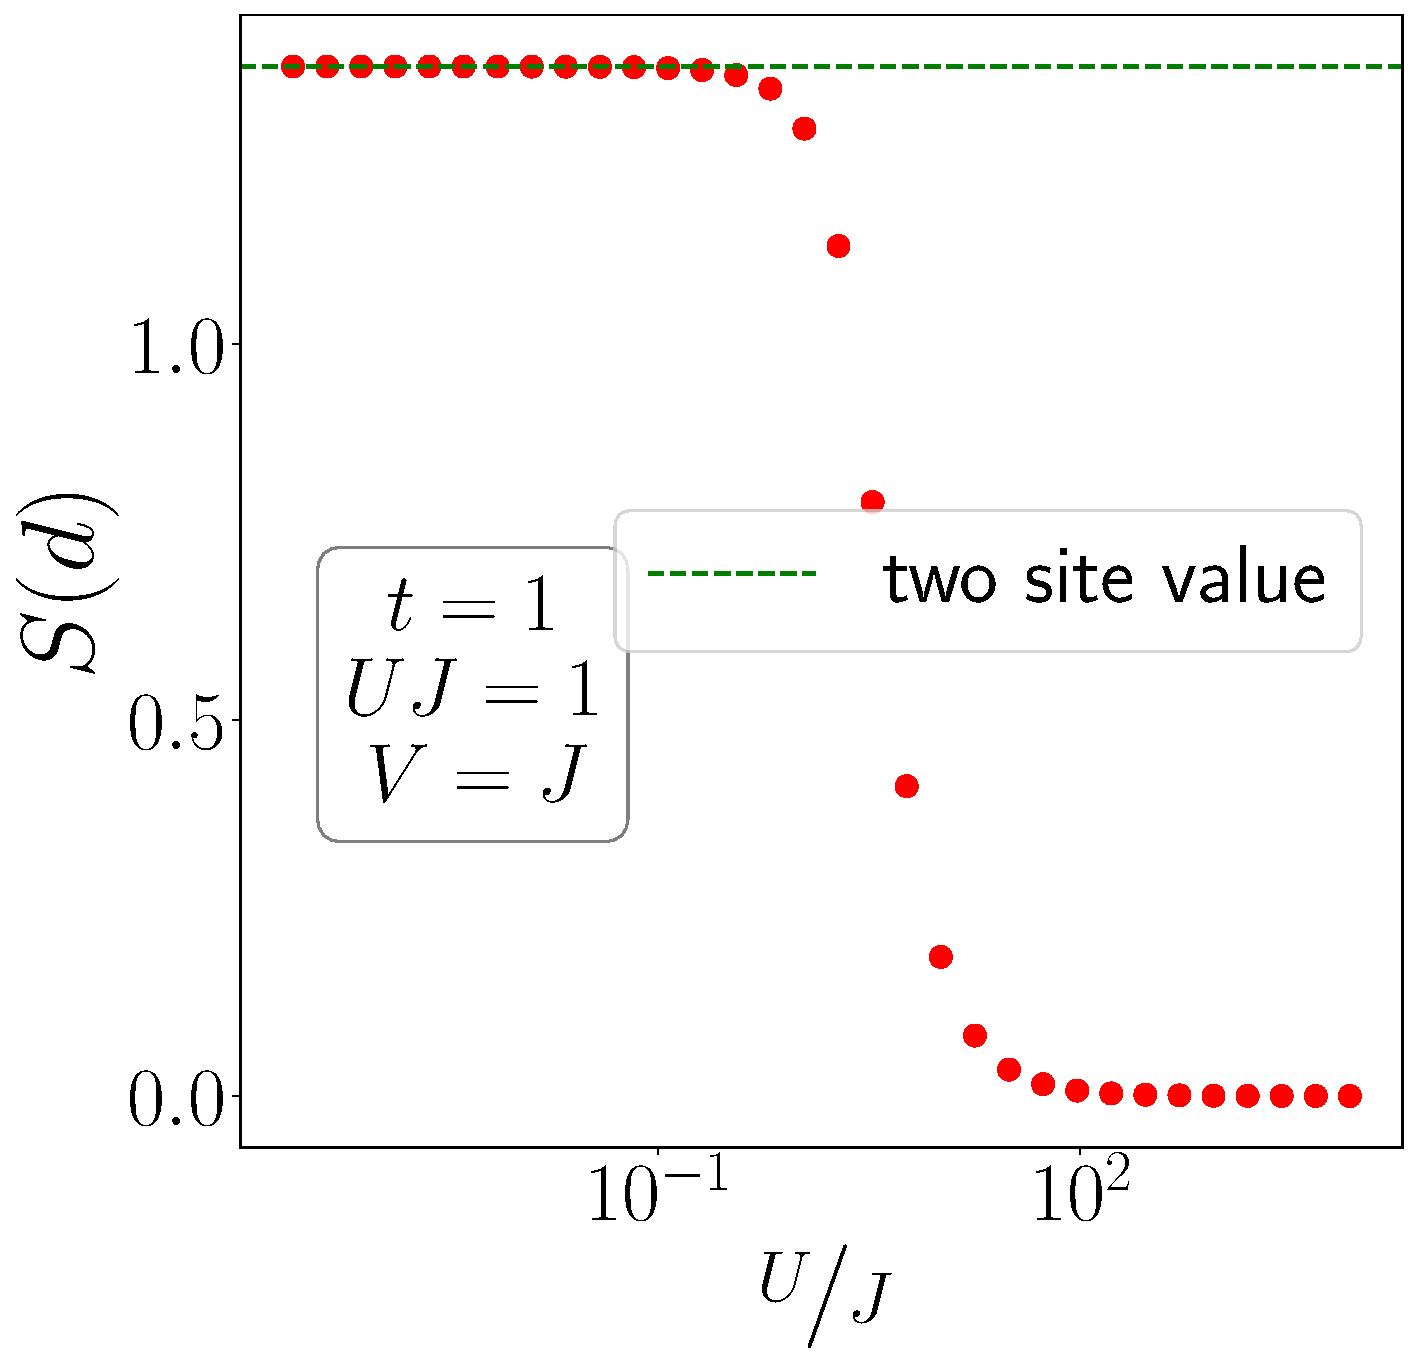
\includegraphics[width=0.32\textwidth]{../figures/EE-d-t=1.000,J=1_over_U,V=J,N=6,U=0.016,91.116,32.pdf}
	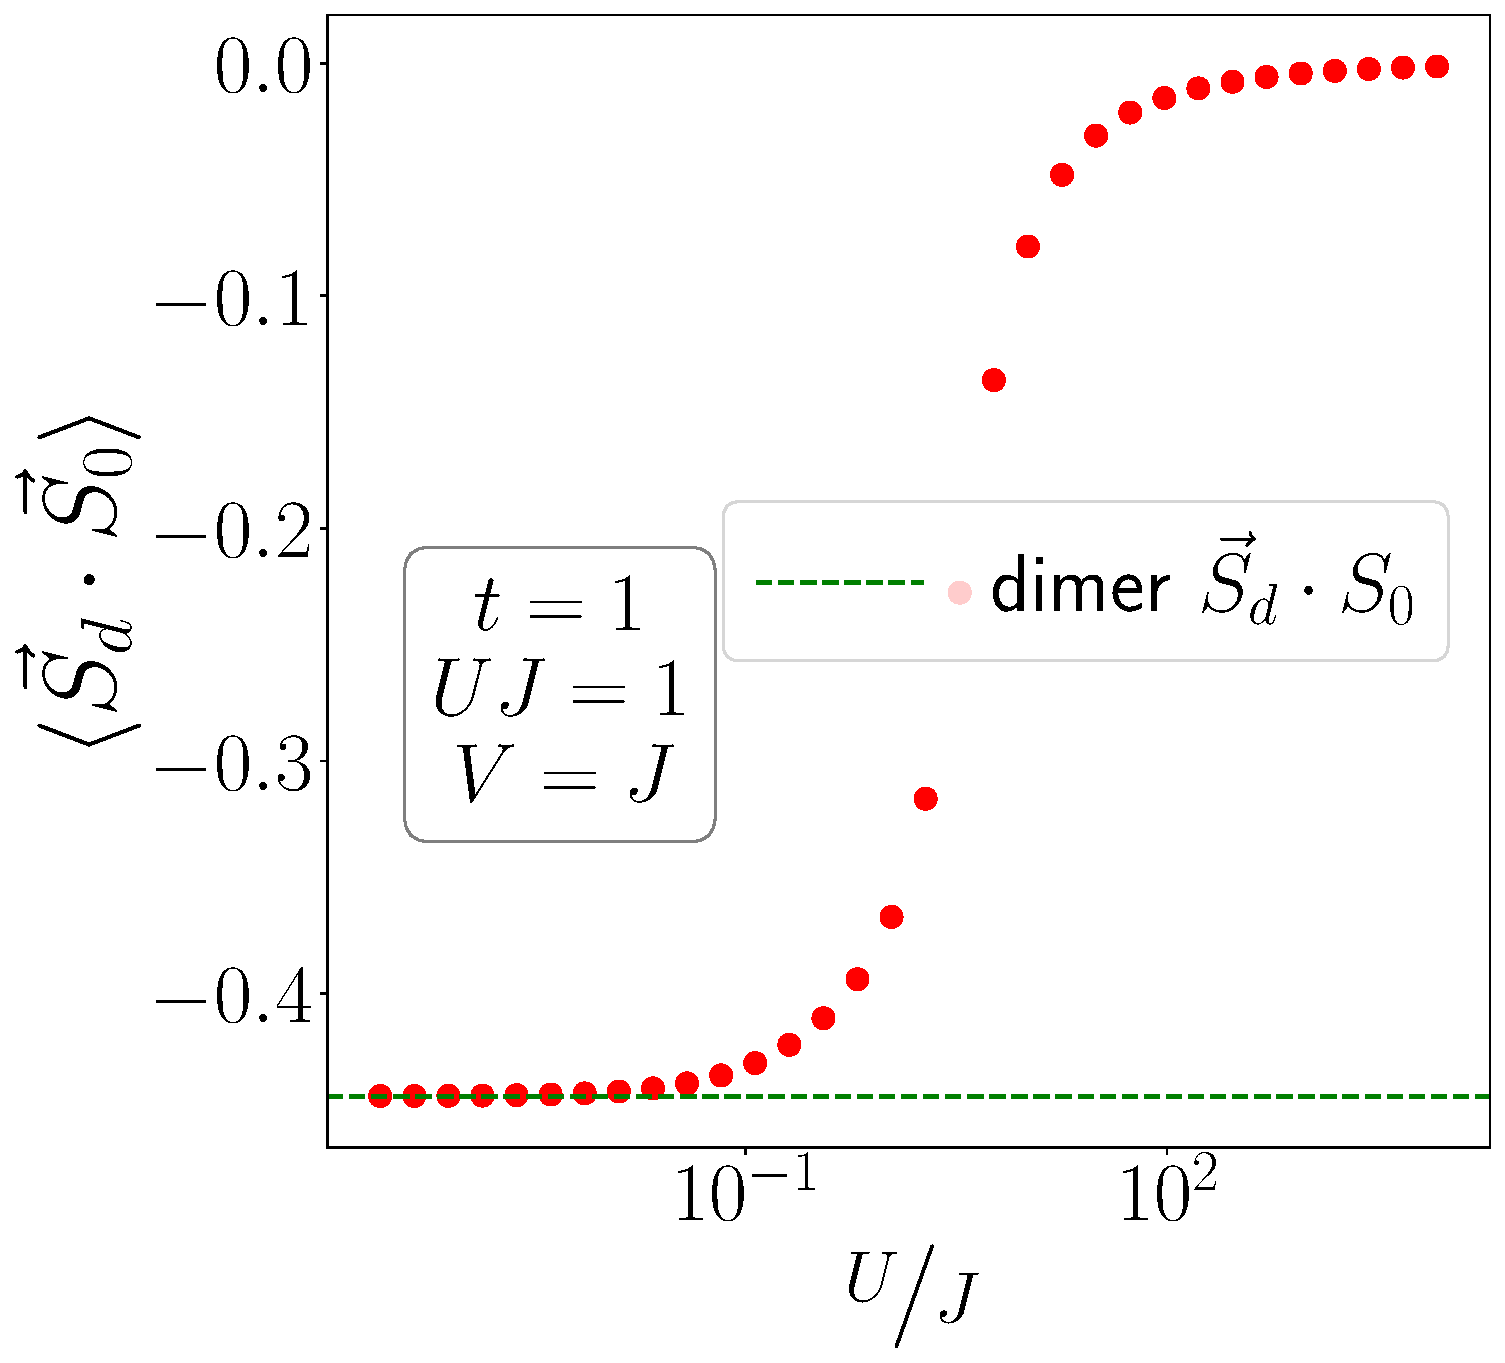
\includegraphics[width=0.32\textwidth]{../figures/corr-d0-t=1.000,J=1_over_U,V=J,N=6,U=0.016,91.116,32.pdf}
	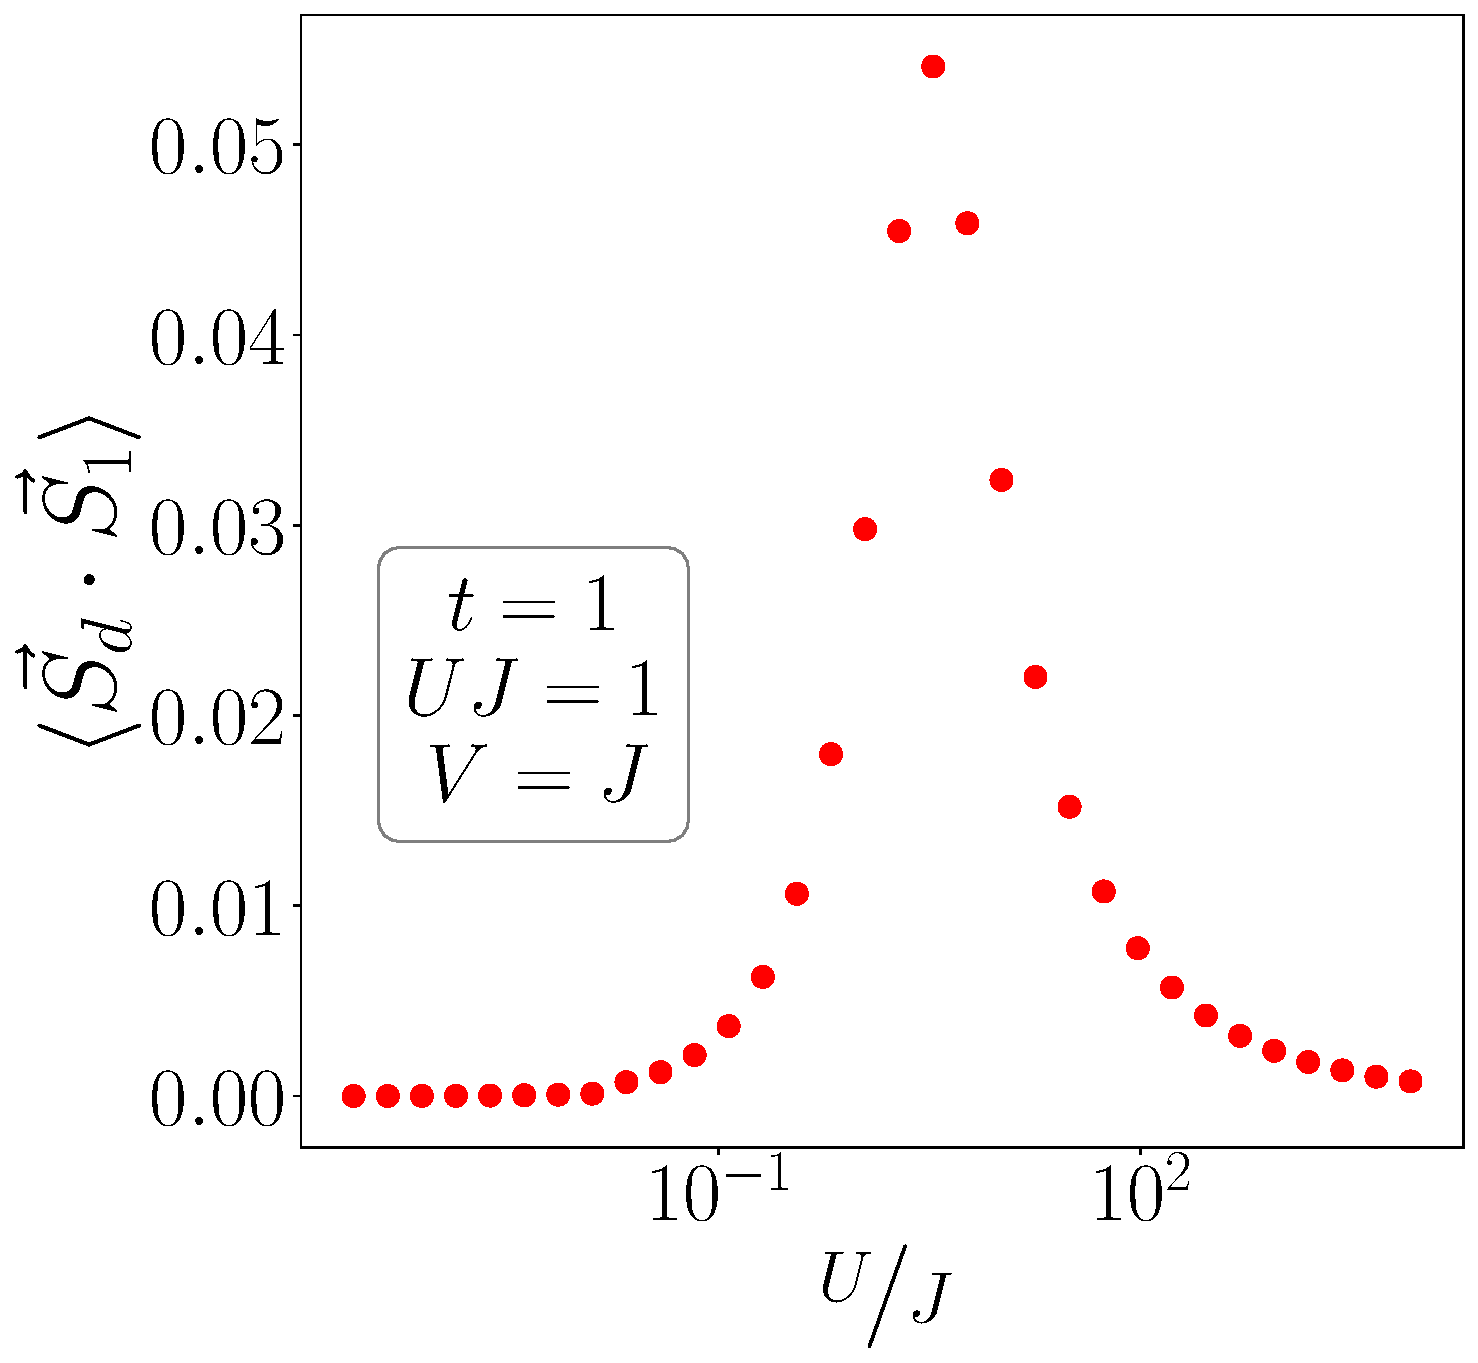
\includegraphics[width=0.32\textwidth]{../figures/corr-d1-t=1.000,J=1_over_U,V=J,N=6,U=0.016,91.116,32.pdf}
	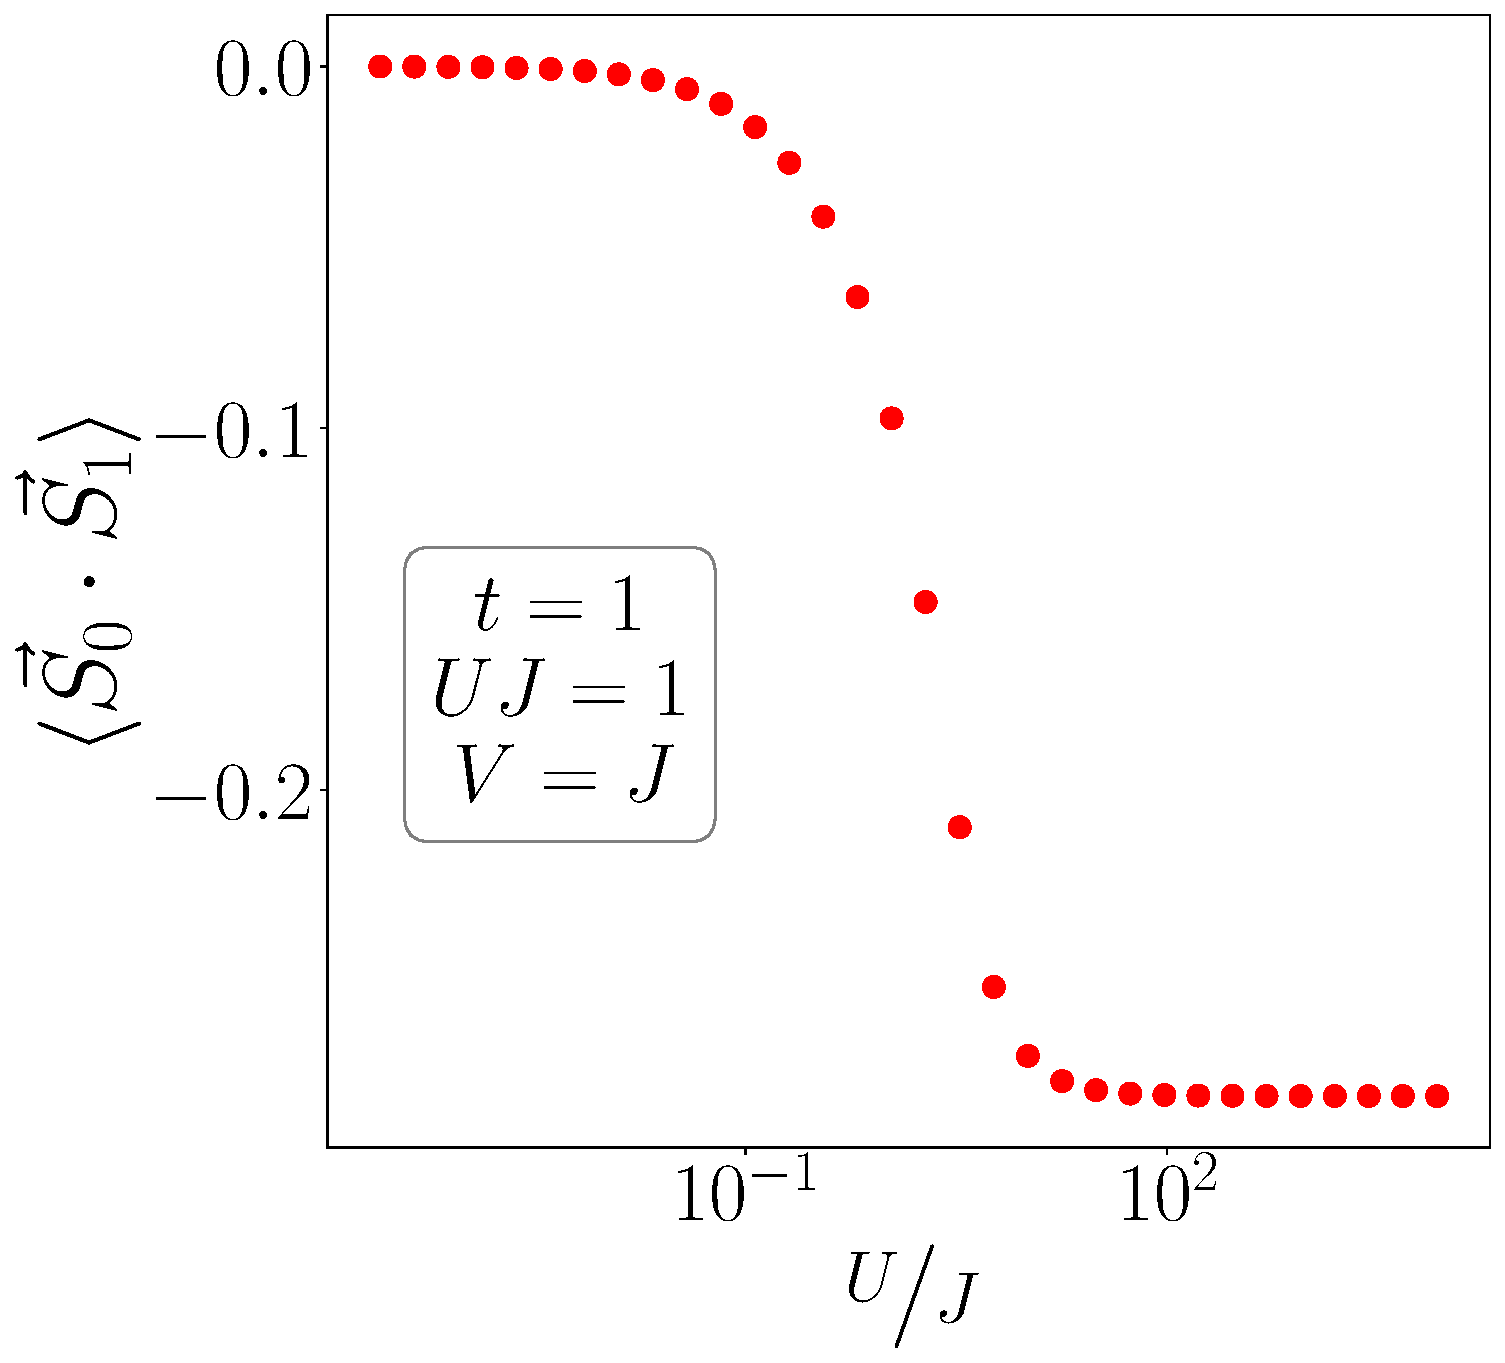
\includegraphics[width=0.32\textwidth]{../figures/r-vec-corr-01-t=1.000,J=1_over_U,V=J,N=6,U=0.016,91.116,32.pdf}
	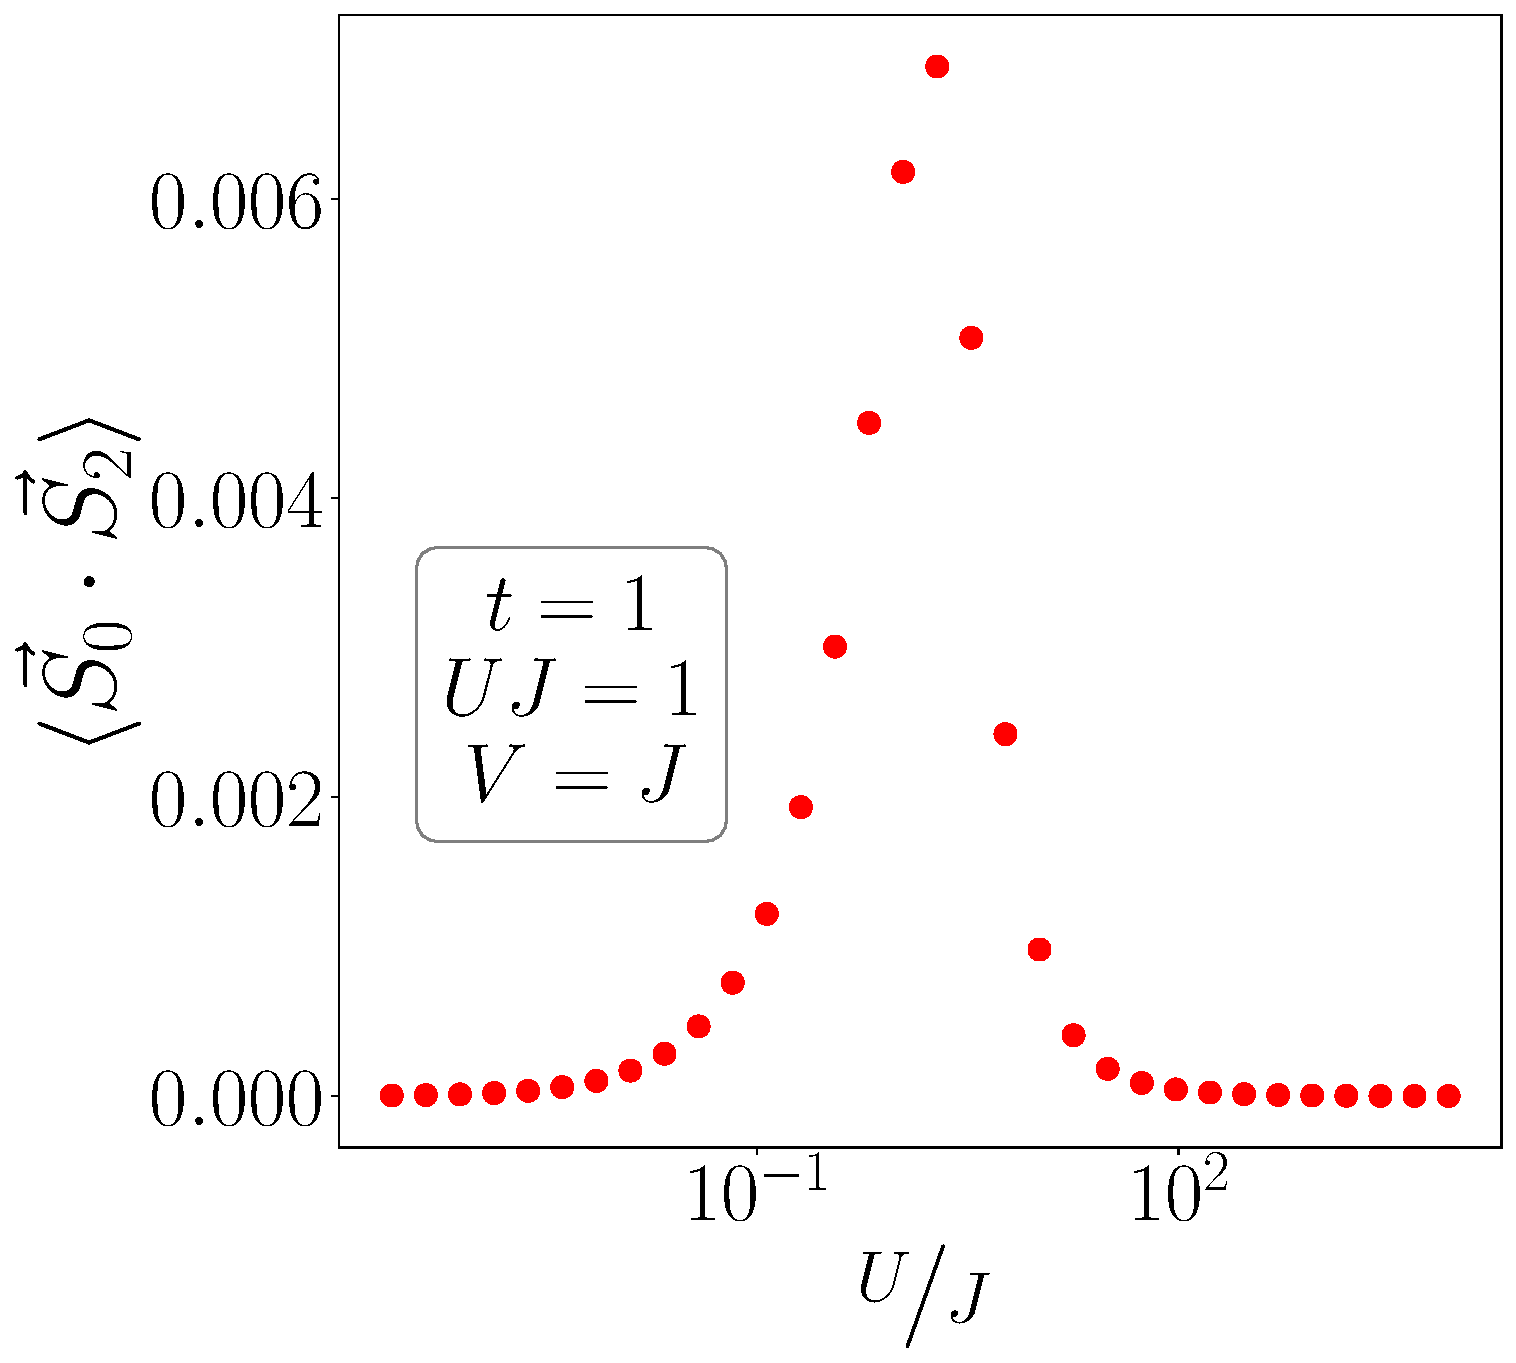
\includegraphics[width=0.32\textwidth]{../figures/r-vec-corr-02-t=1.000,J=1_over_U,V=J,N=6,U=0.016,91.116,32.pdf}
	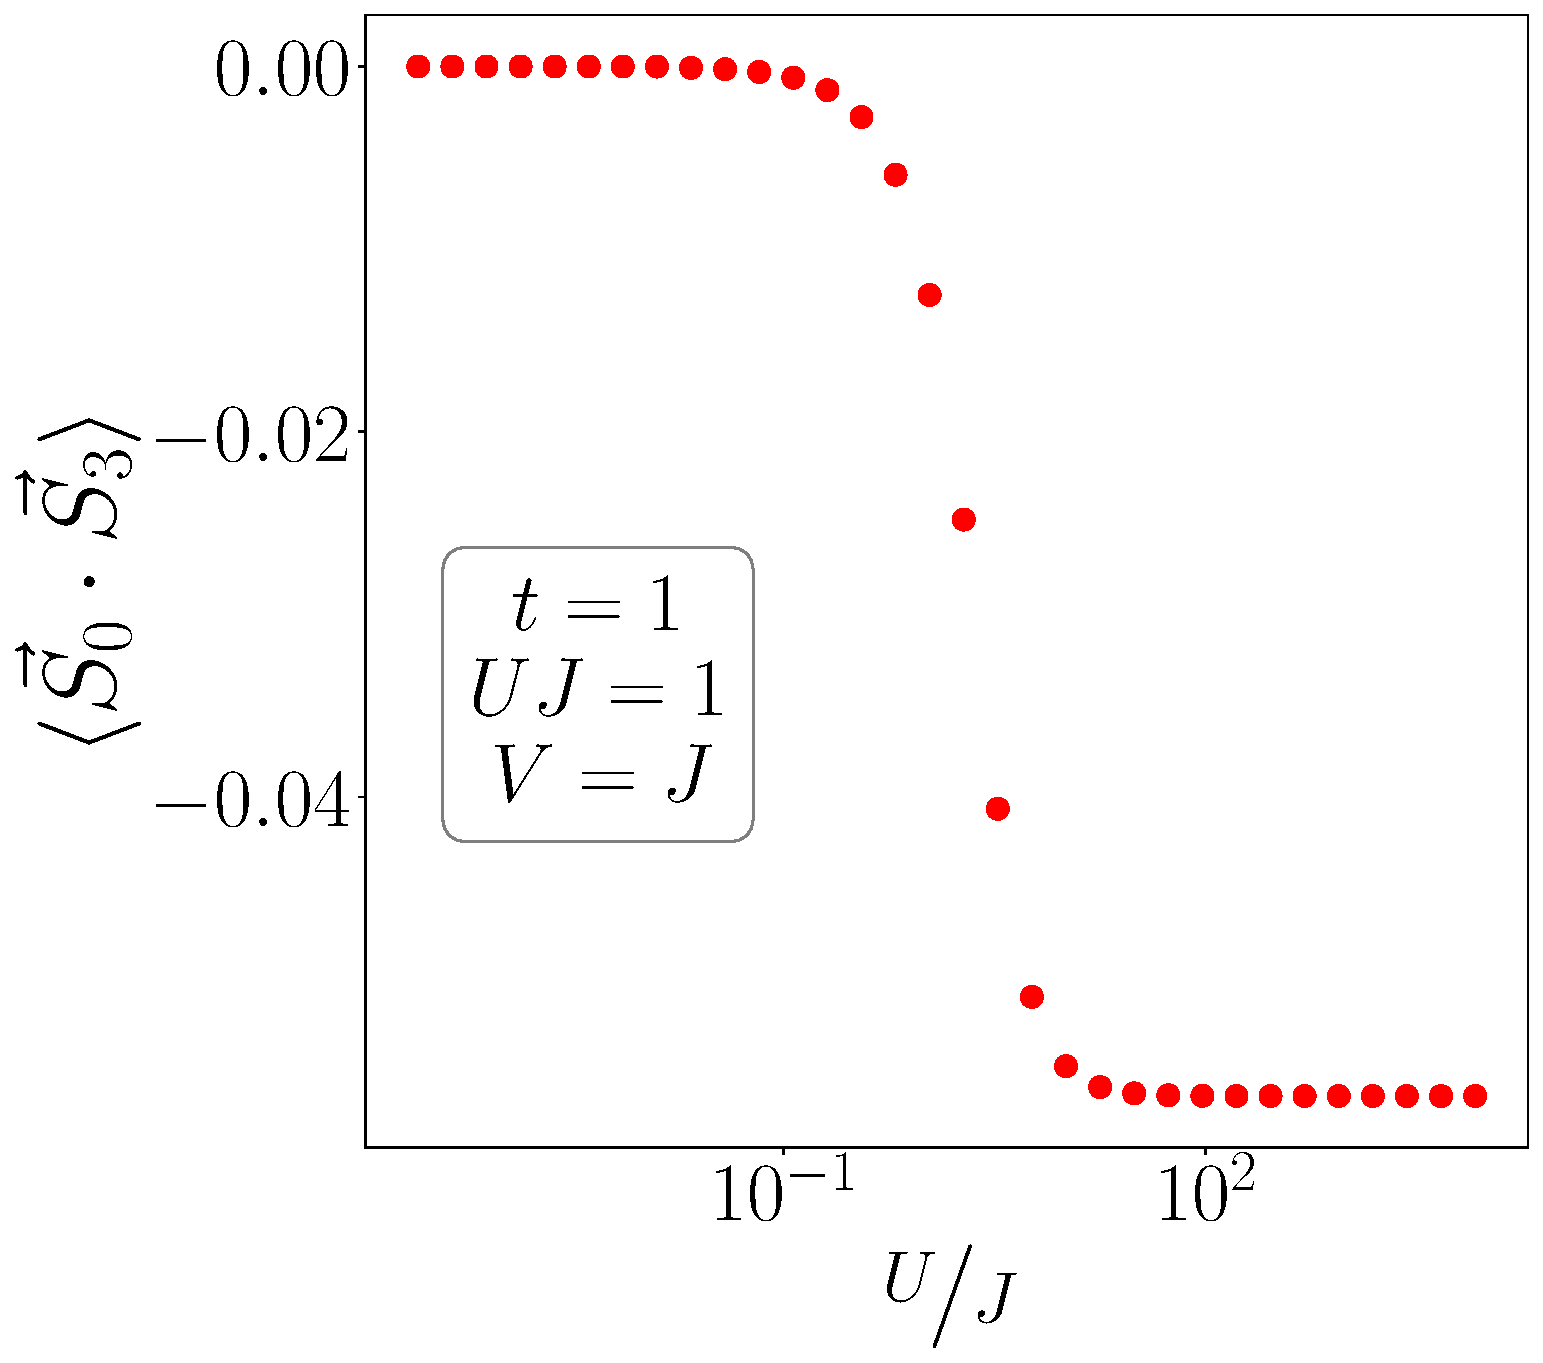
\includegraphics[width=0.32\textwidth]{../figures/r-vec-corr-03-t=1.000,J=1_over_U,V=J,N=6,U=0.016,91.116,32.pdf}

\end{center}

The von-Neumann entanglement entropy \(S(d)\) of the impurity shows pretty straightforward behaviour. It is maximum for \(U \ll J\) because it is in a singlet configuration. For \(U \gg J\), the singlet weakens and the impurity begins to decouple from the bath, leading to a reduction in \(S(d)\). At sufficiently low values of \(J/U\), the impurity decouples from the zeroth site and the total system can be factorised into a local moment in product with a tight-binding chain, so that the impurity site will now have zero entanglement entropy.

\subsection*{Real-space correlations}
\begin{center}
	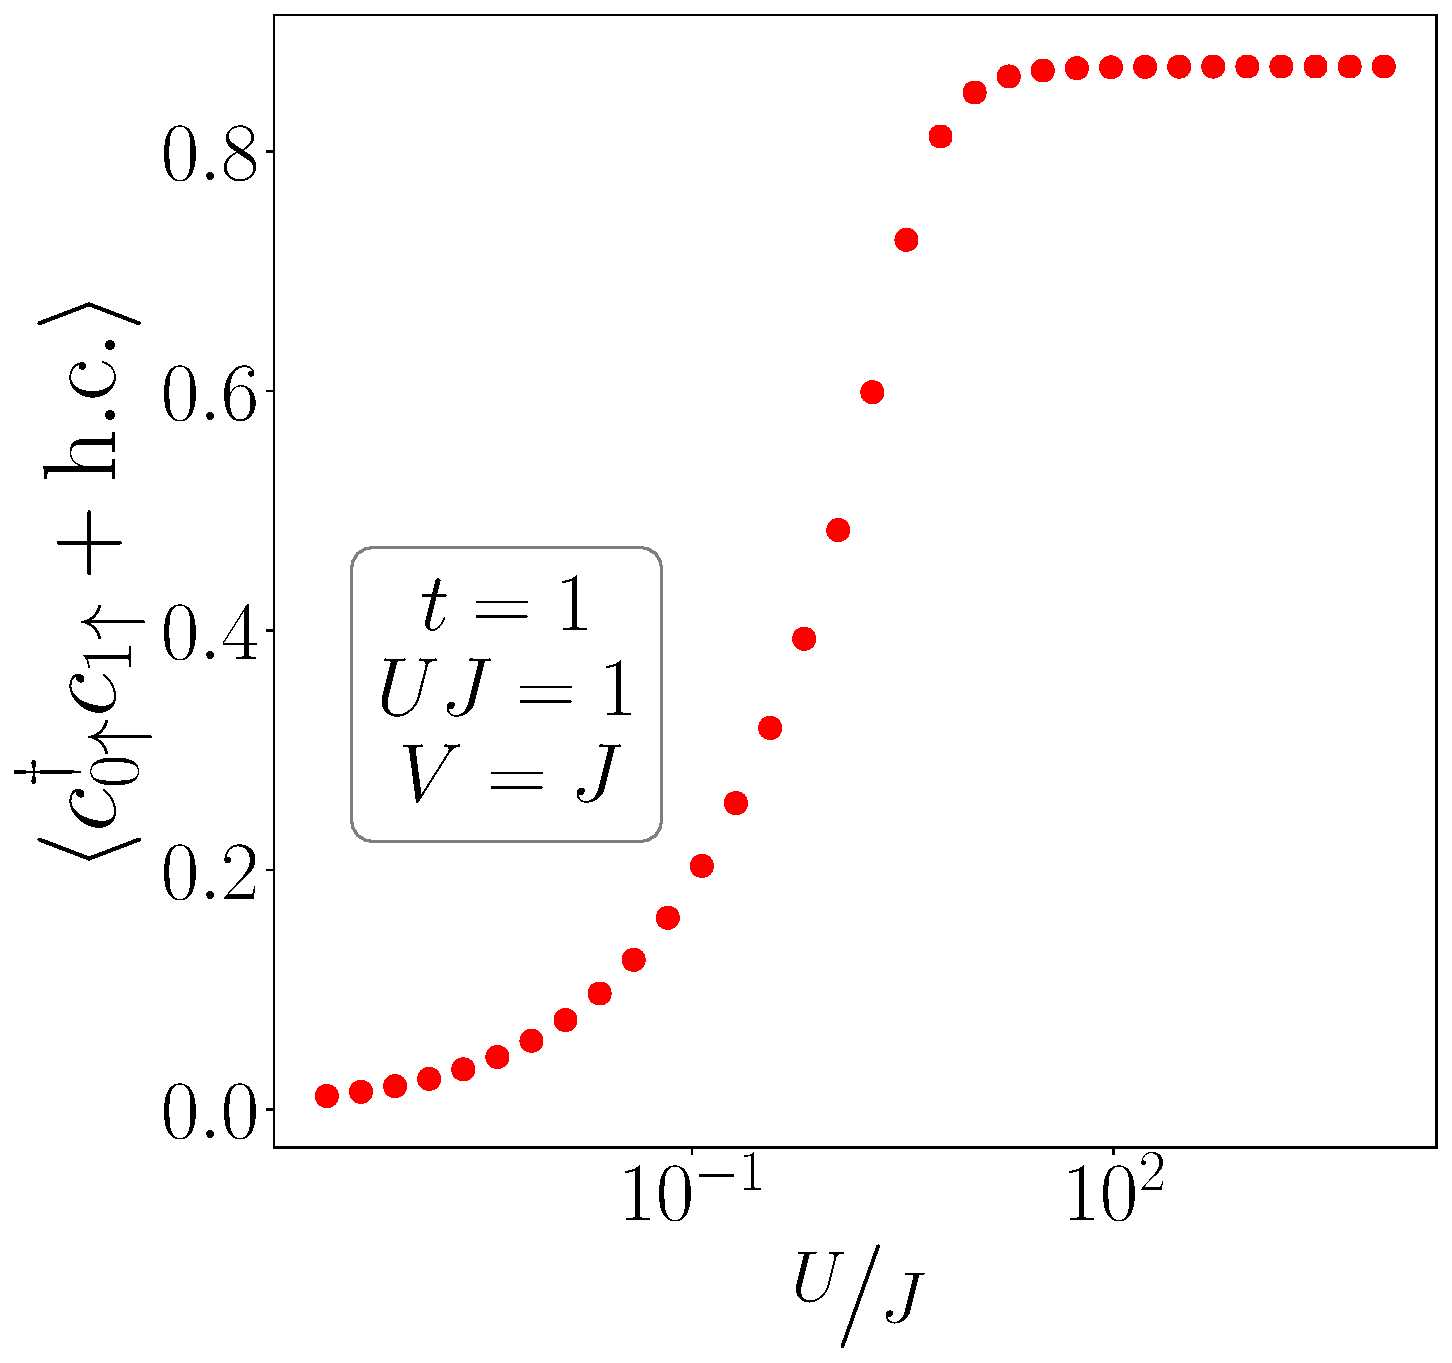
\includegraphics[width=0.32\textwidth]{../figures/r1p-t=1.000,J=1_over_U,V=J,N=6,U=0.016,91.116,32.pdf}
	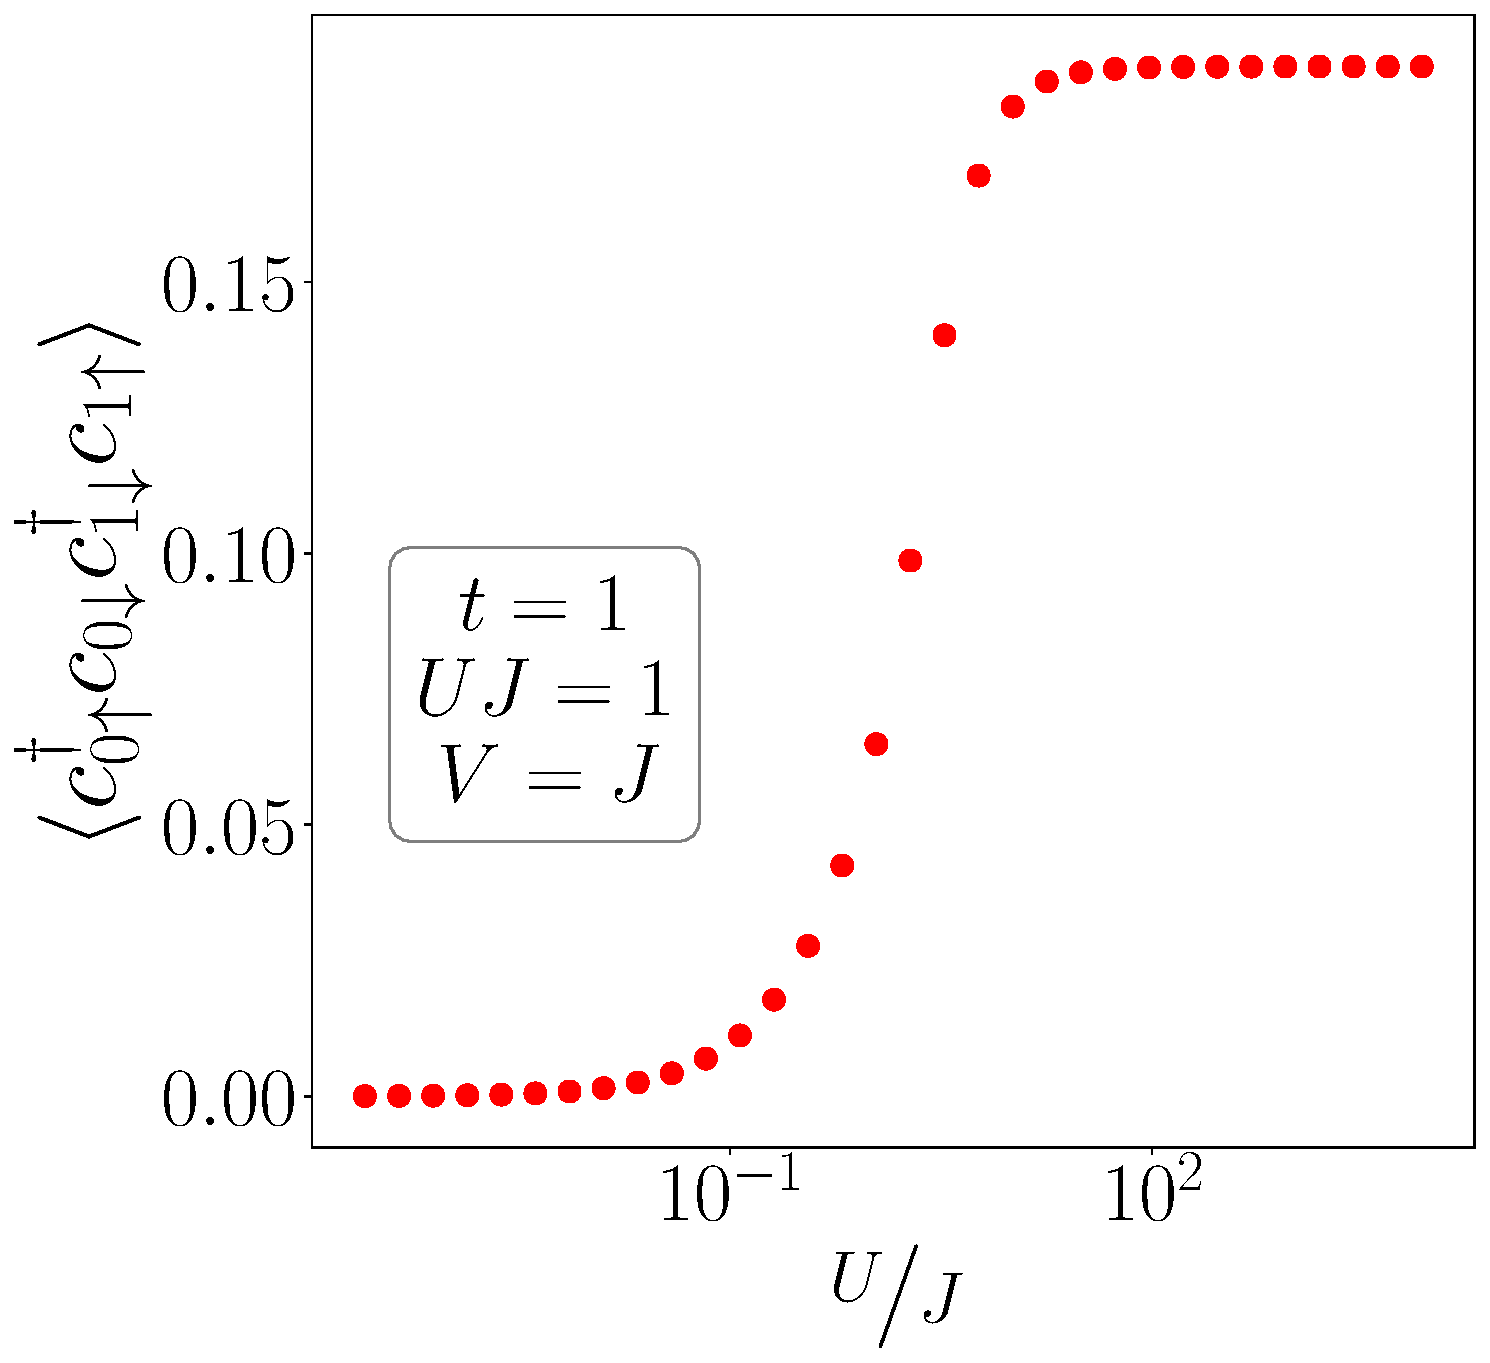
\includegraphics[width=0.32\textwidth]{../figures/r-od-t=1.000,J=1_over_U,V=J,N=6,U=0.016,91.116,32.pdf}
	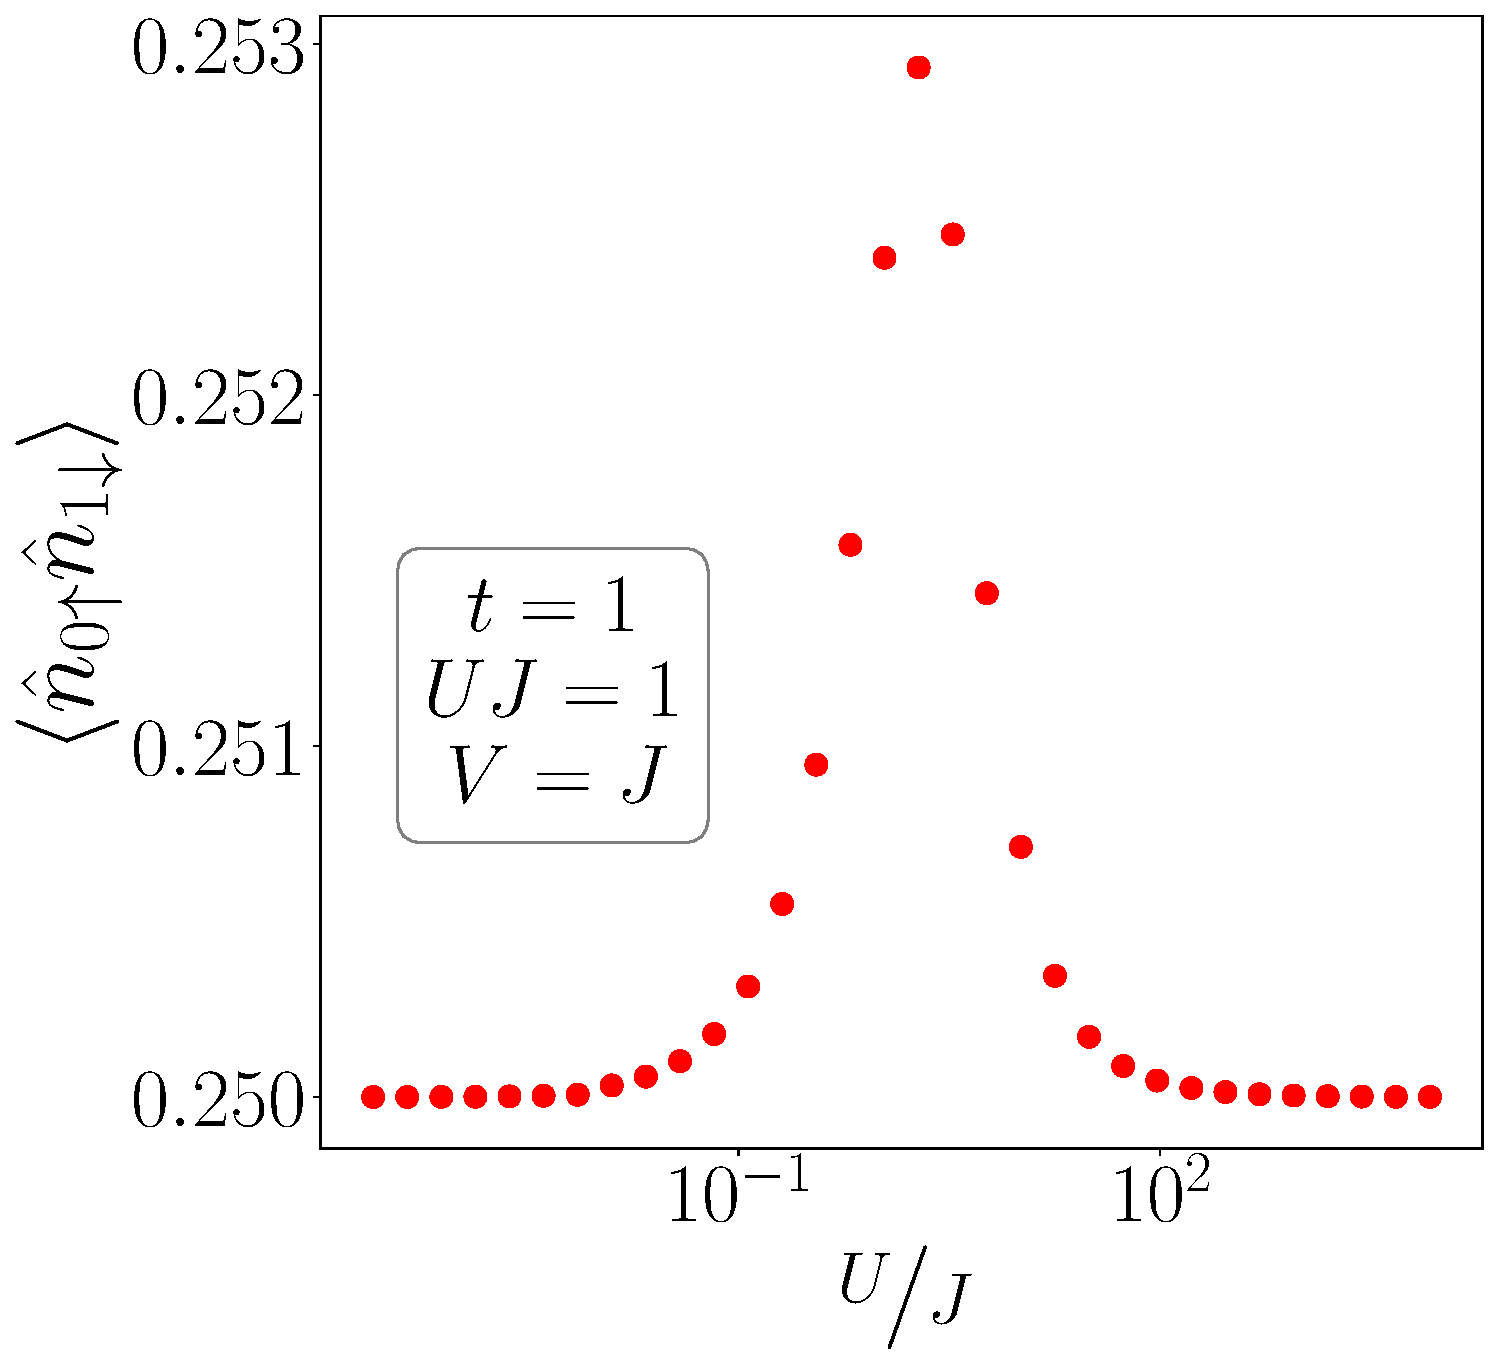
\includegraphics[width=0.32\textwidth]{../figures/r-opp-t=1.000,J=1_over_U,V=J,N=4,U=0.016,91.116,32.pdf}

	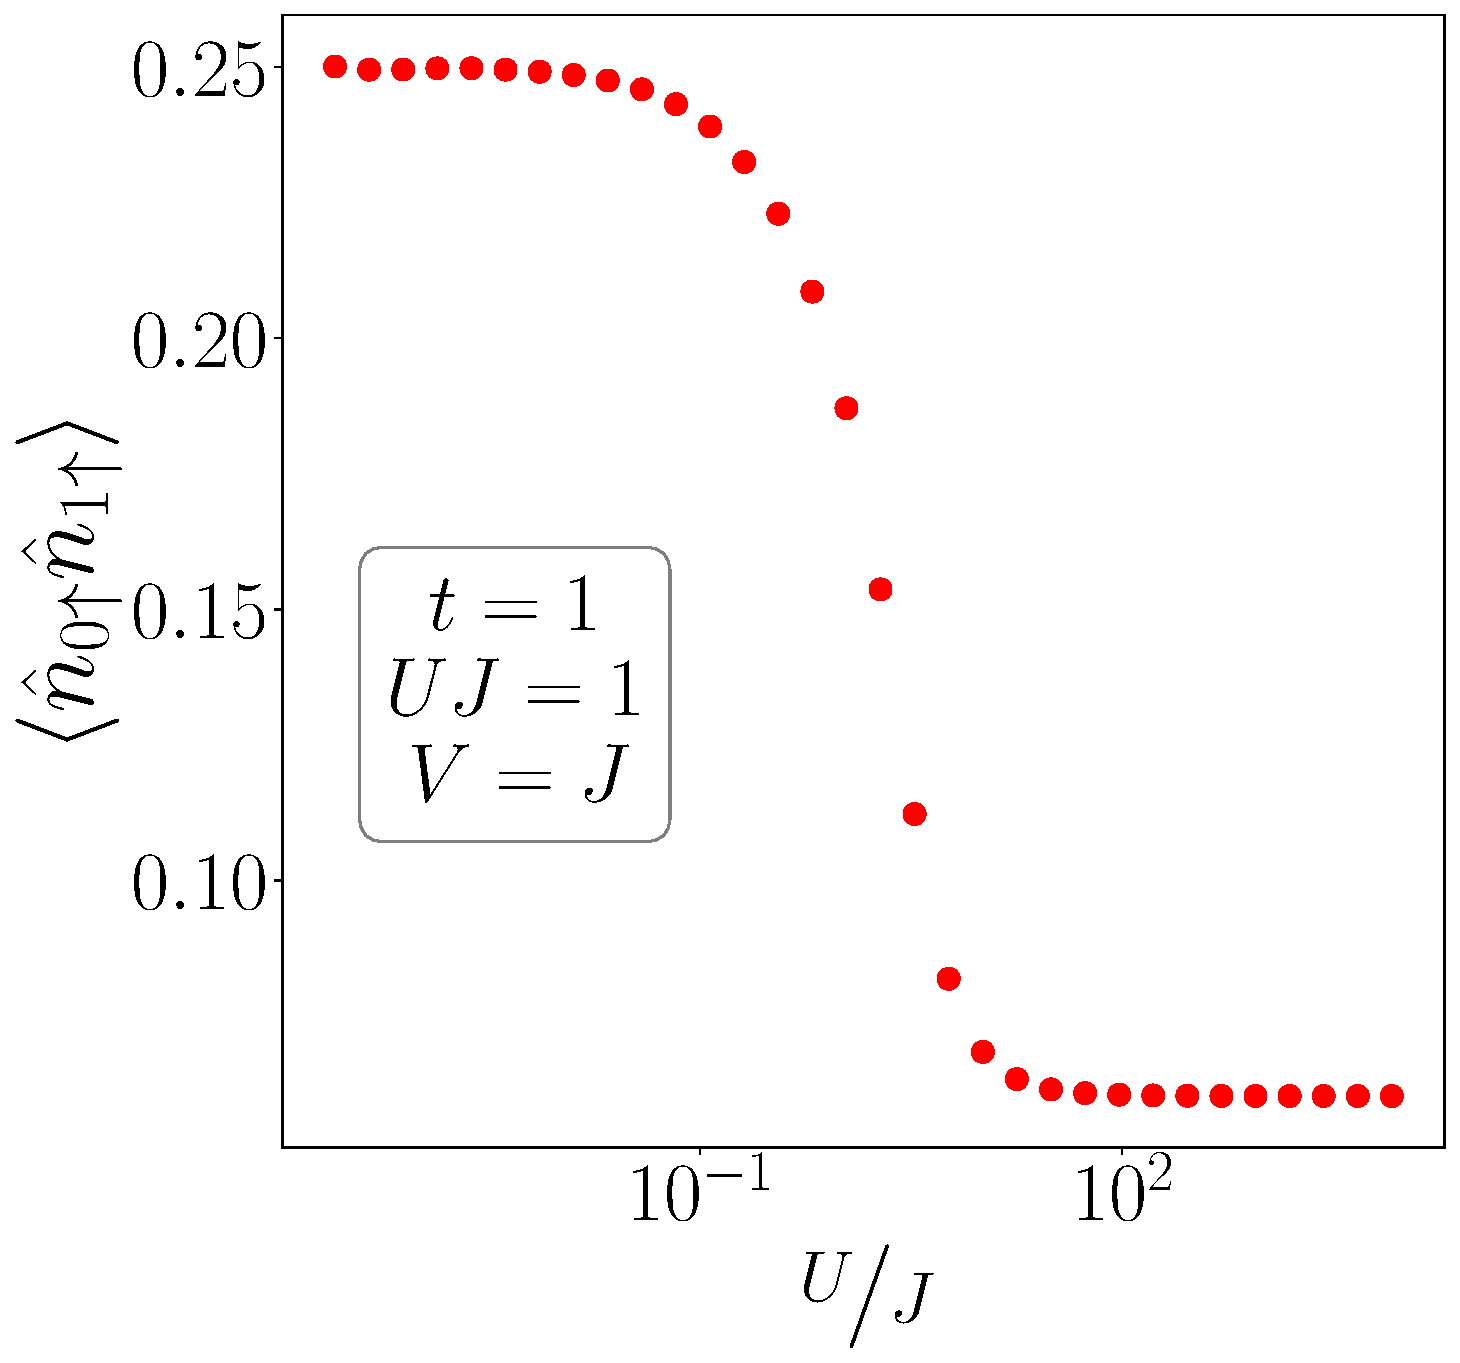
\includegraphics[width=0.3\textwidth]{../figures/r-par-t=1.000,J=1_over_U,V=J,N=6,U=0.016,91.116,32.pdf}
	\includegraphics[width=0.3\textwidth]{../figures/r-ising-t=1.000,J=1_over_U,V=J,N=6,U=0.016,91.116,32.pdf}
	\includegraphics[width=0.3\textwidth]{../figures/r-charge-t=1.000,J=1_over_U,V=J,N=6,U=0.016,91.116,32.pdf}
\end{center}

\subsection*{Real-space correlations as function of distance}
\begin{center}
	\includegraphics[width=0.45\textwidth]{../figures/corr-di-min-t=1.000,J=1_over_U,V=J,N=6,U=0.016,91.116,32.pdf}
	\includegraphics[width=0.45\textwidth]{../figures/corr-di-max-t=1.000,J=1_over_U,V=J,N=6,U=0.016,91.116,32.pdf}

	\includegraphics[width=0.45\textwidth]{../figures/corr-all-t=1.000,J=1_over_U,V=J,N=6,U=0.016,91.116,32.pdf}
	\includegraphics[width=0.45\textwidth]{../figures/I-all-t=1.000,J=1_over_U,V=J,N=6,U=0.016,91.116,32.pdf}
\end{center}

\subsection*{Impurity spectral function}
\begin{center}
	\includegraphics[width=0.32\textwidth]{../figures/spec-func-gen-siam-U_by_J=0.100.pdf}
	\includegraphics[width=0.32\textwidth]{../figures/spec-func-gen-siam-U_by_J=9.000.pdf}
	\includegraphics[width=0.32\textwidth]{../figures/spec-func-gen-siam-U_by_J=16.000.pdf}
	\includegraphics[width=0.32\textwidth]{../figures/spec-func-gen-siam-U_by_J=20.250.pdf}
	\includegraphics[width=0.32\textwidth]{../figures/spec-func-gen-siam-U_by_J=36.000.pdf}
\end{center}

\section{Calculating the \(T=0\) Wilson ratio from low energy excitations}
The total system now consists of two decoupled parts - the singlet composed of the impurity and the zeroth site, and the remaining lattice composed of N-1 sites with a tight-binding dispersion and a local interaction at the 1-th site. The effective Hamiltonian for the remaining lattice is
\begin{equation}\begin{aligned}
	\sum_{i=1\atop{\sigma}}^\infty t\left(c^\dagger_{i\sigma}c_{i+1 \sigma} + c^\dagger_{i+1 \sigma}c_{i\sigma}\right) + u \hat n_{1 \uparrow} \hat n_{1 \downarrow}
\end{aligned}\end{equation}
We have rewritten the holon term in terms of the spin and doublon operators.
\begin{figure}[htpb]
	\centering
	\includegraphics[width=0.7\textwidth]{../figures/lattice_eff.png}
	\caption{\textit{Left}: The nearest-neighbor hopping described by the effective Hamiltonian. The red circle is the impurity. The black cloud at the center demarcates the collection of electrons at the origin of the lattice (which couple to the impurity). The green circles represent lattice sites that are nearest to the origin. The blue circles represent next-nearest sites. \textit{Right}: After treating the hopping between origin and its nearest neighbors as perturbation, we get a system consisting of two decoupled parts: one part is the impurity+cloud singlet, the other part is the rest of the lattice sites. The effect of the hopping between the origin and the green sites is a repulsion term on the green sites.}
\end{figure}
We will now invoke the mean-field approximation in simplifying this term. We will be dealing with thermodynamic quantities soon, so the operators will be replaced by their thermodynamic values, that is, the values that minimize the free energy functional.
\begin{equation}\begin{aligned}
	\hat n_{1 \uparrow} \hat n_{1 \downarrow} \to \langle \hat n_{1 \uparrow} \hat n_{1 \downarrow}\rangle = \langle  \delta n_{1 \uparrow} \delta n_{1 \downarrow}\rangle + \langle  n_{1 \uparrow}\rangle\langle  n_{1 \downarrow}\rangle
\end{aligned}\end{equation}
where \(\delta n_{1\sigma} \equiv n_{1 \sigma} - \langle  n_{1\sigma} \rangle\) is the fluctuation of the particle number above the ground state. The mean-field approximation then involves dropping the first term which is a quadratic fluctuation - since we are interested in values of quantities at \( T \to 0\), this quadratic fluctuation is very small. The interaction we are left with is 
\begin{equation}\begin{aligned}
	u\langle  n_{1 \uparrow}\rangle\langle  n_{1 \downarrow}\rangle = \sum_{kq\sigma}f_{kq}\langle  n_{k \sigma}\rangle\langle  n_{q \overline\sigma}\rangle
\end{aligned}\end{equation}
This interaction converts the problem to that of a Landau Fermi liquid, with the quasiparticle energy functional being given by
\begin{equation}\begin{aligned}
	\epsilon_{k\sigma} = \epsilon_k + \sum_{q}f_{kq}\left<\hat n_{q \overline\sigma}\right>
\end{aligned}\end{equation}
From the form of the quasiparticle energy functional, we can see that there is no spin-parallel term, so we can write
\begin{equation}\begin{aligned}
	\label{rel_landau}
	f_{kk^\prime\sigma\sigma} = 0,  f_{kk^\prime\sigma\overline\sigma} = f_{kk^\prime}
\end{aligned}\end{equation}
We will now use this Fermi liquid form to extract the Wilson ratio. We will make use of the following definitions/results:
\begin{gather}
	dn_{k\sigma} = \frac{\partial{n}}{\partial{\epsilon_{k\sigma}}}\left( d\epsilon_{k\sigma} - d\mu \right) ~ ~ \left[\text{follows from differentiating FD distribution}\right] \\
	C_V = \frac{\:\mathrm{d}\epsilon}{\:\mathrm{d}T}, ~ ~ \chi^{s,c} = \frac{\:\mathrm{d}}{\:\mathrm{d}(B, \mu)}\left(n_\uparrow \mp n_\downarrow\right), ~ ~ 2f_0^{s,a} = \sum_k\left(f_{kk^\prime \uparrow \uparrow} \pm f_{kk^\prime \uparrow \downarrow}\right), ~ ~ F_0^{s,a} = \rho(0) f_0^{s,a}
\end{gather}
\subsection{Low-\(T\) Specific heat}
\begin{equation}\begin{aligned}
	C &= \frac{\:\mathrm{d}}{\:\mathrm{d}T}\sum_{k\sigma}\epsilon_{k\sigma}n_{k\sigma} \\
	    &\approx \sum_{k\sigma}\epsilon^0_{k\sigma} \frac{\:\mathrm{d}n_{k\sigma}}{\:\mathrm{d}T} && \left[\text{no quasiparticles at ground state}\right] \\
	    &\approx \sum_{k\sigma}\epsilon^0_{k\sigma} \frac{\:\mathrm{d}n_{k\sigma}}{\:\mathrm{d}T} && \left[\text{same expression as Fermi gas but with modified distribution function}\right] \\
	    &= \rho(0) T
\end{aligned}\end{equation}
where \(\rho\) is the total quasiparticle DOS with contributions from conduction bath and impurity.
\begin{equation}\begin{aligned}
	\rho \sim \text{Im }\text{Trace}\left[G\right] = \text{Im}\sum_{d\sigma}G_{dd}^\sigma + \text{Im}\sum_{k\sigma}G_{kk}^\sigma = \rho_0 + \rho_\text{imp}
\end{aligned}\end{equation}
which gives
\begin{equation}\begin{aligned}
	C_{imp} \equiv C - C_0 = \rho_{imp}(0)T
\end{aligned}\end{equation}

\subsection{Low-\(T\) Charge Susceptibility}
\begin{equation}\begin{aligned}
	\chi^c &= \frac{\:\mathrm{d}N}{\:\mathrm{d}\mu}\\
\end{aligned}\end{equation}
Due to change in chemical potential, \(\delta\epsilon_{k\sigma}\) is isotropic and SU(2)-symmetric. Hence
\begin{equation}\begin{aligned}
	d\epsilon_{k\sigma} &= \sum_{k^\prime\sigma^\prime}f_{kk^\prime\sigma\sigma^\prime}d n_{k^\prime\sigma^\prime}\\
			    &= d n\sum_{k^\prime}\left(f_{kk^\prime\uparrow \uparrow} + f_{kk^\prime \uparrow \downarrow}\right) && \left[dn = dn_{k^\prime \uparrow} = dn_{k \downarrow}\right] \\
			    &= 2dn f_0^s
\end{aligned}\end{equation}
Therefore,
\begin{equation}\begin{aligned}
	dN &= \sum_{k\sigma}dn_{k\sigma} = \sum_{k\sigma}\frac{\partial{n}}{\partial{\epsilon_{k\sigma}}}\left( d\epsilon_{k\sigma} - d\mu \right) = \sum_{k\sigma}-\frac{1}{2}\rho\left(2dn f_0^s - d\mu \right) = -\rho(0) d N f_0^s + d\mu \rho(0) \\
	   &\approx d\mu \rho(0) - \rho(0) f_0^s d\mu \rho(0) \left[\text{substitute \(dN\) back into itself}\right] \\
	\implies \frac{\:\mathrm{d}N}{\:\mathrm{d}\mu} &= \rho(0)\left( 1 - \rho(0)f_0^s \right) \implies \chi^c_{imp} = \rho(0)_{imp} - \rho(0)f_0^s \\
\end{aligned}\end{equation}
At an intermediate state, we substituted \(dN\) back into itself and kept only the leading order term. This is justified because \(f_{kk^\prime}\) goes as \(\frac{1}{N J}\). At the fixed point and for a thermodynamically large system, both \(J\) and \(N\) are very large, so keeping only the leading order suffices.

From a previous calculation, we know that the charge susceptibility at \(T=0\) is zero (eq.~\eqref{zero_chi_charge}), so we can write down the following relation:
\begin{equation}\begin{aligned}
	\label{fp_constraint}
	f_0^s = \frac{\rho(0)_{imp}}{\rho(0)}
\end{aligned}\end{equation}

\subsection{Low-\(T\) Spin Susceptibility}
\begin{equation}\begin{aligned}
	\chi^s &= \frac{\:\mathrm{d}m}{\:\mathrm{d}\mu}\\
\end{aligned}\end{equation}
Due to change in magnetic field, change in \(\epsilon_{k\sigma}\) should be isotropic and SU(2)-\text{anti}symmetric. Hence
\begin{equation}\begin{aligned}
	d\epsilon_{k\sigma} &= -\frac{1}{2}dB \sigma + \sum_{k^\prime\sigma^\prime}f_{kk^\prime\sigma\sigma^\prime}d n_{k^\prime\sigma^\prime}\\
			    &= -\frac{1}{2}dB \sigma + d n_{\sigma}\sum_{k^\prime}\left(f_{kk^\prime\uparrow \uparrow} - f_{kk^\prime \uparrow \downarrow}\right) && \left[dn_{k^\prime \uparrow} = -dn_{k \downarrow}\right] \\
			    &= -\frac{1}{2}dB \sigma + 2dn_\sigma f_0^a
\end{aligned}\end{equation}
Since the total number remains constant, \(\mu=0\). Therefore,
\begin{equation}\begin{aligned}
	dm &= \sum_{k}\left(dn_{k \uparrow} - dn_{k \downarrow}\right) = -\frac{1}{2}\sum_{k}\rho\left( d\epsilon_{k \uparrow} - d\epsilon_{k \downarrow} \right) = -\frac{1}{2}\sum_{k}\rho\left(-dB + 2f_0^a \left(dn_{k \uparrow} - dn_{k \downarrow}\right)\right) \\
	   &= dB\rho(0) - dm \rho(0)f_0^a \approx dB\rho(0) - \rho(0)f_0^aB\rho(0) ~ \left[\text{substitute \(dm\) back into itself}\right] \\
	\implies \frac{\:\mathrm{d}m}{\:\mathrm{d}B} &= \rho(0)\left( 1 - \rho(0)f_0^a \right) \implies \chi^s_{imp} = \rho(0)_{imp} - \rho(0)f_0^a \\
\end{aligned}\end{equation}

\subsection{Wilson ratio}
The Wilson ratio for the impurity is defined as
\begin{equation}\begin{aligned}
	R = \frac{\chi^s_{imp}}{\frac{C_{imp}}{T}}
\end{aligned}\end{equation}
From eq.~\eqref{rel_landau}, we have \(f_0^s = -f_0^a\), which, when combined with eq.~\eqref{fp_constraint}, gives
\begin{equation}\begin{aligned}
	\chi^s_{imp} &= 2\rho(0)_{imp}
\end{aligned}\end{equation}
The Wilson ratio becomes
\begin{equation}\begin{aligned}
	R = \frac{2\rho(0)_{imp}}{\rho(0)_{imp}} = 2
\end{aligned}\end{equation}

\section{Luttinger's and Friedel's sum rules}
The subsequent discussions are for the first quadrant where \(U^* = 0\) and \(J^* > K^*\). At high temperatures, we see that the impurity susceptibility attains the value of
\begin{equation}\begin{aligned}
	\frac{1}{8k_B T}
\end{aligned}\end{equation}
which implies that the impurity behaves as a free orbital in this limit, having no coupling with the bath. We can write down the following effective Hamiltonian for such a limit:
\begin{equation}\begin{aligned}
	\mathcal{H}_\text{high-T} = \tilde \epsilon_d \hat n_d + \sum_{k\sigma} \epsilon_k\hat n_{k\sigma}
\end{aligned}\end{equation}
Since the impurity is decoupled from the bath, we can immediately write down the Hamiltonian just for the impurity:
\begin{equation}\begin{aligned}
	\mathcal{H}_\text{high-T, imp} = \tilde \epsilon_d \hat n_d
\end{aligned}\end{equation}

We consider the resonant-level model:
\begin{equation}\begin{aligned}
	\mathcal{H}_\text{res} = \sum_{k\sigma}\epsilon_k \hat n_{k\sigma} + \epsilon_d n_d + \sum_{k\sigma}\left(V_k c^\dagger_{k\sigma} c_{d\sigma} + \text{h.c.}\right)
\end{aligned}\end{equation}
The total Green's function is 
\begin{equation}\begin{aligned}
	G(z) = \frac{1}{z - \mathcal{H}_\text{res}}
\end{aligned}\end{equation}
The impurity diagonal Green's function is
\begin{equation}\begin{aligned}
	G_{dd}(z) &= \frac{1}{z - \epsilon_d - \Sigma_d(z)}, &&	G_d(z) = G_{dd}\ket{d}\bra{d}
\end{aligned}\end{equation}
where \(\Sigma_d(z)\) is in general complex and is zero at the free orbital fixed point. The conduction electron Green's function is 
\begin{equation}\begin{aligned}
	&G_{kk}(z) = G_k^0(z) + \left[G_k^0(z)V_k\right]^2 G_{dd}(z), & G_c(z) \equiv \sum_k \ket{k}\bra{k}G_{kk}(z), && G_{c0}(z) \equiv \sum_k G_{kk}^0(z)\ket{k}\bra{k}
\end{aligned}\end{equation}
The total Green's function can be written as
\begin{equation}\begin{aligned}
	G(z) &= \left(\sum_{k}\ket{k}\bra{k} + \ket{d}\bra{d}\right) G \left(\sum_{k}\ket{k}\bra{k} + \ket{d}\bra{d}\right)\\
	     &= \sum_{k} \ket{k}\bra{k}G_{kk}(z) + G_{dd}(z)\ket{d}\bra{d} + \text{off-diagonal terms}\\
	     &= G_c(z) + G_{d}(z) + \text{off-diagonal terms}
\end{aligned}\end{equation}
The total number of electrons is given by
\begin{equation}\begin{aligned}
	N &= \oint \frac{dz}{2\pi i}n_F(z) \text{Tr}\left[G(z) \right]\\
	  &= \oint \frac{dz}{2\pi i}n_F(z) \text{Tr}\left[G_{d}(z) + G_c(z)\right]
\end{aligned}\end{equation}
The contour \(\Gamma\) counts all the singularities of \(\text{Tr} G(z)\), and thus encloses only the real axis of the complex plane (since \(G(z)\) comes from a Hermitian matrix \(\mathcal{H}_\text{res}\), all its singularities are real).
At this point, we can use an identity:
\begin{equation}\begin{aligned}
	\text{Tr}\left[G_{d}(z)\right] &= \text{Tr}\left[ \frac{\ket{d}\bra{d}}{z - \epsilon_d - \Sigma_d(z)}\right] = \text{Tr}\left[ \frac{\ket{d}\bra{d}}{z - \epsilon_d - \Sigma_d(z)}\frac{\partial{\left(z - \epsilon_d\right)}}{\partial{z}} \right] = \text{Tr}\left[ \ket{d}\bra{d}G_{dd}\frac{\partial{\left\{G_{dd}^{-1}(z) + \Sigma_d(z)\right\}}}{\partial{z}} \right]\\
				       &= \text{Tr}\left[ G_{d}(z)\frac{\partial{G_{d}^{-1}(z)}}{\partial{z}} \right] + \text{Tr}\left[ G_{d}(z)\frac{\partial{\Sigma_d(z)}}{\partial{z}} \right] = \frac{\partial{}}{\partial{z}}\left[\ln \text{Det}G_{d}^{-1}(z)\right] + \text{Tr}\left[ G_{d}(z)\frac{\partial{\Sigma_d(z)}}{\partial{z}} \right]\\
\end{aligned}\end{equation}
In the last step, we converted the trace to a determinant using
\begin{equation}\begin{aligned}
	\text{Tr}\left[A \frac{\partial{A^{-1}}}{\partial{z}}\right] = \frac{\partial{}}{\partial{z}}\text{Tr}\ln A^{-1} =\frac{\partial{}}{\partial{z}}\sum_i \ln \lambda_i = \frac{\partial{}}{\partial{z}}\ln \prod_i \lambda_i = \frac{\partial{}}{\partial{z}}\ln \text{Det}A^{-1}
\end{aligned}\end{equation}
where \(\lambda_i\) are the eigenvalues of \(A^{-1}\). Substituting \(\text{Tr}\left[G_d(z)\right] \) into the total number of particles gives
\begin{equation}\begin{aligned}
	N  &= \oint \frac{dz}{2\pi i}n_F(z) \left[\frac{\partial{}}{\partial{z}} \ln \text{Det} \left\{G^{-1}_d(z)\right\} + \text{Tr} \left( G_d(z) \frac{\partial{}}{\partial{z}}\Sigma_d(z) \right) + \text{Tr}G_c(z)\right]
\end{aligned}\end{equation}
The conduction electron part can also be simplified:
\begin{equation}\begin{aligned}
	\text{Tr}G_c(z) &= \text{Tr}\left[G_{c0}(z) + \sum_k \left\{G_k^0(z)V_k\right\}^2 G_{dd}(z)\ket{k}\bra{k}\right] =\text{Tr}\left[G_{c0}(z)\right] + \sum_k\left[G_k^0(z)V_k\right]^2 G_{dd}(z)\\
\end{aligned}\end{equation}
Since \(G_{c0}^{-1}(z) = z - \sum_k \epsilon_k \hat n_k\), we can write \(\text{Tr}\left[G_{c0}(z)\right] = \text{Tr}\left[G_{c0}(z) \frac{\partial{}}{\partial{z}}G_{c0}^{-1}\right]\) and hence
\begin{equation}\begin{aligned}
	\text{Tr}G_c(z) &=\frac{\partial{}}{\partial{z}}\left[\ln \text{Det}G_{c0}^{-1}(z)\right] + \sum_k\left[G_k^0(z)V_k\right]^2 G_{dd}(z)
\end{aligned}\end{equation}
Updating the total particles with this leads to
\begin{equation}\begin{aligned}
	N  = \oint \frac{dz}{2\pi i}n_F(z) \left[\frac{\partial{}}{\partial{z}} \ln \text{Det} \left\{G^{-1}_d(z)\right\} + \frac{\partial{}}{\partial{z}} \ln \text{Det} \left\{G^{-1}_{c0}(z)\right\} + \text{Tr} \left( G_d(z) \frac{\partial{}}{\partial{z}}\Sigma_d(z) \right) + \sum_k\left( V_k G_k^0 \right)^2 G_{dd}(z)\right]
\end{aligned}\end{equation}
For the resonant-level model, we have
\begin{equation}\begin{aligned}
	\Sigma_d = \sum_k V^2_k G^0_k = \sum_k \frac{V_k^2}{z - \epsilon_k}
\end{aligned}\end{equation}
such that
\begin{equation}\begin{aligned}
	\text{Tr} \left( G_d(z) \frac{\partial{}}{\partial{z}}\Sigma_d(z) \right) = -G_{dd}(z) \sum_k \left( V_k G_k^0 \right)^2
\end{aligned}\end{equation}
which allows us to write
\begin{equation}\begin{aligned}
	N  = \oint \frac{dz}{2\pi i}n_F(z) \left[\frac{\partial{}}{\partial{z}} \ln \text{Det} \left\{G^{-1}_d(z)\right\} + \frac{\partial{}}{\partial{z}} \ln \text{Det} \left\{G^{-1}_{c0}(z)\right\} \right]
\end{aligned}\end{equation}
At \(T=0\), \(n_F\) is defined as 1 below the FS, \(\frac{1}{2}\) at the FS and 0 above it.
\begin{equation}\begin{aligned}
	N  = \left[\oint_{\Gamma_<} + \frac{1}{2}\oint_{\Gamma_0}\right]\frac{dz}{2\pi i}\left[\frac{\partial{}}{\partial{z}} \ln \text{Det} \left\{G^{-1}_d(z)\right\} + \frac{\partial{}}{\partial{z}} \ln \text{Det} \left\{G^{-1}_{c0}(z)\right\} \right]
\end{aligned}\end{equation}
Following Seki and Yunoki, we can define a winding number for a Green's function \(G(z)\):
\begin{equation}\begin{aligned}
	n_{\text{Det} G^{-1}}(C) = \oint_{C} \frac{dz}{2\pi i} \frac{\partial{\ln\text{Det }G^{-1}(z)}}{\partial{z}} = \oint_{\text{Det} G^{-1}(C)} \frac{\mathrm{d}\; \text{Det }G^{-1}}{\text{Det }G^{-1}}
\end{aligned}\end{equation}
Since \(n_{\text{Det } G^{-1}(C)}\) counts the number of times the curve \(\text{Det } G^{-1}(C)\) winds around the origin, it is integer-valued and topological. Seki and Yunoki also show that the this number is given by
\begin{equation}\begin{aligned}
n_{\text{Det }G^{-1}(C)} = P_{\text{Det }G}(C) - Z_{\text{Det }G}(C)
\end{aligned}\end{equation}
where \(P_{f(z)}(C)\) is the number of poles of \(f(z)\) enclosed by the contour \(C\), and \(Z\) is the corresponding number of zeros. The total number of particles in the resonant level model can thus be written as
\begin{equation}\begin{aligned}
	N = P_{\text{Det }G_d}(\Gamma_<) - Z_{\text{Det }G_d}(\Gamma_<) + \frac{1}{2}\left[P_{\text{Det }G_d}(\Gamma_0) - Z_{\text{Det }G_d}(\Gamma_0)\right] + P_{\text{Det }G_{c0}}(\Gamma_<) - Z_{\text{Det }G_{c0}}(\Gamma_<) \\
	+ \frac{1}{2}\left[P_{\text{Det }G_{c0}}(\Gamma_0) - Z_{\text{Det }G_{c0}}(\Gamma_0)\right]
\end{aligned}\end{equation}
The average number of particles can thus be expressed purely in terms of the number of poles and zeros of the impurity and the conduction electron Green's functions. As shown by Seki and Yunoki, the second line gives the Luttinger volume \(V_L\):
\begin{equation}\begin{aligned}
	\label{total_lutt}
	N = P_{\text{Det }G_d}(\Gamma_<) - Z_{\text{Det }G_d}(\Gamma_<) + \frac{1}{2}\left[P_{\text{Det }G_d}(\Gamma_0) - Z_{\text{Det }G_d}(\Gamma_0)\right] + V_L
\end{aligned}\end{equation}
If we start from a non-interacting model (\(V_k = 0\)), we can write
\begin{equation}\begin{aligned}
	N = \mathcal{N}^0_{imp} + V_L^0
\end{aligned}\end{equation}
where \(\mathcal{N}^0_{imp}\) is simply the number of singularities of \(G_d\) on the real axis, for the non-interacting case. We now turn up the interaction \(V_k\), keeping the total number of particles conserved at \(N\). With a non-zero \(V_k\), the impurity self-energy can be written (assuming a constant density of states) as
\begin{equation}\begin{aligned}
	\Sigma_d(z) = \Sigma_d^\text{real}(z) - i \Delta
\end{aligned}\end{equation}
so that the impurity Greens function becomes
\begin{equation}\begin{aligned}
	G_d(z) = \frac{1}{z - \epsilon_d - \Sigma_d^\text{real}(z) + i \Delta}
\end{aligned}\end{equation}
We can see that the presence of an imaginary part lifts the pole of \(G_d(z)\) off the real axis, and since the contour \(\Gamma_0\) encloses only the real axis, this will count as a loss in the number of poles of \(G_d(z)\). Also, if we specialize to the case where the renormalized impurity site energy \(\epsilon_d^* = \epsilon_d + \Sigma_d^\text{real} = 0\), this loss will happen at the Fermi surface, and will hence be multiplied by a factor of half. We can therefore write
\begin{equation}\begin{aligned}
	N &= \mathcal{N}_{imp} + V_L = \mathcal{N}^0_{imp} - \frac{1}{2} + V_L \implies V_L &= V_L^0 + \frac{1}{2}
\end{aligned}\end{equation}
If we take into account the spin-degeneracy and redefine \(V_L\) to mean the Luttinger volume for both momentum and spin degrees of freedom, we get
\begin{equation}\begin{aligned}
	\label{luttinger_change}
	V_L = V_L^0 + 1
\end{aligned}\end{equation}
\begin{figure}[htpb]
	\centering
	\includegraphics[scale=0.2]{../figures/luttinger_top_change.png}
\end{figure}
This is a specific case of the more general result for Kondo lattices obtained by Oshikawa using flux-insertion arguments in \cite{oshikawa2000topological}.
One can now ask what happens to this result once we also incorporate the spin-exchange interaction \(J \vec{S_d}\cdot\vec{s}\); we can expect that it will complicate the self-energy of the impurity. It cannot, however, preclude the loss of the real pole, nor can it create a new singularity - to do so would require the self-energy to diverge, and we are working with finite systems here. This suggests that the eq.~\eqref{luttinger_change} would still hold.

We have also not accounted for the RG flow from the local moment fixed point to the strong-coupling fixed point. The local moment fixed point is characterized by a decoupled quantum top:
\begin{equation}\begin{aligned}
	\mathcal{H}_\text{LM} = \epsilon_d \hat n_d + U \hat n_{d \uparrow} \hat n_{d \downarrow}
\end{aligned}\end{equation}
It can be shown that the single-particle Green's function for this effective Hamiltonian is similar to the one at the free-orbital fixed point. We will use the equation of motion technique to solve for the Green's function. The time-domain retarded Green's function is defined as
\begin{equation}\begin{aligned}
	G_{d\sigma}(t, t^\prime) = -i\theta(t-t^\prime) \left<\left\{ c_{d\sigma}(t), c^\dagger_{d\sigma}(t^\prime) \right\} \right>
\end{aligned}\end{equation}
Since the Hamiltonian is time-translation invariant, we can drop one of the instants:
\begin{equation}\begin{aligned}
	G_{d\sigma}(t, 0) = -i\theta(t) \left<\left\{ c_{d\sigma}(t), c^\dagger_{d\sigma}(0) \right\} \right>
\end{aligned}\end{equation}
The time derivative is
\begin{equation}\begin{aligned}
	\partial_t G_{d\sigma} &= -i \left[\partial_t \theta(t) \left<\left\{ c_{d\sigma}(t), c^\dagger_{d\sigma}(0) \right\} \right> + \theta(t) \partial_t \left<\left\{ c_{d\sigma}(t), c^\dagger_{d\sigma}(0) \right\} \right>\right] \\
			       &= -i \left[\delta(t) \left<\left\{ c_{d\sigma}(t), c^\dagger_{d\sigma}(0) \right\} \right> + \theta(t) \left<\left\{ \partial_t c_{d\sigma}(t), c^\dagger_{d\sigma}(0) \right\} \right>\right] = -i \delta(t) -i\theta(t) \left<\left\{ \partial_t c_{d\sigma}(t), c^\dagger_{d\sigma}(0) \right\} \right>
\end{aligned}\end{equation}
From the Heisenberg equations of motion, we get
\begin{equation}\begin{aligned}
	i \partial_t c_{d\sigma}(t) = \left[c_{d\sigma}(t), \mathcal{H}_{LM}(t)\right] = \left[\epsilon_d + U \hat n_{d\overline\sigma}(t)\right]c_{d\sigma}(t)
\end{aligned}\end{equation}
Substituting this into the time-derivative gives
\begin{equation}\begin{aligned}
	\partial_t G_{d\sigma} &= -i \delta(t) -i \theta(t) \left<\left\{ -i\left[\epsilon_d + U \hat n_{d\overline\sigma}(t)\right]c_{d\sigma}(t), c^\dagger_{d\sigma}(0) \right\} \right> = -i \delta(t) - i\epsilon_d G_{d\sigma} - U \theta(t) \left<\hat n_{d\overline\sigma}(t)\left\{c_{d\sigma}(t), c^\dagger_{d\sigma}(0) \right\} \right>\\
\end{aligned}\end{equation}
We define another Greens function
\begin{equation}\begin{aligned}
	G^\prime = -i \theta(t) \left<\hat n_{d\overline\sigma}(t)\left\{c_{d\sigma}(t), c^\dagger_{d\sigma}(0) \right\} \right>
\end{aligned}\end{equation}
which satisfies the equation of motion
\begin{equation}\begin{aligned}
	\partial_t G^\prime = -i \delta(t) -i\theta(t) \left<\left\{\partial_t \hat n_{d\overline\sigma}(t)c_{d\sigma}(t), c^\dagger_{d\sigma}(0) \right\} \right> -i\theta(t) \left<\left\{\hat n_{d\overline\sigma}(t)\partial_t c_{d\sigma}(t), c^\dagger_{d\sigma}(0) \right\} \right>
\end{aligned}\end{equation}
The second term vanishes because \(\left[\hat n_{d\overline\sigma}, \mathcal{H}_{LM}\right] = 0\) and hence \(\partial_t \hat n_{d\overline\sigma} = 0\). Also,
\begin{equation}\begin{aligned}
	\hat n_{d\overline\sigma}(t)\partial_t c_{d\sigma}(t) = -i\hat n_{d\overline\sigma}(t)\left[\epsilon_d + U \hat n_{d\overline\sigma}(t)\right]c_{d\sigma}(t) = -i\left[\epsilon_d + U\right]\hat n_{d\overline\sigma}(t)c_{d\sigma}(t)
\end{aligned}\end{equation}
Therefore,
\begin{equation}\begin{aligned}
	\partial_t G^\prime = -i \delta(t) \left< \hat n_{d\overline\sigma}(0)\right>- \left[\epsilon_d + U\right]\theta(t) \left<\left\{\hat n_{d\overline\sigma}(t)c_{d\sigma}(t), c^\dagger_{d\sigma}(0) \right\} \right> = -i \delta(t) -i \left( \epsilon_d + U \right) G^\prime
\end{aligned}\end{equation}
Changing all quantities to frequency-domain:
\begin{equation}\begin{aligned}
	G^\prime(t) &= \int_{-\infty}^\infty d\omega e^{-i\omega t} G^\prime(\omega)\\
	\partial_t G^\prime(t) &= -\int_{-\infty}^\infty d\omega i \omega e^{-i\omega t} G^\prime(\omega)\\
	\delta(t) &= \int_{-\infty}^\infty d\omega e^{-i\omega t}
\end{aligned}\end{equation}
Substituting these forms in the equation and comparing the coefficients of \(e^{i\omega t}\) gives
\begin{equation}\begin{aligned}
	 \omega G^\prime(\omega) =  \left< \hat n_{d\overline\sigma}(0)\right> + \left( \epsilon_d + U \right) G^\prime(\omega)\implies G^\prime(\omega) = \frac{\left< \hat n_{d\overline\sigma}(0)\right>}{\omega - \epsilon_d - U}
\end{aligned}\end{equation}
The equation of motion \(G_{d\sigma}\) can now be solved
\begin{equation}\begin{aligned}
	\partial_t G_{d\sigma}(t) &= -i \delta(t) - i\epsilon_d G_{d\sigma}(t) - iU G^\prime_{d\sigma}(t) \implies \omega G_{d\sigma}(\omega) = 1 + \epsilon_d G_{d\sigma}(\omega) + U\frac{\left< \hat n_{d\overline\sigma}(0)\right>}{\omega - \epsilon_d - U}\\
	\implies G_{d\sigma}(\omega) &= \frac{1}{\omega - \epsilon_d} + \frac{U\left< \hat n_{d\overline\sigma}(0)\right>}{\left( \omega - \epsilon_d \right) \left(\omega - \epsilon_d - U\right)}
\end{aligned}\end{equation}
For a particle-hole symmetric system, we can substitute \(\epsilon_d = -|\epsilon_d|\) and \(\epsilon_d + U = |\epsilon_d|\).
\begin{equation}\begin{aligned}
	G_{d\sigma}(\omega) &= \frac{1}{\omega + |\epsilon_d|} + \frac{U\left< \hat n_{d\overline\sigma}(0)\right>}{\left( \omega + |\epsilon_d| \right) \left(\omega - |\epsilon_d|\right)}
\end{aligned}\end{equation}
which reveals two poles at \(\pm |\epsilon_d|\), one above and one below the Fermi surface. Since the RHS of eq.~\eqref{total_lutt} counts the number of poles on or below the FS, we will still count one pole for \(G_{d\sigma}\). Thus, this Green's function is topological similar to the free-orbital one at \(T=0\).

The scattering phase shift suffered by the conduction electrons at the Fermi surface, off the impurity, can be calculated from the impurity occupancy, using the Friedel sum rule. From the ground state wavefunction, we can calculate the average number of particles on the impurity:
\begin{equation}\begin{aligned}
	\left<n_d \right> = \bra{\Psi}_1\sum_\sigma \hat n_{d\sigma} \ket{\Psi}_1
\end{aligned}\end{equation}
\(\ket{\Psi}_1\) is the lower energy state in eq.~\eqref{gstate}. Performing the inner product gives
\begin{equation}\begin{aligned}
	\left<n_d \right> = \left( c_s^- \right)^2 + \left( c_c^- \right)^2 = 1
\end{aligned}\end{equation}
The phase shift is thus
\begin{equation}\begin{aligned}
	\frac{1}{\pi}\sum_\sigma \delta_\sigma(0) = \left<n_d \right> \implies \delta_\sigma(0) = \frac{\pi}{2}
\end{aligned}\end{equation}
There we used \(\delta_\uparrow = \delta_\downarrow\) because the model is SU(2)-symmetric. This line of arguments was first presented for the Kondo model in \cite{martin1982fermi}.

The change in Luttinger's number also allows us to calculate the Wilson ratio of the system, from eq.~\eqref{wilson_luttinger}.
\begin{equation}\begin{aligned}
	R = 1 + \sin^2 \left( \frac{\pi}{2}\Delta N_L \right) = 1 + \sin^2 \frac{\pi}{2} = 2
\end{aligned}\end{equation}
\section{Reverse RG analysis}\label{rev_rg}
The goal here is to chart the journey starting from the IR fixed point towards the UV regime, by following one particular wavefunction. We will start with a very simple IR ground state wavefunction, and then go back towards the UV ground state by applying the inverse unitary operator \(U^\dagger\):
\begin{equation*}\begin{aligned}
	U : \underbrace{\ket{1,2,...,N}}_\text{UV ground state} \rightarrow \ket{1,2,...,N-1}\ket{N} \rightarrow ... \rightarrow \underbrace{\ket{1,2,...,N^*}\ket{N^*+1}...\ket{N}}_\text{IR ground state}
\end{aligned}\end{equation*}
\begin{equation*}\begin{aligned}
	U^\dagger : \underbrace{\ket{1,2,...,N^*}\ket{N^*+1}...\ket{N}}_\text{IR ground state} \rightarrow \ket{1,2,...,N^*+1}\ket{N^*+2}...\ket{N} \rightarrow ... \rightarrow\underbrace{\ket{1,,2,...,N}}_\text{UV ground state}
\end{aligned}\end{equation*}
The first process is the forward RG which we used to obtain the scaling equations. The second process is the reverse RG which we will undertake now. In general, we start with an IR wavefunction that consists a certain number of momentum states \(n_1\) still entangled with the impurity, and the remaining momentum states \(n_2\) disentangled from the impurity. The former are said to be part of the emergent Kondo cloud, while the latter are said to be part of the integrals of motion (IOMs) and appear in direct product with the cloud+impurity system in the ground state wavefunction. Each momentum state is tagged with two conduction bath levels, one above the Fermi surface and one below. These will be represented as \(k,\pm\). If we represent the emergent cloud momentum states as \(\left\{k_i\right\} \) and the IOM states as \(\left\{q_i\right\}\), the ground state wavefunction can be written as 
\begin{equation}\begin{aligned}
	\ket{\Psi}_0 = \left(\otimes_{i=1}^{n_2}\ket{q_i,-,\uparrow}\ket{q_i,-,\downarrow}\right)\ket{\Phi}_\text{cloud}\left(\otimes_{i=1}^{n_2}\ket{q_i,+,\uparrow}\ket{q_i,+,\downarrow}\right)
\end{aligned}\end{equation}
Throughout, we have assumed that the IOMs below the Fermi surface are occupied while those above are unoccupied. This means:
\begin{equation}\begin{aligned}
	\ket{\Psi}_0 = \left(\otimes_{i=1}^{n_2}\ket{\hat n_{q_i,-,\uparrow}=1}\ket{\hat n_{q_i,-,\downarrow}=1}\right)\ket{\Phi}_\text{cloud}\left(\otimes_{i=1}^{n_2}\ket{\hat n_{q_i,+,\uparrow}=0}\ket{\hat n_{q_i,+,\downarrow}=0}\right)
\end{aligned}\end{equation}
\(\ket{\Phi}_\text{cloud}\) will be obtained by diagonalising a small system of \(n_1\) conduction bath \(k\) states. This completes the construction of the IR ground state \(\ket{\Psi}_0\). The algorithm of reverse RG then involves applying unitary transformations on this IR wavefunction; the unitary transformations will be the inverse of those that were applied during the forward RG algorithm. Since the forwards RG transformations decoupled \(k\) states and transformed them into the IOMS, the inverse transformations will take the momentum states in the IOMs and re-entangle them with the impurity+cloud system, one at a time. This is shown in fig.~\ref{rev-rg}.
\begin{figure}[!htbp]
	\centering
	\includegraphics[width=0.4\textwidth]{../figures/reverse-rg.png}
	\caption{We start with a Hamiltonian with an impurity site (red) coupled with two conduction electrons (dark green), with four other decoupled electrons (bright green). The dotted rectangle represents the emergent window \(\left( -\Lambda_j, \Lambda_j \right) \) at each step; the electrons inside that rectangle are still entangled with the impurity, while the ones inside have been decoupled. The next step of reverse RG involves applying the inverse transformation on the Hamiltonian, which will couple two more electrons from the IOMS (hence four dark green circles in the second step), leading to an enlargement of the emergent window. The unitary varies for each step, hence the notation \(U_j\).}
	\label{rev-rg}
\end{figure}

The next step is to write down the unitaries that will take us from the IR ground state to the UV ground state. In the forward RG, we used the following unitary for decoupling the shell \(\epsilon_q\) and spin \(\beta\) is
\begin{equation}\begin{aligned}
	U_{q\beta} = \frac{1}{\sqrt 2}\left[1 + \eta_{0 \beta} + \eta_{1\beta}^\dagger\right]~.
\end{aligned}\end{equation}
Here, the subscripts \(0\) and \(1\) indicate it decouples an electron above and below the Fermi surface respectively. The inverse transformation for re-entangling \(q\beta\) is
\begin{equation}\begin{aligned}
	U^\dagger_{q\beta} = \frac{1}{\sqrt 2}\left[1 + \eta_{0 \beta}^\dagger + \eta_{1\beta}\right]~.
\end{aligned}\end{equation}
In the \(U>0\) regime, the \(\eta\)s are given by
\begin{equation}\begin{aligned}
	\eta_{0\beta}^\dagger = V \left[\frac{1}{d_0}\left( 1 - \hat n_{d\overline\beta} \right) + \frac{1}{d_1}\hat n_{d\overline\beta}  \right]c^\dagger_{q\beta}c_{d\beta} + \frac{1}{d_2}\frac{J}{2}\sum_{k} \left( S_d^z \beta c^\dagger_{q\beta}c_{k\beta} + c^\dagger_{d\overline\beta}c_{d\beta}c^\dagger_{q\beta}c_{k\overline\beta}\right) ~,\\
	\eta_{1\beta} = V \left[\frac{1}{d_1}\left( 1 - \hat n_{d\overline\beta} \right) + \frac{1}{d_0}\hat n_{d\overline\beta}  \right]c^\dagger_{d\beta}c_{q\beta} + \frac{1}{d_2}\frac{J}{2}\sum_{k} \left( S_d^z \beta c^\dagger_{k\beta}c_{q\beta} + c^\dagger_{d\beta}c_{d\overline\beta}c^\dagger_{k\overline\beta}c_{q\beta}\right)~;
\end{aligned}\end{equation}
since \(K\) is irrelevant, we have set \(K=0\) here. The denominators have already been defined in eq.~\eqref{denominators}.
\begin{equation}\begin{aligned}
	d_0 = \omega - \frac{D}{2} - \frac{U}{2} + \frac{K}{4}, \quad d_1 = \omega - \frac{D}{2} + \frac{U}{2} + \frac{J}{4}, \quad d_2 = \omega - \frac{D}{2} + \frac{J}{4}, \quad d_3 = \omega - \frac{D}{2} + \frac{K}{4}
\end{aligned}\end{equation}

The wavefunction after reversing one step of the RG will thus be
\begin{equation}\begin{aligned}
	\ket{\Psi}_1 = U^\dagger_{q \uparrow}U^\dagger_{q \downarrow}\ket{\Psi}_0
\end{aligned}\end{equation}
Here, \(q\) is the first momentum state immediately outside the emergent cloud. Re-entangling further momentum states using their respective unitaries lead to the sequence of wavefunctions \(\ket{\Psi}_2, \ket{\Psi}_3\) and so on.

\begin{figure}[!htbp]
	\centering
	\includegraphics[width=0.45\textwidth]{../figures/mut_I_ee.pdf}
	\includegraphics[width=0.45\textwidth]{../figures/mut_I_ie.pdf}
	\caption{\textit{Left}: Mutual information between two conduction electrons inside the cloud. \textit{Right}: Mutual information between a conduction electron inside the cloud and an impurity electron. Both the measures increase towards the strong-coupling fixed point, because of the distillation of the Kondo cloud brought about by the RG flow.}
	\label{mutI}
\end{figure}

\begin{figure}[!htbp]
	\centering
	\includegraphics[width=0.45\textwidth]{../figures/corr_same.pdf}
	\includegraphics[width=0.45\textwidth]{../figures/corr_opp.pdf}
	\caption{Increase in the diagonal correlation functions between cloud electrons under RG flow towards the strong-coupling fixed point. This is consistent with the Fermi liquid pieces generated in the \(k-\)space effective Hamiltonian of the Kondo cloud.}
\end{figure}

\begin{figure}[!htbp]
	\centering
	\includegraphics[width=0.45\textwidth]{../figures/corr_od.pdf}
	\caption{Growth of the off-diagonal correlation function between Kondo cloud electrons towards the strong-coupling fixed point. This is the direct cause of the screening of the impurity spin, and is a reflection of the off-diagonal two-particle scattering terms in the \(k-\)space effective Hamiltonian of the Kondo cloud.}
\end{figure}

The results of the reverse RG study are depicted in the following plots. We have used two types of quantities in the process - mutual information and correlation functions. The mutual information between two subsystems \(A\) and \(B\) in a wavefunction with many subsystems is defined as
\begin{equation}\begin{aligned}
	I(A: B) = S_A + S_B - S_{AB}
\end{aligned}\end{equation}
where \(S_{ij..q}\) is the von-Neumann entropy of the reduced density matrix obtained after tracing out all degrees of freedom except those in the subscript of \(S\).

The mutual information between two electrons inside the entangled cloud increases as we go towards the IR fixed point. This can be understood in the following manner; as the wavefunction flows towards a smaller sized emergent cloud, the entanglement between those electrons gets distilled out.

We have also computed some correlation functions. All of them increase towards the IR fixed point. The increase in the correlation function \(\left<\hat n_{k_1 \uparrow} \hat n_{k_2 \downarrow} \right>\) arises from the crystallization of the spin singlet at the fixed point. The increase in the correlation function \(\left<\hat n_{k \uparrow} \hat n_{k \downarrow} \right>\) arises from the charge triplet content of the wavefunction, showing the increase of the charge contribution on the momenta. The increase in the off-diagonal correlation function \(\left< c^\dagger_{k \uparrow}c_{k^\prime \downarrow}c^\dagger_{q \downarrow}c_{q^\prime \uparrow}\right>\) shows that the there is a large and non-trivial interaction between the electrons of the cloud that is being mediated by the impurity electron. This interaction is not of the Fermi liquid type, but instead was obtained in the effective Hamiltonian for the Kondo cloud.

\chapter{Effect of minimal attractive correlation in the bath}
\label{siam-attr-chap}

\section{The modified hamiltonian}
We will include a local particle-hole symmetric correlation of strength \(U_b\) on the origin of the lattice:
\begin{equation}\begin{aligned}
	\mathcal{H} = \sum_{k\sigma}\epsilon_k \tau_{k\sigma} + \epsilon_d \left( \hat n_{d \uparrow} - \hat n_{d \downarrow} \right) ^2 + \sum_{k\sigma} \left(V_{k} c^\dagger_{k\sigma} c_{d\sigma} + h.c.\right) +J \vec{S_d}\cdot\vec{s} - U_b\left(\hat n_{0 \uparrow} - \hat n_{0 \downarrow}\right)^2 
\end{aligned}\end{equation}

\begin{figure}[htpb]
	\centering
	\includegraphics[width=0.5\textwidth]{../figures/zeromode.pdf}
	\caption{While we have studied the full model under renormalisation group, often we will turn to a simplified zero-bandwidth version of the model that is obtained by ignoring the kinetic energy part of the Hamiltonian. This zero-bandwidth model is effectively a two site model.}
\end{figure}

\section{RG Equations}
The derivation of the RG equations are shown at the end. \(n_j\) is the number of \(k-\)states at the \(j^\text{th}\) isoenergetic shell. 
\begin{gather}
	\Delta U_b = 0, ~ ~\Delta U = 4V^2 n_j\left(\frac{1}{d_1} - \frac{1}{d_0}\right) - n_j\left(\frac{J^2}{d_2} - \frac{K^2}{d_3}\right),\\
	\Delta V = -\frac{3n_j V}{8}\left[\left(J + 4U_b/3\right) \left(\frac{1}{d_2} + \frac{1}{d_1}\right) + \left(K + 4U_b/3\right)\left(\frac{1}{d_3} + \frac{1}{d_0}\right)\right],\\
	\Delta J = -\frac{n_j J\left(J + 4U_b\right)}{d_2},~ ~\Delta K = -\frac{n_j K\left(K + 4U_b\right)}{d_3}
\end{gather}

The denominators are
\begin{equation}\begin{aligned}
	d_0 = \omega - \frac{D}{2} + \frac{U_b}{2} - \frac{U}{2} + \frac{K}{4}, \quad d_1 = \omega - \frac{D}{2} + \frac{U_b}{2} + \frac{U}{2} + \frac{J}{4}, \quad d_2 = \omega - \frac{D}{2} + \frac{U_b}{2} + \frac{J}{4}, \quad d_3 = \omega - \frac{D}{2} + \frac{U_b}{2} + \frac{K}{4}
\end{aligned}\end{equation}

\paragraph{Important points regarding notation}
\begin{itemize}
	\item The labels \(U_0,J_0,V_0\) that may occur in the axes of the plots or anywhere else represent the bare values of the couplings \(U,J\) and \(V\). 
	\item Throughout the results, the bare value of \(U_b\) is set to the negative of the bare value of \(U_0\): \(U_b = -U_0\). This means that whenever we vary \(U_0\) along the axis of a plot, we are simultaneous varying \(U_b\).	
\end{itemize}

\section{Phase diagram}

\begin{center}
	\includegraphics[width=0.9\textwidth]{../figures/phase-map_D=1000.pdf}
\end{center}

\begin{center}
\begin{tabular}{|c|c|c|c|c|}
\hline
phase & RG flow & fixed point & GS & 2-site GS \\ 
\hline
blue & \(\Delta U <0, \Delta J,\Delta V>0\) & \(U^* \ll V^* \ll J^*\) & SS & \(\ket{SS}=\ket{\uparrow,\downarrow} - \ket{\downarrow, \uparrow}\)  \\ 
green &  \(\Delta U < 0, \Delta J < 0,\Delta V>0\) & \(J^* < U^* \ll V^*\) & SS + CT-0 & \(c\ket{SS} + \sqrt{1-c^2}\ket{CT-0}\)  \\  
red &  \(\Delta U > 0, \Delta J,\Delta V<0\) & \(U^* \gg 1,  V^* = J^* = 0\) & decoupled LM & \(\left\{\ket{\uparrow}, \ket{\downarrow} \right\} \otimes \left\{\ket{0}, \ket{2}\right\} \) \\
yellow &  \(\Delta U, \Delta J,\Delta V < 0\) & \(U^* = V^* = J^* = 0\) & lattice & \(\left\{\ket{\uparrow}, \ket{\downarrow}, \ket{0}, \ket{2} \right\} \otimes \left\{\ket{0}, \ket{2}\right\}\) \\
\hline
\end{tabular}
\end{center}

\section{Evolution of the groundstate across the transition}

\subsection*{Overlap of ground state against spin singlet and charge triplet zero states}
\begin{center}
	\includegraphics[width=0.75\textwidth]{../figures/overlaps_gs_D=400,J=0.400.pdf}\\
	\includegraphics[width=0.75\textwidth]{../figures/overlaps_gs_D=400,J=4.000.pdf}\\
	\includegraphics[width=0.75\textwidth]{../figures/overlaps_gs_D=400,J=40.000.pdf}
\end{center}

\subsection*{Spin and charge correlations in ground state}
\begin{center}
	\includegraphics[width=0.75\textwidth]{../figures/corrs_gs_D=400,J=0.400.pdf}\\
	\includegraphics[width=0.75\textwidth]{../figures/corrs_gs_D=400,J=4.000.pdf}\\
	\includegraphics[width=0.75\textwidth]{../figures/corrs_gs_D=400,J=40.000.pdf}
\end{center}

\section{Evolution of various correlation measures and other quantities}

\subsection*{Perturbation theoretic terms}
These quantities are related to the local Fermi liquid of the Kondo strong-coupling fixed point and the perturbation theory associated with it. \(min(\delta E)\) is the gap in the spectrum of the two-site Hamiltonian; this which acts as the denominator for the perturbation theoretic calculations. \(t^2/\delta E\) is the small parameter for the expansion, \(t\) being the tight-binding hopping. \(\mathcal{F}\) is the strength of the local Fermi liquid \((\mathcal{F} \hat n_{1 \uparrow} \hat n_{1 \downarrow})\).
\begin{center}
	\includegraphics[width=0.32\textwidth]{../figures/gap-t=1.000,J=31.623,0.000,50,V=2J,Ubath=-U,N=4,U=0.032,3.162,50.pdf}
	\includegraphics[width=0.32\textwidth]{../figures/par-t=1.000,J=31.623,0.000,50,V=2J,Ubath=-U,N=4,U=0.032,3.162,50.pdf}
	\includegraphics[width=0.32\textwidth]{../figures/lfl-t=1.000,J=31.623,0.000,50,V=2J,Ubath=-U,N=4,U=0.032,3.162,50.pdf}
\end{center}

\subsection*{Correlation within the Kondo cloud}
\begin{center}
	\includegraphics[width=0.32\textwidth]{../figures/corr-k-t=1.000,J=31.623,0.000,50,V=2J,Ubath=-U,N=4,U=0.032,3.162,50.pdf}
	\includegraphics[width=0.32\textwidth]{../figures/mi-dk-t=1.000,J=31.623,0.000,50,V=2J,Ubath=-U,N=4,U=0.032,3.162,50.pdf}
	\includegraphics[width=0.32\textwidth]{../figures/corr-k-diag-t=1.000,J=31.623,0.000,50,V=2J,Ubath=-U,N=4,U=0.032,3.162,50.pdf}
	\includegraphics[width=0.32\textwidth]{../figures/corr-k-od-t=1.000,J=31.623,0.000,50,V=2J,Ubath=-U,N=4,U=0.032,3.162,50.pdf}
\end{center}

\subsection*{Mutual information between various real space members}
\begin{center}
	\includegraphics[width=0.32\textwidth]{../figures/mi-01-t=1.000,J=31.623,0.000,50,V=2J,Ubath=-U,N=4,U=0.032,3.162,50.pdf}
	\includegraphics[width=0.32\textwidth]{../figures/mi-d0-t=1.000,J=31.623,0.000,50,V=2J,Ubath=-U,N=4,U=0.032,3.162,50.pdf}
	\includegraphics[width=0.32\textwidth]{../figures/mi-d1-t=1.000,J=31.623,0.000,50,V=2J,Ubath=-U,N=4,U=0.032,3.162,50.pdf}
\end{center}

\subsection*{Impurity entanglement entropy and spin-spin correlations}

\begin{center}
	\includegraphics[width=0.32\textwidth]{../figures/EE-d-t=1.000,J=31.623,0.000,50,V=2J,Ubath=-U,N=4,U=0.032,3.162,50.pdf}
	\includegraphics[width=0.32\textwidth]{../figures/corr-d0-t=1.000,J=31.623,0.000,50,V=2J,Ubath=-U,N=4,U=0.032,3.162,50.pdf}
	\includegraphics[width=0.32\textwidth]{../figures/corr-d1-t=1.000,J=31.623,0.000,50,V=2J,Ubath=-U,N=4,U=0.032,3.162,50.pdf}
	\includegraphics[width=0.32\textwidth]{../figures/r-vec-corr-01-t=1.000,J=31.623,0.000,50,V=2J,Ubath=-U,N=4,U=0.032,3.162,50.pdf}
	\includegraphics[width=0.32\textwidth]{../figures/r-vec-corr-02-t=1.000,J=31.623,0.000,50,V=2J,Ubath=-U,N=4,U=0.032,3.162,50.pdf}
	\includegraphics[width=0.32\textwidth]{../figures/r-vec-corr-03-t=1.000,J=31.623,0.000,50,V=2J,Ubath=-U,N=4,U=0.032,3.162,50.pdf}

\end{center}

\subsection*{Real-space correlations}
\begin{center}
	\includegraphics[width=0.32\textwidth]{../figures/r1p-t=1.000,J=31.623,0.000,50,V=2J,Ubath=-U,N=4,U=0.032,3.162,50.pdf}
	\includegraphics[width=0.32\textwidth]{../figures/r-od-t=1.000,J=31.623,0.000,50,V=2J,Ubath=-U,N=4,U=0.032,3.162,50.pdf}
	\includegraphics[width=0.32\textwidth]{../figures/r-opp-t=1.000,J=31.623,0.000,50,V=2J,Ubath=-U,N=4,U=0.032,3.162,50.pdf}

	\includegraphics[width=0.3\textwidth]{../figures/r-par-t=1.000,J=31.623,0.000,50,V=2J,Ubath=-U,N=4,U=0.032,3.162,50.pdf}
	\includegraphics[width=0.3\textwidth]{../figures/r-ising-t=1.000,J=31.623,0.000,50,V=2J,Ubath=-U,N=4,U=0.032,3.162,50.pdf}
	\includegraphics[width=0.3\textwidth]{../figures/r-charge-t=1.000,J=31.623,0.000,50,V=2J,Ubath=-U,N=4,U=0.032,3.162,50.pdf}
\end{center}

\subsection*{Impurity spectral function}
\begin{center}
	\includegraphics[width=0.45\textwidth]{../figures/spec_func_U_by_J=0.00.pdf}
	\includegraphics[width=0.45\textwidth]{../figures/spec_func_U_by_J=1.50.pdf}\\
	\includegraphics[width=0.45\textwidth]{../figures/spec_func_U_by_J=1.76.pdf}
	\includegraphics[width=0.45\textwidth]{../figures/spec_func_U_by_J=4.00.pdf}\\
	\includegraphics[width=0.45\textwidth]{../figures/spec_func_U_by_J=6.00.pdf}
\end{center}

\chapter{From the auxiliary model to the bulk - single site approach}

\section{Creating \(N-\)site Hubbard Hamiltonian from Anderson impurity embedded in an interacting bath}

Previously, we have worked out the grounstate phases of a single-impurity model with an interacting bath:
\begin{equation}\begin{aligned}
	\label{siam_attr}
	\mathcal{H}_\text{aux} = \sum_{k\sigma}\epsilon_k \tau_{k\sigma} - \frac{U}{2}\left( \hat n_{d \uparrow} - \hat n_{d \downarrow} \right) ^2 + \sum_{k\sigma} \left(V_{k} c^\dagger_{k\sigma} c_{d\sigma} + h.c.\right) +J \vec{S_d}\cdot\vec{s} - U_b\left(\hat n_{0 \uparrow} - \hat n_{0 \downarrow}\right)^2 
\end{aligned}\end{equation}
We will use this as the auxiliary model to study the Hubbard model. We do this by first recreating the Hubbard model upon tiling the lattice with instances of this auxiliary model Hamiltonian. To begin this procedure, we first create the unit of tiling - this is done by identifying the impurity as a particular site \(i\) of the lattice, and the bath coupled to the impurity as the set of remaining \(N-1\) sites in the lattice. We will also identity the zeroth site of the SIAM lattice as one of the nearest neighbours \(j\) of \(i\):
\begin{equation}\begin{aligned}
	\mathcal{H}_\text{aux}(i,j) = -2t\sum_{<m,n>,\sigma}^{m \neq i \neq n} \left(c^\dagger_{m\sigma}c_{n\sigma} + \text{h.c.}\right) - \frac{U}{2}\left( \hat n_{i \uparrow} - \hat n_{i \downarrow} \right) ^2 + V \sum_{\sigma} \left(c^\dagger_{j\sigma} c_{i\sigma} + h.c.\right) +J \vec{S_i}\cdot\vec{S}_j - U_b\left(\hat n_{j \uparrow} - \hat n_{j \downarrow}\right)^2 
\end{aligned}\end{equation}
The tight-binding term sums over all nearest pairs \((m,n)\) that do not involve the site \(i\).
In general \(i\) will have \(w\) nearest neighbours for a lattice with coordination number \(w\). The total local Hamiltonian for the site \(i\) is obtained by averaging over the Hamiltonians \(\mathcal{H}_\text{aux}(i,j)\) for all nearest neighbours \(j\) of \(i\):
\begin{equation}\begin{aligned}
	\mathcal{H}_\text{aux}(i) &= \frac{1}{w}\sum_{j \in \text{NN of i}} \mathcal{H}_\text{aux}(i,j) = - \frac{U}{2}\left( \hat n_{i \uparrow} - \hat n_{i \downarrow} \right)^2 + \frac{1}{w}\sum_{j \in \text{NN of i}}\left[-2t\sum_{<m,n>,\sigma}^{m \neq i \neq n}\left(c^\dagger_{m\sigma}c_{n\sigma} + \text{h.c.}\right) + V \sum_{\sigma} \left(c^\dagger_{j\sigma} c_{i\sigma} + h.c.\right)  \right.\\
				  &\left. +J \vec{S_i}\cdot\vec{S}_j - U_b\left(\hat n_{j \uparrow} - \hat n_{j \downarrow}\right)^2\right]\\
				  &= - \frac{U}{2}\left( \hat n_{i \uparrow} - \hat n_{i \downarrow} \right)^2 -2t\sum_{<m,n>,\sigma}^{m \neq i \neq n}\left(c^\dagger_{m\sigma}c_{n\sigma} + \text{h.c.}\right) +  \frac{1}{w}\sum_{j \in \text{NN of i}}\left[V \sum_{\sigma} \left(c^\dagger_{j\sigma} c_{i\sigma} + h.c.\right) +J \vec{S_i}\cdot\vec{S}_j \right.\\
				  &\left.- U_b\left(\hat n_{j \uparrow} - \hat n_{j \downarrow}\right)^2\right]
\end{aligned}\end{equation}
Once we have this local Hamiltonian for a particular site, we translate this over all sites \(i\), and take the average.
\begin{equation}\begin{aligned}
	\mathcal{H}_\text{full} =& \frac{1}{N}\sum_i \mathcal{H}_\text{aux}(i) = \frac{1}{N}\sum_i\left[- \frac{U}{2}\left( \hat n_{i \uparrow} - \hat n_{i \downarrow} \right)^2 -2t\sum_{<m,n>,\sigma}^{m \neq i \neq n}\left(c^\dagger_{m\sigma}c_{n\sigma} + \text{h.c.}\right) +  \frac{1}{w}\sum_{j \in \text{NN of i}}\left[V \sum_{\sigma} \left(c^\dagger_{j\sigma} c_{i\sigma} + h.c.\right) \right.\right.\\
				  &\left.\left. + J \vec{S_i}\cdot\vec{S}_j - U_b\left(\hat n_{j \uparrow} - \hat n_{j \downarrow}\right)^2\right]\right]\\
	=& -\frac{1}{N}\left(\frac{U}{2} + U_b\right) \sum_i \left( \hat n_{i \uparrow} - \hat n_{i \downarrow} \right)^2 + \frac{1}{N}\sum_i\left[-2t\sum_{<m,n>,\sigma}^{m \neq i \neq n}\left(c^\dagger_{m\sigma}c_{n\sigma} + \text{h.c.}\right) +  \frac{1}{w}\sum_{j \in \text{NN of i}}\left[V \sum_{\sigma} \left(c^\dagger_{j\sigma} c_{i\sigma} + h.c.\right) \right.\right.\\
				  &\left.\left. + J \vec{S_i}\cdot\vec{S}_j\right]\right]
\end{aligned}\end{equation}
In the entire tight-binding term \(\sum_i\sum_{<m,n>,\sigma}^{m \neq i \neq n}\), each pair will appear \(N-2\) times, because that is the total number of sites that do not involve either \(m\) or \(n\).
\begin{equation}\begin{aligned}
	\mathcal{H}_\text{full} =& -\frac{1}{N}\left(\frac{U}{2} + U_b\right) \sum_i \left( \hat n_{i \uparrow} - \hat n_{i \downarrow} \right)^2 - \frac{2t (N-2)}{N}\sum_{<m,n>,\sigma}\left(c^\dagger_{m\sigma}c_{n\sigma} + \text{h.c.}\right) + \frac{2}{Nw}\sum_{<i,j>}\left[\sum_\sigma V \left(c^\dagger_{j\sigma} c_{i\sigma} + h.c.\right) \right.\\
				  &+ \left. J \vec{S_i}\cdot\vec{S}_j\right]\\
				  &=-\frac{1}{N}\left(\frac{U}{2} + U_b\right) \sum_i \left(\hat n_{i \uparrow} - \hat n_{i \downarrow} \right)^2 - \left(\frac{2t (N-2)}{N} - \frac{2V}{Nw}\right) \sum_{<m,n>,\sigma}\left(c^\dagger_{m\sigma}c_{n\sigma} + \text{h.c.}\right) + \frac{2J}{Nw} \sum_{<i,j>} \vec{S_i}\cdot\vec{S}_j 
\end{aligned}\end{equation}
We end up with a Hubbard-Heisenberg model:
\begin{equation}\begin{aligned}
	\mathcal{H}_{H-H} = -\sum_{i} U_H \left(\hat n_{i \uparrow} - \hat n_{i \downarrow} \right)^2 - t_H\sum_{<i,j>,\sigma}\left(c^\dagger_{i\sigma}c_{j\sigma} + \text{h.c.}\right) + J_H\sum_{<i,j>} \vec{S}_i\cdot\vec{S}_j
\end{aligned}\end{equation}
The mapping between the parameters is
\begin{equation}\begin{aligned}
	\label{map_aux_bulk}
	t_{H-H} = \frac{1}{N}\left(2t (N-2) - \frac{2V}{N}\right),~ ~ U_{H-H} = \frac{1}{N}\left(\frac{U}{2} + U_b\right), ~ ~ J_{H-H} = \frac{2J}{Nw}
\end{aligned}\end{equation}
The conclusion is that we can tile Anderson models with interacting baths into a Hubbard-Heisenberg model:
\begin{equation}\begin{aligned}
	\label{siam_to_hubb}
	\frac{1}{N}\sum_i \mathcal{H}_\text{aux}(i) = \mathcal{H}_{H-H}
\end{aligned}\end{equation}

\section{Single-particle Green's function}
We now define the Greens function {\it operators}:
\begin{equation}\begin{aligned}
	\mathcal{G}_{H-H} = \frac{1}{\omega - \left(H_{H-H} - E_\text{gs}\right) }, \mathcal{G}_\text{aux}(i) = \frac{1}{\omega - \left(H_\text{aux}(i) - E_\text{gs}\right)}
\end{aligned}\end{equation}
Rewriting eq.~\ref{siam_to_hubb} in terms of these operators, we get
\begin{equation}\begin{aligned}
	\frac{1}{N}\sum_i \left(\omega - \mathcal{G}^{-1}_\text{aux}(i)\right) = \omega - \mathcal{G}^{-1}_{H-H} \implies \frac{1}{N}\sum_i \mathcal{G}^{-1}_\text{aux}(i) = \mathcal{G}^{-1}_{H-H}~,
\end{aligned}\end{equation}
where we used \(\frac{1}{N}\sum_i \omega = \omega\). We will now take matrix elements of the full Greens function and obtain these matrix elements in terms of those of the auxiliary model. Let \(\left\{ \ket{\Phi}_n \right\} \) be the set of eigenstates of \(H_\text{aux}\), and \(\ket{\Phi}_0\) be the groundstate. We assume that the ground state of \(H_{H-H}\) is captured well by the auxiliary model, such that the real-space diagonal matrix element for particle propagation is obtained by sandwiching the Greens function between the states \(c^\dagger_{i\sigma}\ket{\Phi}_0\):
\begin{equation}\begin{aligned}
	\left(\mathcal{G}^{-1}_{H-H}\right)^p_{ii} \equiv \braket{\Phi_0 | c_{i\sigma} \mathcal{G}^{-1}_{H-H} c^\dagger_{i\sigma} | \Phi_0} = \frac{1}{Nw}\sum_j \sum_{k \in \text{NN of j}}\braket{\Phi_0 | c_{i\sigma} \mathcal{G}^{-1}_\text{aux}(j,k) c^\dagger_{i\sigma} | \Phi_0}
\end{aligned}\end{equation}
The superscript \(p\) indicates that this is the particle propagation matrix element.
Under the single site approximation, we ignore the hopping between multiple impurity that reside in separate instances of the auxiliary model. Therefore, the only operator \(\mathcal{G}^{-1}_\text{aux}(j)\) that affects the matrix element is \(j=i, k \in \text{NN of i}\). Moreover, because of translation invariance, all \(k\) are equivalent.
\begin{equation}\begin{aligned}
	\left(\mathcal{G}^{-1}_{H-H}\right)^p_{ii} = \frac{1}{Nw} w\times \braket{\Phi_0 | c_{i\sigma} \mathcal{G}^{-1}_\text{aux}(i) c^\dagger_{i\sigma} | \Phi_0} = \frac{1}{N}\braket{\Phi_0 | c_{d\sigma} \mathcal{G}^{-1}_\text{aux}(d) c^\dagger_{d\sigma} | \Phi_0}
\end{aligned}\end{equation}
where we have identitied site \(i\) in the auxiliary model as the impurity.
By inserting \(1 = \sum_n \ket{\Phi_n}\bra{\Phi_n}\) on both sides of \(\mathcal{G}^{-1}_\text{aux}(d)\), we get from the spectral representation
\begin{equation}\begin{aligned}
	\left(\mathcal{G}^{-1}_{H-H}(\omega)\right)^p_{ii} = \frac{1}{N}\sum_{m,n} \braket{\Phi_0 | c_{d\sigma} \ket{\Phi_m}\bra{\Phi_m}\mathcal{G}^{-1}_\text{aux}(d) \ket{\Phi_n}\bra{\Phi_n} c^\dagger_{d\sigma} | \Phi_0} = \left(\mathcal{G}^{-1}_{H-H}\right)_{ii} = \frac{1}{N}\sum_{n} |d^p_n|^2 \left(\mathcal{G}^{-1}_\text{aux}(d, \omega)\right)_{nn} 
\end{aligned}\end{equation}
There we used the fact that since \(\ket{\Phi_m}\) are eigenstates of \(H_\text{aux}\) and hence of \(\mathcal{G}^{-1}_\text{aux}\), we can set \(m=n\). We also defined \(d^p_n = \bra{\Phi_n}c^\dagger_{d\sigma}\ket{\Phi_0}\). The hole propagation matrix element can be obtained similarly:
\begin{equation}\begin{aligned}
	\left(\mathcal{G}^{-1}_{H-H}(-\omega)\right)^h_{ii} = \frac{1}{N}\sum_{n} |d^h_n|^2 \left(\mathcal{G}^{-1}_\text{aux}(d, -\omega)\right)_{nn} 
\end{aligned}\end{equation}
where \(d^h_n = \bra{\Phi_n}c_{d\sigma}\ket{\Phi_0}\). The off-diagonal matrix elements can also be obtained similarly. The difference from the diagonal case is that only one out of the \(w\) nearest-neighbour pairs contributes to the matrix element:
\begin{equation}\begin{aligned}
	\left(\mathcal{G}^{-1}_{H-H}\right)^p_{i,i+1} \equiv \braket{\Phi_0 | c_{i,\sigma} \mathcal{G}^{-1}_{H-H} c^\dagger_{i+1,\sigma} | \Phi_0} = \frac{1}{Nw}\braket{\Phi_0 | c_{i\sigma} \mathcal{G}^{-1}_\text{aux}(i,i+1) c^\dagger_{i+1,\sigma} | \Phi_0} = \frac{1}{Nw}\braket{\Phi_0 | c_{d\sigma} \mathcal{G}^{-1}_\text{aux}(d) c^\dagger_{z,\sigma} | \Phi_0}
\end{aligned}\end{equation}
Here, we identity \(i+1\) as the bath zero mode \(z\) and \(i\) as the impurity \(d\). We again define matrix elements \(z_n^p = \braket{\Phi_n | c^\dagger_{z\sigma} | \Phi_0}, z_n^h = \braket{\Phi_n | c_{z\sigma} | \Phi_0}\). Thus, the spectral representation of the matrix element is obtained as
\begin{equation}\begin{aligned}
	\left(\mathcal{G}^{-1}_{H-H}\left(\omega\right) \right)^p_{i,i+1} = \frac{1}{Nw} \sum_n \left(d^p_n\right)^* z^p_n \left(\mathcal{G}^{-1}_\text{aux}(d, \omega) \right)_{nn}
\end{aligned}\end{equation}
The hole counterpart is
\begin{equation}\begin{aligned}
	\left(\mathcal{G}^{-1}_{H-H}\left(-\omega\right) \right)^h_{i,i+1} = \frac{1}{Nw} \sum_n \left(d^h_n\right)^* z^h_n \left(\mathcal{G}^{-1}_\text{aux}(d, -\omega) \right)_{nn}
\end{aligned}\end{equation}
In summary, the spectral representation of the matrix elements of the four inverse Greens operators are given by
\begin{gather}
\label{green_eq_final_siam}
	\left(\mathcal{G}^{-1}_{H-H}(\omega)\right)^p_{ii} = \frac{1}{N}\sum_{n} |d^p_n|^2 \left(\mathcal{G}^{-1}_\text{aux}(d, \omega)\right)_{nn}, ~ ~ ~ \left(\mathcal{G}^{-1}_{H-H}(-\omega)\right)^h_{ii} = \frac{1}{N}\sum_{n} |d^h_n|^2 \left(\mathcal{G}^{-1}_\text{aux}(d, -\omega)\right)_{nn}\\
	\left(\mathcal{G}^{-1}_{H-H}\left(\omega\right) \right)^p_{i,i+1} = \frac{1}{Nw} \sum_n \left(d^p_n\right)^* z^p_n \left(\mathcal{G}^{-1}_\text{aux}(d, \omega) \right)_{nn}, ~ ~ ~ \left(\mathcal{G}^{-1}_{H-H}\left(-\omega\right) \right)^h_{i,i+1} = \frac{1}{Nw} \sum_n \left(d^h_n\right)^* z^h_n \left(\mathcal{G}^{-1}_\text{aux}(d, -\omega) \right)_{nn}
\end{gather}

In order to obtain the matrix elements of the Greens operators \(\mathcal{G}_{H-H}\) (as compared to its inverse), we note that we have just observed that the matrix elements of the inverse Greens operators are related to the matrix elements of another inverse operator through some coefficients. We can, therefore, use the identity
\begin{equation}\begin{aligned}
\left(\hat O\right)_{ij} = \bra{i} \hat O \ket{j} = \sum_{m,n} \braket{i|m} \left(\hat O\right)_{mn} \braket{n|j} \implies \left(\hat O^{-1}\right)_{ij} = \sum_{m,n} \braket{i|m} \left(\hat O^{-1}\right)_{mn} \braket{n|j}
\end{aligned}\end{equation}
We can now identify \(\left(\hat O^{-1}\right)_{mn}\) as the matrix elements of \(\mathcal{G}_\text{aux}^{-1}\) in our expressions. Using the above relation, we can therefore write the spectral representation of the matrix elements of the Greens operators as 
\begin{gather}
	\left(\mathcal{G}_{H-H}(\omega)\right)^p_{ii} = \frac{1}{N}\sum_{n} |d^p_n|^2 \left(\mathcal{G}_\text{aux}(d, \omega)\right)_{nn}, ~ ~ ~ \left(\mathcal{G}_{H-H}(-\omega)\right)^h_{ii} = \frac{1}{N}\sum_{n} |d^h_n|^2 \left(\mathcal{G}_\text{aux}(d, -\omega)\right)_{nn}\\
	\left(\mathcal{G}_{H-H}\left(\omega\right) \right)^p_{i,i+1} = \frac{1}{Nw} \sum_n \left(d^p_n\right)^* z^p_n \left(\mathcal{G}_\text{aux}(d, \omega) \right)_{nn}, ~ ~ ~ \left(\mathcal{G}_{H-H}\left(-\omega\right) \right)^h_{i,i+1} = \frac{1}{Nw} \sum_n \left(d^h_n\right)^* z^h_n \left(\mathcal{G}_\text{aux}(d, -\omega) \right)_{nn}
\end{gather}

The Lehmann-Callen spectral representation of the single-particle Greens functions can now be written in terms of these matrix elements. Using eq.~\ref{G_mat_el}, we write the on-site ($\left(G_{H-H}(\omega)\right)_\text{loc}$) and nearest neighbour ($\left(G_{H-H}(\omega)\right)_\text{n-n}$) Greens functions as
\begin{equation}\begin{aligned}
	\label{greens_func_siam}
	\left(G_{H-H}(\omega)\right)_\text{loc} &= \left(G_{H-H}(\omega)\right)_{ii}^p - \left(G_{H-H}(-\omega)\right)_{ii}^h = \frac{1}{N}\sum_n \left[|d^p_n|^2 \left(\mathcal{G}_\text{aux}(d, \omega)\right)_{nn} - |d^h_n|^2 \left(\mathcal{G}_\text{aux}(d, -\omega)\right)_{nn}\right] \\
	\left(G_{H-H}(\omega)\right)_\text{n-n} &= \left(G_{H-H}(\omega)\right)_{i,i+1}^p - \left(G_{H-H}(-\omega)\right)_{i+1,i}^h = \frac{1}{Nw}\sum_n \left[\left(d^p_n\right)^* z^p_n \left(\mathcal{G}_\text{aux}(d, \omega) \right)_{nn} - \left(z^h_n\right)^* d^h_n \left(\mathcal{G}_\text{aux}(d, -\omega)\right)_{nn}\right] 
\end{aligned}\end{equation}

\section{Spectral functions and self-energies}

The momentum space Greens function can be expressed as a Fourier transform of the real space Greens functions:
\begin{equation}\begin{aligned}
	G_{H-H} (\vec k, \omega) = \frac{1}{N}\sum_{\vec r, \vec r_j}e^{i \vec{k}\cdot\left(\vec{r_i} - \vec {r_j}\right)}G_{H-H} (|\vec{r_i} - \vec {r_j}|, \omega)
\end{aligned}\end{equation}
where $\vec{r_i}$ is the position vector of a particular lattice site. Because of translation invariance, the real space Greens function depends only on the relative vector between any two sites. As a result, $\vec r=0$ gives the local Greens function, $|\vec r|=a$ gives the nearest-neighbour Greens function and so on ($a$ being the lattice spacing). As we do not have real space Greens function that are more non-local than nearest neighbour, we will attempt to obtain momentum space Greens function from these two contributions:
\begin{equation}\begin{aligned}
	G_{H-H} (\vec k, \omega) \simeq \frac{1}{N}\sum_{\vec{r_i} = \vec {r_j}}\left(G_{H-H} (\omega)\right) _\text{loc} + \frac{1}{N}\sum_{|\vec{r_i} - \vec {r_j}|=a} e^{i \vec{k}\cdot\left(\vec{r_i} - \vec {r_j}\right)}\left(G_{H-H} (\omega)\right)_\text{n-n}
\end{aligned}\end{equation}
The first summation produces a factor of $N$, while the second summation can be factorized into a sum over all sites (which again returns $N$) and a sum over all the primitive vectors connecting any single site with all its nearest neighbours, $\left\{ \vec a_i: i \in \left[1, w\right]\right\}$.
\begin{equation}\begin{aligned}
	\label{k_Gf_siam}
	G_{H-H} (\vec k, \omega) &\simeq G_{H-H} (\omega)_\text{loc} + G_{H-H} (\omega)_\text{n-n}\sum_{i=1}^w e^{i \vec{k}\cdot\vec {a_i}} = G_{H-H} (\omega)_\text{loc} + G_{H-H} (\omega)_\text{n-n} \xi_{\vec k}\\
			     &= \frac{1}{N}\sum_n\left[\left(|d^p_n|^2 + \frac{\xi_{\vec k}}{w}\left(d^p_n\right)^* z^p_n\right) \left(\mathcal{G}_\text{aux}(d, \omega)\right)_{nn} - \left(|d^h_n|^2 + \frac{\xi_{\vec k}}{w}\left(z^h_n\right)^* d^h_n\right) \left(\mathcal{G}_\text{aux}(d, -\omega)\right)_{nn}\right]
\end{aligned}\end{equation}
where we defined \(\xi_{\vec k} \equiv \sum_{i=1}^w e^{i \vec{k}\cdot\vec {a_i}}\). For example, on a d-dimensional hypercubic lattice, we obtain
\begin{equation}\begin{aligned}
	\xi_{\vec k} = \sum_{i=1}^d \left(e^{i k_i {a_i}} + e^{-i k_i {a_i}}\right) = 2\sum_{i=1}^d \cos k_i a_i
\end{aligned}\end{equation}
On a 2D square lattice with lattice spacing $a$, this simplifies to
\begin{eqnarray}
	\label{2dsquaretb}
\xi_{\vec{q}} &=& 2(\cos q_{x}a + \cos q_{y}a)\equiv \frac{-\epsilon_{\vec{q}}}{t^{H}}~,\nonumber\\
\epsilon_{\vec{q}} &=& -2t^{H}(\cos q_{x}a_{x} + \cos q_{y}a_{y})~
\end{eqnarray}
where \(\epsilon_{\vec{q}}\) is the tight-binding dispersion.
\\\\
We can now compute the $k$-space spectral function $A_{H}(\vec{k},\omega)$ and the real-space local spectral function $A_{H}(\vec{r}=0,\omega)$ as
\begin{equation}\begin{aligned}
	A_\text{H-H}(\vec{k},\omega) &= -\frac{1}{\pi} \textrm{Im}(G_{H-H}(\vec{k},\omega))\\ 
	&= -\frac{1}{N\pi} \textrm{Im}\sum_n\left[\left(|d^p_n|^2 + \frac{\xi_{\vec k}}{w}\left(d^p_n\right)^* z^p_n\right) \left(\mathcal{G}_\text{aux}(d, \omega)\right)_{nn} - \left(|d^h_n|^2 + \frac{\xi_{\vec k}}{w}\left(z^h_n\right)^* d^h_n\right)\left(\mathcal{G}_\text{aux}(d, -\omega)\right)_{nn}\right]\\
	&= \frac{1}{N}\left [A_\text{aux,dd} + \frac{\xi_{\vec k}}{w} A_\text{aux,dz}\right]
\end{aligned}\end{equation}
where 
\begin{eqnarray}
G_\text{aux,dd} &=& \sum_n\left[|d^p_n|^2 \left(\mathcal{G}_\text{aux}(d, \omega)\right)_{nn} - |d^h_n|^2 \left(\mathcal{G}_\text{aux}(d, -\omega)\right)_{nn}\right]\nonumber\\
G_\text{aux,dz} &=& \sum_n\left[\left(d^p_n\right)^* z^p_n \left(\mathcal{G}_\text{aux}(d, \omega)\right)_{nn} - \left(z^h_n\right)^* d^h_n \left(\mathcal{G}_\text{aux}(d, -\omega)\right)_{nn}\right]
\end{eqnarray}
and the spectral function $A_\text{aux,dd}=-\frac{1}{\pi}\textrm{Im}G_\text{aux,dd}$~,~$A_\text{aux,dz}=-\frac{1}{\pi}\textrm{Im}G_\text{aux,dz}$.
Further, \textbf{CHECK!}
\begin{equation}\begin{aligned}
A_\text{H-H}(\vec{r}=0,\omega) = -\frac{1}{\pi} \textrm{Im}(G_{H-H}(\vec{r}=0,\omega)) 
%= \sum_{\vec{k}}A_{H-H}(\vec{k},\omega) 
= \frac{A_\text{aux,dd}}{N}
\label{main}
\end{aligned}\end{equation}

With the knowledge of the momentum-space Greens function $G_\text{H-H}(\vec k, \omega)$, we can now use Dyson's equation to calculate the self-energy for propagation of momentum excitations:
\begin{equation}\begin{aligned}
	\Sigma(\vec k,\omega) = G_0(\vec k,\omega)^{-1} - G(\vec k,\omega)^{-1}
\end{aligned}\end{equation}
where the $G_{0}(\vec k, \omega)^{-1}  = \omega -\epsilon_{k} = \omega +t^{H-H}\xi_{k}$ is the inverse $k-$space Greens function for the appropriate non-interacting tight-binding system. Substituting this as well as the full Greens function $G_{H-H}(\vec k, \omega)$ into Dyson's equation gives
\begin{equation}\begin{aligned}
	\Sigma_{H-H}(\vec k,\omega) &= \omega +t^{H-H}\xi_{\vec k} - N\left\{\sum_n\left[\left(|d^p_n|^2 + \frac{\xi_{\vec{k}}}{w}\left(d^p_n\right)^* z^p_n\right) \left(\mathcal{G}_\text{aux}(d, \omega)\right)_{nn} - \left(|d^h_n|^2 + \frac{\xi_{\vec{k}}}{w}\left(z^h_n\right)^* d^h_n\right) \left(\mathcal{G}_\text{aux}(d, -\omega)\right)_{nn}\right]\right\}^{-1}\\
&= 	 \omega +t^{H-H}\xi_{\vec k} - N\left [G_\text{aux,dd} + \frac{\xi_{\vec k}}{w} G_\text{aux,dz}\right]^{-1}
\end{aligned}\end{equation}
This allows us to calculate the full self-energy $\Sigma (\vec{k},\omega)$ for the Hubbard model on the 2D square lattice.

%\clearpage
\section{Evidence for the Mott MIT}
Through the URG study of the generalised SIAM with correlation (eq.~\ref{siam_attr}) shown in chapter \ref{siam-attr-chap}, we can conclude the following about that model:
\begin{itemize}
	\item For \(U_b > J/4\), the couplings \(J\) and \(V\) become irrelevant while \(U\) is relevant, which means that \textbf{the impurity gets cut off from the bath at low energies}.
\begin{center}
	\includegraphics[width=0.7\textwidth]{../figures/phase-map_D=1000.pdf}
\end{center}
	\item Study of the impurity spectral function shows a gap at low \(\omega\) for \(U_b > J/4\). Other measures like mutual information and spin-spin correlations also show a sharp change on crossing that value, demonstrating \textbf{the destruction of the Kondo cloud and the stabilisation of the local moment on the impurity}.
\begin{center}
	\includegraphics[width=0.3\textwidth]{../figures/spec_func_U_by_J=0.00.pdf}
	\includegraphics[width=0.3\textwidth]{../figures/spec_func_U_by_J=4.00.pdf}
	\includegraphics[width=0.3\textwidth]{../figures/spec_func_U_by_J=6.00.pdf}
	\includegraphics[width=0.3\textwidth]{../figures/corr-k-t=1.000,J=31.623,0.000,50,V=2J,Ubath=-U,N=4,U=0.032,3.162,50.pdf}
	\includegraphics[width=0.3\textwidth]{../figures/corr-d0-t=1.000,J=31.623,0.000,50,V=2J,Ubath=-U,N=4,U=0.032,3.162,50.pdf}
	\includegraphics[width=0.3\textwidth]{../figures/r1p-t=1.000,J=31.623,0.000,50,V=2J,Ubath=-U,N=4,U=0.032,3.162,50.pdf}
\end{center}
	\item In the context of the auxiliary model, this represents an \textbf{impurity phase transition} from the completely-screened spin-singlet phase to the unscrened local moment phase.
\begin{center}
	\includegraphics[width=0.75\textwidth]{../figures/overlaps_gs_D=400,J=4.000.pdf}
\end{center}

Using the mappings between the auxiliary model parameters and the bulk paramets (eq.~\ref{map_aux_bulk}), one can define a critical value \(r^{*}\) of the ratio \(r = U_{H-H}/J_{H-H}\) at the critical points \(-U_b/J=1/4\) \textit{for a given and fixed value of \(U\)}. We will now argue that this critical point describes a metal-insulator transition. For \(r < r^{*}\), the well-defined low-\(\omega\) central peak in the impurity spectral function, as well as the large mutual and information correlations, in the ground state, among the members of the Kondo cloud or between the impurity and the zeroth site show that the impurity and the bath are very strongly entangled, and the weighted poles \(\left(|d^p_n|^2 + \left(d^p_n\right)^* z^p_n\right) \left(\mathcal{G}_\text{aux}(d, \omega)\right)_{nn}\) and \(\left(|d^h_n|^2 + \left(z^h_n\right)^* d^h_n\right)\left(\mathcal{G}_\text{aux}(d, -\omega)\right)_{nn}\) are non-zero at low \(\omega\). This means that both the local and the nearest-neighbour Greens functions, that are related to these parameters via eq.~\ref{greens_func_siam}, have poles at low\(-\omega\) and support the propagation of electrons through gapless excitations. Since the spectral function is also very simply related to that of the auxiliary model (eq.\eqref{main}), the former also shows the same zero-energy resonance.

On the other side \(r > r^{*}\) of the critical point, we know that the impurity gets decoupled from the bath, such that the weighted poles \(\left(|d^p_n|^2 + \left(d^p_n\right)^* z^p_n\right) \left(\mathcal{G}_\text{aux}(d, \omega)\right)_{nn}\) and \(\left(|d^h_n|^2 + \left(z^h_n\right)^* d^h_n\right)\left(\mathcal{G}_\text{aux}(d, -\omega)\right)_{nn}\) vanish. This is simply the loss of spectral weight at low-\(\omega\) because of the removal of the gapless excitations. This then implies that the bulk Greens functions will also gap out at low energies, and that describes an insulating phase where the electrons get "jammed" in the local states. By the same argument as above, the bulk spectral function also sees a gap in this phase when the impurity spectral function is gapped (see eq.\eqref{main}).

Finally, using eqs.\eqref{map_aux_bulk} and the criticality condition $U_{b}^{*}=-\frac{J^{*}}{4}$, we can offer a functional form for the critical value of the parameter $r^{*} = U_{H-H}^{*}/J_{H-H}^{*}\)
\begin{eqnarray}
r^{*} &=& \frac{U_{H-H}^{*}}{J_{H-H}^{*}} = \frac{w}{4}\left(\frac{U^{*}}{J^{*}} - \frac{1}{2}\right)
\end{eqnarray}
where $U^{*}$ and $J^{*}$ are the values of the on-site and Kondo couplings of the auxiliary model at the auxiliary model (i.e., the generalised SIAM with a correlated bath) at the transition between the Kondo screened and the local moment phases. Parametrising the bath correlation coupling as $U_{b}=-\frac{U}{20}$, we obtain $U^{*}/J^{*}=5$, and $r^{*} = 4.5$ for the 2D square lattice Hubbard-Heisenberg model (with coordination number $w=4$). In general, $w=2d$ for the $d$-dimensional hypercubic lattice, and 
$r^{*}_\text{Hyperc.} = \frac{d}{2}\left(\frac{U^{*}}{J^{*}} - \frac{1}{2}\right)$. The growth of $r^{*}$ with $d$ indicates that the MIT is increasingly rendered difficult in a higher dimensional hypercubic lattice, as it is easier for electrons to delocalise and a very large on-site repulsion is needed to overcome this.
\end{itemize}


\chapter{From the auxiliary model to the bulk - two site approach}

\section{Solution of the Hubbard dimer using the Anderson molecule}
This section tries to see how far we can we can go if we just work with the Anderson molecule as the smallest unit of tiling. We will attempt to reproduce the entire spectrum of a Hubbard dimer by creating a new Hamiltonian made up purely of Anderson molecules. This will guide us in deciding how to generalize the "tiling method" for a general $N-$site Hubbard model, as well as give indications as to whether we need a different smallest unit for tiling.
\\\\
The Hubbard dimer and Anderson molecules (zero-mode) are defined by the following respective Hamiltonians:
\begin{equation}\begin{aligned}
	H^H &= -t^H\sum_{\sigma}\left(c^\dagger_{1\sigma}c_{2\sigma} + \text{h.c.}\right) + U^H\sum_{i=1,2}\hat n_{i \uparrow}\hat n_{i \downarrow} - \mu^H \sum_{\sigma, i=1,2}\hat n_{i\sigma}\\
	H^A &= -t^A\sum_{\sigma}\left(c^\dagger_{d\sigma}c_{z\sigma} + \text{h.c.}\right) + \epsilon_d^A \sum_{\sigma}\hat n_{d\sigma} + U^A\hat n_{d \uparrow}\hat n_{d \downarrow}
\end{aligned}\end{equation}
In the first Hamiltonian, the indices \(i=1,2\) refer to the two lattice sites that constitute the dimer. In the second Hamiltonian, the subscript \(d\) indicates the impurity site, while the subscript \(z\) indicates the zero-mode site. First, we will assume that the Hubbard dimer is at half-filling (\(\frac{1}{2}U^H = \mu^H\)):
\begin{equation}\begin{aligned}
	\label{hubb_dimer}
	H^H &= -t^H\sum_{\sigma}\left(c^\dagger_{1\sigma}c_{2\sigma} + \text{h.c.}\right) + U^H\sum_{i=1,2}\hat \tau_{i \uparrow}\hat \tau_{i \downarrow} + \left(\frac{1}{2}U^H- \mu^H\right) \sum_{\sigma, i=1,2}\hat n_{i\sigma} + \text{constant}\\
	    &= -t^H\sum_{\sigma}\left(c^\dagger_{1\sigma}c_{2\sigma} + \text{h.c.}\right) + U^H\sum_{i=1,2}\hat \tau_{i \uparrow}\hat \tau_{i \downarrow}
\end{aligned}\end{equation}
Since the Hubbard Hamiltonian is at half-filling, we will also place the impurity at half-filling by setting \(\epsilon_d^A = -\frac{1}{2}U^A\):
\begin{equation}\begin{aligned}
	\label{and_dimer}
	H^A &= -t^A\sum_{\sigma}\left(c^\dagger_{d\sigma}c_{z\sigma} + \text{h.c.}\right) + \left(\epsilon_d^A + \frac{1}{2}U^A\right) \sum_{\sigma}\hat \tau_{d\sigma} + U^A\hat \tau_{d \uparrow}\hat \tau_{d \downarrow} + \text{constant}\\
	    &= -t^A\sum_{\sigma}\left(c^\dagger_{d\sigma}c_{z\sigma} + \text{h.c.}\right) + U^A\hat \tau_{d \uparrow}\hat \tau_{d \downarrow}
\end{aligned}\end{equation}
The first step is to recreate the Hubbard dimer Hamiltonian eq.~\ref{hubb_dimer} using the Anderson molecule Hamiltonian eq.~\ref{and_dimer}:
\begin{equation}\begin{aligned}
	H^H &= -t^H\sum_{\sigma}\left(c^\dagger_{1\sigma}c_{2\sigma} + \text{h.c.}\right) + U^H\sum_{i=1,2}\hat \tau_{i \uparrow}\hat \tau_{i \downarrow}\\
	    &= \frac{1}{2}\left[-t^H\sum_{\sigma}\left(c^\dagger_{1\sigma}c_{2\sigma} + \text{h.c.}\right) + t^H\sum_{\sigma}\left(c^\dagger_{2\sigma}c_{1\sigma} + \text{h.c.}\right)\right] + \frac{1}{2} 2U^H\sum_{i=1,2}\hat \tau_{i \uparrow}\hat \tau_{i \downarrow}\\
	    &= \frac{1}{2}\left[-t^A\sum_{\sigma}\left(c^\dagger_{d\sigma}c_{z\sigma} + \text{h.c.}\right)\bigg\vert_{z \to 2, d \to 1\atop{t^A \to t^H}} + t^A\sum_{\sigma}\left(c^\dagger_{2\sigma}c_{1\sigma} + \text{h.c.}\right)\bigg\vert_{d \to 2,z \to 1\atop{t^A \to t^H}} \right] \\
	    &+ \frac{1}{2} \left(U^A\hat \tau_{i \uparrow}\hat \tau_{i \downarrow}\bigg\vert_{d \to 1\atop{U^A \to 2U^H}} + U^A\hat \tau_{i \uparrow}\hat \tau_{i \downarrow}\bigg\vert_{d \to 2\atop{U^A \to 2U^H}}\right)\\
	    &=\frac{1}{2}\left[H^A\left(t^A \to t^H, U^A \to 2U^H, d \to 1, z \to 2\right) + H^A\left(t^A \to t^H, U^A \to 2U^H, d \to 2, z \to 1\right)\right]
\end{aligned}\end{equation}
The conclusion we can draw from this is that the Hubbard dimer Hamiltonian can be obtained from the Anderson dimer Hamiltonian in the following fashion:
\begin{itemize}
	\item The essential idea is that we have to create a local Hubbard Hamiltonian for each site of the Hubbard lattice by replacing the impurity label \(d\) in the Anderson dimer with the label of the particular site. So if there are two sites, we will get two local Hamiltonians obtained by replacing \(d\) with 1 and 2 respectively. For each local Hamiltonian, the zero-mode label \(z\) is replaced by the site that is nearest to the one that \(d\) is being replaced by. So, if \(d \to 1(2)\), then \(z \to 2(1)\).
	\item This, however, is not the only change that we must make, in order to get the local Hamiltonian for a particular site. Along with \(d\) and \(z\), we must also make the transformations \(t^A \to t^H, U^A \to 2U^H\).
	\item Finally, once we have the local Hamiltonians for sites 1 and 2, we average them to get the total Hubbard Hamiltonian.
\end{itemize}
Note that we expect most of these "rules" to be specific for the dimer, and there will be generalizations to most of them for a general \(N-\)site Hubbard Hamiltonian.


The wavefunctions for the \(N=2\) sector can also be connected through these transformations. Since both the Hamiltonians are analytically solvable, we can write down their groundstate wavefunctions [CITE PAVARINI]:
\begin{equation}\begin{aligned}
	\ket{\Psi^H_\text{GS}} &= a_1(U^H, t^H)\frac{1}{\sqrt 2}\left(\ket{\uparrow_1, \downarrow_2} - \ket{\downarrow_1, \uparrow_2}\right) - a_2(U^H,t^H){\sqrt 2}\left(\ket{\uparrow_1\downarrow_1, } - \ket{,\uparrow_2\downarrow_2}\right)\\
	\ket{\Psi^A_\text{GS}} &= a_1(\frac{1}{2}U^A, t^A)\frac{1}{\sqrt 2}\left(\ket{\uparrow_d, \downarrow_z} - \ket{\downarrow_d, \uparrow_z}\right) - a_2(\frac{1}{2}U^A,t^A){\sqrt 2}\left(\ket{\uparrow_d\downarrow_d, } - \ket{,\uparrow_z\downarrow_z}\right)\\
	E^H_\text{GS} &=  -\frac{1}{2}\Delta\left( U^H, t^H \right), E^A_\text{GS} =  -\frac{1}{2}\Delta\left( \frac{1}{2}U^A, t^A \right)
\end{aligned}\end{equation}
where 
\begin{equation}\begin{aligned}
	a_1(U,t) \equiv \frac{4t}{\sqrt{2\Delta(U,t)\left( \Delta(U,t) - U \right) }}, && a_2(U,t) \equiv \sqrt{\frac{\Delta(U,t) - U}{2\Delta(U,t)}}, &&\Delta(U,t) \equiv \sqrt{U^2 + 16t^2}\\
\end{aligned}\end{equation}
$a_1,a_2$ satisfy $a_1(-U,t) = -a_2(U,t)$ and $a_1(U,t)a_2(U,t)= \frac{2t}{\Delta(U,t)}$.
From the forms of the wavefunctions and eigenenergies, we can immediately write down
\begin{equation}\begin{aligned}
	\ket{\Psi^H_\text{GS}} &= \frac{1}{2}\left[\ket{\Psi^A_\text{GS}}\left(t^A, U^A \to t^H, 2U^H, d \to 1, z \to 2\right) + \ket{\Psi^A_\text{GS}}\left(t^A, U^A \to t^H, 2U^H, d \to 2, z \to 1\right)\right]\\
	E^H_\text{GS} &= E^A_\text{GS}\left(t^A, U^A \to t^H, 2U^H\right)
\end{aligned}\end{equation}
This shows that the rules laid out before work for the Hamiltonians, as well as the wavefunctions and energy eigenvalues of the \(N=2,0,4\) sector. These sectors specifically work because it is only in these sectors can we ensure that \(n_d = n_z\), which is required for the Hubbard Hamiltonian because \(n_1 = n_2\). In the other sectors (\(N=1,3\)), the impurity site and the zero-mode sites have to be singly-occupied in some part, and since the impurity site incurs a single-occupation cost of \(-\frac{U^H}{2}\) which is not borne by the zero-mode site, there is an intrinsic dissimilarity between the two sites of the Anderson molecule in this regime. This dissimilarity does not exist for the Hubbard model, so we cannot hope to connect the two models in this regime. Going forward, we will switch to using Hubbard dimers as the smallest tiling unit for a general Hubbard model.

\section{Strategy by starting from a zero bandwidth model}
We start with a SIAM (with a correlated bath having a non-trivial self-energy), and solve it using the unitary renormalisation group approach to get to a fixed-point Hamiltonian. The fixed point Hamiltonian will in general involve the impurity site (with renormalised parameters $\epsilon_d^*, U^*$) interacting with a smaller number of momentum states.
% At this point, we will assume that we have a Hubbard model in mind that has motivated a correlated SIAM as the auxiliary system, and we have performed renormalisation group analysis on this auxiliary system to get down to an effective Hamiltonian. We will also assume that the parameters of the auxiliary system have been chosen such that in the effective Hamiltonian, the impurity and zero mode have the same onsite repulsion: $U^A = U^A_z$ (this is required for translational invariance).
% \\\\
 To obtain a comparatively simple but physically well-motivated auxiliary model, we identify $\sum_k c_k = \sqrt N c_0$; \(c_0\) is the operator for the zeroth site (the site nearest to the impurity). We will call the set of all \(N-2\) sites apart from the impurity and this zeroth site as the "effective bath". The fixed point Hamiltonian can be separated into these parts: an isolated impurity part, an isolated zeroth site part, an isolated effective bath part, hopping between impurity and the zeroth site and hopping between the zeroth site and the effective bath. \textit{As a simplification, we will ignore the correlation term \((U)\) on the effective bath}. In preparation of a symmetrization procedure, we will relabel the impurity site as 0, and the zeroth site as 1. With all these steps, the Hamiltonian takes the form:
 \begin{equation}\begin{aligned}
 	\underbrace{U^A\tau_{0 \uparrow}\tau_{0 \downarrow} + U^A\tau_{1 \uparrow}\tau_{1 \downarrow}}_\text{imp. \& zero-mode isolated} - \underbrace{t^A\sum_{\sigma}\left(c^\dagger_{0\sigma}c_{1\sigma} + \text{h.c.}\right)}_\text{0-1 coupling} - \underbrace{t^A\sum_{j \in \atop{\text{NN of 1}}}\left(c^\dagger_{1\sigma}c_{j\sigma} + \text{h.c.}\right)}_\text{1 \& eff. bath coupling} - \underbrace{t^A \sum_{\left<ij \right>}^{\text{eff.} \atop{\text{bath}}}\left(c^\dagger_{i\sigma}c_{j\sigma} + \text{h.c.}\right)}_\text{eff. bath isolated}
 \end{aligned}\end{equation}
 \begin{figure}[htpb]
 	\centering
 	\includegraphics[width=0.6\textwidth]{../figures/gen_siam.png}
 	\caption{Correlated asymmetric Anderson molecule schematic version. It consists of an impurity site (blue) hybridising with a bath (ring) by hopping into and out of the zeroth site (pink). The other sites (green) form the rest of the bath. Just the impurity site and the zeroth site have onsite repulsion.}
 	\label{and_mol}
 \end{figure}
 This Hamiltonian is depicted in fig.~\ref{and_mol}. Such a Hamiltonian is, however, explicitly asymmetric between the sites 0 and 1 (the effective bath couples only to 1). To rectify that, we will symmetrize the coupling between the effective bath and the sites 0 and 1, by exchanging the sites 0 and 1. The resultant Hamiltonian is
 \begin{equation}\begin{aligned}
 	\underbrace{U^A\tau_{0 \uparrow}\tau_{0 \downarrow} + U^A\tau_{1 \uparrow}\tau_{1 \downarrow} - t^A\sum_{\sigma}\left(c^\dagger_{0\sigma}c_{1\sigma} + \text{h.c.}\right)}_\text{2-site Hubbard model} +\underbrace{- t^A\sum_{j \in \atop{\text{NN of 1}}}\left(c^\dagger_{1\sigma}c_{j\sigma} + \text{h.c.}\right)- t^A\sum_{j \in \atop{\text{NN of 0}}}\left(c^\dagger_{0\sigma}c_{j\sigma} + \text{h.c.}\right)}_\text{dimer \& eff. bath coupling} \\
 	- \underbrace{t^A \sum_{\left<ij \right>}^{\text{eff.} \atop{\text{bath}}}\left(c^\dagger_{i\sigma}c_{j\sigma} + \text{h.c.}\right)}_\text{eff. bath isolated}
 \end{aligned}\end{equation}
 % The motivation for extracting the zero mode is that it leads to a very simple effective Hamiltonian (the asymmetric Anderson molecule) without losing much of the low energy physics.
 To further simplify this Hamiltonian, \textit{we will combine the nearest neighbour sites of \(1\) and \(0\) into a single site}.
 \begin{equation}\begin{aligned}
 	c_z \equiv \left(\sum_{j \in \atop{\text{NN of 1}}} + \sum_{j \in \atop{\text{NN of 0}}}\right)c_{j}
 \end{aligned}\end{equation}
 This single site will act as the zeroth site of the effective bath, and it means that both sites of the Hubbard dimer hybridizes with the effective through just a single site. With this assumption, the Hamiltonian for "a Hubbard dimer hopping into an effective bath" takes the simple form
 \begin{equation}\begin{aligned}
 	\label{dimer_p_bat}
 	\tilde H^D = H^D(0,1) - t^D \sum_{\sigma}\left(c^\dagger_{0\sigma}c_{z\sigma} + c^\dagger_{1\sigma}c_{z\sigma} + \text{h.c.}\right) + \sum_{\vec k}^\text{eff. bath}\epsilon_{\vec k}\hat n_{\vec k}
 \end{aligned}\end{equation}
 \(H^D(0,1)\) is the Hubbard dimer Hamiltonian (shown in fig.~\ref{hubb-dim}):
 \begin{equation}\begin{aligned}
 	\label{dimer_ham}
 	H^D(0,1) \equiv -t^D\sum_\sigma\left( c^\dagger_{0\sigma}c_{1\sigma} + \text{h.c.} \right) + U^D\left( \tau_{0 \uparrow}\tau_{0 \downarrow} + \tau_{1 \uparrow}\tau_{1 \downarrow}\right)
 \end{aligned}\end{equation}
 \begin{figure}[htpb!]
 	\centering
 	\includegraphics[width=0.4\textwidth]{../figures/hubb_dim.png}
 	\caption{Hubbard dimer schematic version. It again consists of two sites, like the Anderson molecule, but now both sites have onsite repulsion, and their is again inter-site hopping.}
 	\label{hubb-dim}
 \end{figure}
 This entire procedure is depicted in fig.~\ref{dimer-bath}.
 \begin{figure}[htpb]
 	\centering
 	\includegraphics[width=\textwidth]{../figures/dimer_bath.pdf}
 	\caption{The process of symmetrizing the Rg fixed point Hamiltonian and then creating a dimer+bath Hamiltonian. We first add the asymmetric Hamiltonians to get a symmetrized Hamiltonian. In the symmetrized Hamiltonian, the dimer has \(w\) entry points into the bath, \(w\) being the coordination number of the lattice. We then merge these \(w\) lattice sites (enclosed in the black box) into a single lattice site.}
 	\label{dimer-bath} 
 \end{figure}
 We  can thus obtain a family of Hamiltonians \(\tilde H^D(i,j)\) obtained by setting \(0\) and \(1\) by setting the two sites of the dimer to any nearest-neighbour \(i,j\) on the lattice and the effective bath to the rest \(N-2\) sites of the lattice. The next step in the programme is to tile the real-space lattice with this dimer+bath Hamiltonian \(\tilde H_D\) to restore translational invariance (shown in a later section), and obtain a new Hubbard Hamiltonian, $\tilde H = T\left[ \tilde H^{D} \right] T^{-1}$, where $T$ denotes the operator that performs the set of iterative real-space translations, and enables the dimer Hamiltonian to span the target real-space lattice. We quote the final form of $\tilde H$ here to explain what the tiling means, but the explanation is given in a later section.
 \begin{equation}\begin{aligned}
 	\tilde H &= \frac{2}{Nw}\sum_{\left<ij\right>}\frac{1}{2(w-1)}\sum_{l \in \text{NN of (i,j)}}\tilde H^D((0,1,z) \to (i, j, l))\\
 		 &= \frac{2}{N}U^D\sum_{i} \tau_{i \uparrow}\tau_{i \downarrow} - \frac{2}{Nw}\left(1 + \frac{Nw}{2}\right)t^D\sum_{\left<ij\right>}\left(c^\dagger_{i\sigma}c_{j\sigma} + \text{h.c.}\right)
 \end{aligned}\end{equation}
 What that means is that we have placed the Hubbard dimer+bath system at all nearest neighbour pairs to reconstruct a new Hubbard model. If we assume that the tiling mostly rectifies the explicit symmetry-breaking made while choosing the auxiliary system as well as dropping the correlation on the bath sites, we can write
 \begin{equation}\begin{aligned}
 	\tilde H = \mathcal{U} H^H \mathcal{U}^{-1} = TZ\left[\mathcal{U}_A H^A \mathcal{U}_A^\dagger \right]Z^{-1} T^{-1}~,
 \end{aligned}\end{equation}
 where $\mathcal{U} = TZ\mathcal{U}_{A}$ is some transformation that is either a unitary, or, at the very least, a similarity transformation that maps from the original to the reconstructed Hubbard Hamiltonian. 
 The existence of $U$ is contingent on how good the approximations are.
 \\\\
 We mention the two approximations made along the entire journey from the original Hubbard model to the reconstructed one here.
 \begin{itemize}
 	\item We have replaced the full Hubbard model by an auxiliary system described by the SIAM Hamiltonian in eq.~\ref{clus_bath_siam}. The accuracy of this assumption is determined by the choice of the SIAM parameters, particular the self-energy and repulsion of the bath. As discussed before, the very choice of th cluster and bath spoil the translational invariance of the parent model.
 	\item We then perform a unitary RG on $H^A$. This leads to a fixed-point Hamiltonian $\mathcal{U}_A H^A \mathcal{U}_A^\dagger$. At this point, we go from the fixed point Hamiltonian to the dimer+bath Hamiltonian in eq.~\ref{dimer_p_bat}. If we represent this transformation from the fixed point Hamiltonian to the Hamiltonian in eq.~\ref{dimer_p_bat} by an operator \(Z\), we can write $H^D = Z\left[\mathcal{U}_A H^A \mathcal{U}_A^\dagger \right] Z^{-1}$. This constitutes the second approximation we make.
 \end{itemize}


\section{Creating \(N-\)site Hubbard Hamiltonian from Hubbard dimer embedded in a bath}
We will follow the strategy outlined in the previous section. For concreteness, we will consider a lattice of \(N\) lattice sites and \(w\) nearest neighbours for each site. Note that a uniform number of nearest neighbours means that there is perfect translational invariance on the lattice, which means there cannot be any edge sites. This is achieved by applying periodic boundary conditions on the edges of the lattice. A square 2d lattice is thus placed on a 2-torus.
\\\\
For each nearest-neighbour pair \(i,j\), we will create a local Hamiltonian \(H^D_{i,j}\) from the Hamiltonian of the Hubbard dimer with bath (we will interpret the effective bath as the remaining \(N-2\) sites of the lattice, apart from \(i,j\)). We will need to suitably transform the Hamiltonian parameters \(U^D, t^D\), but we will figure those out as we go along. Since the number of nearest neighbour pairs is \(\frac{Nw}{2}\), the general Hubbard Hamiltonian should be the average of these local Hamiltonians. 
\\\\
We recall the dimer+bath Hamiltonian here, since we are going to create the full Hamiltonian by combining various realizations of that Hamiltonian:
\begin{equation}\begin{aligned}
	\tilde H^D = H^D(0,1) - t^D \left(c^\dagger_{0\sigma}c_{z\sigma} + c^\dagger_{1\sigma}c_{z\sigma} + \text{h.c.}\right) + \sum_{\vec k}^\text{eff. bath}\epsilon_{\vec k}\hat n_{\vec k}
\end{aligned}\end{equation}
We now choose a particular nearest neighbour pair from the full lattice, say \((i,j\), and one site that is nearest neighbour to this pair, call that \(l\). We will first create a "local" Hamiltonian, where one particular nearest neighbour pair \((i,j)\) makes up the dimer sites of the Hamiltonian, while the rest \(N-2\) sites of the lattice make up the effective bath and the site \(l\) forms the zeroth site of the bath.
\begin{equation}\begin{aligned}
	\label{Hdjl}
	\tilde H^D(i, j, l) \equiv \tilde H^D(0\to i, 1\to j, z \to l) = H^D(i, j) - t^D \sum_{\sigma}\left(c^\dagger_{i\sigma}c_{l,\sigma} + c^\dagger_{j\sigma}c_{l,\sigma} + \text{h.c.}\right) + \sum_{\vec k}^{\text{eff. bath (i,j)}\atop{z = l}}\epsilon_{\vec k}\hat n_{\vec k}\\
\end{aligned}\end{equation}
\(H^D(i, j)\) is the Hubbard dimer Hamiltonian in eq.~\ref{dimer_ham} with the indices 0 and 1 replaced by \(i, j\) respectively. This is not the total local Hamiltonian for the nearest neighbour pair \((i,j\), because it has just one nearest neighbour of the dimer, namely \(l\). To get the full thing, we need to \textit{average} over all the nearest neighbours of the pair \(i,j\), \(2(w-1)\) in number. What we mean by nearest neighbours of the dimer pair \((i,j)\) is made clear in \ref{dimer-nn}.
\begin{figure}[htpb]
	\centering
	\includegraphics[width=0.3\textwidth]{../figures/dimer-nn.pdf}
	\caption{Blue circles (enclosed by the oval) indicate the dimer sites. Green circles are the sites that are nearest neighbour to the dimer and the ones that are being summed over under the index \(l\). The red circles are sites that are \textit{not} nearest neighbour to the dimer.}
	\label{dimer-nn}
\end{figure}

The total  Hamiltonian for a particular dimer pair \((i,j)\) then looks like:
\begin{equation}\begin{aligned}
	\tilde H^D(i, j) &= \frac{1}{2(w-1)}\sum_{l \in \text{NN of (i,j)}} \left[H^D(i, j) - t^D \sum_{\sigma}\left(c^\dagger_{i\sigma}c_{l,\sigma} + c^\dagger_{j\sigma}c_{l,\sigma} + \text{h.c.}\right) + \sum_{\vec k}^{\text{eff. bath (i,j)}\atop{z = l}}\epsilon_{\vec k}\hat n_{\vec k}\right]\\
			 &= H^D(i, j) + \frac{1}{2(w-1)}\sum_{l \in \text{NN of (i,j)}}\left[- t^D \sum_\sigma\left(c^\dagger_{i\sigma}c_{l,\sigma} + c^\dagger_{j\sigma}c_{l,\sigma} + \text{h.c.}\right) + \sum_{\vec k,\sigma}^{\text{eff. bath (i,j)}\atop{z = l}}\epsilon_{\vec k}\hat n_{\vec k}\right]
\end{aligned}\end{equation}
We now translate this Hamiltonian over all nearest neighbour pairs on the lattice, and take the average:
\begin{equation}\begin{aligned}
	\label{H_tiled}
	\tilde H = \frac{2}{Nw}\sum_{\left<ij\right>}\frac{1}{2(w-1)}\sum_{l \in \text{NN of (i,j)}}\tilde H^D(i, j, l) = \frac{2}{N}U^D\sum_{i} \tau_{i \uparrow}\tau_{i \downarrow} - \frac{2}{Nw}\left(1 + \frac{Nw}{2}\right)t^D\sum_{\left<ij\right>}\left(c^\dagger_{i\sigma}c_{j\sigma} + \text{h.c.}\right)
\end{aligned}\end{equation}
The sum $\left<ij\right>$ is over all nearest-neighbour pairs. 
The conclusion is that on tiling the Hubbard dimer+bath Hamiltonians into all the nearest neighbour pairs, we end up with a new Hubbard model Hamiltonian with "renormalised parameters" given by
\begin{equation}\begin{aligned}
	\tilde t = \frac{2}{Nw}(1 + \frac{Nw}{2})t^D, &&\tilde U = \frac{2}{N}U^D
\end{aligned}\end{equation}
It is thus apparent that translating the Hubbard dimers throughout the lattice has restored translational invariance, and generated correlations on all sites. 
With some knowledge of the RG procedure, one can even write down the relation between the Hubbard dimer couplings $t^D, U^D$ and the parent Hubbard model parameters $t^H, U^H$. We have seen previously in another work that in the absence of any explicit spin or charge isospin exchange couplings, the impurity-bath hybridisation coupling $t^A$ does not flow under the RG. In going from the Hubbard model to the auxiliary model, we replace the non-local operator $c_i$ with the local operator $c_d$. If we define the normalization of the Fourier transform such that both spaces have $\frac{1}{\sqrt N}$, then the auxiliary model coupling can be written as $t^A = \sqrt N t^H$. When we write the fixed-point hopping purely in terms of zero mode, another such factor appears: $\sum_k c_k = \sqrt N c_0$, such that $t^D = \sqrt N (t^A)*$. Combining these, we get
\[ t^D = \sqrt N \times (t^A)^* = \sqrt N \times t^A = N \times t^H \]
As for the on-site repulsion $U^H$, we will constrain the RG flows such that the fixed-point value of the impurity ons-te repulsion $U^A$ is identical to that of the on-site repulsion of the bath, $U_b$. A sensible choice for the bath on-site repulsion is simply $U^H\times N$. The factor of $N$ maintains the extensivity of the bath correlation term. We can therefore write
\[U^D \equiv (U^A)* = U_b = N \times U^H\]
\section{Formal expressions for single particle Greens functions and other related many-body quantites}
\subsection{Expressing matrix elements of the inverse single particle Greens function in terms of Hubbard dimer counterparts}
Since the two Hamiltonians $H^H$ and $\tilde H$ are connected via a similarity transformation $\mathcal{U}$, their ground states are also connected by the same transformation. That is, if the ground states are $\ket{\Phi_0}$ and $\ket{\tilde{\Phi_0}}$ respectively, then $\ket{\tilde{\Phi_0}} = \mathcal{U}\ket{\Phi_0}$. This means that matrix elements of the type in eq.~\ref{G_mat_el} will also be connected. The matrix elements are of the inverse Greebs function operator defined in eq.~\ref{inv_G_func}:
 \begin{equation}\begin{aligned}
	 \mathcal{G}(\omega, H) = \frac{1}{\omega - (H - E_\text{GS})}
 \end{aligned}\end{equation}
Its easy to see that the matrix elements of the original and renormalised versions of this operator, between the original and renormalised states, are equal:
\begin{equation}\begin{aligned}
	\left[\mathcal{G}_H^{-1}\right]_{\nu \nu^\prime} = \bra{\nu}\omega - H^H + E_\text{GS}\ket{\nu^\prime} = \bra{\nu} \mathcal{U}^{-1}\left(\omega -  \mathcal{U} H^H  \mathcal{U}^{-1} + E_\text{GS}\right)  \mathcal{U}\ket{\nu^\prime} = \bra{\tilde \nu}\left(\omega - \tilde H + E_\text{GS}\right)\ket{\tilde \nu^\prime}\\
	= \left[\mathcal{\tilde G}^{-1}\right]_{\tilde \nu,\tilde \nu^\prime}
\end{aligned}\end{equation}
where we have defined the renormalised excitation $\ket{\tilde {\nu^\prime}} \equiv \tilde c^\dagger_{\nu^\prime}\ket{\tilde \Phi_0} \equiv  \left(\mathcal{U} c^\dagger_{\nu^\prime}  \mathcal{U}^{-1}\right)  \mathcal{U}\ket{\Phi_0} =  \mathcal{U}\ket{{\nu^\prime}}$. These equalities are important because they allows us to calculate these matrix elements for $\tilde H$ and then equate them to those of $H^H$, and once we have the matrix elements of $\mathcal{G}$, we can use them to obtain the single-particle Greens functions using eq.~\ref{G_mat_el}. More specifically, to calculate the real space single-particle Greens function between the lattice sites $i$ and $j$, both with spin $\sigma$, we will use the relation:
\begin{equation}\begin{aligned}
	G(i\sigma, j\sigma, \omega) = \bra{ i\sigma} \mathcal{G}(\omega, H) \ket{ j\sigma} - \bra{\overline{i\sigma}} \mathcal{G}(-\omega, H) \ket{\overline {j\sigma}} = \mathcal{G}(\omega, H)_{ i\sigma, j\sigma} - \mathcal{G}(-\omega, H)_{\overline{i\sigma}, \overline {j\sigma}}
\end{aligned}\end{equation}
where $\ket{i\sigma}=c^\dagger_{i\sigma}\ket{\Phi_0}$ and $\ket{\overline{i\sigma}}=c_{i\sigma}\ket{\Phi_0}$. We can see from the relation that we will need two types of matrix elements, one that propagates a particle excitation $\left( \ket{i\sigma} \right) $ and the one that propagates a hole excitation $\ket{\overline{i\sigma}}$.
\\\\
To this end, we rewrite eq.~\ref{H_tiled} in terms of inverse Greens function operators for the new (symmetrized) Hubbard model and the Hubbard dimer respectively:
\begin{equation}\begin{aligned}
	\label{Gd_op}
	\mathcal{\tilde G}(\omega) = \frac{1}{\omega - \left(\tilde H - E_\text{GS}\right)}, && \mathcal{G}_D(\omega) = \frac{1}{\omega - \left(\tilde H^D(i,j,l) - E_\text{GS}\right)}
\end{aligned}\end{equation}
These are the same operators that appear in the appendix. However, before proceeding, we should note that even though eq.~\ref{H_tiled} used the indices $i,$, the correct indices are actually $\tilde i, \tilde j$, in light of the fact that operators get renormalised as $c_i \to \tilde c_i\equiv Uc_i$. With this in mind, we can write
\begin{equation}\begin{aligned}
	\label{green_eq}
	\omega - \mathcal{\tilde G}^{-1}(\omega) = \frac{2}{Nw}\sum_{\left<\tilde i, \tilde j\right>} \frac{1}{2(w-1)} \sum_{l \in \text{NN of j}}\left[\omega - \mathcal{G}_D^{-1}\left(\tilde i, \tilde j, \tilde l\right)\right]
\end{aligned}\end{equation}
where $\mathcal{G}_D^{-1}(\tilde i,\tilde j, \tilde l)$ is the Greens function inverse matrix of the Hubbard dimer+bath Hamiltonian with $\tilde i, \tilde j$ as the two sites and \(\tilde l\) as the zero mode of the bath, eq.~\ref{Hdjl}, or equivalently, eq.~\ref{dimer_p_bat}. Since the $\omega$ on the RHS of eq.~\ref{green_eq} is independent of the summation indices, they can be pulled out along with a factor. The factor is just the total number of nearest neighbour pairs, which is $\frac{Nw}{2}$. This allows it to cancel the $\omega$ on the LHS. The equation then simplifies to
\begin{equation}\begin{aligned}
	\mathcal{\tilde G}^{-1}(\omega) = \frac{2}{Nw}\sum_{\left<i,j\right>}\frac{1}{2(w-1)}\sum_{l \in \text{NN of j}}\mathcal{G}_D^{-1}\left(\omega, \tilde i, \tilde j, \tilde l\right)
\end{aligned}\end{equation}
Because of translational invariance, all values of \(l\) should give the same Greens function, and we can simplify this to
\begin{equation}\begin{aligned}
	\label{green_eq_final}
	\mathcal{\tilde G}^{-1}(\omega) = \frac{2}{Nw}\frac{1}{2(w-1)}\times 2(w-1)\sum_{\left<i,j\right>}\mathcal{G}_D^{-1}\left(\omega, \tilde i, \tilde j\right) = \frac{2}{Nw}\sum_{\left<i,j\right>}\mathcal{G}_D^{-1}\left(\omega, \tilde i, \tilde j\right)
\end{aligned}\end{equation}
We dropped the index \(\tilde l\) on \(\mathcal{G}_D^{-1}\) to mean that any particular choice of \(\tilde l\) will do. We will now calculate the site-diagonal and site-off-diagonal matrix elements for particle propagation. The site-diagonal matrix element will be calculated between the state $\ket{\tilde i, \sigma} = \mathcal{U}c^\dagger_{i\sigma}\ket{\Phi_0}$ and its bra, while the off-diagonal one is between $\ket{\tilde j\sigma}$ and $\bra{\tilde i\sigma}$. Since it has already been shown that the matrix elements of the renormalised Hamiltonian are the same as those of the original Hamiltonian, we will directly replace the former with the latter. \\\\
First lets consider the diagonal matrix element at $\tilde i^\text{th}$ site. The only terms that will contribute on the RHS of eq.~\ref{green_eq_final} are those that have the index $\tilde i$ on the dimer. There are $w$ terms that have the index \(\tilde i\) on the dimer corresponding to the $w$ nearest neighbours of \(\tilde i\). Thus, the right hand side will be a sum of $w$ terms, each term being the inverse Greens function of a Hubbard dimer+bath Hamiltonian. Each term will be a real space local Greens function, and because of translational invariance, it will be the same for all choices of the nearest neighbour of \(\tilde i\).
\begin{gather}
	\left(\mathcal{G}_{H}^{-1}(\omega)\right)_{ii}^\sigma = \frac{2}{Nw}\sum_{j \in \text{NN of i}}\bra{\tilde \Phi_0}c_{i\sigma}\mathcal{G}_{D}^{-1}(\omega, \tilde i, \tilde j)c^\dagger_{i\sigma}\ket{\tilde \Phi_0} = \frac{2}{N}\bra{\tilde \Phi_0}c_{i\sigma}\mathcal{G}_{D}^{-1}(\omega, \tilde i)c^\dagger_{i\sigma}\ket{\tilde \Phi_0}
\end{gather}
Once we have stripped away the \(j,l\) dependence, we can view the RHS as simply the matrix element of the dimer-bath Hamiltonian eq.~\ref{dimer_p_bat} between the local states of the site zero of the bath:
\begin{gather}
	\label{local_gf}
	\left(\mathcal{G}_{H}^{-1}(\omega)\right)_{ii}^\sigma = \frac{2}{N}\bra{\tilde \Phi_0}c_{0\sigma}\mathcal{G}_{D}^{-1}(\omega)c^\dagger_{0\sigma}\ket{\tilde \Phi_0}
\end{gather}
Just to make it explicit, we repeat once more that \(\mathcal{G}_{D}^{-1}(\omega)\) is the inverse Greens function operator of the Hamiltonian in eq.~\ref{dimer_p_bat}.
We can expand the state $c^\dagger_{i\sigma}\ket{\tilde \Phi_0}$ in terms of a complete set of orthogonal states:
\begin{equation}\begin{aligned}
	c^\dagger_{0\sigma}\ket{\tilde \Phi_0} = \sum_n C^0_n \ket{n}, && c^\dagger_{1\sigma}\ket{\tilde \Phi_0} = \sum_n C^1_n \ket{n}
\end{aligned}\end{equation}
where $C^{0}$ and $C^{1}$ are coefficients of the linear superposition defined by
\begin{equation}
C^{0}_{n} = \bra{n} c^\dagger_{0\sigma}\ket{\tilde \Phi_0}~,~ C^{1}_{n} = \bra{n} c^\dagger_{1\sigma}\ket{\tilde \Phi_0}~.
\end{equation}
Due to the translation invariance, the coefficients $C^{0}_{n}$ and $C^{1}_{n}$ are independent of the site indices. The index $n$ actually defines a set of quantum numbers that characterize the state $\ket{n}$. For example it might be a combination of number of particles, parity and total spin angular momentum $(n \equiv n, P, S^z)$. In light of the Greens function we have in between te states, we choose the orthogonal set to be formed by the eigenstates of the dimer+bath Hamiltonian.

Using this expansion, the matrix element of $\mathcal{G}$ can be written as
\begin{equation}\begin{aligned}
	\left(\mathcal{G}_{H}^{-1}(\omega)\right)_{ii}^\sigma = \frac{2}{N}\sum_{nn^\prime} \left(C^0_{n^\prime}\right)^*\bra{n^\prime}\mathcal{G}_{D}^{-1}(\omega)\ket{n} C^0_{n}
\end{aligned}\end{equation}
Since $\ket{n}$ is an actual eigenstate of the Hamiltonian that defines \(\mathcal{G}_{D}^{-1}(\omega)\), $\mathcal{G}_{D}^{-1}(\omega)$ will be diagonal in that basis:
\begin{equation}\begin{aligned}
	\left(\mathcal{G}_{H}^{-1}(\omega)\right)_{ii}^\sigma = \frac{2}{N}\sum_{n} |C^0_{n}|^2 \left(\mathcal{G}_{D}^{-1}(\omega)\right)_{n n} 
\end{aligned}\end{equation}
Now we come to the off-diagonal Greens function for the nearest neighbour sites $i$ and $j$. This will receive contribution from only that dimer+bath Hamiltonian that has \(i,j\) as the dimer sites. This will not be a real space diagonal Greens function. Instead, it involves two nearest neighbour sites. %We call this Greens function $\left[\mathcal{G}_D^{-1}(\omega)\right]_{01}^\sigma$.
\begin{gather}
\label{nn_gf}
\left(\mathcal{G}_{H}^{-1}(\omega)\right)_{ij}^\sigma = \frac{2}{Nw}\bra{\tilde \Phi_0}c_{0\sigma}\mathcal{G}_{D}^{-1}(\omega)c^\dagger_{1\sigma}\ket{\tilde \Phi_0} = \frac{2}{Nw}\sum_{n} \left(C^0_{n}\right)^* C^1_{n} \left(\mathcal{G}_{D}^{-1}(\omega)\right)_{nn} 
\end{gather}
For convenience, we define $g_n = \left(\mathcal{G}_{D}^{-1}(\omega)\right)_{nn}$.
\begin{figure}[htpb!]
	\centering
	\hspace*{\fill}
	\includegraphics[width=0.7\textwidth]{../figures/lattice.png}
	\hspace*{\fill}
	\caption{\textit{Left:} Part of the lattice that is picked out by the Greens function on the LHS of eq.~\ref{local_gf}. \textit{Right:} Hamiltonian whose Greens functions appear on the right hand side of same equation. The two submodels are identical.}
\end{figure}
\\\\
The matrix elements for hole propagation are obtained similarly. Here the relavant excitations are $\ket{\overline{i\sigma}} \equiv c_{i\sigma}\ket{\tilde \Phi_0}$, at frequency $-\omega$. To expand these states, we choose the eigenstates with $N-1$ total particles as the orthonormal basis:
\begin{equation}\begin{aligned}
	c_{0\sigma}\ket{\tilde \Phi_0} = \sum_n \overline C^0_n \ket{\overline{n}}, && c_{1\sigma}\ket{\tilde \Phi_0} = \sum_n \overline C^1_n \ket{\overline{n}}%\sum_{m,\alpha,\beta} C^i_{m,\alpha,\beta} \ket{m,\alpha,\beta}
\end{aligned}\end{equation}
and the counterpart for $g_n$, here, is
\begin{equation}\begin{aligned}
	\overline {g_n} = \bra{\overline n}\mathcal{G}_{D}^{-1}(-\omega)\ket{\overline n}
\end{aligned}\end{equation}
By suitably replacing the symbols, we can write down the matrix elements of $\mathcal{G}_H^{-1}(-\omega)$ for hole propagation:
\begin{equation}\begin{aligned}
	\left(\mathcal{G}_{H}^{-1}(-\omega)\right)_{\overline{ii}}^\sigma &= \frac{2}{N}\sum_{n} |\overline C^0_{n}|^2 \overline{g_n}\\
	\left(\mathcal{G}_{H}^{-1}(-\omega)\right)_{ij}^\sigma &= \frac{2}{Nw}\sum_{n} \left(\overline C^0_{n}\right)^* \overline C^1_{n} \overline{g_n} 
\end{aligned}\end{equation}

\subsection{Constructing full Greens function matrix from the inverse matrix}
The matrix elements $\left(\mathcal{G}_{H}^{-1}(\omega)\right)_{ii}^\sigma$ and its nearest neighbour partner can be obtained simply by inverting the internal matrix $\mathcal{G}^{-1}_D$. This is because,
\begin{equation}\begin{aligned}
	A_{ij} = \sum_{mn}\braket{i | n} A_{nm} \braket{m|j} \implies A^{-1}_{ij} = \sum_{mn}\braket{i|n} A^{-1}_{nm} \braket{m|j}
\end{aligned}\end{equation}
The spectral weights remain unchanged; only the matrix element changes from $A_{nm}$ to $(A^{-1})_{nm}$. Inverting the matrix $\mathcal{G}_D$ is actually simple because it is diagonal in the chosen basis:
\begin{equation}\begin{aligned}
	\left(\mathcal{G}^{-1}_D\right)_{nn} = \begin{pmatrix} g_{0} && 0 && &..& 0\\ 0 && g_{1} && && \\ &&..&& .. &&  \\ 0 &&&&&& g_{M} \end{pmatrix} \implies \left(\mathcal{G}_D\right)_{nn} = \begin{pmatrix} \frac{1}{g_{0}} && 0 && &..& 0\\ 0 && \frac{1}{g_{1}} && && \\ &&..&& .. &&  \\ 0 &&&&&& \frac{1}{g_{M}} \end{pmatrix}
\end{aligned}\end{equation}
This allows us to write
\begin{equation}\begin{aligned}
	\label{G_mat_loc}
	\left(\mathcal{G}_{H}(\omega)\right)_{ii}^\sigma = \frac{4(w-1)}{N}\sum_{n} |C^0_{n}|^2 \frac{1}{g_n}, && \left(\mathcal{G}_{H}(-\omega)\right)_{\overline{ii}}^\sigma = \frac{4(w-1)}{N}\sum_{n} |\overline C^0_{n}|^2 \frac{1}{\overline{g_n}}
\end{aligned}\end{equation}
and
\begin{equation}\begin{aligned}
	\label{G_mat_nn}
	\left(\mathcal{G}_{H}(\omega)\right)_{ij}^\sigma = \frac{4(w-1)}{Nw}\sum_{n} {C^0_{n}}^* C^1_{n} \frac{1}{g_n}, && \left(\mathcal{G}_{H}(-\omega)\right)_{\overline{ij}}^\sigma = \frac{4(w-1)}{Nw}\sum_{n} {\overline C^0_{n}}^* \overline C^1_{n} \frac{1}{\overline{g_n}}
\end{aligned}\end{equation}
These two expressions can be used to obtain an expression for the real space local and nearest-neighbour Greens functions:
\begin{equation}\begin{aligned}
	G_H(\omega)_\text{loc} &= \left(\mathcal{G}_H(\omega)\right)_{ii} - \left(\mathcal{G}_H(-\omega)\right)_{\overline{ii}} = \frac{4(w-1)}{N}\sum_n\left(|C^0_{n}|^2 \frac{1}{g_n} - |\overline C^0_{n}|^2 \frac{1}{\overline{g_n}}\right)\\
	G_H(\omega)_\text{nn} &= \left(\mathcal{G}_H(\omega)\right)_{ij} - \left(\mathcal{G}_H(-\omega)\right)_{\overline{ji}} = \frac{4(w-1)}{Nw}\sum_n\left({C^0_{n}}^* C^1_{n} \frac{1}{g_n} - {\overline C^0_{n}}^* \overline C^1_{n} \frac{1}{\overline{g_n}}\right)\\
\end{aligned}\end{equation}
The momentum space Greens function can be expressed as a Fourier transform of the real space Greens functions:
\begin{equation}\begin{aligned}
	G_H (\vec k, \omega) = \frac{1}{N}\sum_{\vec r, \vec r_j}e^{i \vec{k}\cdot\left(\vec{r_i} - \vec {r_j}\right)}G_H (|\vec{r_i} - \vec {r_j}|, \omega)
\end{aligned}\end{equation}
where $\vec{r_i}$ is the position vector of a particular lattice site. Because of translation invariance, the real space Greens function depends only on the relative vector between any two sites. As a result, $\vec r=0$ gives the local Greens function, $|\vec r|=a$ gives the nearest-neighbour Greens function and so on ($a$ being the lattice spacing). As we do not have real space Greens function that are more non-local than nearest neighbour, we will attempt to obtain momentum space Greens function from these two contributions:
\begin{equation}\begin{aligned}
	G_H (\vec k, \omega) \simeq \frac{1}{N}\sum_{\vec{r_i} = \vec {r_j}}G_H (\omega)_\text{loc} + \frac{1}{N}\sum_{|\vec{r_i} - \vec {r_j}|=a} e^{i \vec{k}\cdot\left(\vec{r_i} - \vec {r_j}\right)}G_H (\omega)_\text{nn}
\end{aligned}\end{equation}
The first summation produces a factor of $N$, while the second summation can be factorized into a sum over all sites (which again returns $N$) and a sum over all the primitive vectors connecting any single site with all its nearest neighbours, $\left\{ \vec a_i: i \in \left[1, w\right]\right\}$.
\begin{equation}\begin{aligned}
	\label{k_Gf}
	G_H (\vec k, \omega) &\simeq G_H (\omega)_\text{loc} + G_H (\omega)_\text{nn}\sum_{i=1}^w e^{i \vec{k}\cdot\vec {a_i}}\\
			     &= G_H (\omega)_\text{loc} + G_H (\omega)_\text{nn} \xi_{\vec k}\\
			     &= \frac{4(w-1)}{N}\sum_n\left[\left(|C^0_{n}|^2 + \frac{\xi_{\vec{k}}}{w}{C^0_{n}}^* C^1_{n} \right)\frac{1}{g_n} - \left(|\overline C^0_{n}|^2 + \frac{\xi_{\vec{k}}}{w}{\overline C^0_{n}}^* \overline C^1_{n}\right)\frac{1}{\overline{g_n}}\right]
\end{aligned}\end{equation}
where we defined \(\xi_{\vec k} \equiv \sum_{i=1}^w e^{i \vec{k}\cdot\vec {a_i}}\). For example, on a d-dimensional hypercubic lattice, we obtain
\begin{equation}\begin{aligned}
	\xi_{\vec k} = \sum_{i=1}^d \left(e^{i k_i {a_i}} + e^{-i k_i {a_i}}\right) = 2\sum_{i=1}^d \cos k_i a_i
\end{aligned}\end{equation}
On a 2D square lattice with lattice spacing $a$, this simplifies to
\begin{eqnarray}
\xi_{\vec{q}} &=& 2(\cos q_{x}a + \cos q_{y}a)\equiv \frac{-\epsilon_{\vec{q}}}{t^{H}}~,\nonumber\\
\epsilon_{\vec{q}} &=& -2t^{H}(\cos q_{x}a_{x} + \cos q_{y}a_{y})~
\end{eqnarray}
where \(\epsilon_{\vec{q}}\) is the tight-binding dispersion.
\\\\
We can now compute the $k$-space spectral function $A_{H}(\vec{k},\omega)$ and the real-space local spectral function $A_{H}(\vec{r}=0,\omega)$ as
\begin{equation}\begin{aligned}
	A_{H}(\vec{k},\omega) &= -\frac{1}{\pi} \textrm{Im}(G_{H}(\vec{k},\omega)) = -\frac{4(w-1)}{N\pi} \textrm{Im}\sum_n\left[\left(|C^0_{n}|^2 + \frac{\xi_{\vec{k}}}{w}{C^0_{n}}^* C^1_{n} \right)\frac{1}{g_n} - \left(|\overline C^0_{n}|^2 + \frac{\xi_{\vec{k}}}{w}{\overline C^0_{n}}^* \overline C^1_{n}\right)\frac{1}{\overline{g_n}}\right]\\
A_{H}(\vec{r}=0,\omega) &= -\frac{1}{\pi} \textrm{Im}(G_{H}(\vec{r}=0,\omega)) = \frac{1}{N}\sum_{\vec{k}}A_{H}(\vec{k},\omega)
\end{aligned}\end{equation}
We can again use eqs.\eqref{2dsquaretb}, \eqref{local_gf} and \eqref{nn_gf} to obtain the spectral functions  $A_{H} (\vec{k},\omega)$ and $A_{H} (\vec{r}=0,\omega)$ for the Hubbard model on the 2D square lattice.


\subsection{Calculation of self energy matrix from the Dyson equation}
With the knowledge of the momentum-space Greens function $G_H(\vec k, \omega)$, we can now use Dyson's equation to calculate the self-energy for propagation of momentum excitations:
\begin{equation}\begin{aligned}
	\Sigma(\vec k,\omega) = G_0(\vec k,\omega)^{-1} - G(\vec k,\omega)^{-1}
\end{aligned}\end{equation}
where the $G_{0}(\vec k, \omega)^{-1}  = \omega -\epsilon_{k} = \omega +t^{H}\xi_{k}$ is the inverse $k-$space Greens function for the appropriate non-interacting tight-binding system. Substituting this as well as the full Greens function $G_H(\vec k, \omega)$ into Dyson's equation gives
\begin{equation}\begin{aligned}
	\Sigma_H(\vec k,\omega) = \omega +t^{H}\xi_{\vec k} - \frac{N}{2}\left\{\sum_n\left[\left(|C^0_{n}|^2 + \frac{\xi_{\vec{k}}}{w}{C^0_{n}}^* C^1_{n} \right)\frac{1}{g_n} - \left(|\overline C^0_{n}|^2 + \frac{\xi_{\vec{k}}}{w}{\overline C^0_{n}}^* \overline C^1_{n}\right)\frac{1}{\overline{g_n}}\right]\right\}^{-1}
\end{aligned}\end{equation}

Thus, we can use eqs.\eqref{2dsquaretb}, \eqref{local_gf} and \eqref{nn_gf} to obtain the full self-energy $\Sigma (\vec{k},\omega)$ for the Hubbard model on the 2D square lattice.
		
\section{Calculating the coefficients $C^{0,1}_n$ and $\overline C^{0,1}_n$ in practice}
The expressions for $C^{0,1}_n$ and $\overline C^{0,1}_n$, as mentioned above, involve taking the projection of the exact ground state of the full Hubbard model, $\ket{\tilde \Phi_0}$, against the chosen orthogonal basis $\ket{n}$.
\begin{enumerate}
	\item Since the full Hubbard model ground state wavefunctions are not readily available, one can, as the simplest approximation, assume the ground state has the form
	\begin{equation}\begin{aligned}
		\ket{\tilde \Phi_0} = \sum_{\left<\tilde i \tilde j \right>}\ket{\Phi^D_{\tilde i\tilde j}}\otimes\ket{\Psi_{\hat{\tilde i}, \hat {\tilde j}}}\label{guess}
	\end{aligned}\end{equation}
	$\ket{\Phi^D_{ij}}$ would be the ground state of the Hubbard dimer with $i,j$ creating the two sites of the dimer, while $\ket{\Psi_{\hat i, \hat j}}$ would be the wavefunction involving the rest of the sites. This of course assumes that the two sets $(i,j)$ and $(a,b,...,h,k,...)$ are not entangled, and is not true in general. With this assumption, $g_0$ and $g_1$ become related to the inverse Greens functions of the Hubbard dimer. Such a choice of the wavefunction is motivated by the fact that in the auxiliary system we chose, the bath had only a diagonal interaction; there was no off-diagonal two particle scattering term. It is further enforced when we extract the zero mode of the entire bath (i.e., we keep just the zeroth site). The zeroth site, along with the impurity, then forms the $\ket{\Phi}$ part of the wavefunction. This will allow for analytic insight, but at the cost of accuracy as discussed above.
	\item Another way of approaching the problem is to obtain the ground state wavefunction of a Hubbard model numerically for several values of $U^H$ and $t^H$, and then computing the matrix elements of $H^D$ against this wavefunction to obtain a family of $(g_0,  g_1)$. This brings the numerical accuracy for a given finite-sized lattice realisation of the Hubbard model. However, this also means we lose any analytical insight into the structure of $g_0$ and $g_1$. 
	\item The most promising approach of calculating $g_0$ and $g_1$ is by systematically improving the required ground state wavefunctions as follows. We obtain numerically the ground state wavefunction of a Hamiltonian that has not just the Hubbard dimer, but also a bath (with dispersion) that connects to both the sites of the dimer:
\begin{equation}\begin{aligned}
		\label{dimer_dispersion}
	H^D_\text{bath}(\tilde i, \tilde j) = \underbrace{U\left(\tau_{\tilde i \uparrow}\tau_{\tilde i \downarrow} + \tau_{\tilde j \uparrow}\tau_{\tilde j \downarrow}\right) - t \sum_\sigma\left(c^\dagger_{\tilde i\sigma}c_{\tilde j\sigma} + \text{h.c.}\right)}_\text{Hubbard dimer} + \underbrace{\sum_{k\sigma}\epsilon_{k\sigma}\tau_{k\sigma}}_\text{bath} \underbrace{- t \sum_{k\sigma}\left(c^\dagger_{\tilde i\sigma}c_{k\sigma} + c^\dagger_{\tilde j\sigma}c_{k\sigma} + \text{h.c.}\right)}_\text{bath-dimer hybridisation}
\end{aligned}\end{equation}
\begin{figure}[htpb]
	\centering
	\includegraphics[width=0.2\textwidth]{../figures/dimer_dispersion.png}
	\caption{Hubbard dimer with dispersion that connects to both sites}
\end{figure}
\par\noindent
By systematically increasing the number of momentum states in the bath dispersion, we can systematically improve the numerical computation of the ground state wavefunction. From here, we can compute matrix elements of $H^{D}$, and hence the functions $g_0$ and $g_1$. The presence of the bath can be understood as follow. In the absence of a bath, i.e., we have just a Hubbard dimer, an electron can at most hop between the two sites and lead to the wavefunction in eq.~\ref{guess}. However, with a single particle hopping term connecting the dimer to a bath, an electron can also journey between the two sites of the bath via the bath. This leads to entanglement between the dimer's sites and those in the bath; this was clearly ignored in the ground state wavefunction eq.~\ref{guess}. The introduction of the bath dispersion offers the possibility that we can capture a site diagonal spectral function of the three peak form, because we have previously seen such a spectral function in the fixed point of the URG analysis of the SIAM (where the fixed point effective Hamiltonian was an Anderson molecule with dispersion). If this can be found, then a metal-insulator transition of the full Hubbard model can perhaps be captured by studying the spectral functions of the bath-coupled Hubbard dimer.
\item Another improvement can be made by introducing a self-energy $\Sigma (k,\omega)$ into the bath dispersion. This introduces correlation within the bath. The Hamiltonian that we would need to solve would be the same as eq.~\ref{dimer_dispersion}, but with $\epsilon_k$ replaced by $\tilde \epsilon_k \equiv \epsilon_k + \Sigma(k,\omega)$. The self-energy $\Sigma (k,\omega)$ will have to be chosen depending on the phase we want to look at (e.g., metal, insulator etc.). With a $\Sigma$ that is singular near the Fermi surface at $\omega \to 0$, the dispersion will become gapped and the phase will be insulating. In such a situation, there are no low-energy bath excitations within a given energy window proximate to its putative Fermi energy. This will localise the bath electrons, as well as confine all journeys between the two sites of the dimer to only the direct path. This is an indication of the localisation of electrons in the Hubbard model to holon-doublon excitations on nearest neighbour sites. In such a circumstance, eq.~\ref{guess} will be a very good approximation to the actual insulating ground state of the Hubbard model. On the other hand, if we use a self energy that vanishes near the Fermi surface ($\Sigma(\omega) \sim \omega^2$, i.e., a Fermi liquid bath), then we expect to end up in a metallic phase of the Hubbard model. This is simply due to the possibility of holons and doublons now dispersing throughout the lattice, and be concomitant with the presence of a pole in the single-particle Greens function $G(k,\omega)$ of the Hubbard model. Introducing the self energy therefore gives us a larger variety of wavefunctions and features to work with. Further, this appears to be in line with the original proposals offered by Mott and Kohn for the Mott metal insulator transition as the localisation-delocalisation transition of holon-doublon pairs. With regards to the transition itself, the precise form of the bath $\Sigma (k,\omega)$ (or spectral function) remains to be determined.
\end{enumerate}
Once we have chosen a test Hamiltonian whose wavefunction we can calculate, we can use that to obtain the ground state energy of this state. The wavefunction will act as our $\ket{0}$ and the ground state energy will be our $E_\text{GS}$. We can then substitute these into the Lehmann representation form of the Greens function, and calculate the matrix elements $\mathcal{G}_D(\omega)_{\nu \nu^\prime}$ and $\mathcal{G}_D(-\omega)_{\overline{\nu \nu^\prime}}$ for the Hubbard dimer Hamiltonian. Each set will form a $2\times2$ matrix, and we can invert them to obtain $\mathcal{G}_D(\omega)$, and then the matrix elements of this inverted matrix will give all the parameters $g_0$ through $\overline{g_1}$.

\section{Analytic consistency checks}
\subsection{Single-particle Greens function and self energy for the Hubbard dimer}
The simplest test involves choosing $H^H = H^D$ and then calculating the momentum space Greens function at $k=0$, $G(k=0, \uparrow)$, for the Hubbard dimer \(\left(N = 2, w = 1 \right)\). The discrete set of momenta are \(\left\{ \vec k_n \right\} = 0, \frac{\pi}{a}\). For $k=0$, we have
\begin{equation}\begin{aligned}
	\xi_{\vec k = 0} = e^{ikr} = 1
\end{aligned}\end{equation}
Substituting this into eq.~\ref{k_Gf} gives
\begin{equation}\begin{aligned}
	\label{Gk_dim}
	G(k=0,\uparrow) = \sum_n\left[\left(|C^0_{n}|^2 + {C^0_{n}}^* C^1_{n} \right)\frac{1}{g_n} - \left(|\overline C^0_{n}|^2 + {\overline C^0_{n}}^* \overline C^1_{n}\right)\frac{1}{\overline{g_n}}\right]
\end{aligned}\end{equation}
The expansion in terms of the exact eigenstates takes the form:
\begin{equation}\begin{aligned}
	c^\dagger_{0 \uparrow}\ket{\tilde \Phi_0} = x\ket{3+ \uparrow} + y\ket{3- \uparrow}, && c^\dagger_{1 \uparrow}\ket{\tilde \Phi_0} = x\ket{3+ \uparrow} - y\ket{3- \uparrow}\\
	c_{0 \uparrow}\ket{\tilde \Phi_0} = y\ket{1+ \downarrow} + x\ket{1- \downarrow}, && c_{1 \uparrow}\ket{\tilde \Phi_0} = y\ket{1+ \downarrow} - x\ket{1- \downarrow}\\
\end{aligned}\end{equation}
where $\ket{(3,1)\pm (\uparrow, \downarrow)}$ are the $N=(3,1), S^z = (+\frac{1}{2}, -\frac{1}{2})$ eigenstates of even $(+)$ and odd \((-)\) parity:
\begin{equation}\begin{aligned}
	H^D\ket{3\pm \uparrow} = \pm t \ket{3\pm \uparrow}\\
	H^D\ket{1\pm \downarrow} = \mp t \ket{1\pm \downarrow}\\
\end{aligned}\end{equation}
and \(x = \frac{a_2 - a_1}{2}, y = \frac{a_2 + a_1}{2}\). The orthogonal basis is therefore
\begin{equation}\begin{aligned}
	\left\{ \ket{n} \right\} = \ket{3+ \uparrow}, \ket{3- \uparrow}\\
	\left\{ \ket{\overline n} \right\} = \ket{1+ \downarrow}, \ket{1- \downarrow}
\end{aligned}\end{equation}
The coefficients can thus be determined:
\begin{gather*}
	C^0_\pm = \braket{3\pm \uparrow|c^\dagger_{0 \uparrow} |\tilde \Phi_0} = x, y\\
	C^1_\pm = \braket{3\pm \uparrow|c^\dagger_{1 \uparrow} |\tilde \Phi_0} = x, -y\\
	\overline C^0_\pm = \braket{1 \pm \downarrow|c_{0 \uparrow} |\tilde \Phi_0} = y, x\\
	\overline C^1_\pm = \braket{1 \pm \downarrow|c_{1 \uparrow} |\tilde \Phi_0} = y, -x\\
	g_\pm = \bra{3 \pm \uparrow}\left( \omega + E_{GS} - H^D\right) \ket{3 \pm \uparrow} = \omega + E_{GS} \mp t\\
	\overline{g_\pm} = \bra{1 \pm \downarrow}\left(-\omega + E_{GS} - H^D\right) \ket{1 \pm \downarrow} = -\omega + E_{GS} \pm t\\
\end{gather*}
We can see that $|C^0_-|^2 + {C^0_-}^* C^1_- = y^2 - y^2 = 0$ and $|\overline C^0_-|^2 + {\overline C^0_-}^* \overline C^1_- = x^2 - x^2 = 0$. So we do not need to consider those terms. With this preparation, we can now calculate the Greens function:
\begin{equation}\begin{aligned}
	G(k=0, \omega) = \left(|C^0_{+}|^2 + {C^0_{+}}^* C^1_{+} \right)\frac{1}{g_+} - \left(|\overline C^0_{+}|^2 + {C^0_{+}}^* \overline C^1_{+}\right)\frac{1}{\overline{g_+}} = \frac{2x^2}{\omega + E_{GS} - t} - \frac{2y^2}{-\omega + E_{GS} + t}
\end{aligned}\end{equation}
The final step is to recognize that $2x^2 = \frac{a_1^2 + a_2^2 -2a_1a_2}{2} = \frac{1}{2} - \frac{2t}{\Delta}$, $2y^2 = \frac{a_1^2 + a_2^2 + 2a_1a_2}{2} = \frac{1}{2} + \frac{2t}{\Delta}$ and $E_{GS} = -\frac{\Delta}{2}$. Then,
\begin{equation}\begin{aligned}
	G(k=0, \omega) = \frac{\frac{1}{2} - \frac{2t}{\Delta}}{\omega - \frac{\Delta}{2} - t} - \frac{\frac{1}{2} + \frac{2t}{\Delta}}{-\omega - \frac{\Delta}{2} + t} = \frac{\frac{1}{2} - \frac{2t}{\Delta}}{\omega - \frac{\Delta}{2} - t} + \frac{\frac{1}{2} + \frac{2t}{\Delta}}{\omega + \frac{\Delta}{2} - t}
\end{aligned}\end{equation}

\subsection{On the Bethe lattice}
Another test involves considering the case of infinite number of nearest neighbours $w\to\infty$ (the coordination number, and effectively the dimensionality). Here, as has been argued in the DMFT literature, the correct scaling of the $t^{H}$ hopping parameter is $t^{H}\to t^{H}/\sqrt{w}$ such that the kinetic energy of the associated tight-binding lattice model is finite. This allows for the competition between the kinetic and potential terms of the Hamiltonian to drive a metal-insulator transition in the limit of $w\to\infty$ as well. Further, it has been argued in the DMFT literature that the Greens function matrix of the Hubbard model on the Bethe lattice with $w\to\infty$ becomes purely local (i.e., it has vanishing inter-site matrix elements). We can also see this from eqs.\eqref{G_mat_nn}- the nearest-neighbour inverse Greens function vanishes in the limit of $w \to \infty$:
\begin{equation}\begin{aligned}
	\left(\mathcal{G}_{H}(\omega)\right)_{ij}^\sigma = \frac{2}{Nw}\sum_{n} {\overline C^0_{n}}^* \overline C^1_{n} \frac{1}{\overline{g_n}} \implies \lim_{w \to \infty}\left(\mathcal{G}_{H}(\omega)\right)_{ij}^\sigma \to 0
\end{aligned}\end{equation}
There we used the fact since at half-filling on an $SU(2)$ symmetric mode, we expect $\left<\hat n_{i \uparrow} \right> = \frac{1}{2}$, the orthonormal expansion of $c^\dagger_{i \sigma}\ket{\tilde \Phi_0} = \sum_n C^i_n \ket{n}$ to be constrained to $\sum_n |C_n^i|^2 = \frac{1}{2}$, such that the only term that scales with $w$ is $w$ itself. This result then implies that $G^{H}$ matrix has no $k$ dependence. 
\\\\
In this limit, the self-energy also simplifies:
\begin{equation}\begin{aligned}
	\lim_{w \to \infty}\Sigma_H(\vec k,\omega) &= \omega +t^{H}\xi_{\vec k} - \frac{N}{2}\left\{\sum_n \lim_{w \to \infty}\left[\left(|C^0_{n}|^2 + \frac{\xi_{\vec{k}}}{w}{C^0_{n}}^* C^1_{n} \frac{1}{g_n}\right)\frac{1}{g_n} - \left(|\overline C^0_{n}|^2 + \frac{\xi_{\vec{k}}}{w}{\overline C^0_{n}}^* \overline C^1_{n}\right)\frac{1}{\overline{g_n}}\right]\right\}^{-1} \\
						   &=\omega +t^{H}\xi_{\vec k} - \frac{N}{2}\frac{1}{\sum_n \left[ \frac{|C^0_{n}|^2}{g_n} - \frac{|\overline C^0_{n}|^2}{\overline{g_n}}\right]}
\end{aligned}\end{equation}
We can now see that even in the limit of $w\to\infty$, the competition between ${g}_{0}$ (the on-site repulsion) and the hopping related kinetic energy ($t^{H}\xi_{\vec{k}}$) can lead to a metal-insulator transition.


\chapter{Future goals}
\begin{enumerate}
\item Obtain the metal insulator transition of the 2D Hubbard model on the square lattice from our formalism. Compare with what is obtained from DMFT and its improvements. Also, determine the nature of the bath $\Sigma (k,\omega)$ for the transition point.

\item Once the zero temperature Mott metal-insulator transition is observed, we will investigate its nature.

\item While we have provided expressions for the single particle Greens functions of the $N$-site Hubbard model from their equivalent single particle Greens functions of the Hubbard dimer, we expect that eq.\eqref{green_eq_final_siam} holds quite generally for the two-particle Greens function sector as well. We will provide these expressions at a later point in time. More specifically, we will calculate the Greens functions for holon-doublon and spinon-spinon excitations as they are likely to contain more information regarding the ground state.

\item It is also important to benchmark the ground state energy and double occupancy obtained from this method against the ground state wavefunction obtained from exact diagonalisation of small lattices and finite size scaling.

\item It should also prove instructive to investigate the nature of many-particle entanglement in the ground state wavefunction of various phases, and  look for signs of a quantum liquid.

\item Once we have a handle on the zero temperature features, we intend to compute Greens functions at non zero temperatures.

\item This method can also be extended to various other models of strong correlation:
	\begin{enumerate}
		\item Heisenberg model, by starting from a Kondo model effective Hamiltonian
		\item Periodic Anderson model, by starting from a SIAM with a dispersive bath
		\item Periodic Kondo model, by starting from a Kondo model with a dispersive bath
		\item Hubbard-Heisenberg model, by starting from a generalized Anderson molecule (Anderson molecule with two-particle spin and charge interactions between the two sites)
	\end{enumerate}
\end{enumerate}

\begin{appendices}

\appendixtitleon

\chapter{Derivation of RG equations: \(U_b\)-free terms}
\section{Renormalisation of the impurity energy \(\epsilon_d\)}
The coupling \(\epsilon_d\) is renormalised by three kinds of vertices: \(V^2\), \(J^2\) and \(K^2\). We will consider these processes one after another. We define \(n_j\) as the number of states being decoupled on each side of the Fermi surface, at the \(j^\text{th}\) RG step. In order to treat both spin and isospin exchanges democratically, we take \(\ket{\Psi}_i = \frac{1}{2}\left(\ket{0} + \ket{q\uparrow} + \ket{q\downarrow} + \ket{q\uparrow, q\downarrow}\right) \) as the \textit{initial} state for the scattering processes. The intermediate states \(\ket{\Psi}_\text{int}\) in the particle sector \(\left(c_{q\beta}\ket{\Psi}_i\right)\) and hole sector \(\left(c^\dagger_{q\beta}\ket{\Psi}_i\right)\) will then have both spin and isospin excitations which can couple with the corresponding impurity degree of freedom. We will assume that states  \(q > k_F~\left(\epsilon_q > 0\right) \) above the Fermi surface can have only particle excitations and states below the Fermi surface can only have hole excitations. The kinetic energy part \(\epsilon_q \tau_{q\beta}\) of \(H_D\) for \(\ket{\Psi}_i\) is then zero, whereas it is always \(D/2\) for \(\ket{\Psi}_\text{int}\). To demonstrate this for a typical \(q < k_F\), the hole excitation is \(c_{q \uparrow}\ket{\Psi}_i = \frac{1}{\sqrt 2}\left(\ket{0} + \ket{q \downarrow}\right)\). This has an isospin term in the form of the \textit{holon} and a spin term in the form of the down state. Since \(\tau_{q \uparrow} = -\frac{1}{2}\) in the excited state, the kinetic energy for \(\ket{\Psi}_\text{int}\) is \(\epsilon_q \tau_{q \uparrow} = \left(-D\right)\times\left(-\frac{1}{2}\right) = D/2\).

The renormalisation arising from the first kind of terms, in the particle sector, is
\begin{equation}\begin{aligned}
	\sum_{q\beta}c^\dagger_{q\beta}c_{d\beta}\frac{V^2}{\omega - H_D}c^\dagger_{d\beta}c_{q\beta} = \sum_{q\beta}V^2 \hat n_{q\beta} \left( 1 - \hat n_{d\beta} \right)\left( \frac{1-\hat n_{d \overline\beta }}{\omega - E_0} + \frac{\hat n_{d \overline\beta}}{\omega^\prime - E_1}\right) = V^2 n_j\sum_{\beta}\left( 1 - \hat n_{d\beta} \right)\left( \frac{1-\hat n_{d \overline\beta }}{\omega_0 - E_0} + \frac{\hat n_{d \overline\beta}}{\omega_1 - E_1}\right)
\end{aligned}\end{equation}
\(q\) runs over the momentum states that are being decoupled at this RG step: \(|q| = \Lambda_j\). \(E_{1,0}\) are the diagonal parts of the Hamiltonian at \(\hat n_{d\overline \beta}=0,1\) respectively. We have \(\hat n_{d\beta}=1\) in the intermediate state because of the \(c^\dagger_{d\beta}\) in front of the Greens function. Applying \(c_{q\beta}\) on the initial state \(\ket{\Psi}_i\) leaves us with \(C^z_q = - \frac{1}{2}\) and \(s^z_q = \frac{1}{2}\overline\beta\). We also know that
\begin{equation}\begin{aligned}
	\hat n_{d\beta}=1,
	\begin{cases}
		\hat n_{d\overline\beta}=0 &\implies S_d^z = \frac{1}{2}\beta, C_d^z = 0, \epsilon_d\left(\hat n_{d\uparrow} - \hat n_{d \downarrow}\right)^2 = \epsilon_d\\	
		\hat n_{d\overline\beta}=1 &\implies S_d^z = 0, C_d^z = \frac{1}{2}, \epsilon_d\left(\hat n_{d\uparrow} - \hat n_{d \downarrow}\right)^2 = 0
	\end{cases}
\end{aligned}\end{equation}
Combining all this, we can write \(E_1 = \frac{D}{2} - \frac{K}{4}\) and \(E_0 = \frac{D}{2} + \epsilon_d - \frac{J}{4}\). In order to relate \(\omega_0\) with \(\omega_1\) with the common fluctuation scale \(\omega\) for the conduction electrons, we will replace these quantum fluctuation scales by the current renormalised values of the single-particle self-energy for the initial state from which we started scattering. For \(\hat n_{d\overline\beta}=0\), there is no additional self-energy because the impurity does not have any spin: \(\omega_0 = \omega\). For \(\hat n_{d\overline\beta} = 1\), we have an additional self-energy of \(\epsilon_d\) arising from the correlation on the impurity: \(\omega_1 = \omega + \epsilon_d\).
Substituting the values of \(E_{0,1}\) and \(\omega_{0,1}\), we get
\begin{equation}\begin{aligned}
	\label{ren_ed_Vp}
	V^2 n_j\sum_{\beta}\left( 1 - \hat n_{d\beta} \right)\left( \frac{1-\hat n_{d \overline\beta }}{\omega - \frac{D}{2} - \epsilon_d + \frac{J}{4}} + \frac{\hat n_{d \overline\beta}}{\omega - \frac{D}{2} + \epsilon_d + \frac{K}{4}}\right)
\end{aligned}\end{equation}
Performing a similar calculation for the hole sector gives the contribution:
\begin{equation}\begin{aligned}
	\label{ren_ed_Vh}
	V^2 n_j\sum_{\beta}\hat n_{d\beta}\left( \frac{1-\hat n_{d \overline\beta }}{\omega - \frac{D}{2} + \epsilon_d + \frac{K}{4}} + \frac{\hat n_{d \overline\beta}}{\omega - \frac{D}{2} - \epsilon_d + \frac{J}{4}}\right)
\end{aligned}\end{equation}
We now come to the second type of terms: spin-spin. We first look at the particle sector:
\begin{equation}\begin{aligned}
	\label{ren_ed_Jpp}
	\frac{J^2}{4}\sum_{q\beta}c^\dagger_{d\overline\beta}c_{d\beta}c^\dagger_{q\beta}c_{-q\overline\beta} \frac{1}{\omega - H_D}c^\dagger_{d\beta}c_{d\overline\beta}c^\dagger_{q\overline\beta}c_{q\beta} = \frac{J^2}{4} n_j\frac{1}{\omega - \frac{D}{2} + \frac{J}{4}} \sum_{\beta}\hat n_{d\overline\beta}\left( 1 - \hat n_{d\beta} \right)
\end{aligned}\end{equation}
The diagonal part in the denominator was simple to deduce in this case, because the nature of the scattering requires the spins \(S_d^z\) and \(\frac{\beta}{2}\left(\hat n_{q\beta} - \hat n_{q \overline\beta}\right)\) to be anti-parallel. This ensures that the intermediate state has an energy of \(E = \frac{D}{2} + \epsilon_d - \frac{J}{4}\), and the quantum fluctuation scale is \(\omega^\prime = \omega + \epsilon_d\), such that \(\omega^\prime - E = \omega - \frac{D}{2} + \frac{J}{4}\). In the hole sector, we have
\begin{equation}\begin{aligned}
	\label{ren_ed_Jph}
	\frac{J^2}{4} n_j\frac{1}{\omega - \frac{D}{2} + \frac{J}{4}} \sum_{\beta}\hat n_{d\beta}\left( 1 - \hat n_{d\overline\beta} \right)
\end{aligned}\end{equation}
The final kind of scattering is the \(K^2\) type. Similar to the \(J^2\) term, we get the following contribution:
\begin{equation}\begin{aligned}
	\label{ren_ed_Kpp}
	\frac{K^2}{4}\sum_{q\beta}c^\dagger_{q\beta}c^\dagger_{q\overline\beta}c_{d\overline\beta}c_{d\beta} \frac{1}{\omega - H_D}c^\dagger_{d\beta}c^\dagger_{d\overline\beta}c_{q\overline\beta}c_{q\beta} = \frac{K^2}{2} n_j\frac{1}{\omega - \frac{D}{2} + \frac{K}{4}} \left(1 - \hat n_{d \uparrow}\right) \left( 1 - \hat n_{d \downarrow} \right)
\end{aligned}\end{equation}
in the particle sector. This is again because \(E = \frac{D}{2} - \frac{K}{4}\) in the intermediate state and \(\omega^\prime = \omega\). In the hole sector, we get
\begin{equation}\begin{aligned}
	\label{ren_ed_Kph}
	\frac{K^2}{2} n_j\frac{1}{\omega - \frac{D}{2} + \frac{K}{4}} \hat n_{d\uparrow}\hat n_{d \downarrow}~.
\end{aligned}\end{equation}

We now have all possible renormalisation to the impurity energy \(\epsilon_d\). To actually compute the renormalisation, we will first calculate the renormalisation in the energies \(\epsilon_0, \epsilon_1\) and \(\epsilon_2\) of the impurity states \(\ket{\hat n_d = 0}, \ket{\hat n_d = 1}, \ket{\hat n_d = 2}\) respectively. The renormalisation of these states are given by the following terms:
\begin{itemize}
	\item \(\Delta \epsilon_0\) is given by the renormalisation of the term \(\left(1 - \hat n_{d\uparrow}\right)\left(1 - \hat n_{d \downarrow}\right)\)
	\item \(\Delta \epsilon_1\) is given by the renormalisation of either \(\left(1 - \hat n_{d\uparrow}\right)\hat n_{d \downarrow}\) or \(\left(1 - \hat n_{d\downarrow}\right)\hat n_{d \uparrow}\)
	\item \(\Delta \epsilon_2\) is given by the renormalisation of \(\hat n_{d\uparrow}\hat n_{d \downarrow}\)
\end{itemize}
From eqs.~\ref{ren_ed_Vp}, \ref{ren_ed_Vh}, \ref{ren_ed_Jpp}, \ref{ren_ed_Jph}, \ref{ren_ed_Kpp} and \ref{ren_ed_Kph}, we write
\begin{equation}\begin{aligned}
	\Delta \epsilon_0 = \Delta \epsilon_2 = \frac{2V^2 n_j}{\omega - \frac{D}{2} - \epsilon_d + \frac{J}{4}} + \frac{K^2 n_j/2}{\omega - \frac{D}{2} + \frac{K}{4}}, && \Delta \epsilon_1 = \frac{2V^2 n_j}{\omega - \frac{D}{2} + \epsilon_d + \frac{K}{4}} + \frac{J^2 n_j/2}{\omega - \frac{D}{2} + \frac{J}{4}}
\end{aligned}\end{equation}
We had started with a particle-hole symmetric Hamiltonian \((2\epsilon_d + U = 0)\); the fact that \(\Delta \epsilon_0 = \Delta \epsilon_2\) means the RG transformation has preserved that symmetry. The renormalisation of \(\epsilon_d\) is simply the renormalisation in the energy difference between the singly-occupied and vacant impurity levels: \(\Delta \epsilon_d = \Delta \epsilon_1 - \Delta \epsilon_0\). This gives our first RG equation:
\begin{equation}\begin{aligned}
	\Delta \epsilon_d = 2V^2 n_j\left(\frac{1}{\omega - \frac{D}{2} + \epsilon_d + \frac{K}{4}} - \frac{1}{\omega - \frac{D}{2} - \epsilon_d + \frac{J}{4}}\right) + \frac{n_j}{2}\left(\frac{J^2}{\omega - \frac{D}{2} + \frac{J}{4}} - \frac{K^2}{\omega - \frac{D}{2} + \frac{K}{4}}\right)
\end{aligned}\end{equation}

\section{Renormalisation of the hybridisation \(V\)}
Renormalisation of \(V\) happens through two kinds of processes: \(VJ\) and \(VK\). In order words, the two vertices involve one single-particle scattering and one spin or isospin exchange respectively. We first look at the vertices that involve a spin-exchange scattering.

Within spin-exchange, the scattering can be either via \(S_d^z\) or through \(S_d^\pm\). For the first kind, we have the following contribution in the particle sector:
\begin{equation}\begin{aligned}
	\sum_{q\beta} Vc^\dagger_{q\beta} c_{d\beta} \frac{1}{\omega - H_D}\frac{1}{4}J \sum_{k} \left(\hat n_{d\beta} - \hat n_{d\overline\beta}\right) c^\dagger_{k\beta}c_{q\beta} = \frac{1}{4}V J n_j \frac{1}{2}\left(\frac{1}{\omega^\prime_1 - E} + \frac{1}{\omega^\prime_2 - E}\right)\sum_{k\beta} \left(1 - \hat n_{d\overline\beta}\right) c_{d\beta}c^\dagger_{k\beta}
\end{aligned}\end{equation}
The transformation from \(\frac{1}{\omega - H_D}\) to \(\frac{1}{2}\left(\frac{1}{\omega^\prime_1 - E} + \frac{1}{\omega^\prime_2 - E}\right)\) is made so that we can account for both the initial state and the final state energies through the two fluctuation scales \(\omega^\prime_1\) and \(\omega_2^\prime\) respectively; we calculate the denominators for both the initial and final states, and then take the mean of the two (hence the factor of half in front). This was not required previously because in the earlier scattering processes, the impurity returned to its initial state at the end, at least in terms of \(\epsilon_d \left( \hat n_{d \uparrow} - \hat n_{d \downarrow} \right)^2 \), and so we had \(\omega_1^\prime = \omega_2^\prime = \omega^\prime\).

Note that the \(c_{d\beta}\) in front of the Greens function resulted in \(\left(\hat n_{d\beta} - \hat n_{d\overline\beta}\right) \to \left(1 - \hat n_{d\overline\beta}\right)\). The intermediate state is characterised by \(\hat n_{d\beta} = 1 - \hat n_{d \overline \beta} = 1\), which means that \(E = \frac{D}{2} + \epsilon_d - \frac{J}{4}\). Moreover, the initial state gives \(\omega_1^\prime = \omega + \epsilon_d\) while the final state gives \(\omega^\prime_2 = \omega\). Therefore, the renormalisation becomes
\begin{equation}\begin{aligned}
	-\frac{n_j}{4}V J \frac{1}{2}\left(\frac{1}{\omega - \frac{D}{2} + \frac{J}{4}} + \frac{1}{\omega - \frac{D}{2} - \epsilon_d + \frac{J}{4}}\right)\sum_{k\beta}\left(1 - \hat n_{d\overline\beta}\right) c^\dagger_{k\beta} c_{d\beta}
\end{aligned}\end{equation}
One can generate another such process by exchanging the single-particle process and the spin-exchange process:
\begin{equation}\begin{aligned}
	\sum_{q\beta} \frac{1}{4}J \sum_{k} \left(\hat n_{d\beta} - \hat n_{d\overline\beta}\right) c^\dagger_{q\beta}c_{k\beta} \frac{1}{\omega - H_D} V c^\dagger_{d\beta} c_{q\beta}
\end{aligned}\end{equation}
This is simply the Hermitian conjugate of the previous contribution. Combining this with the previous then gives
\begin{equation}\begin{aligned}
	-\frac{n_j}{8}V J \left(\frac{1}{\omega - \frac{D}{2} + \frac{J}{4}} + \frac{1}{\omega - \frac{D}{2} - \epsilon_d + \frac{J}{4}}\right) \sum_{k\beta}\left(1 - \hat n_{d\overline\beta}\right)\left(c^\dagger_{d\beta} c_{k\beta} + \text{h.c.}\right)
\end{aligned}\end{equation}

We now consider the spin-exchange processes involving \(S_d^\pm\):
\begin{equation}\begin{aligned}
	\sum_{q\beta} Vc^\dagger_{q\beta} c_{d\beta} \frac{1}{\omega - H_D}\frac{1}{2}J \sum_{k} c^\dagger_{d\beta}c_{d\overline\beta} c^\dagger_{k\overline\beta}c_{q\beta} = \frac{1}{2}V J n_j \frac{1}{2}\left(\frac{1}{\omega^\prime_1 - E} + \frac{1}{\omega^\prime_2 - E}\right) \sum_{k\beta} \left(1 - \hat n_{d\beta}\right) c_{d\overline\beta}c^\dagger_{k\overline\beta}
\end{aligned}\end{equation}
We again have \(E = \frac{D}{2} + \epsilon_d - \frac{J}{4},\omega_1^\prime = \omega + \epsilon_d\) and \(\omega_2^\prime = \omega\), which gives
\begin{equation}\begin{aligned}
	-\frac{1}{2}V J n_j \frac{1}{\omega - \frac{D}{2} + \frac{J}{4}} \sum_{k\beta} \left(1 - \hat n_{d\beta}\right)c^\dagger_{k\overline\beta} c_{d\overline\beta}
\end{aligned}\end{equation}
Combining this with the Hermitian conjugate obtained from exchanging the processes gives
\begin{equation}\begin{aligned}
	-\frac{1}{4}V J n_j \left(\frac{1}{\omega - \frac{D}{2} + \frac{J}{4}} + \frac{1}{\omega - \frac{D}{2} - \epsilon_d + \frac{J}{4}}\right) \sum_{k\beta} \left(1 - \hat n_{d\beta}\right)\left(c^\dagger_{k\overline\beta} c_{d\overline\beta} + \text{h.c.}\right)
\end{aligned}\end{equation}

The contributions from the hole sector are obtained making the transformation \(\hat n_{d\overline\beta} \to 1 - \hat n_{d\overline\beta}\) on the particle sector contributions. The total renormalisation to \(V\) from \(VJ\) processes are
\begin{equation}\begin{aligned}
	-\frac{3n_j}{8}V J \left(\frac{1}{\omega - \frac{D}{2} + \frac{J}{4}} + \frac{1}{\omega - \frac{D}{2} - \epsilon_d + \frac{J}{4}}\right) \sum_{k\beta}\left(c^\dagger_{d\beta} c_{k\beta} + \text{h.c.}\right)
\end{aligned}\end{equation}

We now look at the \(VK\) processes. The first one is
\begin{equation}\begin{aligned}
	\sum_{q\beta} Vc^\dagger_{q\beta} c_{d\beta} \frac{1}{\omega - H_D}\frac{1}{4}K \sum_{k} \left(\hat n_{d} - 1\right) c^\dagger_{k\beta}c_{q\beta} = -\frac{1}{8}V K n_j \left(\frac{1}{\omega - \frac{D}{2} + \frac{K}{4}} + \frac{1}{\omega - \frac{D}{2} + \epsilon_d + \frac{K}{4}}\right) \sum_{k\beta} \hat n_{d\overline \beta}c^\dagger_{k\beta}c_{d\beta}
\end{aligned}\end{equation}
The exchanged process again gives the Hermitian conjugate, so the combined contribution is
\begin{equation}\begin{aligned}
	-\frac{1}{8}V K n_j \left(\frac{1}{\omega - \frac{D}{2} + \frac{K}{4}} + \frac{1}{\omega - \frac{D}{2} + \epsilon_d + \frac{K}{4}}\right) \sum_{k\beta} \hat n_{d\overline \beta} \left(c^\dagger_{k\beta}c_{d\beta} + \text{h.c.}\right)
\end{aligned}\end{equation}

The isospin-flip vertex gives
\begin{equation}\begin{aligned}
	\sum_{q\beta} V c^\dagger_{q\beta} c_{d\beta} \frac{1}{\omega - H_D}\frac{1}{2}K \sum_{k} c^\dagger_{d\beta}c^\dagger_{d\overline\beta} c_{k\overline\beta} c_{q\beta} = \frac{1}{4}K V n_j \left(\frac{1}{\omega - \frac{D}{2} + \frac{K}{4}} + \frac{1}{\omega - \frac{D}{2} + \epsilon_d + \frac{K}{4}}\right) \sum_{k\beta} \left(1 - \hat n_{d\beta}\right) c^\dagger_{d\overline\beta}c_{k\overline\beta}~.
\end{aligned}\end{equation}
Combining with Hermitian conjugate gives
\begin{equation}\begin{aligned}
	\frac{1}{4}K V n_j \left(\frac{1}{\omega - \frac{D}{2} + \frac{K}{4}} + \frac{1}{\omega - \frac{D}{2} + \epsilon_d + \frac{K}{4}}\right) \sum_{k\beta} \left(1 - \hat n_{d\beta}\right) \left(c^\dagger_{d\overline\beta}c_{k\overline\beta} + \text{h.c.}\right)~.
\end{aligned}\end{equation}

After obtaining the hole sector contributions, the total renormalisation from \(VK\) processes is
\begin{equation}\begin{aligned}
	-\frac{3n_j}{4}V K \left(\frac{1}{\omega - \frac{D}{2} + \frac{K}{4}} + \frac{1}{\omega - \frac{D}{2} + \epsilon_d + \frac{K}{4}}\right) \sum_{k\beta}\left(c^\dagger_{d\beta} c_{k\beta} + \text{h.c.}\right)~.
\end{aligned}\end{equation}

The RG equation for \(V\) is
\begin{equation}\begin{aligned}
	\Delta V = -\frac{3n_j V}{8}\left[J\left(\frac{1}{\omega - \frac{D}{2} + \frac{J}{4}} + \frac{1}{\omega - \frac{D}{2} - \epsilon_d + \frac{J}{4}}\right) + K \left(\frac{1}{\omega - \frac{D}{2} + \frac{K}{4}} + \frac{1}{\omega - \frac{D}{2} + \epsilon_d + \frac{K}{4}}\right)\right]
\end{aligned}\end{equation}

\section{Renormalisation of the exchange couplings \(J\) and \(K\)}
We will just note the renormalisation in \(J^z\), which will be equal to \(J^\pm\) due to spin-rotation symmetry. The terms that renormalise \(J^z\) are of the form \(S_d^\pm S_d^\mp\). In the particle sector, we have
\begin{equation}\begin{aligned}
	\sum_{q} \sum_{kk^\prime}\frac{1}{4}J^2 S_d^\pm c^\dagger_{q\mp}c_{k^\prime\pm} \frac{1}{\omega - H_D}S_d^\mp c^\dagger_{k\pm}c_{q\mp} = -n_j \frac{1}{4}J^2 \left(\frac{1}{2} \pm S_d^z\right) \sum_{kk^\prime}c^\dagger_{k \pm}c_{k\pm} \frac{1}{\omega - \frac{D}{2} + \frac{J}{4}}~.
\end{aligned}\end{equation}
The denominator is determined using \(E = \frac{D}{2} + \epsilon_d - \frac{J}{4}\) and \(\omega^\prime = \omega + \epsilon_d\).
In the hole sector, we similarly have
\begin{equation}\begin{aligned}
	\sum_{q} \sum_{kk^\prime}\frac{1}{4}J^2 S_d^\mp c^\dagger_{k\pm}c_{q\mp} \frac{1}{\omega - H_D}S_d^\pm c^\dagger_{q\mp}c_{k^\prime\pm} = n_j \frac{1}{4}J^2 \left(\frac{1}{2} \mp S_d^z\right) \sum_{kk^\prime}c^\dagger_{k \pm}c_{k\pm} \frac{1}{\omega - \frac{D}{2} + \frac{J}{4}}~.
\end{aligned}\end{equation}
Adding all four expressions and dropping the constant part, we get
\begin{equation}\begin{aligned}
	-n_j \frac{1}{2}J^2 S_d^z \sum_{kk^\prime}\left(c^\dagger_{k \uparrow}c_{k^\prime \uparrow} - c^\dagger_{k \downarrow}c_{k^\prime \downarrow}\right) \frac{1}{\omega - \frac{D}{2} + \frac{J}{4}}~.
\end{aligned}\end{equation}
We can now directly read off the RG equation for \(J\):
\begin{equation}\begin{aligned}
	\Delta J = -\frac{n_j J^2}{\omega - \frac{D}{2} + \frac{J}{4}}
\end{aligned}\end{equation}

Since the spin and charge degrees of freedom are treated on an equal footing in the model, we obtain the RG equation for \(K\) by simply changing \(J \to K\):
\begin{equation}\begin{aligned}
	\Delta K = -\frac{n_j K^2}{\omega - \frac{D}{2} + \frac{K}{4}}
\end{aligned}\end{equation}

\chapter{Derivation of RG equations: \(U_b\)-included terms}

We first Fourier transform the \(U_b\)-term to \(k-\)space. In \(k-\)space, the diagonal contribution (to \(H_D\)) coming from this term is the single-particle self-energy \(-U_b\left(\hat n_{q \beta}\right)^2\) which can be made particle-hole symmetric in the form:
\begin{equation}\begin{aligned}
	-U_b\left(\tau_{q \beta}\right)^2
\end{aligned}\end{equation}
where \(q\) is the \(k-\)state being decoupled and \(\tau \equiv \hat n - 1/2\). In the initial state \(\ket{\Psi}_i\), we have \(\langle \hat n_{q\beta} \rangle = 1/2 \implies \tau_{q\beta} = 0\), so the contribution of \(U_b\) to that state is 0. For both hole excitations \(c_{q\beta}\ket{\Psi}_i\) as well as particle excitations \(c^\dagger_{q\beta}\ket{\Psi}_i\), the intermediate state energy lowers to \(-U_b/4\).

The off-diagonal part is
\begin{equation}\begin{aligned}
	-\frac{U_b}{2}\sum_{kk^\prime\sigma}c^\dagger_{k\sigma}c_{k^\prime\sigma} + U_b \sum_{k_1,k_2,k_1^\prime,k_2^\prime} c^\dagger_{k_1 \uparrow}c_{k_2 \uparrow} c^\dagger_{k^\prime_1 \downarrow}c_{k^\prime_2 \downarrow} 
\end{aligned}\end{equation}
We ignore the potential scattering arising from the first term.

\section{Renormalisation of \(U_b\)}
\(U_b\) can renormalise only via itself. The relevant renormalisation term in the particle sector is
\begin{equation}\begin{aligned}
	U_b^2 \sum_{q\beta}\sum_{k_1,k_2,k_3,k_1^\prime,k_2^\prime,k_3^\prime} c^\dagger_{q\beta}c_{k_1\beta}c^\dagger_{k_3\overline\beta}c_{k_1^\prime\overline\beta}\frac{1}{\omega - H_D}c^\dagger_{k_2^\prime\overline\beta}c_{k_3^\prime\overline\beta}c^\dagger_{k_2\beta}c_{q\beta}
\end{aligned}\end{equation}
In order to renormalise \(U_b\), we need to contract one more pair of momenta. There are two choices. The first is by setting \(k_3 = k_3^\prime = q\). The two internal states, then, are \(q\beta\) and \(q\overline\beta\). As discussed above, the intermediate state energy is \(-U_b/4\). We therefore have
\begin{equation}\begin{aligned}
	\frac{U_b^2 n_j}{\omega - D/2 + U_b/4}\sum_{\beta}\sum_{k_1,k_2,k_1^\prime,k_2^\prime} c_{k_1\beta}c_{k_1^\prime\overline\beta}c^\dagger_{k_2^\prime\overline\beta}c^\dagger_{k_2\beta} = \frac{U_b^2 n_j}{\omega - D/2 + U_b/4}\sum_{\beta}\sum_{k_1,k_2,k_1^\prime,k_2^\prime} c^\dagger_{k_2^\prime\overline\beta}c_{k_1^\prime\overline\beta}c^\dagger_{k_2\beta}c_{k_1\beta}
\end{aligned}\end{equation}
Another way to contract the momenta is by setting \(k_1^\prime = k_2^\prime = q\), which gives a renormalisation of
\begin{equation}\begin{aligned}
	\frac{U_b^2 n_j}{\omega - D/2 + U_b/4}\sum_{\beta}\sum_{k_1,k_2,k_3,k_3^\prime} c_{k_1\beta}c^\dagger_{k_3 \overline\beta}c_{k_3\prime\overline\beta}c^\dagger_{k_2\beta} = -\frac{U_b^2 n_j}{\omega - D/2}\sum_{\beta}\sum_{k_1,k_2,k_3,k_3^\prime} c^\dagger_{k_3 \overline\beta}c_{k_3\prime\overline\beta}c^\dagger_{k_2\beta}c_{k_1\beta}
\end{aligned}\end{equation}
The two contributions cancel each other. The same cancellation happens in the hole sector as well.

\section{Renormalisation of \(U\)}
\(U_b\) does not have any new renormalisation term on account of \(U_b\). \(U_b\) does however modify the existing RG equation for \(U\), by shifting the denominator. The existing RG equation is
\begin{equation}\begin{aligned}
	\Delta U &= -4V^2 n_j\left(\frac{1}{\omega - \frac{D}{2} + \epsilon_d + \frac{K}{4}} - \frac{1}{\omega - \frac{D}{2} - \epsilon_d + \frac{J}{4}}\right) - n_j\left(\frac{J^2}{\omega - \frac{D}{2} + \frac{J}{4}} - \frac{K^2}{\omega - \frac{D}{2} + \frac{K}{4}}\right)~.
\end{aligned}\end{equation}
On accounting for the contribution of \(U_b\) to the denominator, we get
\begin{equation}\begin{aligned}
	\Delta U &= -4V^2 n_j\left(\frac{1}{\omega - \frac{D}{2} + \frac{U_b}{4} + \epsilon_d + \frac{K}{4}} - \frac{1}{\omega - \frac{D}{2} + \frac{U_b}{4} - \epsilon_d + \frac{J}{4}}\right) - n_j\left(\frac{J^2}{\omega - \frac{D}{2} + \frac{U_b}{4} + \frac{J}{4}} - \frac{K^2}{\omega - \frac{D}{2} + \frac{U_b}{4} + \frac{K}{4}}\right)~.
\end{aligned}\end{equation}

\section{Renormalisation of \(V\)}
The single-particle  hybridisation \(V\) renormalises through terms of \(V U_b\) and \(U_b V\) kind. The first term gives
\begin{equation}\begin{aligned}
	&\sum_{q\beta}\sum_{k}U_b V c^\dagger_{q\beta}c_{k\beta} \hat n_{q\overline\beta} \frac{1}{\omega - H_D} c^\dagger_{d\beta}c_{q\beta} \\
	&= n_jU_b V\sum_{k\beta} c_{k\beta} \left[\frac{\hat n_{d\overline\beta}}{2}\left(\frac{1}{\omega_1 - E_1} + \frac{1}{\omega^\prime_1 - E_1}\right) + \frac{1-\hat n_{d\overline\beta}}{2}\left(\frac{1}{\omega_0 - E_0} + \frac{1}{\omega_0^\prime - E_0}\right)\right] c^\dagger_{d\beta}
\end{aligned}\end{equation}
\(E_1\) and \(E_0\) are the intermediate state energies for \(\hat n_{d\overline\beta}=1\) and 0 respectively. \(\omega_{1,0}\) are the quantum fluctuation scales for the corresponding initial states. \(\omega^\prime_{1,0}\) are the fluctuation scales for the corresponding final states.
The intermediate energies are \(E_1 = D/2 - U_b/4 - K/4,~ ~ ~ E_0 = D/2 - U_b/4 - U/2 - J/4\). The fluctuation scales are \(\omega_1 = \omega - U/2= \omega_0^\prime,~ ~ ~ \omega_1^\prime = \omega = \omega_0\). Substituting these gives
\begin{equation}\begin{aligned}
	-n_jU_b V\sum_{k\beta} c^\dagger_{d\beta} c_{k\beta} \left[\frac{\hat n_{d\overline\beta}}{2}\left(\frac{1}{\omega - \frac{D}{2} - \frac{U}{2} + \frac{U_b}{4} + \frac{K}{4}} + \frac{1}{\omega - \frac{D}{2} + \frac{U_b}{4} + \frac{K}{4}}\right) \right.\\
+\left. \frac{1-\hat n_{d\overline\beta}}{2}\left(\frac{1}{\omega - \frac{D}{2} + \frac{U_b}{4} + \frac{U}{2} + \frac{J}{4}} + \frac{1}{\omega - \frac{D}{2} + \frac{U_b}{4} + \frac{J}{4}}\right)\right]
\end{aligned}\end{equation}

The second term is of the form
\begin{equation}\begin{aligned}
	\sum_{q\beta}\sum_{k}U_b V c^\dagger_{q\beta}c_{d\beta} \frac{1}{\omega - H_D} \hat n_{q\overline\beta} c^\dagger_{k\beta}c_{q\beta}
\end{aligned}\end{equation}
and this is just the Hermitian conjugate of the previous term, so these two terms together lead to
\begin{equation}\begin{aligned}
	-n_jU_b V\sum_{k\beta} \left(c^\dagger_{d\beta} c_{k\beta} + \text{h.c.}\right) \left[\frac{\hat n_{d\overline\beta}}{2}\left(\frac{1}{\omega - \frac{D}{2} - \frac{U}{2} + \frac{U_b}{4} + \frac{K}{4}} + \frac{1}{\omega - \frac{D}{2} + \frac{U_b}{4} + \frac{K}{4}}\right) \right.\\
	+ \left.\frac{1-\hat n_{d\overline\beta}}{2}\left(\frac{1}{\omega - \frac{D}{2} + \frac{U_b}{4} + \frac{U}{2} + \frac{J}{4}} + \frac{1}{\omega - \frac{D}{2} + \frac{U_b}{4} + \frac{J}{4}}\right)\right]
\end{aligned}\end{equation}

In the hole sector, we have
\begin{equation}\begin{aligned}
	&\sum_{q\beta}\sum_{k}U_b V \hat n_{q\overline\beta} c^\dagger_{k\beta}c_{q\beta} \frac{1}{\omega - H_D} c^\dagger_{q\beta}c_{d\beta}\\
	&-\sum_{q\beta}\sum_{k}U_b V \left(1 - \hat n_{q\overline\beta}\right) c^\dagger_{k\beta}c_{q\beta} \frac{1}{\omega - H_D} c^\dagger_{q\beta}c_{d\beta}\\
	&= -n_jU_b V\sum_{k\beta} c^\dagger_{k\beta} \left[\frac{\hat n_{d\overline\beta}}{2}\left(\frac{1}{\omega_1 - E_1} + \frac{1}{\omega^\prime_1 - E_1}\right) + \frac{1-\hat n_{d\overline\beta}}{2}\left(\frac{1}{\omega_0 - E_0} + \frac{1}{\omega_0^\prime - E_0}\right)\right] c_{d\beta}
\end{aligned}\end{equation}
\(E_1 = D/2 - U_b/4 - U/2 - J/4,~ ~ ~ E_0 = D/2 - U_b/4 - K/4\). The fluctuation scales are \(\omega_1 = \omega = \omega_0^\prime,~ ~ ~ \omega_1^\prime = \omega - U/2 = \omega_0\). Substituting these gives
\begin{equation}\begin{aligned}
	-n_jU_b V\sum_{k\beta} c^\dagger_{d\beta} c_{k\beta} \left[\frac{1 - \hat n_{d\overline\beta}}{2}\left(\frac{1}{\omega - \frac{D}{2} - \frac{U}{2} + \frac{U_b}{4} + \frac{K}{4}} + \frac{1}{\omega - \frac{D}{2} + \frac{U_b}{4} + \frac{K}{4}}\right) \right.\\
+\left. \frac{\hat n_{d\overline\beta}}{2}\left(\frac{1}{\omega - \frac{D}{2} + \frac{U_b}{4} + \frac{U}{2} + \frac{J}{4}} + \frac{1}{\omega - \frac{D}{2} + \frac{U_b}{4} + \frac{J}{4}}\right)\right]
\end{aligned}\end{equation}
The other term, obtained by exchanging \(V\) and \(U_b\), gives the Hermitian conjugate, so the overall contribution from the hole sector is the same as the total contribution from the particle sector, but with \(\hat n_{d\overline\beta} \to 1 - \hat n_{d\overline\beta}\). Combining both the sectors, we get
\begin{equation}\begin{aligned}
	-n_jU_b V\sum_{k\beta} \left(c^\dagger_{d\beta} c_{k\beta} + \text{h.c.}\right) \frac{1}{2}\left[\left(\frac{1}{\omega - \frac{D}{2} - \frac{U}{2} + \frac{U_b}{4} + \frac{K}{4}} + \frac{1}{\omega - \frac{D}{2} + \frac{U_b}{4} + \frac{K}{4}}\right) \right.\\
+\left. \left(\frac{1}{\omega - \frac{D}{2} + \frac{U_b}{4} + \frac{U}{2} + \frac{J}{4}} + \frac{1}{\omega - \frac{D}{2} + \frac{U_b}{4} + \frac{J}{4}}\right)\right]
\end{aligned}\end{equation}

Combining with the already existing RG equations, the complete RG equation for \(V\) becomes
\begin{equation}\begin{aligned}
	\Delta V =& -\frac{3n_j V}{8}\left[\left(\frac{J}{\omega - \frac{D}{2} + \frac{U_b}{4} + \frac{J}{4}} + \frac{J}{\omega - \frac{D}{2} + \frac{U_b}{4} + \frac{U}{2} + \frac{J}{4}}\right) + K \left(\frac{K}{\omega - \frac{D}{2} + \frac{U_b}{4} + \frac{K}{4}} + \frac{K}{\omega - \frac{D}{2} + \frac{U_b}{4} - \frac{U}{2} + \frac{K}{4}}\right)\right]\\
		 &-\frac{n_jU_b}{2}\left[\left(\frac{V}{\omega - \frac{D}{2} - \frac{U}{2} + \frac{U_b}{4} + \frac{K}{4}} + \frac{V}{\omega - \frac{D}{2} + \frac{U_b}{4} + \frac{K}{4}}\right) + \left(\frac{V}{\omega - \frac{D}{2} + \frac{U_b}{4} + \frac{U}{2} + \frac{J}{4}} + \frac{V}{\omega - \frac{D}{2} + \frac{U_b}{4} + \frac{J}{4}}\right)\right]\\
		 &=-\frac{n_j V}{8}\left[\left(\frac{3J + 4U_b}{\omega - \frac{D}{2} + \frac{U_b}{4} + \frac{J}{4}} + \frac{3J + 4U_b}{\omega - \frac{D}{2} + \frac{U_b}{4} + \frac{U}{2} + \frac{J}{4}}\right) + \left(\frac{3K + 4U_b}{\omega - \frac{D}{2} + \frac{U_b}{4} + \frac{K}{4}} + \frac{3K + 4U_b}{\omega - \frac{D}{2} + \frac{U_b}{4} - \frac{U}{2} + \frac{K}{4}}\right)\right]
\end{aligned}\end{equation}

\section{Renormalisation of \(J\) and \(K\)}
We will track the entire renormalisation purely from that of \(J^+\), by virtue of the SU(2) symmetry. \(J^+\) renormalises through the \(J U_b\) terms. One of the terms is
\begin{equation}\begin{aligned}
	\frac{1}{2} J U_b \sum_{q} \sum_{k,k^\prime} S_d^+ c^\dagger_{q \downarrow} c_{k \uparrow} \frac{1}{\omega - H_D} \hat n_{q \uparrow} c^\dagger_{k^\prime \downarrow}c_{q \downarrow} = -\frac{1}{2}\frac{J U_b n_j}{\omega - \frac{D}{2} + \frac{U_b}{2} + \frac{J}{4}} \sum_{k,k^\prime} S_d^+ c^\dagger_{k^\prime \downarrow} c_{k \uparrow}
\end{aligned}\end{equation}
The factor of half in front is the same half factor that appears in front of the \(S_1^+ S_2^-, S_1^-S_2^+\) terms when we rewrite \(\vec{S}_1\cdot\vec{S}_2\) in terms of \(S^z, S^\pm\). Another term is obtained by switching \(J\) and \(U_b\):
\begin{equation}\begin{aligned}
	\frac{1}{2} J U_b \sum_{q} \sum_{k,k^\prime} \hat n_{q \downarrow} c^\dagger_{q \uparrow} c_{k \uparrow} \frac{1}{\omega - H_D}S_d^+ c^\dagger_{k^\prime \downarrow} c_{q \uparrow} = -\frac{1}{2}\frac{J U_b n_j}{\omega - \frac{D}{2} + \frac{U_b}{2} + \frac{J}{4}} \sum_{k,k^\prime} S_d^+ c^\dagger_{k^\prime \downarrow} c_{k \uparrow}
\end{aligned}\end{equation}

The corresponding terms in the hole sector are
\begin{equation}\begin{aligned}
	\frac{1}{2} J U_b \sum_{q} \sum_{k,k^\prime} S_d^+ c^\dagger_{k^\prime \downarrow} c_{q \uparrow} \frac{1}{\omega - H_D} \hat n_{q \downarrow} c^\dagger_{q \uparrow}c_{k \uparrow} = -\frac{1}{2}\frac{J U_b n_j}{\omega - \frac{D}{2} + \frac{U_b}{2} + \frac{J}{4}} \sum_{k,k^\prime} S_d^+ c^\dagger_{k^\prime \downarrow} c_{k \uparrow}
\end{aligned}\end{equation}
\begin{equation}\begin{aligned}
	\frac{1}{2} J U_b \sum_{q} \sum_{k,k^\prime} \hat n_{q \uparrow} c^\dagger_{k^\prime \downarrow} c_{q \downarrow} \frac{1}{\omega - H_D}S_d^+ c^\dagger_{q \downarrow} c_{k \uparrow} = -\frac{1}{2}\frac{J U_b n_j}{\omega - \frac{D}{2} + \frac{U_b}{2} + \frac{J}{4}} \sum_{k,k^\prime} S_d^+ c^\dagger_{k^\prime \downarrow} c_{k \uparrow}
\end{aligned}\end{equation}

Adding all these terms and combining with the existing RG equation, we get the updated RG equation for \(J\):
\begin{equation}\begin{aligned}
	\Delta J = -J n_j\frac{4 U_b + J}{\omega - \frac{D}{2} + \frac{U_b}{2} + \frac{J}{4}}
\end{aligned}\end{equation}

We will follow the same strategy with \(K\) - we will calculate the renormalisation in \(K^+\). The first term is
\begin{equation}\begin{aligned}
	\frac{1}{2} K U_b \sum_{q} \sum_{k,k^\prime} \hat n_{q \downarrow} c^\dagger_{q \uparrow}c_{k^\prime \uparrow} \frac{1}{\omega - H_D} C_d^+ c_{k \downarrow} c_{q \uparrow} = -\frac{1}{2}\frac{K U_b n_j}{\omega - \frac{D}{2} + \frac{U_b}{2} + \frac{K}{4}} \sum_{k,k^\prime} C_d^+ c_{k \downarrow} c_{k^\prime \uparrow}
\end{aligned}\end{equation}
The second term in the same sector is obtained by flipping the spins of \(k\) and \(q\):
\begin{equation}\begin{aligned}
	\frac{1}{2} K U_b \sum_{q} \sum_{k,k^\prime} \hat n_{q \uparrow} c^\dagger_{q \downarrow}c_{k^\prime \downarrow} \frac{1}{\omega - H_D} C_d^+ c_{q \downarrow} c_{k \uparrow} = -\frac{1}{2}\frac{K U_b n_j}{\omega - \frac{D}{2} + \frac{U_b}{2} + \frac{K}{4}} \sum_{k,k^\prime} C_d^+ c_{k \downarrow} c_{k^\prime \uparrow}
\end{aligned}\end{equation}

The terms in the hole sector give identical contributions. The RG equation for \(K\) is
\begin{equation}\begin{aligned}
	\Delta K = -K n_j\frac{4 U_b + K}{\omega - \frac{D}{2} + \frac{U_b}{2} + \frac{K}{4}}
\end{aligned}\end{equation}

\chapter{Analytic results for the Hubbard dimer}
\section*{Spectrum of the Hubbard dimer}
Here we document the spectrum of the Hubbard dimer Hamiltonian in eqs.~\ref{hubb_dimer}.
\begin{center}
	\begin{tabular}{|c|c|c|}
	\hline
	eigenstate & symbol & eigenvalue \\
	\hline
	$\ket{0,0}$ & $\ket{0}$ & \( \frac{U^H}{2}\)\\
	$ \frac{1}{\sqrt 2}\left(\ket{\sigma,0} \pm \ket{0,\sigma}\right)$ & $\ket{0\sigma_\pm}$ & \(\mp t^H\)\\
	$\ket{\sigma,\sigma}$ & $\ket{\sigma\sigma}$ & \( -\frac{U^H}{2}\)\\
	$ \frac{1}{\sqrt 2}\left(\ket{\uparrow,\downarrow} + \ket{\downarrow,\uparrow}\right)$ & $\ket{ST}$ & \( -\frac{U^H}{2}\)\\
	$ \frac{1}{\sqrt 2}\left(\ket{2,0} - \ket{0,2}\right)$ & $\ket{CS}$ & \( \frac{U^H}{2}\)\\
	$a_1(U^H, t^H) \frac{1}{\sqrt 2}\left(\ket{\uparrow,\downarrow} - \ket{\downarrow,\uparrow}\right) + a_2(U^H, t^H)\frac{1}{\sqrt 2}\left(\ket{2,0} + \ket{0,2}\right)$ & $\ket{-}$ & \(-\frac{1}{2}\Delta(U^H, t^H)\)\\
	$-a_2(U^H, t^H) \frac{1}{\sqrt 2}\left(\ket{\uparrow,\downarrow} - \ket{\downarrow,\uparrow}\right) + a_1(U^H, t^H)\frac{1}{\sqrt 2}\left(\ket{2,0} + \ket{0,2}\right)$ & $\ket{+}$ & \(\frac{1}{2}\Delta(U^H, t^H)\)\\
	$ \frac{1}{\sqrt 2}\left(\ket{\sigma,2} \pm \ket{2,\sigma}\right)$ & $\ket{2\sigma_\pm}$ & \(\pm t^H\)\\
	$\ket{2,2}$ & $\ket{4}$ & \( \frac{U^H}{2}\)\\
\hline
	\end{tabular}
	\captionof{table}{Spectrum of Hubbard dimer at half-filling}
	\label{hubb_dim_spectrum}
\end{center}
\section*{Appendix: Local Greens function for the Hubbard dimer}
From the spectral representation, we have the following expression for the local Greens function for the Hubbard dimer at site $0$:
\begin{equation}\begin{aligned}
	G_{D,00}^\sigma(\omega) = \frac{1}{Z}\sum_{m,n}||\bra{m}c_{i\sigma}\ket{n}||^2\left( e^{-\beta E_m} + e^{-\beta E_n}\right)\frac{1}{\omega + E_m - E_n}
\end{aligned}\end{equation}
$m,n$ sum over the exact eigenstates. $E_m, E_n$ are the corresponding energies. We are interested in teh $T \to 0$ Greens function. In that limit, all exponentials except that for the ground state $E_{gs}$ will die out. The exponential inside the summation will then cancel the exponential in the partition function.
\begin{equation}\begin{aligned}
	G_{D,00}^\sigma(\omega, T \to 0) &= \sum_{n}\left[||\bra{GS}c_{i\sigma}\ket{n}||^2\frac{1}{\omega + E_{GS} - E_n} + ||\bra{n}c_{i\sigma}\ket{GS}||^2\frac{1}{\omega + E_n - E_{GS}}\right]\\
					&= \sum_{n}\left[||\bra{n}c^\dagger_{i\sigma}\ket{GS}||^2\frac{1}{\omega + E_{GS} - E_n} + ||\bra{n}c_{i\sigma}\ket{GS}||^2\frac{1}{\omega + E_n - E_{GS}}\right]\\
\end{aligned}\end{equation}

The ground state $\ket{GS}$ is just the state $\ket{-}$ in the table \ref{hubb_dim_spectrum}. We will choose to look at $\sigma = \uparrow`$. Then,
\begin{equation}\begin{aligned}
	c_{1\uparrow}\ket{-} &= \frac{a_1}{\sqrt 2}\ket{0, \downarrow} + \frac{a_2}{\sqrt 2}\ket{\downarrow,0}\\
	c^\dagger_{1\uparrow}\ket{-} &= -\frac{a_1}{\sqrt 2}\ket{2, \uparrow} + \frac{a_2}{\sqrt 2}\ket{\uparrow,2}\\
\end{aligned}\end{equation}
The set of states $\ket{n}$ that give non-zero inner product $\ket{GS}$ are therefore
\begin{equation}\begin{aligned}
	\left\{ \ket{n} \right\} &= \ket{0\downarrow_\pm}\\
	||\bra{n}c_{\uparrow\sigma}\ket{GS}||^2 &= \frac{1}{4}\left(a_2 \pm a_1 \right)^2 = \frac{1}{4}\left(1 \pm 2a_1a_2\right)\\
	\left\{ E_n \right\} &= \mp t
\end{aligned}\end{equation}
for the second inner product, and
\begin{equation}\begin{aligned}
	\left\{\ket{n}\right\} &= \ket{2\uparrow_\pm}\\
	||\bra{n}c^\dagger_{\uparrow\sigma}\ket{GS}||^2 &= \frac{1}{4}\left( a_2 \mp a_1 \right)^2 = \frac{1}{4}\left(1 \mp 2a_1a_2\right)\\
	\left\{ E_n \right\} &= \pm t
\end{aligned}\end{equation}
for the first. The Greens function is therefore
\begin{equation}\begin{aligned}
	\label{dimer_local_G}
	G_{D,00}^\uparrow(\omega, T \to 0) &= \left( \frac{1}{2} + \frac{2t}{\Delta} \right) \frac{\omega}{\omega^2 - \left(t - \frac{\Delta}{2}\right) ^2} + \left( \frac{1}{2} - \frac{2t}{\Delta} \right) \frac{\omega}{\omega^2 - \left(t + \frac{\Delta}{2}\right) ^2} = G_{D,00}^\downarrow(\omega, T \to 0)~.
\end{aligned}\end{equation}
In the atomic limit $(t=0)$, the Greens function simplifies to
\begin{equation}\begin{aligned}
	G_{D,00}^\uparrow(\omega, T \to 0) \bigg\vert_\text{atomic} = \frac{\omega}{\omega^2 - \frac{1}{4}U^2}
\end{aligned}\end{equation}
In the atomic limit, the singly-occupied state has zero energy:
\begin{equation}\begin{aligned}
	E_1(t=0) = \bra{1,0}\left(U \tau_{0 \uparrow}\tau_{0 \downarrow} + U \tau_{1 \uparrow}\tau_{1 \downarrow}\right) \ket{1,0} = 0
\end{aligned}\end{equation}
We can write the atomic limit Greens function in terms of this energy and the self energy:
\begin{equation}\begin{aligned}
	G_{D,00}^\uparrow(\omega, T \to 0) \bigg\vert_\text{atomic} = \frac{1}{\omega - E_1(t=0) - \Sigma(t=0)} = \frac{1}{\omega - 0 -\frac{U^2}{4\omega}}
\end{aligned}\end{equation}
The self energy in the atomic limit can be read off as 
\begin{equation}\begin{aligned}
	\label{dimer_selfenergy}
\Sigma(t=0) = \frac{U^2}{4\omega}
\end{aligned}\end{equation}
The site local spectral function can also be calculated from the local Greens function:
\begin{eqnarray}
A(0\uparrow, \omega) &=& - \frac{1}{\pi}\text{Im }G_{D,00}^\uparrow(\omega)\nonumber\\
			     &=& \left( \frac{1}{4} - \frac{t}{\Delta} \right)\left[\delta(\omega - \frac{1}{2}\Delta - t) + \delta(\omega + \frac{1}{2}\Delta + t)\right]\nonumber\\ 
			     &&+ \left( \frac{1}{4} + \frac{t}{\Delta} \right) \left[\delta(\omega - \frac{1}{2}\Delta + t) + \delta(\omega + \frac{1}{2}\Delta - t)\right]\\ 
			     &=& A(0\downarrow, \omega)~.\nonumber
\end{eqnarray}
Finally, the inter-site Greens function for the Hubbard dimer is given by
\begin{equation}
\label{dimer_intersite_G}
G_{D,01}^\uparrow(\omega, T \to 0) = \left( \frac{1}{2} + \frac{2t}{\Delta} \right) \frac{t - \frac{\Delta}{2}}{\omega^2 - \left(t - \frac{\Delta}{2}\right)^2} + \left( \frac{1}{2} - \frac{2t}{\Delta} \right) \frac{t + \frac{\Delta}{2}}{\omega^2 - \left(t + \frac{\Delta}{2}\right)^2} = G_{D,01}^\downarrow(\omega, T \to 0)~.
\end{equation}
% Once we have calculated the diagonal and off-diagonal matrix elements of the Greens function, we can compute the parameters $g_0$ and $g_1$:
% \begin{equation}\begin{aligned}
%		 g_0 \equiv\frac{2}{N} (G^{-1}_{D})_{00} = \frac{2}{N} \frac{1}{\text{Det }G_D}\left(G_D\right)_{00}, g_1 \equiv\frac{2}{Nw} (G^{-1}_{D})_{00} = -\frac{2}{Nw}\frac{1}{\text{Det }G_D}\left(G_D\right)_{01} 
% \end{aligned}\end{equation}
Using the diagonal and off-diagonal real space Greens functions, we can now compute the momentum-space Greens functions. The two momentum states are $ka = 0, \pi$. By Fourier transforming, these two Greens functions can be written as
\begin{equation}\begin{aligned}
	\label{Gk0}
	G(k=0, \sigma) = \sum_r e^{ikr} G(r, \sigma) = G(r=0, \sigma) + G(r=a, \sigma) = \frac{1/2 + 2t/\Delta}{\omega -t + \Delta/2} + \frac{1/2 - 2t/\Delta}{\omega - t - \Delta/2}\\
	G(k=\pi, \sigma) = \sum_r e^{ikr} G(r, \sigma) = G(r=0, \sigma) - G(r=a, \sigma) = \frac{1/2 + 2t/\Delta}{\omega + t - \Delta/2} + \frac{1/2 - 2t/\Delta}{\omega + t + \Delta/2}\\
\end{aligned}\end{equation}

\section*{Contributions of various excitations to the site local spectral function}
The site local spectral function is
\begin{equation}\begin{aligned}
	A(0\uparrow, \omega) = \left( \frac{1}{4} - \frac{t}{\Delta} \right)\left[\delta(\omega - \frac{\Delta}{2} - t) + \delta(\omega + \frac{\Delta}{2} + t)\right]\nonumber + \left( \frac{1}{4} + \frac{t}{\Delta} \right) \left[\delta(\omega - \frac{\Delta}{2} + t) + \delta(\omega + \frac{\Delta}{2} - t)\right]
\end{aligned}\end{equation}
If the eigenstates of the $N=1, S^z = - \frac{1}{2}$ sector are $\ket{1 \pm \downarrow}$ and those of $N=3, S^z = \frac{1}{2}$ sector are $\ket{3 \pm \uparrow}$, this spectral function originates from the expression:
\begin{equation}\begin{aligned}
	A(0\uparrow, \omega) =& \braket{1 \downarrow_- | c_{0 \uparrow} | \text{GS}} \delta\left(\omega + \frac{\Delta}{2} + t\right) + \braket{2 \uparrow_+ | c^\dagger_{0 \uparrow} | \text{GS}}\delta\left(\omega - \frac{\Delta}{2} - t\right) \\
			      &+ \braket{1 \downarrow_+ | c_{0 \uparrow} | \text{GS}}\delta\left(\omega + \frac{\Delta}{2} - t\right) + \braket{2 \uparrow_- | c^\dagger_{0 \uparrow} | \text{GS}}\delta(\omega - \frac{\Delta}{2} + t)
\end{aligned}\end{equation}
\begin{figure}[htpb]
	\centering
	\includegraphics[width=0.9\textwidth]{../figures/dimer-peaks.png}
	\caption{Position, weight and nature of each of the peaks in the Hubbard dimer site local spectral function}
\end{figure}

\chapter{Simple results for the Greens functions}
\section*{Relation between single-particle Greens function and the Greens function operator $(T=0)$}
 The single-particle Greens function is defined as the solution of the equation:
 \begin{equation}\begin{aligned}
	 \left(i\partial_t - H(\vec r)\right)G(\vec r,\vec r^\prime, t) = \delta(\vec r - \vec r^\prime)
 \end{aligned}\end{equation}
 and is given by the expression
 \begin{equation}\begin{aligned}
	 G(\vec r,\vec r^\prime, t) = -i \theta(t) \left< \left\{ c(\vec r, t) c^\dagger(\vec r^\prime, 0)\right\} \right>
 \end{aligned}\end{equation}
 This solution can be written in the Lehmann representation  and at $T=0$ as
 \begin{equation}\begin{aligned}
	 G(\vec r \sigma, \vec r^\prime \sigma, \omega) = \sum_{n}\left[\frac{\bra{GS}c({\vec r,\sigma})\ket{n}\bra{n}c^\dagger(\vec r^\prime,\sigma)\ket{GS}}{\omega + E_{GS} - E_n} + \frac{\bra{GS}c^\dagger(\vec r^\prime,\sigma)\ket{n}\bra{n}c({\vec r,\sigma})\ket{GS}}{\omega + E_n - E_{GS}}\right]
 \end{aligned}\end{equation}
 The sum is over the exact eigenstates of the Hamiltonian. In what follows, we will represent $\vec r,\sigma \equiv \nu$ and $\vec r^\prime,\sigma \equiv \nu^\prime$.
 \begin{equation}\begin{aligned}
	 G(\nu, \nu^\prime, \omega) &= \sum_{n}\left[\frac{\bra{GS}c(\nu)\ket{n}\bra{n}c^\dagger(\nu^\prime)\ket{GS}}{\omega + E_{GS} - E_n} + \frac{\bra{GS}c^\dagger(\nu^\prime)\ket{n}\bra{n}c(\nu)\ket{GS}}{\omega + E_n - E_{GS}}\right]\\
							&= \bra{GS}c(\nu)\frac{1}{\omega + E_{GS} - H}c^\dagger(\nu^\prime)\ket{GS} + \bra{GS}c^\dagger(\nu^\prime)\frac{1}{\omega + H - E_{GS}}c(\nu)\ket{GS}\\
 \end{aligned}\end{equation}
 If we now define a Greens function operator
 \begin{equation}\begin{aligned}
	 \label{inv_G_func}
	 \mathcal{G}(\omega, H) = \frac{1}{\omega - (H - E_\text{GS})}
 \end{aligned}\end{equation}
 we can write the single-particle Greens function as a sum of the matrix elements of this operator:
 \begin{equation}\begin{aligned}
	 \label{G_mat_el}
	 G(\nu, \nu^\prime, \omega) = \bra{\nu} \mathcal{G}(\omega, H) \ket{\nu^\prime} - \bra{\overline{\nu^\prime}} \mathcal{G}(-\omega, H) \ket{\overline\nu} = \mathcal{G}(\omega, H)_{\nu,\nu^\prime} - \mathcal{G}(-\omega, H)_{\overline{\nu^\prime}, \overline\nu}
 \end{aligned}\end{equation}
 where we have defined the states $\ket{\nu} \equiv c^\dagger(\nu)\ket{GS}$ and $\ket{\overline\nu} \equiv c(\nu)\ket{GS}$. The two matrix elements can also be represented in their individual spectral representations:
 \begin{equation}\begin{aligned}
	 \label{G_mat_spec}
 	\mathcal{G}(\omega, H)_{\nu,\nu^\prime} = \sum_{n}\frac{\bra{GS}c(\nu)\ket{n}\bra{n}c^\dagger(\nu^\prime)\ket{GS}}{\omega + E_{GS} - E_n}\\
	\mathcal{G}(\omega, H)_{\overline{\nu^\prime}, \overline\nu} = \sum_{n}\frac{\bra{GS}c^\dagger(\nu^\prime)\ket{n}\bra{n}c(\nu)\ket{GS}}{\omega + E_\text{GS} - E_n}
 \end{aligned}\end{equation}
 
\section*{Writing single-particle excitations of ground state in terms of $N=3, S^z = \frac{1}{2}$ eigenstates}
The excited state $c^\dagger_{0\uparrow}\ket{\text{GS}}$ can actually be written in terms of the $N=3$, $S^z = + \frac{1}{2}$ eigenstates $\ket{3\pm\uparrow}$ defined in table \ref{hubb_dim_spectrum}.
\begin{equation}\begin{aligned}
	\ket{3\pm \uparrow} = \frac{1}{\sqrt 2}\left(\ket{\uparrow, 2} \pm \ket{2, \uparrow}\right), && H^D \ket{3\pm \uparrow} = \pm t\ket{3\pm \uparrow}
\end{aligned}\end{equation}
In terms of these eigenstates, we can write
\begin{equation}\begin{aligned}
	c^\dagger_{0\uparrow}\ket{\text{GS}} 
	&= c^\dagger_{0\uparrow}\left[a_1 \ket{SS} + a_2 \ket{CT}\right] \\
	&= a_2 \frac{1}{\sqrt 2}\ket{\uparrow,2} - a_1 \frac{1}{\sqrt 2}\ket{2, \uparrow}\\
	&= \left(x + y\right) \frac{1}{\sqrt 2}\ket{\uparrow,2} + \left(x - y\right) \frac{1}{\sqrt 2}\ket{2, \uparrow}\\
	&=x\ket{3+ \uparrow} + y\ket{3- \uparrow}
\end{aligned}\end{equation}
where $x + y \equiv a_2$ and $x-y \equiv -a_1$. Similarly, for the other site excitation, we can write
\begin{equation}\begin{aligned}
	c^\dagger_{1\uparrow}\ket{\text{GS}} 
	&= c^\dagger_{1\uparrow}\left[a_1 \ket{SS} + a_2 \ket{CT}\right] \\
	&= a_2 \frac{1}{\sqrt 2}\ket{2, \uparrow} - a_1 \frac{1}{\sqrt 2}\ket{\uparrow, 2}\\
	&=  \left(x + y\right) \frac{1}{\sqrt 2}\ket{2, \uparrow} + \left(x - y\right) \frac{1}{\sqrt 2}\ket{\uparrow, 2}\\
	&=x\ket{3+ \uparrow} - y\ket{3- \uparrow}
\end{aligned}\end{equation}
Solving for $x$ and $y$ gives
\begin{equation}\begin{aligned}
	x = \frac{a_2 - a_1}{2}, && y = \frac{a_2 + a_1}{2}
\end{aligned}\end{equation}
Similarly, we can also write the single-hole excitation $c_{0 \uparrow}\ket{GS}$ in terms of the $N=1, S^z = -\frac{1}{2}$ eigenstates, $\ket{1\pm \downarrow}$:
\begin{equation}\begin{aligned}
	\ket{1\pm \downarrow} = \frac{1}{\sqrt 2}\left(\ket{\downarrow, 0} \pm \ket{0, \downarrow}\right), && H^D \ket{1\pm \downarrow} = \mp t\ket{1\pm \downarrow}
\end{aligned}\end{equation}
\begin{equation}\begin{aligned}
	c_{0 \uparrow}\ket{GS} = a_1 \frac{1}{\sqrt 2}\ket{0, \downarrow} + a_2 \frac{1}{\sqrt 2}\ket{\downarrow, 0} = y\ket{1+ \downarrow} + x\ket{1- \downarrow}\\
	c_{1 \uparrow}\ket{GS} = a_1 \frac{1}{\sqrt 2}\ket{\downarrow, 0} + a_2 \frac{1}{\sqrt 2}\ket{0, \downarrow} = y\ket{1+ \downarrow} - x\ket{1- \downarrow}\\
\end{aligned}\end{equation}

\section*{Matrix elements of $G^{-1}$ between single-particle momentum excitations, for the Hubbard dimer}
\begin{equation}\begin{aligned}
	G^{-1} \equiv \omega + E_\text{GS} - H_D
\end{aligned}\end{equation}
The particle excitation momentum space kets are $\ket{k_0} = \frac{1}{\sqrt 2}\left(\ket{0} + \ket{1}\right) ,\ket{k_\pi} = \frac{1}{\sqrt 2}\left(\ket{0} - \ket{1}\right)$. Therefore,
\begin{equation}\begin{aligned}
	\left(G^{-1}\right)_{k_0 k_0} &= \frac{1}{2}\left(\bra{0} + \bra{1}\right)\left(\omega + E_\text{GS} - H_D\right)\left(\ket{0} + \ket{1}\right)\\
				      &= \frac{1}{2}\left(2x\bra{+}\right)\left(\omega + E_\text{GS} - H_D\right)\left(2x\ket{+}\right)\\
				      &= 2x^2\left(\omega + E_\text{GS} - t\right)\\
\end{aligned}\end{equation}
At the final step, we used $\braket{+,+} = 1$ and $\braket{+|H_D|+} = t$.

\chapter{Zero temperature Greens function in frequency domain}

\label{appx-spectral-func}
The impurity retarded Green's function (assuming the Hamiltonian to be time-independent, which it is) is defined as
\begin{equation}\begin{aligned}
	G_{dd}^\sigma(t) = -i\theta(t) \left<\left\{ \mathcal{O}_{\sigma}(t),\mathcal{O}^\dagger_{\sigma} \right\}  \right>
\end{aligned}\end{equation}
where the average \(\left< \right>\) is over a canonical ensemble at temperature \(T\), and \(\mathcal{O}_\sigma = c_{d\sigma} + S_d^- c_{0\overline\sigma} + S_d^z c_{0\sigma}\) is the excitation whose spectral function we are interested in. The excitations defined in \(\mathcal{O}\) incorporates both single-particle excitations brought about by the hybridisation as well as two-particle spin excitations brought about by the spin-exchange term. What follows is a standard calculation where we write the Green's function in the Lehmann representation. The ensemble average for an arbitrary operator \(\hat M\) can be written in terms of the exact eigenstates of the fixed point Hamiltonian:
\begin{equation}\begin{aligned}
	H^* \ket{n} &= E_n^* \ket{n}, ~ ~ ~\left<\hat M \right> &\equiv \frac{1}{Z}\sum_n \bra{n} \hat M \ket{n} e^{-\beta E_n^*}
\end{aligned}\end{equation}
where \(Z = \sum_n e^{-\beta E_n^*}\) is the fixed point partition function and \(\left\{ \ket{n} \right\} \) is the set of eigenfunctions of the fixed point Hamiltonian. We can therefore write
\begin{equation}\begin{aligned}
	&\left<\left\{ \mathcal{O}_{\sigma}(t),\mathcal{O}^\dagger_{\sigma} \right\}  \right> \\
	&= \frac{1}{Z}\sum_{m}e^{-\beta E_m}\bra{m}\left\{ \mathcal{O}_{\sigma}(t),\mathcal{O}^\dagger_{\sigma} \right\} \ket{m}\\
	&= \frac{1}{Z}\sum_{m,n}e^{-\beta E_m}\bra{m}\left( \mathcal{O}_{\sigma}(t)\ket{n}\bra{n}\mathcal{O}^\dagger_{\sigma} + \mathcal{O}^\dagger_{\sigma}\ket{n}\bra{n}\mathcal{O}_{\sigma}(t)\right) \ket{m} && \left[\sum_n \ket{n}\bra{n} = 1\right]  \\
	&= \frac{1}{Z}\sum_{m,n}e^{-\beta E_m}\bra{m}\left( e^{iH^* t}\mathcal{O}_{\sigma}e^{-iH^* t}\ket{n}\bra{n}\mathcal{O}^\dagger_{\sigma} + \mathcal{O}^\dagger_{\sigma}\ket{n}\bra{n}e^{iH^* t}\mathcal{O}_{\sigma}e^{-iH^* t}\right) \ket{m}\\
	&= \frac{1}{Z}\sum_{m,n}e^{-\beta E_m}\left( e^{i\left( E_m - E_n \right)  t}\bra{m}\mathcal{O}_{\sigma}\ket{n}\bra{n}\mathcal{O}^\dagger_{\sigma} \ket{m} + e^{i\left( E_n - E_m \right)  t}\bra{m}\mathcal{O}^\dagger_{\sigma}\ket{n}\bra{n}\mathcal{O}_{\sigma} \ket{m}\right)\\
	&= \frac{1}{Z}\sum_{m,n}e^{i\left( E_m - E_n \right)  t}||\bra{m}\mathcal{O}_{\sigma}\ket{n}||^2\left( e^{-\beta E_m} + e^{-\beta E_n}\right)\\
\end{aligned}\end{equation}
The time-domain impurity Green's function can thus be written as (this is the so-called Lehmann representation)
\begin{equation}\begin{aligned}
	G_{dd}^\sigma = -i\theta(t)\frac{1}{Z}\sum_{m,n}e^{i\left( E_m - E_n \right)  t}||\bra{m}\mathcal{O}_{\sigma}\ket{n}||^2\left( e^{-\beta E_m} + e^{-\beta E_n}\right)\\
\end{aligned}\end{equation}
We are interested in the frequency domain form.
\begin{equation}\begin{aligned}
	G_{d d}^\sigma(\omega) &= \int_{-\infty}^\infty dt e^{i \omega t}G_{d d}^\sigma(t) \\
			       &= \frac{1}{Z}\sum_{m,n}||\bra{m}\mathcal{O}_{\sigma}\ket{n}||^2\left( e^{-\beta E_m} + e^{-\beta E_n}\right)\left(-i\right)\int_{-\infty}^\infty dt \theta(t)e^{i\left( \omega + E_m - E_n \right)t}
\end{aligned}\end{equation}
To evaluate the time-integral, we will use the integral representation of the Heaviside function:
\begin{equation}\begin{aligned}
	\theta(t) = \frac{1}{2\pi i}\lim_{\eta \to 0^+} \int_{-\infty}^\infty \frac{1}{x- i\eta}e^{ixt}dx
\end{aligned}\end{equation}
With this definition, the integral in \(G_{dd}^\sigma(\omega)\) becomes
\begin{equation}\begin{aligned}
	\left(-i\right)\int_{-\infty}^\infty dt \theta(t)e^{i\left( \omega + E_m - E_n \right)t} &= \left(-i\right)\frac{1}{2\pi i}\lim_{\eta \to 0^+} \int_{-\infty}^\infty dx\frac{1}{x- i\eta}\int_{-\infty}^\infty dt e^{i\left( \omega + E_m - E_n + x\right)t} \\
									     &=\left(-i\right)\frac{1}{2\pi i}\lim_{\eta \to 0^+} \int_{-\infty}^\infty dx\frac{1}{x- i\eta} 2\pi \delta\left( \omega + E_m - E_n + x\right) \\
									     &=\left(-i\right)\frac{1}{i}\lim_{\eta \to 0^+} \frac{-1}{\omega + E_m - E_n- i\eta} \\
									     &=\frac{1}{\omega + E_m - E_n} \\
\end{aligned}\end{equation}
The frequency-domain Green's function is thus
\begin{equation}\begin{aligned}
	G_{d d}^\sigma(\omega) = \frac{1}{Z}\sum_{m,n}||\bra{m}\mathcal{O}_{\sigma}\ket{n}||^2\left( e^{-\beta E_m} + e^{-\beta E_n}\right)\frac{1}{\omega + E_m - E_n}
\end{aligned}\end{equation}
The zero temperature Green's function is obtained by taking the limit of \(\beta \to \infty\). In both the partition function as well as inside the summation, the only term that will survive is the exponential of the ground state energy \(E_0\).
\begin{equation*}\begin{aligned}
	Z \equiv \sum_m e^{-\beta E_m} \implies \lim_{\beta \to \infty}Z = d_0 e^{-\beta E_0}, && E_0 \equiv \text{min}\left\{ E_n \right\} 
\end{aligned}\end{equation*}
where \(d_0\) is the degeneracy of the ground state. The Greens function then simplifies to
\begin{equation}\begin{aligned}
	G_{d d}^\sigma(\omega, \beta \to \infty) &= \frac{1}{d_0e^{-\beta E_0}}\sum_{m,n}||\bra{m}\mathcal{O}_{\sigma}\ket{n}||^2\left[e^{-\beta E_m}\delta_{E_m, E_0} + e^{-\beta E_n}\delta_{E_n, E_0}\right]\frac{1}{\omega + E_m - E_n}\\
						 &= \frac{1}{d_0}\sum_{n,0}\left[||\bra{0}\mathcal{O}_{\sigma}\ket{n}||^2\frac{1}{\omega + E_0 - E_n} + ||\bra{n}\mathcal{O}_{\sigma}\ket{0}||^2\frac{1}{\omega - E_0 + E_n}\right]\\
\end{aligned}\end{equation}
The label 0 sums over all states \(\ket{0}\) with energy \(E_0\). The spectral function is the imaginary part of this Green's function. To extract the imaginary part, we insert an infinitesimal imaginary part in the denominator:
\begin{equation}\begin{aligned}
	G_{d d}^\sigma(\omega, \eta) = \frac{1}{d_0}\lim_{\eta \to 0^-}\sum_{n,0}\left[||\bra{0}\mathcal{O}_{\sigma}\ket{n}||^2\frac{1}{\omega + E_0 - E_n + i\eta} + ||\bra{n}\mathcal{O}_{\sigma}\ket{0}||^2\frac{1}{\omega - E_0 + E_n + i\eta}\right]\\
\end{aligned}\end{equation}
The spectral function at zero temperature can then be written as
\begin{equation}\begin{aligned}
	\mathcal{A(\omega)} &= -\frac{1}{\pi}\text{ Im }\left[G_{dd}^\sigma\left( \omega \right) \right] \\
			    &= \frac{1}{d_0}\frac{1}{\pi}\text{ Im }\left[\lim_{\eta \to 0^-}\sum_{n,0}\left(\frac{-i\eta ||\bra{0}\mathcal{O}_{\sigma}\ket{n}||^2}{\left(\omega + E_0 - E_n\right)^2 + \eta^2} + \frac{-i\eta ||\bra{n}\mathcal{O}_{\sigma}\ket{0}||^2}{\left(\omega - E_0 + E_n\right)^2 + \eta^2}\right)\right]\\
			    &= \frac{1}{d_0}\frac{1}{\pi}\sum_{n,0}\left[||\bra{0}\mathcal{O}_{\sigma}\ket{n}||^2\pi\delta\left(\omega + E_0 - E_n\right) + ||\bra{n}\mathcal{O}_{\sigma}\ket{0}||^2\pi\delta\left(\omega - E_0 + E_n\right)\right]\\
			    &= \frac{1}{d_0}\sum_{n,0}\left[||\bra{0}\mathcal{O}_{\sigma}\ket{n}||^2\delta\left(\omega + E_0 - E_n\right) + ||\bra{n}\mathcal{O}_{\sigma}\ket{0}||^2\delta\left(\omega - E_0 + E_n\right)\right]\\
\end{aligned}\end{equation}

\chapter{Topological interpretation of the Wilson ratio}
From the Friedel sum rule\cite{langer1961friedel}, we can relate the phase shift \(\delta(0)\) due to scattering (at the Fermi surface) off a local impurity to the number of electrons bound in the potential well produced by that impurity:
\begin{equation}\begin{aligned}
\widetilde N = \frac{1}{2\pi i}\text{Tr }\ln S(0) = \int_\Gamma dz\partial_z \frac{1}{2\pi i}\text{Tr }\ln S(0)
\end{aligned}\end{equation}
From the optical theorem, we can write
\begin{equation}\begin{aligned}
	S = 1 + TG_0 = \frac{G}{G_0} && \left[G = G_0 + G_0 T G_0\right]
\end{aligned}\end{equation}
This allows us to write \cite{anirbanurg1}
\begin{equation}\begin{aligned}
\widetilde N = \int_\Gamma dz\partial_z \frac{1}{2\pi i}\text{Tr }\ln \frac{G}{G_0}
\end{aligned}\end{equation}
Since \(\text{Tr }\ln \hat O = \sum_\lambda \ln O_\lambda = \ln \prod_\lambda O_\lambda = \ln \text{Det} \hat O\), we get
\begin{equation}\begin{aligned}
\widetilde N &= \int_\Gamma dz\partial_z \frac{1}{2\pi i}\ln \text{Det } \frac{G}{G_0}\\
      &= -\int_\Gamma dz\partial_z \frac{1}{2\pi i}\ln \frac{\text{Det } G_0}{\text{Det } G}\\
      &\equiv -\int_\Gamma dz\partial_z \frac{1}{2\pi i}\ln D\\
      &= -\int_{\Gamma(D)}\frac{dD}{D}
\end{aligned}\end{equation}
From the work of Seki and Yunoki \cite{seki2017topological}, we know that this quantity is essentially the winding number of the curve \(\Gamma(D)\) in the complex plane spanned by the real and imaginary parts of \(D\), and is equal to the change in Luttinger's volume \(V_L\) at \(T=0\).
\begin{equation}\begin{aligned}
\widetilde N &= -\int_{\Gamma(D)}\frac{dD}{D} = -\Delta V_L
\end{aligned}\end{equation}
The incoming electrons can have \(\sigma = \uparrow,\downarrow\).
Since the impurity singlet ground state is rotationally invariant, we have \(\delta_\uparrow = \delta_\downarrow = \delta(0)\).
\begin{equation}\begin{aligned}
\widetilde N &= \frac{1}{\pi}\sum_\sigma\delta_\sigma(0)\\
\implies \delta(0) &= \frac{\pi}{2}\widetilde N = -\frac{\pi}{2}\Delta V_L
\end{aligned}\end{equation}
\begin{equation}\begin{aligned}
\label{wilson_luttinger}
R &= 1 + \sin^2 \left(\frac{\pi}{2}\widetilde N\right)\\
  &= 1 + \sin^2 \left(\frac{\pi}{2}\Delta V_L\right)
\end{aligned}\end{equation}
We note that this connection between \(R\) and \(\Delta V_L\) has not been obtained in the existing literature thus far. In the unitary limit, \(\delta(0) = \frac{\pi}{2}\), giving \(\Delta V_L = -1 = -\tilde N\) \cite{martin1982fermi} (i.e., one electronic state from the impurity has been absorbed into the Luttinger volume of the conduction bath), such that \(R = 2\) in this limit. In this way, we see that a change in the topological quantum number \(\tilde N\) causes the well known renormalisation of the Wilson ratio R from its non-interacting value \((1)\) to the value \((2)\) obtained for the local Fermi liquid \cite{nozieres1974fermi}.

\end{appendices}

\bibliography{notes}
\end{document}
